%%%%%%%%%%%%%%%%%%%% book.tex %%%%%%%%%%%%%%%%%%%%%%%%%%%%%
%
% sample root file for the chapters of your "monograph"
%
% Use this file as a template for your own input.
%
%%%%%%%%%%%%%%%% Springer-Verlag %%%%%%%%%%%%%%%%%%%%%%%%%%
% !TEX TS-program = xelatex
% RECOMMENDED %%%%%%%%%%%%%%%%%%%%%%%%%%%%%%%%%%%%%%%%%%%%%%%%%%%
\documentclass[graybox,envcountchap,sectrefs]{svmono}


% choose options for [] as required from the list
% in the Reference Guide

%\usepackage{mathptmx}
%\usepackage{helvet}
%\usepackage{courier}
%
\usepackage{type1cm}         

\usepackage{makeidx}         % allows index generation
\usepackage{graphicx,calc}
%\usepackage{graphicx}        % standard LaTeX graphics tool
                             % when including figure files
\usepackage{multicol}        % used for the two-column index
\usepackage[bottom]{footmisc}% places footnotes at page bottom

%\usepackage{newtxtext}       % 
%\usepackage[varvw]{newtxmath}       % selects Times Roman as basic font


%\usepackage[sectionbib]{chapterbib}
\usepackage{hyperref}       % 
\usepackage{lipsum}  
\usepackage{bigints}  

\usepackage{listings}
\lstset{
  basicstyle=\ttfamily, 
  numbers=none, %numberstyle=\tiny
  mathescape=true
}
%\usepackage{amsfonts}
%\usepackage{amssymb}


%\usepackage{amsmath}
\usepackage{bm}
%\usepackage{unicode-math}
%\setmathfont{texgyrepagella-math.otf}


\nonstopmode

\usepackage{xcolor}
\usepackage{julia-mono-listings}
\usepackage{xcolor}
\lstMakeShortInline[language=JuliaLocal,style=julia,mathescape]|

%\lstset{basicstyle=\normalsize}
\lstdefinelanguage{JuliaLocal}{
    language = Julia, % inherit Julia lang. to add keywords
    morekeywords = [3]{thompson_sampling}, % define more functions
    morekeywords = [2]{Beta, Distributions}, % define more types and modules
}

\theoremstyle{plain}% default
  \newtheorem{theorem}{Theorem}[section]
  \newtheorem{lemma}[theorem]{Lemma}
  \newtheorem{proposition}[theorem]{Proposition}
  \newtheorem*{corollary}{Corollary}

\theoremstyle{definition}
  \newtheorem{definition}{\S }[section]
  \newtheorem{condition}{Example}[section]
  \newtheorem{problem}{Problem}[section]
  \newtheorem{coding}{Coding}[section]
  \newtheorem{example}{Example}[section]

 
%\usepackage{url,apacite}
% see the list of further useful packages
% in the Reference Guide

\makeindex             % used for the subject index
                       % please use the style svind.ist with
                       % your makeindex program

%%%%%%%%%%%%%%%%%%%%%%%%%%%%%%%%%%%%%%%%%%%%%%%%%%%%%%%%%%%%%%%%%%%%%

\includeonly{
%  part-I,
%  chapter-01/01,
%  chapter-02/02,
%  chapter-03/03,
%  part-II,
%  chapter-04/04,
  chapter-05/05
%  chapter-06/06,
%  chapter-07/07,
%  chapter-08/08,
%  part-III,
%  chapter-09/09,
%  chapter-10/10,
%  part-IV,
%  chapter-11/11,
%  appendix/appendix
}
%%%%%%%%%%%%%%%%%%%%%%%%%%%%%%%%%%%%%%%%%%%%%%%%%%%%%%%%%%%%%%%%%%%%%
\begin{document}

\author{Alberto Paoluzzi and Giorgio Scorzelli}
\title{BIM geometry with Julia Plasm}
\subtitle{Functional language for CAD programming}
\maketitle

\newenvironment{titledslide}[1]{\flushleft\begin{slide}\titolo{#1}\vfill}{\vspace{\fill}\end{slide}}
\newcommand{\titolo}[1]{\begin{center}#1\end{center}
 \vspace{-8mm} 
 \rule[10mm]{\textwidth}{0.7mm}}
\newcommand{\epspic}[2]{\epsfxsize=#2mm\begin{center}\leavevmode\epsfbox{#1.ps}\end{center}}
\newcommand{\pl}{{\sf Plasm}} % PLaSM
\newcommand{\simplexn}{{Simple$_{X}^{n}$}} % Simplexn
\newcommand{\fl}{{\sf FL}} % FL

\newenvironment{code}
{\samepage\small\begin{tabbing}aa\=aa\=aa\=aa\=aa\=aa\=aa\=aa\=aa\=aa\=aa\=aa\=aa\=aa\kill}{\end{tabbing}}

\newenvironment{plasm}
{\samepage\tt\begin{quote}
\begin{tabbing}aa\=aa\=aa\=aa\=aa\=aa\=aa\=aa\=aa\=aa\=aa\=aa\=aa\=aa\kill}
{\end{tabbing}\end{quote}}

\newenvironment{smallplasm}
{\begin{quote}\samepage\small\tt
\begin{tabbing}aaa\=aaa\=aaa\=aaa\=aaa\=aaa\=aaa\=aaa\=aaa\=aaa\=aaa\=aaa\=aaa\=aaa\kill}
{\end{tabbing}\end{quote}}

\newenvironment{tinyplasm}
{\scriptsize\tt
\begin{tabbing}aaa\=aaa\=aaa\=aaa\=aaa\=aaa\=aaa\=aaa\=aaa\=aaa\=aaa\=aaa\=aaa\=aaa\kill}
{\end{tabbing}}

\newenvironment{smallerplasm}
{\footnotesize\tt\begin{tabbing}aaa\=aaa\=aaa\=aaa\=aaa\=aaa\=aaa\=aaa\=aaa\=aaa\=aaa\=aaa\=aaa\=aaa\kill}{\end{tabbing}}

\newenvironment{smallestplasm}
{\tt\tiny\begin{tabbing}aaa\=aaa\=aaa\=aaa\=aaa\=aaa\=aaa\=aaa\=aaa\=aaa\=aaa\=aaa\=aaa\=aaa\kill}{\end{tabbing}}

\newenvironment{plasmverb}
{\small\tt\begin{verbatim}}{\end{verbatim}}

% \newenvironment{script}
% {\noindent\rule{5.15in}{0.1mm}\vspace{-0.2cm}\begin{plist}}
% {\end{plist}\vspace{-0.4cm}\rule{5.15in}{0.1mm}\vspace{0.2cm}}

\newenvironment{defscript}
{\begin{minipage}[c]{\linewidth}\begin{plist}}{\end{plist}\end{minipage}}

%\newcommand{\ve}[1]{\bf #1}
\def\E{{\sf I\!E}}

\def\D#1#2{{d^{#1} \over d #2}}
\def\Partial#1#2{{\partial^{#1} \over \partial #2}}
\def\v#1{{\bf #1}}
\def\v#1{{\mbox{\boldmath $#1$}}}
\def\p#1{{\bf #1}}
\def\p#1{{\mbox{\boldmath $#1$}}}
\def\T#1{{\bf #1}}
\def\T#1{{\mbox{\boldmath $#1$}}}
\def\grad#1{\mbox{grad\,}#1}
%\def\vect2 #1 #2{{\left[\begin{array}{cc}#1\\#2\end{array}\right]}}
\def\vet#1{{\left(\begin{array}{cccccccc}#1\end{array}\right)}}
\def\mat#1{{\left(\begin{array}{cccccccc}#1\end{array}\right)}}
\def\deriv#1#2{{d #1 \over d #2}}
\def\pderiv #1 #2{{ \partial #1} \over {\partial #2}}
\def\binomial#1#2{{\left(\!\begin{array}{c}#1\\#2\end{array}\!\right)}}
\def\module#1{{\left|\!\left|#1\right|\!\right|}}


\newtheorem{definition}{Definition}[section]
\newtheorem{Note}{Note}[section]
\newtheorem{rrule}{Rule}[section]
\newtheorem{lemma}{Lemma}[section]
\newtheorem{theorem}{Theorem}[section]
\newtheorem{corollary}{Corollary}[section]

\theorembodyfont{\rmfamily}
\theoremstyle{break}
\newtheorem{example}{Example}[section]
\newtheorem{plist}{Script}[section]

\def\E{\mathbb{I\!\!E}}
\def\R{\mathbb{I\!\!R}}
\def\P{\mathbb{I\!\!P}}
\def\N{\mathbb{I\!\!N}}
\def\Z{\mathbb{I\!\!Z}}
\newcommand{\curl}[0]{\mbox{\rm curl}\,}
\newcommand{\topint}[0]{\mbox{\rm int}\,}
\newcommand{\closure}[0]{\mbox{\rm clos}\,}
\newcommand{\lin}[0]{\mbox{\rm lin}\,}
\newcommand{\aff}[0]{\mbox{\rm aff}\,}
\newcommand{\pos}[0]{\mbox{\rm pos}\,}
\newcommand{\cone}[0]{\mbox{\rm cone}\,}
\newcommand{\conv}[0]{\mbox{\rm conv}\,}
\newcommand{\relint}[0]{\mbox{\rm relint}\,}
\newcommand{\homog}[0]{\mbox{\rm homog}\,}
\newcommand{\ext}[0]{\mbox{\rm ext}\,}
\newcommand{\complement}[0]{\mbox{\rm complement}\,}
\newcommand{\proj}[1]{\mbox{\rm proj}_{#1}\,}
\newcommand{\elim}[1]{\mbox{\rm elim}_{#1}\,}
% \newcommand{\dim}[0]{\mbox{\rm dim}\,}


\def\myDelta{{\scriptscriptstyle{\Delta}}}
\def\one{{\rm \mbox{\small $1$}\!\!1}}

%-----------------------------------------------------------------------------
% \newcommand{\figsdir}[1]{os9:Work:Book:#1:#1fig:}
% \newcommand{\exampledir}[1]{os9:Work:Book:examples:#1:}
\newcommand{\figsdir}[1]{/Users/paoluzzi/BACK/Users/work/Libri/book/#1/}
%-----------------------------------------------------------------------------


%%% Claudio Baldazzi

\newcommand{\bigsymb}[3]{\begin{array}{c}
{\scriptscriptstyle #3}\\[-0.15cm]
{\displaystyle #1} \\[-0.3cm]
{\scriptscriptstyle #2}\end{array}}

\newcommand{\BSP}{\mbox{BSP}}

\newenvironment{lang}
{
\begin{quote}
    \begin{tabbing}
        aaa\=aaa\=aaa\=aaa\=aaa\=aaa\kill
}
{
\end{tabbing}
\end{quote}
}

\newcommand{\note}[1]{\typeout{--------Note: #1}{\sc #1}}
\newcommand{\st}[0]{\;|\;}                           %tale che

% background section
\newcommand{\espace}[0]{E} 
\newcommand{\rspace}[0]{\R}
\newcommand{\vset}[0]{V}
\newcommand{\vsymb}[0]{v}
\newcommand{\fsymb}[0]{f}
\newcommand{\dime}[0]{\mbox{\rm dim}\,}

\newcommand{\cella}[0]{\cell}
\newcommand{\interior}[1]{\stackrel{\circ}{#1}}
\newcommand{\boundary}[0]{\partial}
\newcommand{\interiorcella}[0]{\interior{\cella}}
\newcommand{\insieme}[0]{\rm}
\newcommand{\dcomplesso}[0]{{\cal K}}
\newcommand{\identita}[0]{I} 

\newcommand{\poliedro}[0]{P}  \newcommand{\poliedri}[0]{{\cal P}}
\newcommand{\mappa}[0]{T}     \newcommand{\mappe}[0]{{\cal T}}
\newcommand{\istanza}[0]{I}   \newcommand{\istanze}[0]{{\cal I}}
\newcommand{\complesso}[0]{C} \newcommand{\complessi}[0]{{\cal C}}
\newcommand{\modelli}[0]{{\cal M}}

\newcommand{\Rpoliedro}[0]{\langle P \rangle}
\newcommand{\Ristanza}[0]{\langle I \rangle}
\newcommand{\Rcomplesso}[0]{\langle C \rangle}
\newcommand{\Rmappa}[0]{\langle T \rangle}
\newcommand{\rappresentazioni}[0]{{\cal R}}
\newcommand{\schemaR}[0]{\mbox{\tt r}}
\newcommand{\schemaWR}[0]{\mbox{\tt wr}}

\newcommand{\istanzaB}[0]{\tilde{I}}  \newcommand{\istanzeB}[0]{\tilde{{\cal I}}}
\newcommand{\sequenza}[0]{S}          \newcommand{\sequenze}[0]{{\cal S}}
\newcommand{\Modelli}[0]{{\cal M}^*}
\newcommand{\Rappresentazioni}[0]{{\cal R}^*}
\newcommand{\RistanzaB}[0]{\langle \tilde{I} \rangle}
\newcommand{\Rsequenza}[0]{\langle S \rangle}
\newcommand{\schemaRR}[0]{\mbox{\tt r}^*}
%\newcommand{\diff}[0]{\mbox{\tt V}}
%\newcommand{\Rdiff}[0]{\mbox{\tt V}^*}
\newcommand{\diff}[0]{\mbox{\tt PD}}
\newcommand{\Rdiff}[0]{\mbox{\tt PD}^*}
\newcommand{\oper}[0]{\star}
\newcommand{\operX}[0]{\diamond_\star}
\newcommand{\Rom}[0]{\tt}
\newcommand{\operA}[0]{\operX^{\Rom 1}}
\newcommand{\operB}[0]{\operX^{\Rom 2}}
\newcommand{\operC}[0]{\operX^{\Rom 3}}
\newcommand{\operD}[0]{\operX^{\Rom 4}}

%paper operatori
%scheletro
\newcommand{\kskeleton}[0]{{\tt @k}}
\newcommand{\kskeletonX}[0]{\diamond_{\kskeleton}}
\newcommand{\kskeletonB}[0]{\kskeletonX^{\Rom 2}}
\newcommand{\cell}[0]{c}        % coerenza con  \cella !!!!!!!!!
\newcommand{\rank}[0]{\mbox{\rm rank}\,}

%prodotto
\newcommand{\prodottoX}[0]{\diamond_{\prodotto}}
\newcommand{\sequenzaB}[0]{D}
\newcommand{\poliedroA}[0]{\poliedro}
\newcommand{\poliedroB}[0]{Q}
\newcommand{\poliedroC}[0]{O}
\newcommand{\mappaI}[0]{T_{\identita}}
\newcommand{\matrici}[0]{M}
\newcommand{\prodottoB}[0]{\prodottoX^{\Rom 2}}
\newcommand{\prodottoC}[0]{\prodottoX^{\Rom 3}}
\newcommand{\facce}[0]{F}
\newcommand{\celle}[0]{\dcomplesso}
\newcommand{\cellepoliedroA}[0]{\celle_{\poliedroA}}
\newcommand{\cellepoliedroB}[0]{\celle_{\poliedroB}}
\newcommand{\cellepoliedroC}[0]{\celle_{\poliedroC}}



\newcommand{\umlaut}[1]{\"{#1}}
\newcommand{\Simplex}[0]{\emph{Simple}${}_X^n$\ }
\newcommand{\simplex}[0]{\emph{Simple}${}_X^n$\ }
\newcommand{\rem}[1] {\rule{3mm}{.2mm}\hspace{2mm}{\sc
   #1}\hspace{2mm}\rule{3mm}{.2mm}\hspace{2mm}} 
\newcommand{\prodotto}[2]  {\,\, {}_{#1} \otimes_{#2} \,\,}
\newcommand{\Prodotto}[3]  {\,\, {}_{#1}\!\!\otimes^{#3}_{#2} \,}
\newcommand{\pol}[1]  {{\cal P}^{#1}}
\newcommand{\af}[1]  {{\cal A}^{#1}}
\newcommand{\fa}[1]  {{\cal A}_{#1}}
\newcommand{\ad}[1]{{\cal AD}_{#1}}

\def\vint{\int\!\!\int\!\!\int}
\def\sint{\int\!\!\int}
\def\isum{\sum_{i=1}^n}
\def\asum{\sum_{\alpha=0}^n}
\def\bsum{\sum_{\beta=0}^m}
\def\csum{\sum_{\gamma=0}^p}
\def\sssum{\asum\bsum\csum}
\def\XXa{\sum_{\tau\in T}  |{\bf a} \times {\bf b}| }
\def\XXb{\pmatrix{\alpha\cr  h\cr}}
\def\XXc{\pmatrix{\beta\cr k\cr}}
\def\XXd{\pmatrix{\gamma\cr m\cr}}
\def\XXe{\pmatrix{h\cr i\cr}} 
\def\XXf{\pmatrix{k\cr j\cr}}
\def\XXg{\pmatrix{m\cr l\cr}}
\def\XXh{\pmatrix{p\!\!+\!\!1\cr h\cr}}

\newlength\myheight  %command for \inlinegraphics
\newlength\mydepth
\settototalheight\myheight{Xygp}
\settodepth\mydepth{Xygp}
\setlength\fboxsep{0pt}
\newcommand*\inlinegraphics[1]{%
  \settototalheight\myheight{Xygp}%
  \settodepth\mydepth{Xygp}%
  \raisebox{-\mydepth}{\includegraphics[height=\myheight]{#1}}%
}

%Command for documenting functions

% \newcommand{\function}[5]{
% }}\noindent
% \vspace{0.1cm}\rule{5.15in}{0.1mm}\vspace{-0.2cm}
% \begin{description} \item[{\tt ~#1}] #2\end{description}
% \vspace{-3mm}
% \begin{tabular}[t]{lp{4.2in}}
% \ifthenelse{\equal{#3}{}}{}{{\small Prototype:}&{\small \texttt{#3}}\\}
% \ifthenelse{\equal{#4}{}}{}{{\small Returns:}&{\small \texttt{#4}}}
% \ifthenelse{\equal{#5}{}}{}{\\ {\small Example:}&{\small \texttt{#5}}}
% \end{tabular}}

\newcommand{\function}[6]{
}\noindent
\vspace{0.1cm}\rule{5.15in}{0.1mm}\vspace{-0.4cm}
\begin{description} \item[{\tt ~#1}] {\small #3}\end{description}
\vspace{-2mm}
\begin{tabular}[t]{lp{4.2in}}
\ifthenelse{\equal{#4}{}}{}{{\small \hspace{-0.3mm}Pre/Post conds}&{\small \texttt{#4}}}
\ifthenelse{\equal{#5}{}}{}{{${} \rightarrow {}$}{\small \texttt{#5}}\\}
\ifthenelse{\equal{#6}{}}{}{ {\small \hspace{-1.4mm}Example}&{\small \texttt{#6}}}
\end{tabular}}

%Ignore overfull/underfull warnings

\hbadness=30000
\vbadness=30000
\showboxbreadth=0
\showboxdepth=0
\hfuzz=\maxdimen
\vfuzz=\maxdimen


% macros for book formatting

%\newfloat{bookcopyright}{b}{ext}{}
%\newfloat{floatplasm}{htb}{ext}{}

\newenvironment{script}
{\begin{floatplasm}\noindent\rule{\textwidth}{0.1mm}\vspace{-0.2cm}\begin{plist}}
{\end{plist}\vspace{-0.4cm}\rule{\textwidth}{0.1mm}\vspace{-0.4cm}\end{floatplasm}}

\newenvironment{nofloat}
{\noindent\rule{5.15in}{0.1mm}\vspace{-0.2cm}\begin{plist}}
{\end{plist}\vspace{-0.4cm}\rule{5.15in}{0.1mm}}

%\def\gp4cad{\begin{bookcopyright}
%    \emph{Geometric Programming for Computer-Aided Design}\ \ Alberto Paoluzzi\\
%    \copyright\ 2003 John Wiley \& Sons, Ltd\ \ ISBN 0-471-89942-9
%\end{bookcopyright}}

\makeindex                                         
\def\sysdetails{}
\linewidth = \textwidth



\frontmatter%%%%%%%%%%%%%%%%%%%%%%%%%%%%%%%%%%%%%%%%%%%%%%%%%%%%%%

\include{dedication}
\include{foreword}
\include{preface}
\include{acknowledgement}

\tableofcontents

%\include{acronym}


\mainmatter%%%%%%%%%%%%%%%%%%%%%%%%%%%%%%%%%%%%%%%%%%%%%%%%%%%%%%%
%%%%%%%%%%%%%%%%%%%%%part.tex%%%%%%%%%%%%%%%%%%%%%%%%%%%%%%%%%%
% 
% sample part title
%
% Use this file as a template for your own input.
%
%%%%%%%%%%%%%%%%%%%%%%%% Springer %%%%%%%%%%%%%%%%%%%%%%%%%%

\begin{partbacktext}
\part{Basic Concepts}

% !TEX TS-program = xelatex

\chapter{Introduction to Julia Programming}\label{chapt:}
%==============================================================================

Crowds of programming languages are used to write computer programs. In a mathematical sense, let’s imagine their set covered by a few subsets called \emph{programming paradigms} that characterize the \emph{programming style}, i.e., how the computation is performed, how data are transformed or stored, and other aspects of calculation.
Some languages follow a single paradigm; others are multiparadigm since their programs may be written adopting more than one style. Examples are Smalltalk (object-oriented), Haskell or ML (functional), and Prolog (declarative). C++, Java, Python, and Julia are multiparadigm. 
Julia was designed for scientific programming, which currently leads for performance, simplicity, and expressiveness. Julia solved the \emph{two-language problem}~\cite{BEKS14}, so unifying program prototyping and optimization.
This book begins with a chapter introducing the Julia multi-paradigm which blends high description power and simplicity with very fast computing ability. The chapter is not a programming primer, but is oriented to readers already able to code in other languages.



\section{Basic syntax and type system}\label{sect:1-1}
%-------------------------------------------------------------------------------

Julia combines features of productivity languages, such as Python or MATLAB, with characteristics of performance-oriented languages, such as C++ or Fortran. Syntactically, Julia is easy and fast to write and debug, and also enjoys a great collection of packages.

\subsubsection*{Basic syntax}

Julia strongly resembles Python for generic code, and MATLAB for algebraic calculus with matrices and vectors. 
Only a few syntax notions are actually necessary to allow the reader to understand the scripts in this book.
A set of differences between the languages Julia, Python, and R, full of scriptlets, may be found in \href{https://cheatsheets.quantecon.org}{https://cheatsheets.quantecon.org}, suggested to readers.

The comment \emph{lines} start with a character |#|. All text following it on the line is considered a comment and skipped by the compiler.  \emph{Multiline} comments, called block-comments, start with |#=| and terminate with a reverse pair |=#|.

Even if actually multi-paradigm, Julia can be properly considered a functional language, as everything in Julia is an \emph{expression} generating a \emph{value}. 

There are several basic types of numbers: e.g.,
|Int64|, |Float64|, |Complex|\{|Float64|\}, |Rational|\{|Int64|\}. |String| values are created with  "<string chars>"; |Char| literals are written as |'a','b'|, etc. All arithmetic infix operators are available, as well as bitwise operators, Boolean values and operations, and primitive comparison operators. 

\subsubsection*{Variables}

Variables are declared while assigning a value to them. Accessing a non-previously declared variable is an error. \emph{Names} of variables start with a \emph{letter} or \emph{underscore} and may have any number of alphanumeric characters, including |_| and |!|. It is also possible to use many Unicode characters, like |$\pi$| or |$\in$|, using their \LaTeX\ names 
%|\verb{\pi|} and |\in| 
followed by the Tab key, like |\pi<Tab> # => $\pi$|. 

Values have a type, but variables do not so that a variable can be reassigned with values of the same or different types.

\subsubsection*{Naming conventions}
\begin{enumerate}
\item 
In {long names} word {separation} can be indicated by underscores, but their use is discouraged unless the name would be hard to read otherwise;

\item 
names of |Type|s begin with a capital letter, and word separation is shown with \emph{UpperCamelCase} instead of underscores: |AbstractFloat|;

\item 
names of \emph{functions} and macros are in \emph{lower case}, without underscores;

\item 
\emp{functions} that modify their input have names that end in |!|. These functions are called \emph{mutating} functions or \emph{in-place} functions because they mutate their input.  For large data structures, this one is rarely a good idea.
\end{enumerate}

\subsubsection*{Control flow}

Julia provides a variety of control flow constructs:
\begin{enumerate}
\item 
\emph{Compound Expressions}:  block |begin$\ldots$end|, and |;| for expressions in sequence.
\item 
\emph{Conditional Evaluation}: |if$\ldots$elseif$\ldots$else$\ldots$end|, and |<>?<>:<>| (ternary operator).
\item 
\emph{Short-Circuit Evaluation}: logical operators |&&| (“and”), and $\|$ (“or”), are \emp{chained} comparisons.
\item 
\emph{Repeated Evaluation}: Loops: |while$\ldots$end|, and |for$\ldots$end|.
\item 
\emph{Exception Handling}: |try$\ldots$catch|, |error|, and |throw|. Exceptions are thrown when an unexpected condition has occurred. 
\item 
|Tasks| (aka \emph{Coroutines}),  a generalized subroutine in Julia, which is a set of instructions stored in memory and invoked during execution.
|yieldto| allow suspending and resuming of tasks.

\end{enumerate}


The |for$\ldots$end| loops iterate over iterables; 
iterable types include |Range|, |Array|, |Set|, |Dict|, and |AbstractString|.
In loops you can use |in| instead of range generators\\
|while$\ldots$end| loop lops while a condition \emph{predicate} is |true|, and terminates when the predicate become |false|.

Sequential \emph{iteration} is implemented by the |iterate| function \cite{julia:iterate}. Instead of mutating objects as they are iterated over, Julia iterators may keep track of the iteration state externally from the object. The return value from |iterate| is always either a tuple of a value and a state, or |nothing| if no elements remain.


\subsubsection*{Type system}

Julia has a type system.
Every \emph{value} has a type; variables do not have types themselves.
You can use the |typeof| function to get the type of a value: |abcd = "abcd"; typeof(abcd) # => String|.

Types are first-class values that can be used as arguments of functions and returned by functions.
|DataType| is the type that represents types, including itself.


Julia's type system is \emph{dynamic}. Still, it gains some of the advantages of static type systems by making it possible to indicate that certain values are of specific types and by type reasoning. This can greatly assist in generating efficient code, but even more significantly, it allows \emph{method dispatch} on the types of function arguments to be deeply integrated with the language.


In Julia, a type is \emph{concrete} if it can be instantiated, that is, some type
|T| is concrete if there exists at least one value |v| such that
|typeof(v) # => T|. \emph{Abstract} types cannot be instantiated; they are used to create hierarchies of types, useful to generate fast code.
Both abstract and concrete types can be parameterized by other types. They can also be parameterized by symbols and values of types s.t. |isbits| returns true. 

The hierarchical relationships between types are explicitly declared.
One particularly distinctive feature of Julia's type system is that \emph{concrete types} may not \emph{subtype each other}: all concrete types are \emph{final}: may only have abstract types as supertypes.


Users can define new types. User-defined types are like \emph{records} or \emph{structs} in other languages.  New types are defined using the |struct| keyword. Julia gives a default constructor as a function with the same name of the type.
The default constructor's arguments are the \emph{properties} of the type, in the order they are listed in the definition \cite{julia:types}.

These struct-style types are \emph{concrete types}. So, 
they can be instantiated, but cannot have \emph{subtypes}.
The other kind of types is |abstract| types defined as:  
|abstract| \emph{<name>} |end|.
Abstract types \emph{cannot} be instantiated, but can have subtypes.
|AbstractString|, as the name implies, is also an abstract type.


\subsubsection*{Type relations and hierarchy}

The method |supertype(T::DataType)| returns the |DataType| father of |T|.
The \emph{subtype} operator is a predicate |T1 <: T2| that returns |true| when values of type |T1| are also of type |T2|.  
The \emph{supertype} operator |T1 >: T2| is equivalent to |T2 <: T1|. Two examples follows (see also Figure~\ref{fig:TypeTrees}):
\begin{lstlisting}[language=JuliaLocal, style=julia, mathescape = true]
subtypes # => (generic function with two methods)
subtypes(Number) # => [Complex, Real]|
\end{lstlisting}

%\begin{figure}[htbp] %  figure placement: here, top, bottom, or page
%   \centering
%   \includegraphics[width=\textwidth]{chapter-02/figs/timedate} 
%   \includegraphics[width=\textwidth]{chapter-02/figs/numbers} 
%   \caption{Two |Type| hierarchies: (top) The tree of only abstract types  \cite{} from root node |AbstractTime|; (bottom) full Julia hierarchy of |Number| type: non-leave nodes are abstract types; leaves are concrete types \cite{}.
%   \label{fig:TypeTrees}
%\end{figure}


Types are used for documentation, optimizations, and dispatch. In Julia, they are not statically checked, but used by the JIT compiler to create faster code.
The |::| operator may be used to attach type annotations to expressions and variables within the program. As a general rule, it is better not to use type annotation but let the compiler do it, so writing generic code makes also easier to interact with other packages.

The |abstract type| declares a type that \emph{cannot} be instantiated and serves only as a node in the type graph, thereby describing sets of \emph{related concrete types}: those concrete types which are their descendants. Abstract types form the conceptual hierarchy, which makes Julia’s type system more than just a collection of object implementations. For example:
|Number| has supertype |Any|, whereas |Real| is an abstract subtype of |Number| (see Figure \ref{fig:TypeTrees}).

A |primitive| type declares a concrete type whose data consists only of a series of bits. Classic examples of primitive types are integers and floating-point values. Some examples of built-in primitive type declarations from Julia implementation:

\begin{lstlisting}[language=JuliaLocal, style=julia]
primitive type Char 32 end
primitive type Bool <: Integer 8 end
\end{lstlisting}

Type declarations can be used in |global| scope, i.e., type annotations can be added to global variables to make accessing them type stable  (about the importance of |type-stability| read \cite{typestable:21}).

\begin{lstlisting}[language=JuliaLocal, style=julia]
julia> x::Int = 10
10
julia> x = 3.5
ERROR: InexactError: Int64(3.5)
\end{lstlisting}





\section{Functions and collections}\label{sect:1-1}
%-------------------------------------------------------------------------------
The actual backbone of Julia programming are the data objects of \emph{collection} types, including arrays, tuples, dictionaries, and sets. 
Objects of |Function| type have great significance in the language, since they denote any computable transformation from input data to output results of a computation.

\subsection{Julia functions}

In Julia, a function is an object that maps a tuple of argument values to a |return| value. 
All arguments to functions are passed by sharing (i.e., by memory address).
Julia functions are not \emph{pure} mathematical functions because they can alter and be affected by the global state of the program. 
\begin{definition}[Basic syntax for defining functions]
\begin{lstlisting}[language=JuliaLocal, style=julia]
julia> function f(x,y)
           x + y
       end
f (generic function with 1 method)
\end{lstlisting}
\end{definition}

A \emph{generic} function can be used for different types of its arguments. In simple words, whenever the function is called with arguments of a new type, the Julia compiler will generate a different version, called \emph{method} for that function. The same happens when a function name is invoked with different number and types of arguments. See Julia Multiple Dispatch \cite{julia4data}.

The keyword |function| creates new functions. Functions return the value of their last expression.
\begin{definition}[Statement functions]
There is a compact definition of functions, like in old Fortran. Here is the function definition with formal arguments, andt its application to actual argument values:

\begin{lstlisting}[language=JuliaLocal, style=julia]
julia> f_add(x,y) = x + y
f_add (generic function with 1 method)

julia> f_add(2,3) 
5
\end{lstlisting}
\end{definition}

\begin{definition}[Multiple return values] Functions can also return multiple values, as a tuple.
\begin{lstlisting}[language=JuliaLocal, style=julia]
julia> f(x,y) = x+y, x-y, x*y
f (generic function with 1 method)

julia> a,b,c = f(2,4) 
(6, -2, 8)
\end{lstlisting}
\end{definition}


\begin{definition}[Variable number of arguments] 
You may define functions whose $<head>$ takes a \emph{variable} number of \emph{positional} arguments:
\begin{lstlisting}[language=JuliaLocal, style=julia, mathescape = true]
function varargs(args...) $<body>$ end
\end{lstlisting}
of course followed by a \emph{body} of instructions and by the |end| token. 
\end{definition}

The token |...| is called a \emph{splat}. We just used it to define a function \emph{head}. 
The splat can also be used in a \emph{function call}, where it will splat an array or tuple contents into the \emph{argument} list: \\ |add(list...)| is equivalent to |add(5,6,7,8,9)| when |list = [5,6,7,8,9]|.

\begin{definition}[Optional positional arguments] 
You may define functions with \emph{optional} positional arguments.
with an assigned \emph{default} value, and hence not necessarily with an assigned value at runtime. 
\begin{lstlisting}[language=JuliaLocal, style=julia, mathescape=false]
julia> function defaults(a, b, x=5, y=6)
	       return "$a $b and $x $y"
	   end
defaults (generic function with 3 methods)

julia> defaults(0, 0, y=10)
"0 0 and 5 10"
\end{lstlisting}
The \texttt{\$} is used to interpolate values of variables or expressions into strings.
\end{definition} 

\begin{definition}[keyword-optional arguments] 
You may also define functions that take keyword-optional arguments. \begin{lstlisting}[language=JuliaLocal, style=julia, mathescape=false]
julia> function keyword_args(;k1=4, name2="hello")
            return Dict("k1" => k1, "name2" => name2)
       end
keyword_args (generic function with 1 method)
\end{lstlisting}
Note the |;| character before the optional arguments
\end{definition} 

\begin{coding}\noindent\emph{Function call}
A corresponding {function call} follows, showing the parameter names |k1| and |name2| together with the assigned values, used to increase the code readability:
\begin{lstlisting}[language=JuliaLocal, style=julia, mathescape=false]
julia> keyword_args(; k1=4, name2="hello")
Dict{String, Any} with 2 entries:
  "name2" => "hello"
  "k1"    => 4
\end{lstlisting}
You can combine all kinds of arguments in the same function, with keyword ones defined in the last positions, following the |;| character. They can be invoked in any number and order, and possibly substituted by the default value.
\end{coding} 

\subsubsection*{Functional programming style}

Julia allows the programmer to use efficiently several traits of functional programming style, as it is shown in the following of this section.


\begin{coding} In other words, 
Julia has \emph{first class} functions. In the following scriptlet, the function |create_adder| returns an |adder| function:

\begin{lstlisting}[language=JuliaLocal, style=julia, mathescape=false]
function create_adder(x)
    adder = function(y)
        return x + y
    end
    return adder
end
\end{lstlisting}
It is also possible to name the internal function if desired:

\begin{lstlisting}[language=JuliaLocal, style=julia, mathescape=false]
function create_adder(x)
    function adder(y)
        x + y
    end
    adder
end
\end{lstlisting}
To be called, e.g.,  
|add_10 = create_adder(10);|  |add_10(3) #=> 13|.\\
\end{coding}



\begin{definition}[lambda syntax]
The \emph{lambda syntax} or "stabby lambda syntax" is used to create \emph{anonymous} functions: |(x -> x + 2)(3) # => 5|,
where the lambda expression is |x -> x + 2|. The \emph{arguments} are before the characters ” |->| “, and after the stab we have the \emph{value-generating expression}.

\begin{lstlisting}[language=JuliaLocal, style=julia, mathescape=false]
function create_adder(x)
    y -> x + y
end
\end{lstlisting}
Of course, it is  possible to use a tuple of arguments in the lambda form of functions: |((x,y) -> x + y)(2, 3) # => 5|. 
This function is identical to the |create_adder| implementation above.
\end{definition}

\begin{coding}
Even more, like a proper functional language, with curried parameters, we may have: 
\begin{lstlisting}[language=JuliaLocal, style=julia, mathescape=false]
add = (x -> y -> x + y); 
add(2)(3) # => 5.
\end{lstlisting}
A curried function is a function which takes multiple parameters one at a time, by taking the first argument, and returning a series of functions which each take the next argument until all the parameters have been fixed, and the function application can complete, at which point, the resulting value is returned. Note that the number of arrows equals the number of applications.
\end{coding}


\subsubsection*{Julia higher-order functions}

The |map()|, |filter()|, and |reduce()| functions are three fundamental higher-order functions that are found in almost every programming language today.
In Julia we have this syntax for built-in higher-order functions:

\begin{lstlisting}[language=JuliaLocal, style=julia, mathescape=false]
map(add_10, [1,2,3])  				# => [11, 12, 13]
filter(x -> x > 5, [3, 4, 5, 6, 7]) # => [6, 7]
reduce(*, [2; 3; 4]; init=-1)  		# => -24
\end{lstlisting}

\noindent |Reduce| takes two arguments — a function |f| and a collection |A|. The function |f| must take two arguments, and then |reduce| goes through the collection and one-element-at-a-time it updates |result = f(result, elt)|. The keyword argument |init| is the initial value to use in the reductions. For |+, *, max,| and |min| the |init| argument is optional. 

\begin{lstlisting}[language=JuliaLocal, style=julia, mathescape=false]
julia> a = reshape(Vector(1:16), (4,4))
  4×4 Matrix{Int64}:
   1  5   9  13
   2  6  10  14
   3  7  11  15
   4  8  12  16
julia> reduce(max, a, dims=2)
  4×1 Matrix{Int64}:
   13
   14
   15
   16
julia> reduce(max, a, dims=1)
  1×4 Matrix{Int64}:
   4  8  12  16
\end{lstlisting}


You may also consider using |foldl| or |foldr|, with fixed associativity direction: |foldr(op, itr; [init])| is like |reduce|, but with guaranteed \emph{right} associativity. Or |foldl(op, itr; [init])| is like |reduce|, but with guaranteed \emph{left} associativity, 
|foldr(*, 1:5; init=1) # => 120| in this case also |foldr(*, 1:5; init=1) # => 120|. Such recursive functionals transform any binary operator into an $n$-ary operator and might implement many geometric programming patterns.

\begin{remark}
When redefining a method or adding new methods, realizing that these changes don't take effect \emph{immediately} is essential. 

This is key to Julia's ability to statically infer and compile code to run fast without the usual JIT tricks and overhead. Indeed, any new method definition won't be immediately visible to the current runtime environment, including |Tasks| and |Threads| (and any previously defined |@generated| functions, an excellent \emph{metaprogramming} tool \cite{julia:metaprogramming}).
\end{remark}


\subsection{Collections}

Julia |Base| package contains a variety of functions and macros suitable for performing scientific and numerical computing but is as broad as many general-purpose programming languages. Additional functionality is available from a growing collection of available packages. 

The proper Julia collections are arrays, tuples, dictionaries, and sets. All (but sets) can be accessed by integer indices. User-defined collections must satisfy the |Iterable Collections| protocol.


Beware, Julia indexes everything from |1| (like MATLAB and Fortran), not |0| (like most languages, including C, C++, Rust, and Java). Or else, iterating over strings is recommended (|map|, |for| loops, etc). The notation \$|(expr)| can be used for interpolation of a value inside a string, making complex printing very easy. Note that parenthesis |()| are \emph{mandatory} when |expr| is not a single token.
%This is a significant reason why it is better to compile twice to get actual code performance.


\subsubsection*{Arrays}

Julia provides a complete collection of basic arithmetic and bitwise operators across all of its numeric primitive types and portable, efficient implementations of a comprehensive collection of standard mathematical functions.

|AbstractArray{T, N}| is the supertype for N-dimensional arrays (or array-like types) with elements of type |T|; array and other types are subtypes of this.

|AbstractVector{T}| is the supertype for one-dimensional arrays (or array-like types) with elements of type |T|. It is an alias for |AbstractArray{T,1}|. 

|AbstractMatrix{T}| is the supertype for two-dimensional arrays (or array-like types) with elements of type |T|. It is an alias for |AbstractArray{T,2}|.

A broadcast dot operator (|.|) applies any Julia operator or function to all the elements of a collection: |f.[a,b,c] # => [f(a),f(b),f(c)]|. 

%To implement concurrency and multithreading is just a matter of following few style rules.



\subsubsection*{Tuples}

In Julia, |typeof(Tuple) # => DataType| is an \emph{immutable} collection of distinct values of the same or different datatypes separated by commas. 

Tuples are a \emph{heterogeneous} collection of values. Tuples are more like arrays in Julia, except that arrays only take values from the same datatype. 
The values in a tuple \emph{cannot be changed} because tuples are immutable. The whole  tuple value in a variable can only be \emph{replaced} by a new tuple value.

The sequence of values stored in a tuple can be of any type, and integers index them. Although not needed, defining a tuple using \emph{parentheses} around the sequence of values is expected. This helps in understanding the Julia tuples more easily.

\begin{coding}
The |tuple| function returns a tuple from given objects: 
\begin{lstlisting}[language=JuliaLocal, style=julia, mathescape=true]
  tuple(1, 'b', pi) # => (1, 'b', $\pi$). 
\end{lstlisting}
\end{coding}

\begin{coding}
The function |ntuple(f::Function, n::Integer)| creates a tuple of length $n$, computing each element as |f(i)|, where |i| is the index of the element: 
\begin{lstlisting}[language=JuliaLocal, style=julia, mathescape=false]
  ntuple(i -> 2i, 4) # => (2, 4, 6, 8).
\end{lstlisting}
\end{coding}


\subsubsection*{Dictionary}

A simple look-up table is a helpful way of organizing many data types: given a single piece of information, such as a number, string, or symbol, called the \emph{key}, what is the corresponding data \emph{value}? For this purpose, Julia provides the |Dictionary| object, called |Dict| for short. It is an "associative collection" because it associates keys with values \cite{wiki:dict:sets}.

\begin{definition}[Dict is the standard dictionary type] 
Its implementation uses |hash| as the hashing function for the key and |isequal| to determine equality. Redefine these two functions for \emph{custom types} to override how they are stored in a hash table. Any |hash| function must compute an integer hash code such that |isequal(x,y)| implies |hash(x) == hash(y)|. 
\end{definition}

Dictionaries can be created by passing \emph{pair objects} constructed with |=>| to a |Dict| \emph{constructor}: |Dict("A"=>1, "B"=>2)|. This call will attempt to infer type information from the keys and values (i.e., this example creates a |Dict{String, Int64}|. To explicitly specify types use the syntax |Dict{KeyType,ValueType}(...)|.

\begin{coding} Construction syntax directly using pairs |key => value|:
\begin{lstlisting}[language=JuliaLocal, style=julia, mathescape=false]
julia> Dict{String, Int32}(“A”=>1, "B"=>2)   #=
Dict{String, Int32} with 2 entries:
  "B" => 2
  "A" => 1 			=#
\end{lstlisting}
\end{coding}

\begin{coding} 
Dictionaries may also be created using \emph{generators}.
\begin{lstlisting}[language=JuliaLocal, style=julia, mathescape=false]
julia> f = i->2i; Dict(i => f(i) for i=1:10)   #=
Dict{Int64, Int64} with 10 entries:
  5 => 10
  4 => 8
  ⋮ => ⋮   			=#
\end{lstlisting}
\end{coding}

\begin{remark}
Let us notice that the pairs in a |Dict| are not ordered according to the generation sequence. |OrderedDict| in |DataStructures| package is used for this purpose.
\end{remark}

Given a dictionary |D|, the syntax |D[x]| returns (in reading) the value associated to key |x| (if it exists) or throws an error, and |D[x] = y| stores (in writing) the key-value pair |x => y| in |D| ({replacing} any existing value for the key |x|). 

Multiple arguments to |D[...]| are converted to |tuples|; for example, the syntax |D[x,y]| is equivalent to |D[(x,y)]|, i.e., it refers to the value keyed by the tuple |(x,y)|.


\subsubsection*{Set}

\begin{definition}
Sets are \emph{mutable containers} that provide fast membership testing. |Set{T} <: AbstractSet{T}|.
\end{definition}


|Set| datatype enjoys efficient implementations of set operations such as |in|, |union|, and |intersect|. Elements in a |Set| are \emph{unique}, as determined by the elements' definition of |isequal|. The order of elements in a |Set| is an \emph{implementation detail} and cannot be relied on.

\begin{coding} Some |Set| examples follow:
\begin{lstlisting}[language=JuliaLocal, style=julia, mathescape=false]
julia> s = Set("aaBca")		#=
Set{Char} with 3 elements:
  'a'
  'c'
  'B'		=#
julia> push!(s, 'b')		#=
Set{Char} with 4 elements:
  'a'
  'c'
  'b'
  'B'		=#
julia> union([4 2 3 4 4], 1:3, 3.0)		#=
4-element Vector{Float64}:
  4.0
  2.0
  3.0
  1.0		=#
\end{lstlisting}
Let note the type \emph{promotion} of all |Set| elements to the same type |Float64|.
\end{coding}



\section{Matrix computations}\label{sect:1-3}
%-------------------------------------------------------------------------------


A \emph{primitive type} is a concrete type whose data consists of plain old bits. Classic examples of primitive types are integers and floating-point values. 
Julia's primitive \emph{numeric} types called \emph{bits types} (integers, both signed and unsigned, Booleans, and floats) are |Int8|, |UInt8|, |Int16|, |UInt16|, |Int32|, |UInt32|, |Int64|, |UInt64|, |Int128|, |UInt128|, |Bool|, |Float16|, |Float32|, |Float64|, depending on the number of bits. Additionally, full support for |Complex| and |Rational| numbers is built on top of these primitive numeric types.

\subsubsection*{Vector and Matrix Types}

In Julia, the |Array| type holds both "bits" values as well as "boxed" values. Boxed variables are \emph{heap-allocated}  and tracked by the garbage collector. 

The distinction is whether the value itself is stored \emph{inline} (in the directly allocated memory of the array, i.e., without following pointers to it) or if the array's memory is simply a collection of pointers to objects allocated elsewhere. 
Regarding performance, accessing values {inline} is a substantial advantage over following a \emph{pointer} to the actual values. 

Julia provides a first-class array implementation without treating arrays in any special way. The array library is implemented almost entirely in Julia itself and derives its performance from the compiler, just like any other code written in Julia. 



The \emph{type} |Vector{T} <: AbstractVector{T}| is a $1$-dimensional \emph{dense array} with elements of type |T|, often used to represent a mathematical vector. It is an alias for |Array{T,1}|. 

Of course, the \emph{method} |Vector{T}(undef,n)| constructs an \emph{uninitialized} object |Array{T,1}| of length |n|.
Analogously, we have the |Base.Matrix| as the alias |Matrix| in |Base| package:
\begin{enumerate}
\item
the parameterized \emph{type} |Matrix{T} <: AbstractMatrix{T}|, is a two-dim\-ensional dense array with elements of type |T|, often used to represent a mathematical matrix, where stands for |Array{T,2}|;  
\item
the \emph{method} |Matrix{T}(undef,m,n)| which construct an \emph{uninitialized} |Array{T,2}| of size $m\times n$.
\end{enumerate}


\subsubsection*{Vectors in Julia}

We see how to create and manipulate vectors in Julia and how Julia notation differs from mathematical notation.\\
To create the 3-vector
$x=(8,-4,3.5)= \vet{8\\-4\\3.5}$, use: 
|x = [8,-4,3.5]|,\\ but |x = [8;-4;3.5]| also works. Be careful for similar-looking expressions, because 
|(8,-4,3.5)|, |[8,-4,3.5]| and |[8 -4 3.5]| are not equivalent in Julia. They are a tuple, a column matrix, and a row matrix, respectively.

To get an integer range from $i$ to $j$ (for $i\leq j$), let’s use a colon iterator |i:j|. The assignment |x = collect(1:10)| returns the array |x|. To specify an increment size, add an argument. 
\begin{lstlisting}[language=JuliaLocal, style=julia, mathescape=false]
x = collect(1:0.1:10)' #= > 
[1.0 1.1 1.2 1.3 1.4 … 9.4 9.5 9.6 9.7 9.8 9.9 10.0]. 	=#
\end{lstlisting}
The range from |1| to |10| with |0.1| step size is given above. 
Note the apex for transposition, which is needed for typographical reasons here.
\begin{enumerate} 
\item indexes run from |1| to |n = length(x)|, and $x_2$ is |x[2]|

\item you can also \emph{set an element}, e.g., |x[3] = 10.5|;

\item use a range to select more than one element;
  |x[2:3]| selects the second and third elements ;

\item |x[end]| selects the last element;

\item to select the even significant elements of |x| use 
\begin{lstlisting}[language=JuliaLocal, style=julia, mathescape=true]
x[1:2:end]' # => [1.0 1.2 1.4 … 9.6 9.8 10.0]. 
\end{lstlisting}


\end{enumerate}

To form a |stacked| |Vector| made by vectors |a=[1;2]| and |b=[3;4;5]| use |[a...,b...]| or |[a;b]|. 

The expression |[a,b]| would return a |Vector{Vector{Int64}}| value with 2 elements of type |Vector{Int64}|.  Stacked vectors can be used as list of lists. To access an element in |w = [a,b]| use |w[2][2] # => 4|

Many more vector operations are defined in |Base| package. In Julia, a scalar and a vector can be added using the dot (broadcast) operator. The scalar is added to each entry of the vector: |[2,4,8] .+ 3 # => [5,7,11]|. 

Scalar-vector multiplication uses |*|  
because the operator is linear: 

|[2,4,8] * 3 # => [6,12,24]|. Both expressions are commutative.

In Julia syntax, like in MATLAB and differently from Python: |+| and |*| operate on congruent arrays, otherwise promote the arguments to same type.


\subsubsection*{Matrices in Julia}

Julia provides a very simple notation to create matrices. A matrix can be created using the following notation: |A = [1 2 3; 4 5 6]|. Spaces separate entries in a row and semicolons separate rows. We can also get the size of a $m\times n$ matrix using |size(A) = (m,n)|. Block matrices are easily generated by the same notation, as long as matrix or vector blocks of consistent size are used.

In addition to (and as part of) its support for multi-dimensional arrays, Julia provides native implementations of many common and useful linear algebra operations which can be loaded with using |LinearAlgebra|. Basic operations, such as |tr|, |det|, and |inv| are all supported in |LinearAlgebra| package. As well as other useful operations \cite{julia:linearalgebra}, such as finding |eigenvalues| or |eigenvectors|:
\begin{lstlisting}[language=JuliaLocal, style=julia, mathescape=true]
A = [-4. -17.; 2. 2.]	#=
2×2 Matrix{Float64}:
 -4.0  -17.0
  2.0    2.0	=#
eigvals(A)	#=
2-element Vector{ComplexF64}:
 -1.0 - 5.0im
 -1.0 + 5.0im	=#
eigvecs(A)	#=
2×2 Matrix{ComplexF64}:
  0.945905-0.0im        0.945905+0.0im
 -0.166924+0.278207im  -0.166924-0.278207im	=#
\end{lstlisting}


\section{Linear algebra and sparse arrays}\label{sect:1-4}
%-------------------------------------------------------------------------------

In addition to its support for multi-dimensional arrays, Julia provides native implementations of many common and useful linear algebra operations, which can be loaded by |using| the package. A simple example is given. Note the promotion of values in matrix |A|:
\begin{lstlisting}[language=JuliaLocal, style=julia]
using LinearAlgebra
A = [3. 9 8; 5 9 1; 4 8 2] 	#= 
3x3 Matrix{Int64}:
 3.0  9.0  8.0
 5.0  9.0  1.0
 4.0  8.0  2.0	=#
A'  	#= 
3x3 adjoint(::Matrix{Int64}) with eltype Int64:
 3.0  5.0  4.0
 9.0  9.0  8.0
 8.0  1.0  2.0	=#
\end{lstlisting}
Basic operations, such as |tr|, |det|, |rank|, and |inv| are  supported by the package 
|LinearAlgebra|:
\begin{lstlisting}[language=JuliaLocal, style=julia]
tr(A)   # => 14.0
det(A)  # => 7.999999999999996
rank(A) # => 3
inv(A)   		#=
3x3 Matrix{Float64}:
  1.25   5.75  -7.875
 -0.75  -3.25   4.625
  0.5    1.5   -2.25 	=#
\end{lstlisting}

The inner product $a^\top b$ is written as |LinearAlgebra.dot(a,b)|.
|Vector|s |a| and |b| must have the same |length|. 

The norm $||x||= \sqrt{\ }(x_1^2 + x_2^2 + \cdots +x_n^2)$ is written |LinearAlgebra.norm(x)|.

The distance of two vectors ${dist(x, y)$ = ||y - x||} is 
|LinearAlgebra.norm(y-x)|. Of course, the qualification |LinearAlgebra.| is not explicitly needed, after declaration, for exported package symbols.
The function Root Mean Square: 
$
{rms}(x)= \sqrt{\ } ({(x_1^2 + \cdots + x_n^2)/n)}} = ||x||/\sqrt{n}
$
can be expressed as:
\begin{lstlisting}[language=JuliaLocal, style=julia]
rms(x) = norm(x)/sqrt(length(x)) 	#=  function definition
rms (generic function with 1 method)	=#
x 	#=
1x2 Array{Float64,2}:
 0.543101  0.335506		=#
rms(x)	                            #=	function application
0.45139931240367087		=#
\end{lstlisting}



From Rosetta Code \cite{Rootmeansquare:23} we report several ways of implementing/using the $rms(x)$ function.
In fact, there are a variety of ways to do this via built-in functions in Julia, given an array |A = rand(10)| of values. 

The formula can be implemented directly using the comma broadcast:
\begin{lstlisting}[language=JuliaLocal, style=julia]
sqrt(sum(A.^2)/length(A))
\end{lstlisting}
or shorter by |using Statistics| package: 
|sqrt(mean(A.^2))|. The implicit allocation of a new array by |(A.^2)|
can be avoided by using |sum| as a higher-order function:
|sqrt(sum(x -> x*x, A)/length(A))|. 
Of course, one can also use an explicit loop for near--C performance:
\begin{lstlisting}[language=JuliaLocal, style=julia]
function rms(A)
   s = 0.0
   for a in A
      s += a*a
   end
   return sqrt(s/length(A))
end
\end{lstlisting}


Potentially even better is to use the built-in |norm| function, which computes the square root of the sum of the squares of the entries of |A| in a way that avoids the possibility of spurious floating-point overflow (if the entries of |A| are so large that they may overflow if squared):
|norm(A)/sqrt(length(A))|.

To solve a linear system, $Ax = b$ by $|x = LinearAlgebra.inv(A) * b|$ is not recommended for big |A| matrices. A better approach would be to compute |x = A \ b|, which is equivalent to 
\begin{lstlisting}[language=JuliaLocal, style=julia]
  qr(A, Val(true)) \ b
\end{lstlisting}

This expression uses a pivoted $QR$ factorization to solve the least-squares problem, which is much more accurate than the normal-equations approach for poorly conditioned |A|.

In addition, Julia provides many factorizations which can be used to speed up problems such as linear solve or matrix exponentiation by pre-factorizing a matrix into a form more amenable (for performance or memory reasons) to the problem. In |factorize(A)| documentation \cite{julia:factorize} we find:

Compute a suitable factorization of |A|, based upon the type of the input matrix. |factorize| checks |A| to see if it is |symmetric/triangular/|etc. if |A| is passed as a generic matrix. |factorize| checks every element of |A| to verify/rule out each property. It will short-circuit as soon as it can rule out symmetry/triangular structure. The return value can be reused for efficient solving of multiple systems. For example: 
\begin{lstlisting}[language=JuliaLocal, style=julia]
  A = factorize(A);  x = A \ b. 
\end{lstlisting}

Furthermore, 
\begin{lstlisting}[language=JuliaLocal, style=julia]
  Y = A \ C.  
\end{lstlisting}

Technically, two matrices cannot be divided, but if you remember the basic concept of division of two fractions, then second fraction
 remains the same but the first fraction gets inverted and multiplied to the former fraction for performing the division. Example with rational numbers:  
\begin{lstlisting}[language=JuliaLocal, style=julia]
  (4//3 \ 5//2 == 3//4 * 5//2 == 15//8) == true. 
\end{lstlisting}


\subsubsection*{Sparse Arrays}

In numerical analysis and scientific computing, a sparse matrix is a matrix with many zero elements. In other words, the sparse array is an array where many elements have a recurring value, typically zero. It is, therefore, possible to use a better storage model, storing only the non-zero values. There are several storage schemes for numeric sparse vectors and sparse matrices.

The most straightforward scheme is called \emph{storage by triples} |(i,j,v)|, where some suitable data structure supplies the row index, the column index, and the corresponding value of every non-zero. In Julia, this is implemented in the |SparseArray| package as input method |sparse()| with input parameters |(I, J, V)|: two arrays of integer indices and one array of bits type for values.

Typical implementation schemes for sparse matrices are the CSR (compressed sparse row) and CSC (compressed sparse column). Julia uses, by now, only the CSC scheme.
Julia supports sparse vectors and sparse matrices in the |SparseArrays| |stdlib| module. Sparse arrays contain enough zeros that storing them in a special data structure leads to savings in space and execution time compared to dense arrays.

As said above, n Julia, sparse matrices are stored in the \emph{Compressed Sparse Column} (CSC) format. Julia sparse matrices have the type |SparseMatrixCSC{Tv, Ti}|, where |Tv| is the type of the stored values, and |Ti| is the integer type for storing column pointers and row indices. 

The internal representation of type |SparseMatrixCSC| is as follows:
\footnotesize
\begin{lstlisting}[language=JuliaLocal, style=julia]
struct SparseMatrixCSC{Tv,Ti<:Integer} <: AbstractSparseMatrixCSC{Tv,Ti}
    m::Int              # Number of rows
    n::Int              # Number of columns
    colptr::Vector{Ti}  # Column j in colptr[j]:(colptr[j+1]-1)
    rowval::Vector{Ti}  # Row indices of stored values
    nzval::Vector{Tv}   # Stored values, typically nonzeros
end
\end{lstlisting}\normalsize


In some applications, storing explicit zeros in a |SparseMatrixCSC| is convenient.
The |nnz| function returns the number of elements explicitly stored in the sparse data structure, including non-structural zeros. To count the exact number of numerical nonzeros, use |zcount(!iszero, x)|, which inspects every stored element of a sparse matrix. |dropzeros|, and the in-place |dropzeros!|, can be used to remove stored zeros from the sparse matrix.

Sparse vectors are stored in a close analog to a compressed sparse column format for sparse matrices. In Julia, sparse vectors have the type |SparseVector{Tv, Ti|} where |Tv| is the type of the stored values and |Ti| is the integer type for the indices. The internal representation is as follows:
\footnotesize
\begin{lstlisting}[language=JuliaLocal, style=julia]
struct SparseVector{Tv,Ti<:Integer} <: AbstractSparseVector{Tv,Ti}
    n::Int              # Length of the sparse vector
    nzind::Vector{Ti}   # Indices of stored values
    nzval::Vector{Tv}   # Stored values, typically nonzeros
end
\end{lstlisting}\normalsize

The |sparse| function is often handy for constructing sparse arrays. For example, to construct a sparse matrix, we can input a vector |I| of row indices, a vector |J| of column indices, and a vector |V| of stored values (this is also known as the |COO| (coordinates) format). |sparse(I,J,V)| then returns a sparse matrix |S| such that |S[I[k], J[k]] = V[k]|. The equivalent sparse vector constructor is |sparsevec|, which takes the (row) index vector |I| and the vector |V| with the stored values and constructs a sparse vector |R| such that |R[I[k]] = V[k]|.

The inverse of the |sparse and sparsevec| functions is |findnz|, which retrieves the inputs used to create the sparse array. |findall(!iszero, x)| returns the cartesian indices of non-zero entries in |x| (including stored entries equal to zero).

Details and examples can be found in the Sparse Vectors and Matrices section of the standard library reference \cite{julia:SparseArrays}.



\section{Parallel and distributed computing}\label{sect:1-5}
%-------------------------------------------------------------------------------


Julia makes easier the implementation of complex algorithms by providing native support for concurrency and fast computation by design. Implementing concurrency and multithreading of computations in Julia is mainly a matter of following some style rules and inserting a few macros in the program code.

Parallelism at all levels, from instruction execution to distributed computation, is mostly implicit.
Task-based control flows for parallel execution are natively provided, like booth cooperative multitasking and thread-based preemptive multitasking. 

Of course, Julia's multithreading model offers the ability to schedule tasks simultaneously on more than one thread or CPU core, sharing memory.

\subsection{Parallel Programming}
\label{subsec:2:style}

There are three steps to program parallelization. First, you identify a decomposition into tasks to be computed concurrently.

If the number of tasks is too large compared to the number of threads, the overhead of scheduling them could slow down the computation. No free lunches.
The third step is to figure out how to map tasks to threads \cite{Aubanel:2016}. 

According to Julia manual, the language supports four major classes of concurrent and parallel programming \cite{julia:ParallelComputing}, also known as models of parallel computing: (a) asynchronous "tasks", or coroutines; (b) multi-threading; (c) distributed computing; (d) GPU computing.
 

\subsubsection*{Asynchronous tasks (coroutines)}
Coroutines are program components that allow execution to be suspended and resumed, generalizing subroutines (computation with effects as opposed to functions returning a value) for \emph{cooperative} multitasking. This one is a style of  multitasking in which the operating system never executes a context switch at system level from a running process to another process. Conversely, tasks voluntarily yield control periodically or when idle or logically blocked.

Tasks are a control flow feature that allows computations to be suspended and resumed in a flexible manner.  Julia tasks allow suspending and resuming computations for I/O, event handling, producer-consumer processes, and similar patterns,  in order to run multiple applications concurrently.

Objects of type |Task| can be created by the macro |@task x|, where |x| is any expression, usually |begin; ...; end|. The |Task| object can be assigned to a variable: |t = @task x|. After creation, the task must be started; it is started by calling |schedule(t)|, where it is added to a queue of tasks waiting resources for execution. It is common to create a task and |schedule| it immediately. The macro |@async| is provided for that purpose: |@async x| is equivalent to |schedule(@task x)|.


The macro |@async| wrap an expression in a |Task| and add it to the local machine's scheduler queue.
Values can be interpolated into |@async|\ via \texttt{\$}, which copies the \emph{value} directly into the constructed underlying \emph{closure}. This allows you to insert the value of a variable, \emph{isolating} the asynchronous code from \emph{changes} to the variable's value in the current task.


It is strongly encouraged to favor |Threads.@spawn| over |@async| always.
This is because a use of |@async| disables the migration of the parent task across worker threads in the current implementation of Julia. Thus, seemingly innocent use of |@async| in a library function can have a large impact on the performance of very different parts of user applications \cite{julia:parallel:task}.



The macro |@sync| waits until all lexically-enclosed uses of |@async|, |@spawn|, |@spawnat| and |@distributed| are complete. In practice it works like a parallel barrier in other languages.
One of the simplest examples is using |@sync/@async| for non-blocking I/O.  For example, you want to download 10 web pages. If you do it in a simple blocking loop, most of the time Julia does nothing but waits for network: 
\begin{lstlisting}[language=JuliaLocal, style=julia]
urls = ["https://discourse.julialang.org/" for i=1:10]
results = Vector(10)
@time for (i, url) in enumerate(urls)
    results[i] = Requests.get(url)
end
\end{lstlisting}
But network I/O in Julia is non-blocking, so you can use task machinery to accelerate:
\begin{lstlisting}[language=JuliaLocal, style=julia]
@sync for (i, url) in enumerate(urls)
    @async results[i] = Requests.get(url)
end
\end{lstlisting}



In the following example each |println| request is run in a separate task using |Threads.@spawn| and then wait for the result of all of them because of |@sync|. 
When one of these tasks encounters I/O operation, it gives away control so that other tasks could use CPU. 
When I/O operations are finished, the task is resumed via |@sync|.

\begin{lstlisting}[language=JuliaLocal, style=julia, mathescape=false]
julia> Threads.nthreads() # => 4
\end{lstlisting}
\begin{lstlisting}[language=JuliaLocal, style=julia, mathescape=false]
julia> @sync begin
    Threads.@spawn 
      println("Thread-id $(Threads.threadid()), task 1")
    Threads.@spawn 
      println("Thread-id $(Threads.threadid()), task 2")
end;
# =>
Thread-id 3, task 1
Thread-id 1, task 2
\end{lstlisting}



Tasks communicate via |Channels|. While strictly not parallel computing, Julia lets you schedule |Task|s on several threads. When a piece of computing work (in practice, executing a particular function) is designated as a |Task|, it becomes possible to interrupt it by \emph{switching} to another Task. The original |Task| can later be resumed, at which point it will pick up right where it left off. 

At first, this may seem similar to a function call. However there are two key differences. First, switching tasks does not use any space, so any number of task switches can occur without consuming the call stack. Second, switching among tasks can occur in any order, unlike function calls, where the called function must finish executing before control returns to the calling function \cite{julia:parallel:data-parallelism}.

Julia tasks are not threads. They are coroutines which can be scheduled asynchronously on a single thread or multiplexed onto a thread pool. All I/O in Julia is non-blocking and yields to the scheduler, so it is more of a cooperative situation.


\subsubsection*{Data parallelism}

For data parallelism, a higher-level description is appropriate. It also helps you write more reusable code; e.g., using the same code for single-threaded, multi-threaded, and distributed computing

In particular, it is important to use libraries that help you describe \emph{what} to compute rather than \emph{how} to compute. Practically, it means to use generalized form of |map| and |reduce| operations and learn how to express your computation in terms of them. Luckily, if you already know how to write \emph{iterator comprehensions}, there is not much more to learn for accessing a large class of data parallel computations. \cite{julia:parallel:data-parallelism}. 

Like how multi-threading is setup, you need to setup multiple worker processes to get speedup. You can start julia with |-p auto| and with |-t auto| to maximize the number of processes and tasks \emph{sharing memory}.

|Mapping| is probably the most frequently used function in data parallelism. 
In sequential code we have: |map(f, vect)| which results in 

|[f(vect[i] for i in vect]|; but Julia's standard library 

|Distributed.jl| contains a function |pmap| as a distributed version of |map|, so that you can write using |Distributed; pmap(f,vect)|. Also you can use |Folds| library and write: |using Folds; Folds.map(f,vect)| with good speedups on large collections.
\begin{lstlisting}[language=JuliaLocal, style=julia, mathescape=false]
  pmap(f, [::AbstractWorkerPool], c...; distributed=true, [...])
\end{lstlisting}


Transform collection |c| by applying |f| to each element using available workers and tasks. For multiple collection arguments, apply |f| elementwise. Note that |f| must be made available to all worker processes; see Code Availability and Loading Packages for details.
If a worker pool is not specified, all available workers, i.e., the default worker pool is used.
By default, |pmap| distributes the computation over all specified workers. To use only the local process and distribute over tasks, specify |distributed=false|.


Julia's \emph{iterator comprehension} syntax is a powerful tool for composing mapping, filtering, and flattening. Recall that sequential mapping can be written as an array or iterator comprehension:
\begin{lstlisting}[language=JuliaLocal, style=julia, mathescape=false]
  b1 = map(x -> x + 1, 1:3)         # => [2,3,4]
  b2 = [x + 1 for x in 1:3]         # array comprehension
  b3 = collect(x + 1 for x in 1:3)  # iterator comprehension
  @assert b1 == b2 == b3            # => true
\end{lstlisting}	

The \emph{iterator comprehension} can be executed with threads via 

|Folds.collect| \cite{julia:parallel:data-parallelism}:
\begin{lstlisting}[language=JuliaLocal, style=julia, mathescape=false]
b4 = Folds.collect(x + 1 for x in 1:3)
@assert b1 == b4                    # => true
\end{lstlisting}

Functions such as |sum|, |prod|, |maximum|, and |all| are the examples of \emph{reduction} (aka |fold|) that can be parallelized. Using |Folds.jl|, a sum of an iterator created by the comprehension syntax can easily be parallelized by
\begin{lstlisting}[language=JuliaLocal, style=julia, mathescape=false]
  d = Folds.sum(x + 1 for x in 1:3).
\end{lstlisting}


\subsubsection*{Multi-threading}

Multithreading enables programmers to speed up their programs by taking advantage of concurrent execution of multiple threads, with each thread assigned to a different CPU core. On the surface, this type of programming may seem easy, but in practice it can be difficult to ensure correctness and to obtain signficant speedup. 

Julia supports two different models for multithreaded programming: loop parallelism with the |@threads| macro and task parallelism with the 

  |Threads.@spawn| macro, which is low-level basic construct.
Julia's multi-threading provides the ability to schedule Tasks simultaneously on more than one thread or CPU core, \emph{sharing memory}. 
This is usually the easiest way to get parallelism on one's PC or on a single large multi-core server. Julia's multi-threading is composable. When one multi-threaded function calls another multi-threaded function, Julia will schedule all the threads globally on available resources.

Although Julia's threads can communicate through shared memory, it is notoriously difficult to write correct and data-race free multi-threaded code. Julia's Channels are thread-safe and may be used to communicate safely. The best way to ensure data-race freedom is to acquire a lock around any access to data that can be observed from multiple threads. 

By default, Julia starts up with a single thread of execution. 

  |Threads.nthreads()| returns the number of thrads, setted by parameter -t when starting Julia, for example |-t auto| or |--threads n|. The function |Threads.threadid()| returns the integer |id| of the current thread.


Julia supports parallel loops using the {Threads.@threads} macro. This macro is affixed in front of a for loop to indicate to Julia that the loop is a multi-threaded region.  Julia supports accessing and modifying values atomically, that is, in a thread-safe way to avoid race conditions.

When a program's threads are busy with many tasks to run, tasks may experience delays which may negatively affect the responsiveness and interactivity of the program. To address this, you can specify that a task is |interactive|.

External libraries, such as those called via |ccall|, pose a problem for Julia's task-based I/O mechanism. If a C library performs a blocking operation, that prevents the Julia scheduler from executing any other tasks until the call returns.

There are a few specific limitations and warnings to be aware of when using threads in Julia \cite{julia:multithreading}.



\subsection{Multiprocessing and Distributed Computing}
\label{subsec:2:style}

Most modern computers possess more than one CPU, and several computers can be combined together in a cluster. Harnessing the power of these multiple CPUs allows many computations to be completed more quickly.

There are two major factors that influence performance: the speed of the CPUs themselves, and the speed of their access to memory. In a cluster, it's fairly obvious that a given CPU will have fastest access to the RAM within the same computer (node). Perhaps more surprisingly, similar issues are relevant on a typical multicore laptop, due to differences in the speed of main memory and the cache \cite{julia:DistributedComputing}.


Distributed computing runs multiple Julia processes with separate memory spaces. These can be on the same computer or multiple computers. The |Distributed| standard library provides the capability for remote execution of a Julia function. With this basic building block, it is possible to build many different kinds of distributed computing abstractions. Packages like |DistributedArrays.j| are an example of such an abstraction. On the other hand, packages like |MPI.jl| and |Elemental.jl| provide access to the existing |MPI| ecosystem of libraries.

An implementation of distributed memory parallel computing is provided by module |Distributed| as part of the standard library shipped with Julia.

Consequently, a good multiprocessing environment should allow control over the "ownership" of a chunk of memory by a particular CPU. Julia provides a multiprocessing environment based on message passing to allow programs to run on multiple processes in separate memory domains at once \cite{julia:DistributedComputing}.



Distributed programming in Julia is built on two primitives: \emph{remote references} and \emph{remote calls}. A remote reference is an object that can be used from any process to refer to an object stored on a particular process. Remote references come in two flavors: |Future| and |RemoteChannel|.
A remote call is a request by one process to call a certain function on certain arguments on another (possibly the same) process.

Much easier is parallel programming in Julia by making use of

|DistributedArrays.jl|. This great computational abstraction uses the stdlib |Distributed| to implement a |Global Array| interface. 
In fact, large computations are often organized around large arrays of data. In these cases, a particularly natural way to obtain parallelism is to distribute arrays among several processes. 

This combines the memory resources of multiple machines, allowing use of arrays too large to fit on one machine. Each process can read and write to the part of the array it owns and has read-only access to the parts it doesn't own. This provides a ready answer to the question of how a program should be divided among machines.

A |DArray| is distributed across a \emph{set of workers}. Each worker can read and write from its local portion of the array and each worker has read-only access to the portions of the array held by other workers.
Julia distributed arrays are implemented by the |DArray| type. A |DArray| has an element type and dimensions just like an |Array|. A DArray can also use arbitrary array-like types to represent the local chunks that store actual data. The data in a |DArray| is distributed by dividing the index space into some \emph{number of blocks} in each dimension.

By using |DistributedArrays|, common kinds of arrays can be constructed with distributed data structures. E.g., |d = DistributedArrays;| 
|d.zeros|, |d.ones|, |d.rand|, |d.randn|, |d.fill|. The constructor that buils a distributed array is:

\begin{lstlisting}[language=JuliaLocal, style=julia, mathescape=false]
  DArray(init, dims, [procs, dist])
\end{lstlisting}


\begin{enumerate}
\item 
  the parameter |init| is a \emph{function} that accepts a tuple of index ranges. This
  function should allocate a local chunk of the distributed array and
  initialize it for the specified indices.
\item 
  |dims| is the overall size of the distributed array.
\item 
  |procs| optionally specifies a vector of process |ID|s to use. If unspecified,
  the array is distributed over \emph{all} worker processes only. Typically, when running in distributed mode, i.e., |nprocs() > 1|, this would mean that no chunk of the distributed array exists on the process hosting the interactive julia prompt.
\item 
  |dist| is an integer vector specifying how many chunks the distributed array should be divided into in each dimension.
\end{enumerate}



For example, the |dfill| function that creates a distributed array and fills it with a value |v| is implemented as:
\begin{lstlisting}[language=JuliaLocal, style=julia, mathescape=false]
  dfill(v, args...) = DArray(I->fill(v, map(length,I)), args...)
\end{lstlisting}




\subsection{Programming the GPU}
\label{subsec:2:style}

While \emph{kernel} functions for GPU are usually written in a C/C++ dialect, the Julia GPU compiler provides the ability to run Julia code \emph{natively} on GPUs. There is also a rich ecosystem of Julia packages that target GPUs. The |JuliaGPU.org| website provides a list of capabilities, supported GPUs, related packages and documentation.
Julia has several packages for programming GPUs, each of which support various programming models. 

|JuliaGPU| is a Github organization created to unify the many packages for programming GPUs in Julia, in order to perform high-performance GPU programming in a high-level language. 

JuliaGPU is vendor-neutral, and some content is available for all supported GPU back-ends. Of course JuliaGPU embraces also vendor-specific tools and APIs. At 2021 JuliaCon workshop, they demonstrated the use of three major GPU programming packages: |CUDA.jl| for Nvidia GPUs, |AMDGPU.jl| for AMD GPUs, and |oneAPI.jl| for Intel GPUs. 
The various approaches for programming GPUs with these packages, range from generic array operations that focus on ease-of-use, to hardware-specific kernels for when performance matters.

GPU functions (\emph{kernels}) are inherently parallel, so writing GPU kernels is at least as difficult as writing low-level parallel CPU code, but the difference in hardware adds quite a bit of complexity. Most algorithms will need arrays to manage all their data, which calls for a good GPU array library.


\subsubsection*{GPUArrays.jl}

|GPUArrays.jl| is the counterpart of Julia's |AbstractArray| interface, but for GPU types. It is not intended for the end-user, which should only use one of the packages that builds on GPUArrays.jl, such as |CUDA.jl| (Nvidia), |oneAPI.jl| (Intel), |AMDGPU.jl| (AMD), or |Metal.jl| (Apple), for different hardware support.


|GPUArrays| is an \emph{abstract interface} for GPU computations. Think of it as the |AbstractArray| interface in Julia |Base| but for GPUs. It allows you to write generic julia code for all GPU platforms and implements common algorithms for the GPU. Like Julia |Base|, this includes |BLAS| wrapper, |FFT|s, |maps|, |broadcasts| and m|apreduces|. So when you inherit from |GPUArrays| and overload the interface correctly, you will get a lot of functionality for free.

It is important to remark that 
Julia allows you to write both GPU \emph{kernels} and \emph{surrounding code} in Julia itself, while running on most GPU hardware. 

In complex analysis, the \emph{Julia set} \cite{juliaset} of a holomorphic function consists of all those points whose behavior after repeated iterations of the function is chaotic, in the sense that it can change drastically following a small initial perturbation.
As one can see in \cite{JuliaGPU}, the computational example of \emph{Julia set} with Julia (!) strongly motivates why one should move big array computations to the GPU. For large arrays one gets a solid 60-80x speed-up by moving the calculation to the GPU. Getting this speed-up was as simple as converting the Julia |array| to a |GPUArray|.


\subsubsection*{CUDA and OpenCL}

There is a model gap between |CUDA| and |OpenCL| parallel programming, which are the dominant frameworks used to write low-level GPU code. OpenCL is a heterogeneous programming platform that allows applications to run across multiple platforms, including CPUs, GPUs, and other specialized hardware. Conversely, CUDA is a software framework specifically designed to run computations on Nvidia's GPUs.

While |CUDA.jl| only supports Nvidia hardware, |OpenCL.jl| supports all hardware but “is a bit rough around the edges”. One needs to decide what to use, and will get pretty much stuck with that decision \cite{JuliaGPU}.

One might think that the GPU performance suffers from being written in a dynamic language like Julia, but Julia's GPU performance should be pretty much on par with the raw performance of CUDA or OpenCL. Tim Besard, the creator of Julia GPU compiler, did a great job at integrating the LLVM Nvidia compilation pipeline to achieve the same or sometimes even better performance as CUDA C code \cite{JuliaGPU}. 


\subsubsection*{CUDA programming in Julia}

The |CUDA.jl| package is the main entry point for programming NVIDIA GPUs in Julia. The package makes it possible to do so at various abstraction levels, from easy-to-use arrays down to hand-written kernels using low-level CUDA APIs. The following is synthesized from Reference \cite{JuliaGPU:gentle} that you are invited to read.

Julia has first-class support for GPU programming: you can use high-level abstractions or obtain fine-grained control, all without ever leaving your favorite programming language. The purpose of this tutorial is to help Julia users take their first step into GPU computing. In this tutorial, you'll compare CPU and GPU implementations of a simple calculation, and learn about a few of the factors that influence the performance you obtain.

We can perform GPU computations at a high level using the |CuArray| type, without explicitly writing a kernel function:
\begin{lstlisting}[language=JuliaLocal, style=julia, mathescape=false]
using CUDA
x_d = CUDA.fill(1.0f0, N) # vector stored on GPU filled of 1.0 (Float32)
y_d = CUDA.fill(2.0f0, N) # vector stored on GPU filled of 2.0
\end{lstlisting}
Here the |d| means |device|, in contrast with |host|. Now let's do the increment:
\begin{lstlisting}[language=JuliaLocal, style=julia, mathescape=false]
y_d .+= x_d
@test all(Array(y_d) .== 3.0f0) # => Test Passed
\end{lstlisting}


The statement |Array(y_d)| moves the data in |y_d| back to the host for testing. If we want to benchmark this, let's put it in a function:
\begin{lstlisting}[language=JuliaLocal, style=julia, mathescape=false]
function add_broadcast!(y, x)
    CUDA.@sync y .+= x
    return
end

add_broadcast! # => (generic function with 1 method)
@btime add_broadcast!($y_d, $x_d) # => 67.047 μs 
  (84 allocations: 2.66 KiB)
\end{lstlisting}

The most interesting part of this is the call to |CUDA.@sync|. The CPU can assign jobs to the GPU and then doing other stuff (such as assigning more jobs to the GPU) while the GPU completes its tasks. Wrapping the execution in a |CUDA.@sync| block will make the CPU block until the queued GPU tasks are done, similar to how |Base.@sync| waits for distributed CPU tasks. 
Without such synchronization, you'd be measuring the time takes to launch the computation, not the time to perform the computation. But most of the time you don't need to synchronize explicitly: many operations, like copying memory from the GPU to the CPU, implicitly synchronize execution.

For that particular hardware used, the GPU computation was significantly faster than the single-threaded CPU computation, and the use of multiple CPU threads makes the CPU implementation competitive. 

The high-level functionality of CUDA often means that you don't need to worry about writing kernels at a low level. However, there are many cases where computations can be optimized using low-level manipulations \cite{JuliaGPU:gentle}. 

\section{Modules and packages}\label{sect:1-6}
%-------------------------------------------------------------------------------

A Julia |module| is a named sequence of |julia| code, typically contained in a file with the the same name: 
\begin{lstlisting}[language=JuliaLocal, style=julia]
  module NameOfModule; <some code>; end # => Main.NameOfModule 
\end{lstlisting}

A module start with the reserved word |module| followed by \emph{<NameOfModule>} and is terminated by |end| word.
Modules in Julia help organize code into coherent units and have the following features.

Modules are \emph{separate namespaces}, each introducing a new \emph{global scope}. This is useful, because it allows the same name to be used for different functions or global variables without conflict, as long as they are in separate modules.

Modules have facilities for detailed |namespace| \emph{management}: each defines a set of names it |export|s, and can |import| names from other modules with |using| and |import|.
Modules can be precompiled for faster loading, and may contain code for \emph{runtime initialization}. Typically, in larger Julia packages you will see module code organized into program files \cite{julia:modules}. One can have multiple files per module, and multiple modules per file. include behaves as if the contents of the source file were evaluated in the global scope of the including module.

The recommended style is not to indent the body of the module, since that would typically lead to whole files being indented. Also, it is common to use |UpperCamelCase| for module names (just like types),


A \emph{software library} is a suite of data and programming code that is used to develop software programs and applications. In Julia a library is called \emph{package}.
A Julia package contains modules, tests, and documentation. It extends core Julia functionality. You can share your code with the community by developing a package. You can create a Julia package using as support the built-in package manager |PkgDev.jl| or the package |PkgTemplates.jl|. The second is easier for a novice.

A good tutorial about how a user may develop a package is \cite{julia:package:develop}. The reader is warmly solicited to see, and try the suggested step-by-step development.

The Julia ecosystem contains over 9,000 packages that are registered in the |General registry|, which means that finding the right package can be a challenge. Fortunately, there are services that can help navigate the ecosystem, including:
\begin{enumerate}
\item 
\href{https://juliahub.com/}{\texttt{JuliaHub}}:
service that includes search of all registered open source package documentation, code search, and navigation by tags/keywords.
\item 
\href{https://julialang.org/packages/}{Julia \texttt{Packages}}:
to browse Julia packages, filter by categories, and sort them by popularity, creation date or date of last update. Also supports browsing package

% !TEX TS-program = xelatex

\chapter{The Package Plasm.jl}
\label{chapt:2}

|Plasm| is a software package for advanced geometry programming in Julia. In particular, it is oriented to generate engineering and architecture models whose computer representations may be classified as maps of topological polyhedra. This is a general domain of shapes, including linearized approximations of curved objects and, of course, the cellular complexes of simplicial, cubical, and polyhedral cells. Summing up, |Plasm.jl| is an open-source porting to Julia of the original |PLaSM|, an extension to the geometry of |FL| language at Function Level by Backus and his group at IBM Almaden in the 1990s. Written originally in Common Lisp, it was then ported to Scheme and C++, then to Python, and now to Julia.


\section{Backus' functional programming}\label{sect:2-1}

John W. Backus directed the IBM team that invented and implemented the FORTRAN (Formula Translation) language. FORTRAN was the first high-level scientific and technical computer language developed by IBM in 1954-1956 for scientific and engineering applications and subsequently came to dominate scientific computing.  FORTRAN is used up to now on supercomputers.

\subsection*{FP (Functional Programming) and FL (Function Level)}


The 1977 ACM Turing Award, in honor and recognition of Turing’s contribution to the field of computing, was presented to John Backus at the ACM Annual Conference in Seattle. In introducing the recipient, Jean E. Sammet, Chairman of the Awards Committee, said that  
it was for Fortran and the BNF (Backus Normal Form) that he was receiving that year's Turing Award.
Therefore, everybody was expecting Backus would describe the  work done to implement FORTRAN at IBM in the 1950s.

Conversely, the Backus’ Turing Lecture was entitled ``Can Programming Be Liberated from the von Neumann Style? A Functional Style and Its Algebra of Programs’’~\cite{10.1145/359576.359579}. This lecture was enormously influential, and opened a decade and half of renewed research work about functional languages. 


\begin{figure}
\centering
   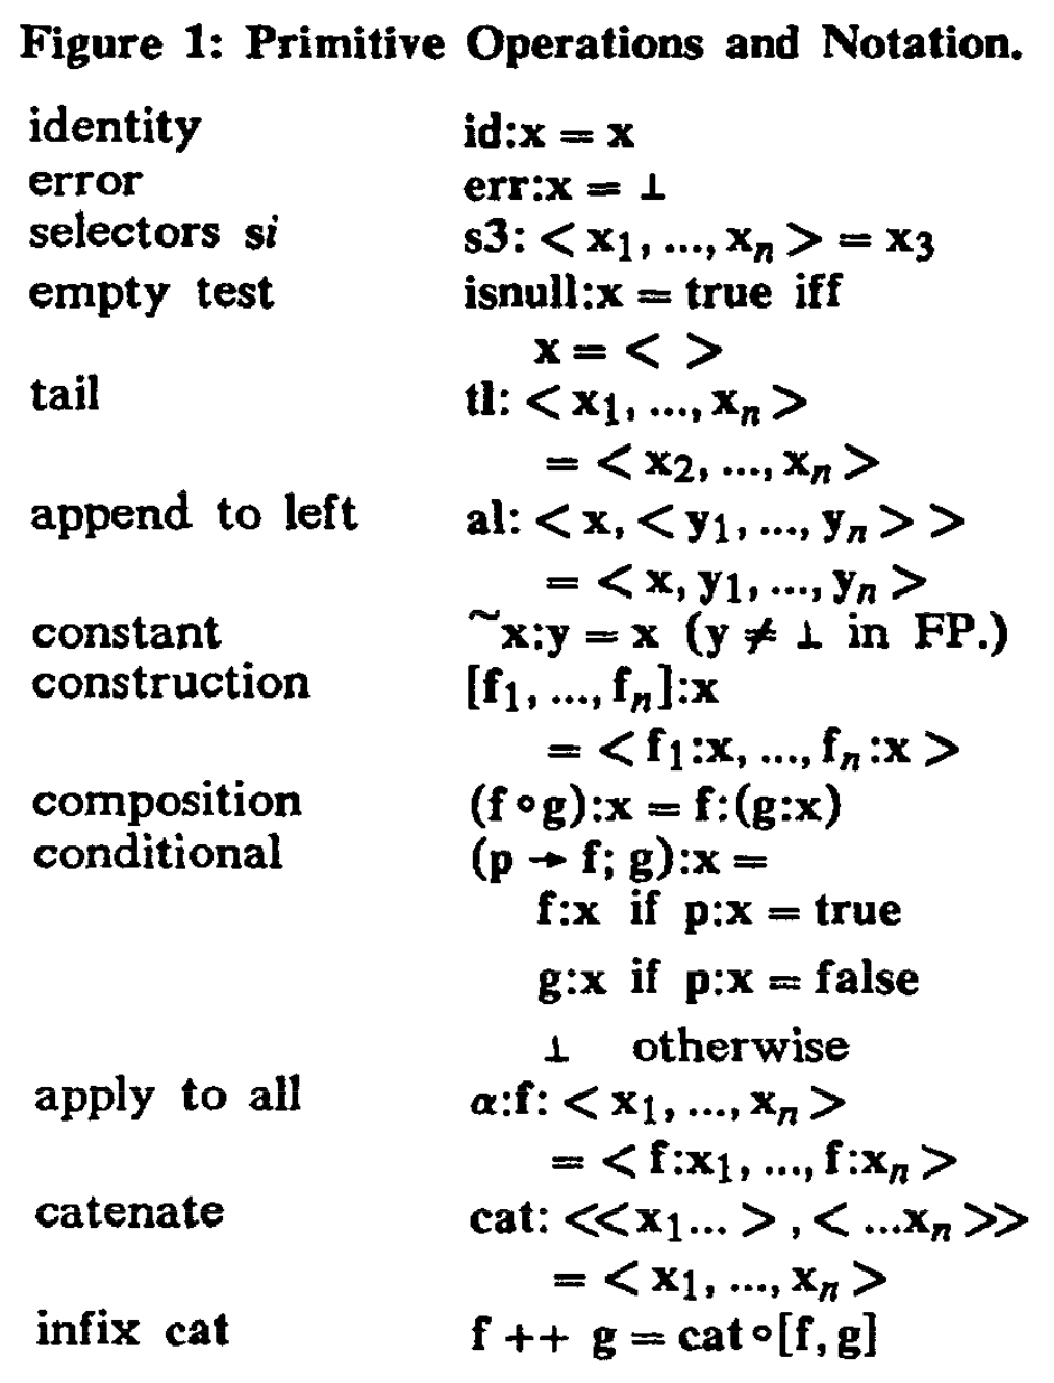
\includegraphics[width=2in]{chapter-01/figs/FP.pdf} \hfill~
\caption{The primitive operations (combining forms) and notations~\cite{10.1145/73560.73575} of FP programs. The semantics of FP is embodied in an underlying algebra of programs, a set of function level equalities that may be used to transform programs and to reason about them.}
\label{fig:1:FP}
\end{figure}


A simple \emph{functional programming} (FP) system is described in~\cite{10.1145/359576.359579}. It is based on combining forms for building programs from simpler programs. An \emph{algebra of programs} is described whose variables denote FP functional programs and whose "operations" are FP functional forms, the combining forms of FP programs, to support the function-level programming paradigm. It allows building programs from a set of generally useful primitives and avoiding named variables. Only programs, aka functions, may be named. In Figure~\ref{fig:1:FP} we display the algebraic rules of FP.

FL (short for ``Function Level’’) is a programming language created by IBM Research at Almaden.
FL is the result of the effort~\cite{BWW90} to design a practical functional programming language based on Backus’ FP.  
FL is intended to be a programming language in which it is easy to write clear, concise,
and efficient programs. FL is designed around a rich set of functionals, forms for combining
existing programs to construct new ones. This emphasis on programming at the function
level results in programs that have a rich mathematical structure useful in reasoning about
and optimizing programs~\cite{IBM:RJ7100}.
A short description of FL combining forms  and primitive functions is given below, where its geometric extension with Julia’s functional syntax is discussed.


\section{FL-based PLaSM in Julia syntax}\label{sect:2-2}

Here we gives a brief informal description of the |Plasm| language~\cite{Paoluzzi:1995:GPP:212332.212349,Paoluzzi2003a}, together with few examples. The section is intended to acquaint the reader with the syntax and style of |Plasm| programs without going into details. 

The interpreter and interactive GUI for PLASM were developed at the Sapienza University of Rome in the 1990s, extending the FL syntax and semantics with the only addition of a geometric type called HPC (hierarchical polyhedral complex) and supporting the FL programming style for geometric computing within the wide domain of Computer-Aided Design.

The book GP4CAD (Geometric programming for CAD)~\cite{Paoluzzi2003a} provides some hundreds of small, simple programs using the FL syntax.

In the past decade, the command-line user interface (CLI), the geometric computational kernel, and the interactive visualizer of ``classic’’ |Plasm| were ported to Python~\cite{pyplasm:2018} and C++, respectively, mainly using the functional features of such languages \cite{dia-report:2009}. Analogously, in recent times, a native and extended port to Julia is being carried out~\cite{plasm:2023}, used in this book, and briefly described in the following, abridged in a few general points.

\begin{enumerate}
\item Function \emph{application} and binary function \emph{composition} are native in Julia, which provides  |f($x$)| and  |g${}\circ{}$f|, respectively.
\item FL \emph{sequence} |<$x_1, x_2, \ldots, x_n$>| is implemented as array |[$x_1, x_2, \ldots, x_n$]|.
\item All primitive functions (programs) are \emph{pure} (without side effects) and written \emph{uppercase}, while named expressions have capitalized names. 
\item Each |Plasm| function is \emph{unary}, possibly using an array of arguments. 
\item The geometric types |Hpc| and |Lar| are extended with an optional Julia’s dictionary of properties.
\end{enumerate}

The point $d.$ is sometime relaxed in Julia |Plasm|, to reduce the visual rumor.
From~\cite{Paoluzzi2003a}, where the interested reader may find many codes discussed in this book in their FL version,  we recall that significant advantages are obtained with this approach in the style and efficiency of program development.
More generally, it is well known that functional programming enjoys several good properties:

\begin{itemize}
\item 
The set of syntax rules of a functional language is very small.
\item 
Each rule is very simple.
\item 
The program code is terse and clear.
\item 
The meaning of a program is well understood, since there is no state. 
\item 
Functions may be used both as programs and as data.
\item 
Programs are easily connected by concatenation and nesting.
\end{itemize}

\subparagraph{Programs are functions}\index{Programs are functions}

Generally speaking, a |Plasm| program is a \textit{function}.  When
\emph{applied} to some input \textit{argument}, a program
produces some output \textit{value}.  Two programs are usually
connected by using functional composition, so that the output of the
first program is used as input to the second program. Starting from here we use the Julia syntax.

\subparagraph{Program composition and application}\index{Program composition and application}

The composition of |Plasm| functions, i.e., |FL| programs with Julia syntax, works exactly as the composition of mathematical functions.  E.g., the application of the
composite mathematical function $f \circ g$ to the $x$ argument
\[
(f \circ g)(x) \equiv f(g(x))
\]
means that the function $g$ is first applied to $x$ and that the 
function $f$ is then applied to the value $g(x)$.  The Julia |Plasm| notation 
for the previous expression is:
\begin{lstlisting}[language=JuliaLocal, style=julia, mathescape = true]
(f${}\circ{}$g)(x) $\equiv$ f(g(x))
\end{lstlisting}
where $\circ$ stands for binary function \textit{composition} and  
|g(x)| stands for \textit{application} of the function |g| to the 
argument |x|. Both notations are Julia’s native.


\subparagraph{Naming objects}\index{Naming objects}

In |Plasm|, a name can be assigned to every value generated by the
language, by using an (unmutable) \emph{definition} construct, either with or without
explicit parameters.  In both cases the so-called \textit{body} of the
definition, i.e.~the expression which follows the definition
\emph{head}, at the right hand of the ``|=|” symbol, will
describe the computational process which generates the  \emph{value}
produced by the computation.  The parameters which it
implicitly/explicitly depends on may be embedded in such a definition.
For example, we may have:
\begin{lstlisting}[language=JuliaLocal, style=julia, mathescape = true]
object = (Fun3 $\circ$ Fun2 $\circ$ Fun1)(params);
\end{lstlisting}
The computational process which produces the |object| value can be 
thought as the computational pipeline shown in 
Figure~\ref{fig:1:5:pipeline}.
\begin{figure}[htbp] %  figure placement: here, top, bottom, or page
   \centering
   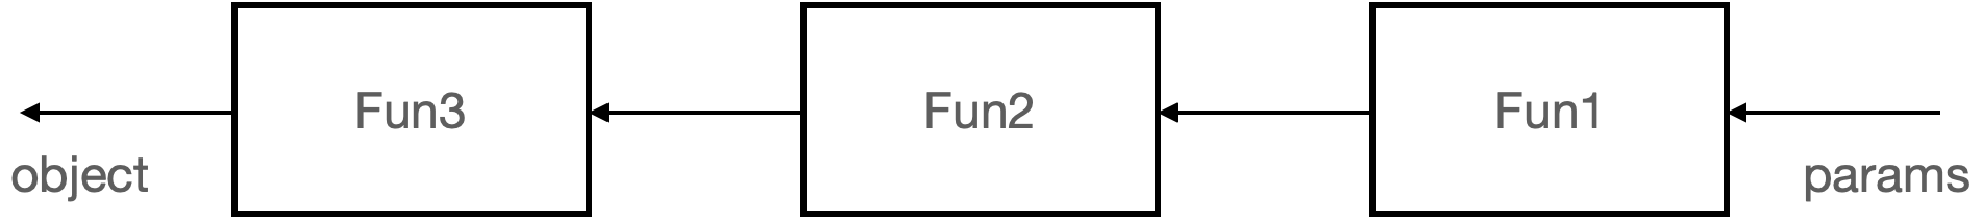
\includegraphics[width=0.8\textwidth]{chapter-01/figs/pipeline.pdf} 
	\caption{Example of computational pipeline}
   \label{fig:1:5:pipeline}
\end{figure}

In this example, the reliance of the model on the 
parameters is implicit.  To modify the generated object value 
it is necessary (a) to change the source code in either the body or 
the local environment of its generating function; (b) to compile the 
new definition; and (c) to evaluate again the object identifier.

\subparagraph{Parametrized objects}\index{Parametrized objects}

A \textit{parametric} geometric model can be defined, and easily
combined with other such models, by using a generating function with
{formal} \emph{parameters}.  Such kind of function may be instanciated
with different {actual} \emph{arguments}, thus obtaining different
output values.  For example, we may have:
\begin{lstlisting}[language=JuliaLocal, style=julia, mathescape = true]
object(params) = (Fun3 $\circ$ Fun2 $\circ$ Fun1)(params);

obj1 = object([p$_{1}$, p$_{2}$, $\ldots$ , p$_{n}$];
obj2 = object([q$_{1}$, q$_{2}$, $\ldots$ , q$_{n}$];
\end{lstlisting}
It is interesting to note that the generating function of a geometric
model may accept parameters of \emph{any} type, including other
geometric objects.



\section{Geometric Programming at Function Level}\label{sect:2-3}

As we already know, |Plasm| is a geometry-oriented extension of a subset of
the |FL| language~\cite{BWW90,IBM:RJ7100}, which is a pure
functional language based on combinatory logic \href{https://en.wikipedia.org/wiki/Combinatory_logic}{[Wikipedia]}.  In particular, the
|FL| language makes use of both pre-defined and user-defined
\emph{combinators}, i.e. higher-order functions which are applied
to functions to produce new functions.  The small but very significant
|FL| subset which is used as the base environment of |Plasm| is summarized
in this section.  

Notice that here and in the remainder of this book the infix symbol
$\equiv$ is normally used to tell the reader that the
\emph{expression} on its left side evaluates to the \emph{value} on
its right side.  Sometimes this symbol is also used to denote an
equivalence between syntactical forms.




\subsubsection*{Elements of {FL} syntax in Julia}\index{Elements!of FL syntax}
\label{sec:FLsyntax}


Primitive |FL| \emph{objects} are characters, numbers and truth values.  Primitive objects added to it by |Plasm| are |Hpc| and |Lar| geometric values, discussed in following chapters.
Primitive objects, functions, applications and sequences are 
\emph{expressions}.
\emph{Sequences} are expressions separated by commas and contained within a pair
of square brackets (Julia |Vector| type):
\begin{lstlisting}[language=JuliaLocal, style=julia, mathescape = true]
[5, fun]
\end{lstlisting}

 An \emph{application} expression |exp1(exp2)| applies the 
\emph{function} resulting from the evaluation of |exp1| on the 
\emph{argument} resulting from the evaluation of |exp2|.  Julia 
allows some binary functions to be used both in infix and prefix form:
\begin{lstlisting}[language=JuliaLocal, style=julia, mathescape = true]
1 + 3 $\equiv$ +(1,3) $\equiv$ 4
\end{lstlisting}

 Application associates to left, i.e.~a sequence of repeated 
applications is evaluated from left to right. Note that this is only 
possible if all the applications, but possibly the last one, generate a 
new function to be applied to the next argument:
\begin{lstlisting}[language=JuliaLocal, style=julia, mathescape = true]
f(g)(h) $\equiv$ (f(g))(h)
\end{lstlisting}

 Application binds stronger than composition, i.e.~applications 
are evaluated first before compositions, as it is shown in the 
following example.  Of course the application of |f| must generate a function value:
\begin{lstlisting}[language=JuliaLocal, style=julia, mathescape = true]
f(g) $\circ$ h $\equiv$ (f(g) $\circ$ h)
\end{lstlisting}


\subsubsection*{Combining forms and functions}\index{Combining forms and functions}
\label{subsec:2:forms}

The function level approach to programming of |FL| emphasizes the
definition of new functions by combining existing functions in various
ways.  The result of this approach is a programming style based on
function-valued expressions.  Some important |FL| \emph{combining
forms} and functions follow.

\subparagraph{Construction}\index{Construction}

The combining form |CONS| allows application of a sequence
of functions to an argument, so producing a sequence of applications:  
\begin{lstlisting}[language=JuliaLocal, style=julia, mathescape = true]
CONS([f$_{1}$,...,f$_{n}$])(x) $\equiv$ [f$_{1}$(x),...,f$_{n}$(x)]
\end{lstlisting}
A |CONS|ed sequence of functions is a sort of \emph{vector function},
that can be composed with other functions and that can be applied to
data.  

E.g., |CONS([sin,cos,tan,atan])| when applied
to the argument |π| returns the sequence of applications
\begin{lstlisting}[language=JuliaLocal, style=julia, mathescape = true]
CONS([sin,cos,tan,atan])(π) 	#=
4-element Vector{Float64}:
  0.0
 -1.0
  0.0
  1.2626272556789115 	=#
\end{lstlisting}

\subparagraph{Apply-to-all}\index{Apply-to-all}
The combining form |AA| has a symmetric effect, i.e. it
applies a function to a sequence of arguments giving a sequence of applications. It is equivalent to the functional |map|  of other languages, Julia included:
\begin{lstlisting}[language=JuliaLocal, style=julia, mathescape = true] 
AA(f)([x$_{1}$,...,x$_{n}$]) $\equiv$ map(f, [x$_{1}$,...,x$_{n}$]) $\equiv$ [f(x$_{1}$),...,f(x$_{n})$]
\end{lstlisting}
For example, we may apply the trigonometric |SIN| function to all the elements of a 
list of numeric expressions:
\begin{lstlisting}[language=JuliaLocal, style=julia, mathescape = true] 
AA(SIN)([0, π/3, π/6, π/2]) 
$\equiv$ [SIN(0), SIN(π/3), SIN(π/6), SIN(π/2)]
$\equiv$ [0, 0.8660254037844382, 0.49999999999999956, 1.0];
\end{lstlisting}
The reader should notice that numeric computations often introduce
round-off and approximation errors.  Just remember that $\pi$ is an
irrational number and cannot be represented exactly by using finite
precision arithmetic.  Also, functions like |SIN| are computed
by using some truncated series expansion.

\subparagraph{Identity}\index{Identity}
The function  returns its argument unchanged
\begin{lstlisting}[language=JuliaLocal, style=julia, mathescape = true] 
ID(x) $\equiv$ x
\end{lstlisting}
In other words, the application of the identity function to \emph{any} argument, 
gives back the same argument:
\begin{lstlisting}[language=JuliaLocal, style=julia, mathescape = true] 
ID(0.5) $\equiv$ 0.5
ID(SIN) $\equiv$ SIN  
ID(SIN)(0) $\equiv$ SIN(0) $\equiv$ 0 
\end{lstlisting}


\subparagraph{Constant}\index{Constant}

The combining form |K| is evaluated as follows, for
whatever |x$_{1}$| and |x$_{2}$|: 
\begin{lstlisting}[language=JuliaLocal, style=julia, mathescape = true]
K(x$_{1}$)(x$_{2}$) $\equiv$ x$_{1}$
\end{lstlisting}
In other words, the first application returns a constant function of
value |x$_{1}$|, i.e.~such that when applied to \emph{any}
argument |x$_{2}$|, \emph{always} returns |x$_{1}$|. 
Some concrete examples follow:
\begin{lstlisting}[language=JuliaLocal, style=julia, mathescape = true] 
K(0.5) $\equiv$ Anonymous-Function 
K(0.5)(10) $\equiv$ 0.5 
K(0.5)(100) $\equiv$ 0.5 
K(0.5)(SIN) $\equiv$ 0.5 
\end{lstlisting}


\subparagraph{Composition}\index{Composition}

The binary composition of functions |COMP|, denoted in Julia by the symbol 
``|∘|”, is defined in the standard mathematical way, as we already know:
\begin{lstlisting}[language=JuliaLocal, style=julia, mathescape = true]
(f $\circ$ g)(x) $\equiv$ f(g(x))
\end{lstlisting}
where |∘| is obtained via the \LaTeX\ expression |\circ| followed by |TAB| character. 
This important typing mechanism is standard in Julia and allows the program code to use Greek letters and many mathematical symbols. 
The \emph{$n$-ary composition} of functions is also allowed:
\begin{lstlisting}[language=JuliaLocal, style=julia, mathescape = true]
COMP([f, g, h])(x) $\equiv$ (f $\circ$ g $\circ$ h)(x) $\equiv$ f(g(h(x)))
\end{lstlisting}
In the following we have, where |π|, |COS| and
|ACOS| are the |Plasm| denotations for Julia’s $\pi$, |cos| and
|acos| \footnote{Which can be directly used in the \texttt{PLASM} code, of course.}, respectively:
\begin{lstlisting}[language=JuliaLocal, style=julia, mathescape = true]
(ACOS $\circ$ COS)(π) $\equiv$ ACOS(COS(π)) $\equiv$ ACOS(-1) $\equiv$ 3.141592653589793
(COS $\circ$ ACOS)(-1) $\equiv$ COS(ACOS(-1)) $\equiv$ COS(3.141592653589793) $\equiv$ -1
COMP([acos, cos, acos])(-1) $\equiv$ ACOS(COS(ACOS(-1))) $\equiv$ 3.141592653589793
\end{lstlisting}



\subparagraph{Conditional combinator}\index{Conditional}

This combinator has the
following semantic: ``|IF| the predicate |p| applied to object 
|x| is |true|, |THEN| apply |f| to
|x|; |ELSE| apply |g| to |x|". 
This construct is very useful when it is necessary to apply different
actions to input data depending on the value of some predicate
evaluated on them, and is possibly more ``natural" than the
conditional statements available in other languages.  

Formally, the conditional form |IF([ p, f, g ])| is evaluated as follows: 
\begin{lstlisting}[language=JuliaLocal, style=julia, mathescape = true]
IF([ p, f, g ])(x) 
	$\equiv$ f(x) if p(x) $\equiv$ TRUE
	$\equiv$ g(x) if p(x) $\equiv$ FALSE
\end{lstlisting}

From a syntax viewpoint, we remark that the |IF| operator is
a higher-order function that \emph{must} be applied to a
\emph{triplet of functions} in order to return a function which is in
turn applied to the input data.

A \emph{predicate} is a
function |p: T $\to \{true,
false\}\ \mbox{where}$ T $\mbox{is a}$ Type|.  Both
|true| and |false| are called \emph{truth values}, and
in Julia are |Bool| values. The predicate |p| is a \emph{function}, as well |f| and |g|,
to be alternatively executed depending on the truth value of the logical
expression |p(x)|.  E.g., we have:
\begin{lstlisting}[language=JuliaLocal, style=julia, mathescape = true]
    IF([ISINTPOS, K(true), K(false)])(1000) $\equiv$ true
    IF([ISINTPOS, K(true), K(false)])(-1000) $\equiv$ false
\end{lstlisting}
where |ISINTPOS| is a predefined predicate that returns |true| 
when applied to some positive integer. 


\subparagraph{Insert Right/Left}\index{Insert Right/Left}
The combining forms |INSR| and |INSL| allow the user to apply
a \emph{binary} function |f|, with signature\footnote{The \emph{signature}
of a function $f$ from a \emph{domain} $A$ to a \emph{codomain} $B$ is
the ordered pair of sets $(A,B)$.  It is normally associated to $f$ by
writing $f : A \rightarrow B$.} |f: D${}\times{}$D $\to$ D|, on a sequence
of arguments of \emph{any} length $n$. In other words, implicitly it is: |INSR(f): D$^n\to$ D|. Note that in the right-hand 
expressions below, |f| is always applied esplicitly  to a \emph{pair} of arguments:
\begin{lstlisting}[language=JuliaLocal, style=julia, mathescape = true] 
INSR(f)([x$_{1}$, x$_{2}$,$\ldots$, x$_{n}$]) $\equiv$ f([x$_{1}$, INSR(f)([x$_{2}$,$\ldots$, x$_{n}$])]) 
INSL(f)([x$_{1}$,$\ldots$, x$_{n-1}$, x$_{n}$]) $\equiv$ f([INSL(f)([x$_{1}$,$\ldots$, x$_{n-1}$]), x$_{n}$])
\end{lstlisting}

An interesting use example of the |INSL| combinator is given
below, where the function |BIGGER| : |Num| $\times$
|Num| $\to$ |Num| is defined.  The
|BIGGER| function returns the maximum of \emph{two} arguments; 
the |BIGGEST: Num|$^n \to$ |Num|  does the same from a list
of arguments of \emph{arbitrary length}:
\begin{lstlisting}[language=JuliaLocal, style=julia, mathescape = true] 
BIGGER   # predefined function
BIGGEST  = INSL(BIGGER)
SMALLER  # predefined function
SMALLEST = INSL(SMALLER)

BIGGER([-10, 0]) $\equiv$ 0 
BIGGEST([-10, 0, -100, 4, 22, -3, 88, 11]) $\equiv$ 88
\end{lstlisting}



\subparagraph{Catenate}\index{Catenate}
The |CAT| function appends to the first one any number of input sequences, so creating
a single output sequence:
\begin{lstlisting}[language=JuliaLocal, style=julia, mathescape = true]
CAT([[10,30,20],[11],[-7,8,12]]) $\equiv$ [10,30,20,11,-7,8,12])
\end{lstlisting}
A pair of concrete examples of how the |CAT| function is used
follows.  The second one is quite interesting: it gives a \emph{filter}
function used to select the non-negative elements of a number
sequence:
\begin{lstlisting}[language=JuliaLocal, style=julia, mathescape = true]
CAT([[10,30,20],[11],[-7,8,12]]) == [10,30,20,11,-7,8,12] 	#=
true	=#
(CAT ∘ AA(IF([ LT(0), K([]), ID ])))([-101,23,-37.02,0.1,84])
$\equiv$ CAT([ [], [23], [], [0.1], [84] ]) 
$\equiv$ [23, 0.1, 84]
\end{lstlisting}
It is useful to \emph{abstract} a |filter| function
with respect to a |predicate| and to an 
argument |sequence|, by showing this function semantics
where curried |LE| stands for \emph{less or equal} to its first argument. |LT|, |GE|, |GT| are similar.

\begin{lstlisting}[language=JuliaLocal, style=julia, mathescape = true]
FILTER(predicate)(sequence)
FILTER(LE(0))([-1,0,1,2,3,4]) == [-1, 0] # => true
\end{lstlisting}

\subparagraph{Distribute Right/Left}\index{Distribute Right/Left}
The functions |DISTR| and |DISTL|  are
defined as:  
\begin{lstlisting}[language=JuliaLocal, style=julia, mathescape = true]
DISTR([[a,b,c], x]) $\equiv$ [[a,x], [b,x], [c,x]]
DISTL([x, [a,b,c]]) $\equiv$ [[x,a], [x,b], [x,c]]
\end{lstlisting}
They accordingly transform a \emph{pair}, constituted by an arbitrary
expression  and by an arbitrary sequence, into a \emph{sequence
of pairs}.
\end{lstlisting}


\begin{script}
Let us give an example of |Plasm| use. The Euler number $e$ is defined as the 
sum of a series of numbers. In particular:
\[
e = {1\over 0!} + {1\over 1!} + {1\over 2!} + \cdots + {1\over n!} + \cdots
\]
We compute an \emph{approximation} of $e$, named |euler|,
as the sum of the first $21$ terms of the series.  The |factorial| function is native in 
Julia:
\begin{lstlisting}[language=JuliaLocal, style=julia, mathescape = true]
    euler = (ADD ∘ AA(DIV) ∘ DISTL)([1, AA(factorial)(0:20)])
\end{lstlisting}
The number 20 is the highest positive integer for which the expression |factorial(20)| does not overflow out of memory assigned to an |Int64| number. In Julia, you can use a type |BigInt| with the |big| function, converting a number to a maximum precision representation. 
Hence, redefine |factorial| as the |FACT| function below, which uses the \emph{ternary conditional} statement:

\begin{lstlisting}[language=JuliaLocal, style=julia, mathescape = true]
FACT(n) = n>0 ? *(1:big(n)...) : 1	#=
Fact (generic function with 1 method)	=#
FACT(100) #=
933262154439441526816992388562667004907159682643816214685929
638952175999932299156089414639761565182862536979208272237582
51185210916864000000000000000000000000	=#
\end{lstlisting}

\begin{coding}[Computation by substitution]
The |euler| value is computed here by successive substitutions. Of course, the
Julia’s optimizing compiler might do a much better job:
\begin{lstlisting}[language=JuliaLocal, style=julia, mathescape = true]
euler = (ADD ∘ AA(DIV) ∘ DISTL)([1,AA(FACT)(0:9)])
$\equiv$ (ADD ∘ AA(DIV) ∘ DISTL)([1, AA(FACT)([0, 1, 2,$\ldots$, 8, 9])])
$\equiv$ (ADD ∘ AA(DIV) ∘ DISTL)([1, [FACT(0),FACT(1),$\ldots$,FACT(9)])])
$\equiv$ (ADD ∘ AA(DIV) ∘ DISTL)([1, [1,1,2,6,$\ldots$,40320,362880]])
$\equiv$ (ADD ∘ AA(DIV)(DISTL([1, [1,1,2,6,$\ldots$,40320,362880]]))
$\equiv$ (ADD ∘ AA(DIV)([[1,1], [1,1], [1,2], [1,6],$\ldots$,[1,362880]])
$\equiv$ ADD([ 1/1, 1/1, 1/2, 1/6, $\ldots$, 1/40320, 1/362880 ])
$\equiv$ 2.7182815255731922
\end{lstlisting}
\end{coding}

Above, we have seen our first substantial example of |Plasm|, aka |FL| computation, as a sequence of expression transformation using the rules of combinators. The round brackets induce the order of transformations included into an expression and often corresponds to applications. The sub-expressions nested
more deeply are transformed first. When using |Float64|, i.e., 8 bytes, the numeric precision is 15-16 digits.

\vspace{5mm}
A simpler and more elegant implementation of the Euler number is given below, 
where |C| is the currying combinator\footnote{
In mathematics and computer science, \emph{currying} is the technique of translating the evaluation of a function that takes multiple arguments into evaluating a sequence of functions, each with a single argument.}:
\begin{lstlisting}[language=JuliaLocal, style=julia, mathescape = true]
    EULER(n) = (ADD ∘ AA(C(DIV)(1) ∘ FACT))(0:n)
\end{lstlisting}

The best Julia approximation of the Euler number is with |n = 57| terms of the defining series, since all  digits (80) of a |BigFloat| value are exact:

\begin{lstlisting}[language=JuliaLocal, style=julia, mathescape = true]
EULER(56)	#=
2.718281828459045235360287471352662497754969541622429154734
483565013216246202514	=#
EULER(57)	#=
2.718281828459045235360287471352662497754969541622429154734
483565013216246202549	=#
EULER(58)	#= The 58th element of the Euler series
2.718281828459045235360287471352662497754969541622429154734
483565013216246202549	=#
\end{lstlisting}



\section{Julia’s package Plasm.jl}\label{sect:2-4}



After several years of research about Linear Algebraic Representation (LAR) and algebraic operations~\cite{ieee-tase,DBLP:journals/cad/DiCarloPS14,TSAS:2020,PAOLUZZI2023103436} with sparse matrices and solid models, a new Julia package for geometric programming, named Plasm.jl, was developed while writing this book. We aim to finish the software version 1.0 before the book is published. 

The work has mainly consisted of porting to Julia the  Pyplasm library~\cite{pyplasm:2018} written in Python years ago. Of course, both are open-source and downloadable from the web\footnote{Citation of pyplasm and plasm.jl URLs.}. Our software plan is to realize in version 1.0 a significant extension of the language related to computation of space arrangements~\cite{TSAS:2020} and Boolean solid algebras~\cite{PAOLUZZI2023103436}.

Of course, the reader is warmly invited to install the latest version of Julia and to download our package |Plasm.jl| on computational environment. The installation is not strictly necessary since web access will be available. Still, it is always helpful, while learning a new language, to have your own environment where you are free to do any experiment.

\subparagraph{Plasm.jl}
The main file of the package is named as usual with the name |Plasm.jl| of the package itself. Its primary function is to create the run-time executable of |Plasm.jl|, by calling the external references (i.e., the exported functionality) taken from other packages and to include the Julia code of other package files, in our case |fenvs.jl|, |hpc.jl|, and |viever.jl|. Note that its name starts uppercase, according to the Julia’s convention for packages.

\subparagraph{fenvs.jl}
The |fenvs.jl| file, whose name stands for “|f|unctional |env|ironment|s|” implements in Julia the majority of the small exciting programs developed for the GP4CAD book and includes many primitives for surface design with various methods. Other needed functions and functions of general use can be created directly by the reader if savant in computer graphics or CAD.

\subparagraph{hpc.jl}
The primary data structure is the |Hpc| (Hierarchical Polyhedral Complex)~\cite{}, based on convex cells, and extended to allocate general polyhedral cells, i.e., polyhedra of any (low) dimension, connected but generally nonconvex and with interior holes. 
The |hpc.jl| file contains the developed design and implementation of the very general and \emp{multidimensional}  geometric data structure called |Hpc|~\cite{}, that allows to accommodate all the geometric and solid algorithms and tools developed in this book. As we show in the book, the |Hpc| structure is straightforward, versatile, and general. It does not use any of the large number of highly specialized and very complex data structures invented for solid modeling. We will show that our topological approach to geometric computations only needs the linear algebra of sparse matrices and vectors.

\subparagraph{viever.jl}
Finally, the |viewer.jl| file is used as the home of an interactive geometry viewer, used to interact with the shapes generated by Plasm codes either on the terminal screen of a laptop or on the HTML interface of a web browser program. This web viewer version was developed to view the Plasm models on the web and to write rich text examples and exercises within the pages of a web notebook, and hence without the need to install any software.





\section{Julia REPL (Read-Eval-Print-Loop)}\label{sect:2-5}

An interactive language shell is an interactive computer programming environment in a single terminal  that takes user inputs from keyboard or file, executes them, and prints the result to the display. A program developed in REPL terminal environment (CLI -- command language interface) is written and executed piecewise. This approach requires that the language executable code may work as an interpreter, i.e. combining translation of source lines in machine code with immediate execution.
 

\subsubsection*{REPL editor}\label{sect:2-5-1}

Julia comes with a full-featured interactive command-line REPL (read-eval-print loop) built into the julia executable~\cite{}. Once installed, to enter Julia, open a terminal and digit "julia" after the system prompt “\$”. The  acknowledgement in Figure \ref{fig:2:ackplasm}
will appear on the screen. Once the REPL starts, you will be at the Julia prompt. The Julia REPL can operate in different prompt modes:
\begin{itemize}
\item 
Julia mode (the default),
\item 
help mode,
\item 
Pkg mode, and
\item 
shell mode.
\end{itemize}
To enter help, Pkg, or shell mode, place the cursor at the beginning of the Julia mode prompt and type a question mark (?), a closing bracket (]), or a semicolon (;), respectively. 

The help mode is used to get information about the meaning or use (arguments, examples, etc.) of a function, as written by the developer in the function  “docstring”. The Pkg (package) mode covers many things, including managing package installations, developing packages, working with package registries and more. The shell mode allows the terminal user to run shell commands from the Julia |REPL|.

To return to Julia mode, place the cursor at the beginning of the prompt and press Backspace~\cite{repl:Whitaker:2024}.
A simple and very useful interactive blog to start use |REPL| is \href{https://blog.glcs.io/julia-repl#heading-starting-the-julia-repl}{https://blog.glcs.io/julia-repl#heading-starting-the-julia-repl}. 


\begin{figure}
\centering
   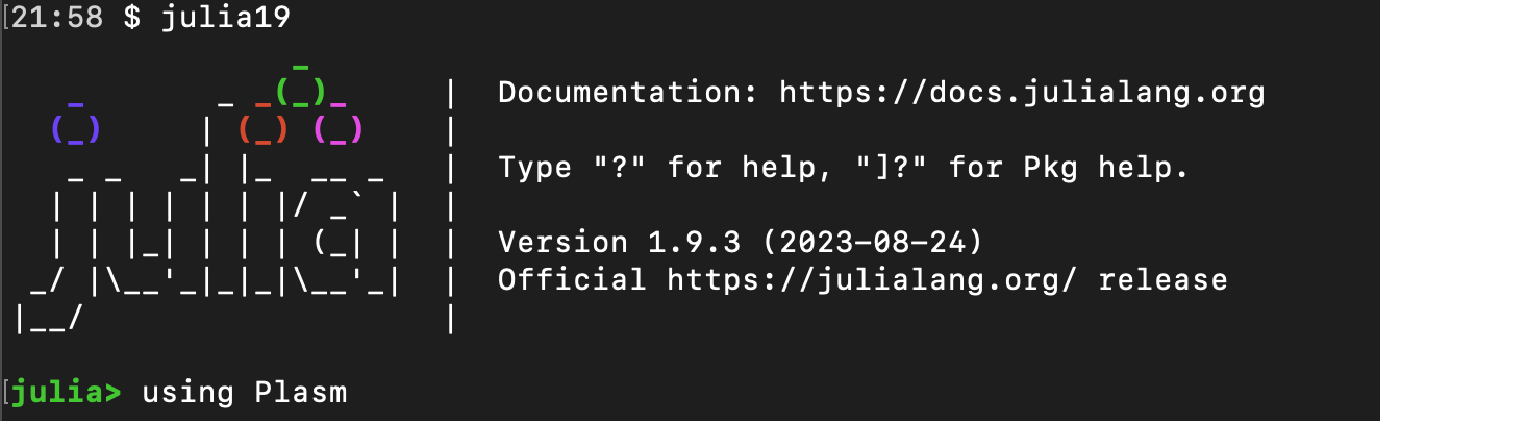
\includegraphics[width=\textwidth]{chapter-02/figs/screen.pdf}%

\caption{To run Julia by invoking its name on the commend-line of the terminal on computer screen. Note the “using Plasm” after the REPL prompt “> julia”.}
\label{fig:2:ackplasm}
\end{figure}





\subsubsection*{OhMyREPL package}\label{sect:2-5-2}

The Julia package \href{https://kristofferc.github.io/OhMyREPL.jl/latest/}{\tt OhMyREPL} hooks into the Julia |REPL| and gives it many new features~\cite{OhMyREPL:jl}. It allows for several enhancements, including:
syntax highlighting; bracket highlighting; bracket completion; rainbow brackets;
markdown syntax highlighting; fuzzy |REPL| history search.



\subsubsection*{Julia REPL workflow}\label{sect:2-5-3}

The most basic Julia workflows involve using a text editor in conjunction with the julia command line. A common pattern includes the following elements:
\begin{enumerate}
 \item 
   Put code under development in a temporary module. Create a file, say |Tmp.jl|, and |include| within it

\begin{lstlisting}[language=JuliaLocal, style=julia, mathescape = true]
    module Tmp
    <your definitions here>
    end
\end{lstlisting}

\item 
    Put your test code in another file. Create another file, say |tst.jl|, which begins with

\begin{lstlisting}[language=JuliaLocal, style=julia, mathescape = true]
    import Tmp
\end{lstlisting}

    and includes tests for the contents of |Tmp|. The value of using |import| versus |using| is that you can call reload("Tmp") instead of having to restart the REPL when your definitions change. Of course, the cost is the need to prepend |Tmp.| to uses of names defined in your module. (You can lower that cost by keeping your module name short.)
    Alternatively, you can wrap the contents of your test file in a module, as

\begin{lstlisting}[language=JuliaLocal, style=julia, mathescape = true]
    module Tst
        using Tmp
        <scratch work>
    end
\end{lstlisting}

\item 
    The advantage is that you can now do |using Tmp| in your test code and can therefore avoid prepending Tmp. everywhere. The disadvantage is that code can no longer be selectively copied to the REPL without some tweaking.

    Lather. Rinse. Repeat. Explore ideas at the julia command prompt. Save good ideas in |tst.jl|. Occasionally restart the |REPL|, issuing

\begin{lstlisting}[language=JuliaLocal, style=julia, mathescape = true]
    include(“Tmp.jl")
    include("tst.jl")
\end{lstlisting}
\end{enumerate}


Julia's REPL provides rich functionality that facilitates an efficient interactive workflow~\cite{}. 


    
    

\section{Geometric Programming examples}\label{sect:2-6}

Here we show a couple of simple examples to show the compactness and expressive power of our geometric language.

\begin{coding}[2D virtual Manhattan] 
\label{example:1:Manhattan2D}

\begin{figure}
\centering
   
\includegraphics[width=0.59\textwidth]{chapter-01/figs/manhattan2d.pdf}%
   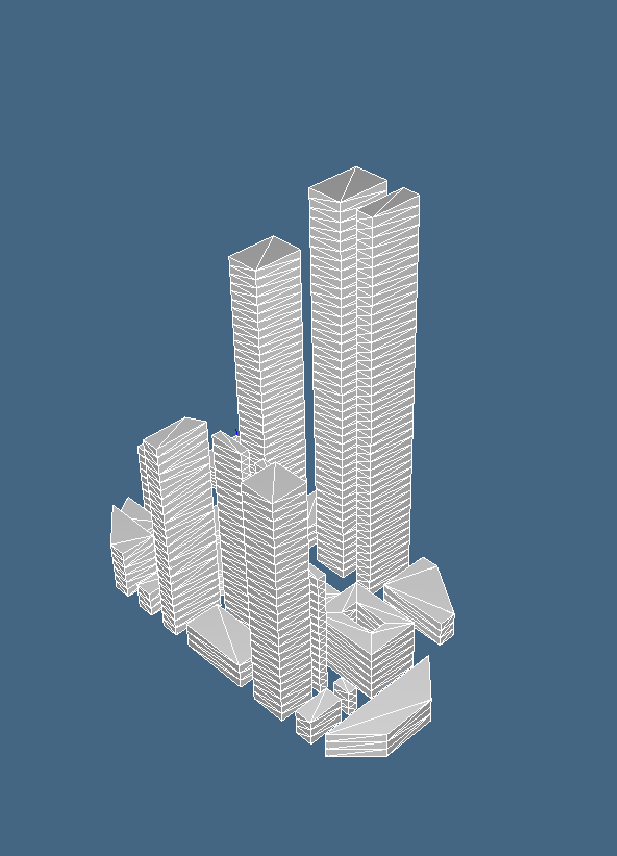
\includegraphics[width=0.41\textwidth]{chapter-01/figs/manhattan3d-1.pdf}

\caption{(a) Hierarchical polyhedral complex (Lar) 2D value embedded in 3D. A perspective projection generates the image. Each connected shape is a polyhedral cell, even nonconvex and with inner holes. Each triangle is a convex cell; (b) 3D Plasm view of the model value of \texttt{Hpc} type discussed in Example~\ref{example:1:Manhattan3D}}
\label{fig:1:FP}
\end{figure}

Of course, we start our geometric modeling session by telling the Julia compiler\footnote{To load \texttt{Plasm} in Julia, open a terminal, start your \texttt{julia} application, and after the prompt \texttt{julia>} write \texttt{using Pkg; Pkg.add("Plasm ")}} to use the |Plasm| package. Then, we give the compiler the code and data that follows, possibly contained in a file |Manhattan2D.jl|.

\begin{lstlisting}[language=JuliaLocal, style=julia, mathescape = true] 
julia> using Plasm
\end{lstlisting} 

We start by defining the 2D coordinates of the vertices of our model. 
\begin{lstlisting}[language=JuliaLocal, style=julia, mathescape = true] 
julia> verts = [[0.,0],[3,0],[5,0],[7,0],[8,0],[9.5,1],[10,1.5],[0,3],
[3,3],[5,3],[7,3],[8,3],[9.5,3],[0,4],[3,4],[5,4],[9.5,4],
[12,4],[9.5,5],[10,5],[12,5],[0,6],[3,6],[5,6],[0,7],[3,7],
[5,7],[9.5,7],[12,7],[9.5,8],[12,8],[0,9],[3,9],[5,9],[8,
9],[9,9],[12,9],[0,10],[3,10],[5,10],[8,10],[9,10],[9.5,10],
[10,10],[12,10],[6,11],[7,11],[0,12],[3,12],[9,12],[9.5,12],
[0,13],[3,13],[6,13],[7,13],[9,13],[9.5,13],[0,14],[3,14],[5,
14],[8,14],[9,14],[9.5,14],[10,14],[12,14],[0,15],[3,15],[5,
15],[8,15],[0,16],[6,16],[7,16],[9,17],[9.5,17],[10,17],[12,
17],[6,18],[7,18],[9,18],[9.5,18],[10,18],[12,18],[2,19],[3,
19],[5,19],[8,19],[9,19],[9.5,19],[10,19],[12,19],[5,20],[12,
20],[7,22],[10,22],[9,6],[12,6],[9,15],[9.5,15],[10,15],[12,
15]]
\end{lstlisting}
Then we give the following description of convex cells of type |Cells = Vector{Vector{Int64}}|:
\begin{lstlisting}[language=JuliaLocal, style=julia, mathescape = true] 
julia> cells = [[1,2,9,8],[3,4,11,10],[5,6,13,12],[14,15,23,22],[16,
17,19,24],[7,18,21,20],[25,26,33,32],[27,95,28,35,34],[95,
96,29,28],[30,31,37,36],[38,39,49,48],[40,41,47,46],[41,61,
55,47],[55,61,60,54],[54,60,40,46],[42,43,51,50],[44,45,65,
64],[52,53,59,58],[56,57,63,62],[66,67,84,83,70],[68,69,72,
71],[69,86,78,72],[78,86,85,77],[71,77,85,68],[97,98,74,
73],[99,100,76,75],[79,80,88,87],[81,82,90,89],[91,92,94,93]]
\end{lstlisting}
Finally, |verts|  and |cells| are transformed in a geometric object of type |Hpc| 
by the function |MKPOL| and stored in the Julia variable named |model|.

\begin{lstlisting}[language=JuliaLocal, style=julia, mathescape = true] 
julia> model = MKPOL(verts,cells)
# Hpc ... ...
\end{lstlisting}
A |model| image is generated by the |Plasm| viewer, within a system window named "Manhattan2D”, for interaction with mouse and arrow buttons. 
\begin{lstlisting}[language=JuliaLocal, style=julia, mathescape = true] 
julia> VIEW( model, "Manhattan2D” )
\end{lstlisting}
From terminal we might write: \$| julia path/Manhattan2D.jl|
\end{coding}



\begin{figure}
   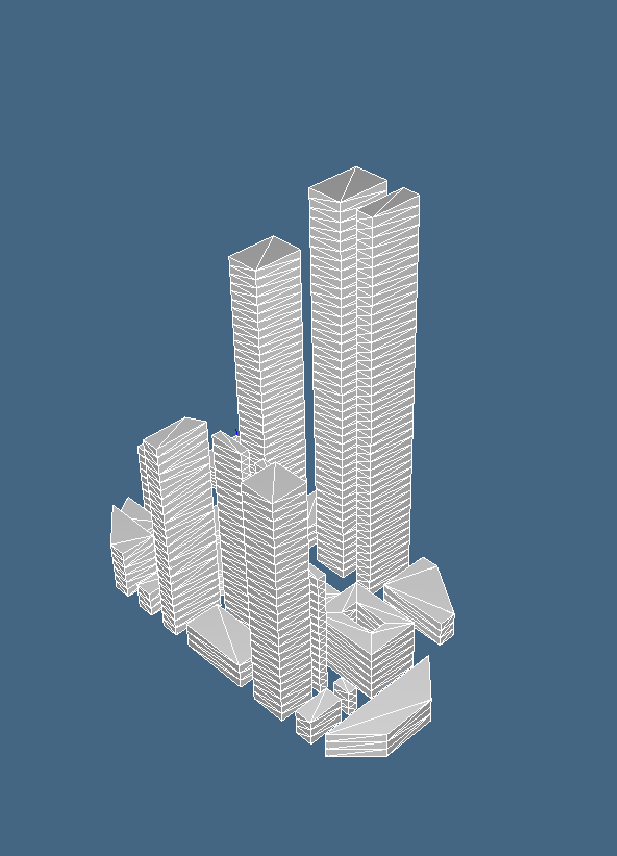
\includegraphics[width=1.955in]{chapter-01/figs/manhattan3d-1.pdf}
   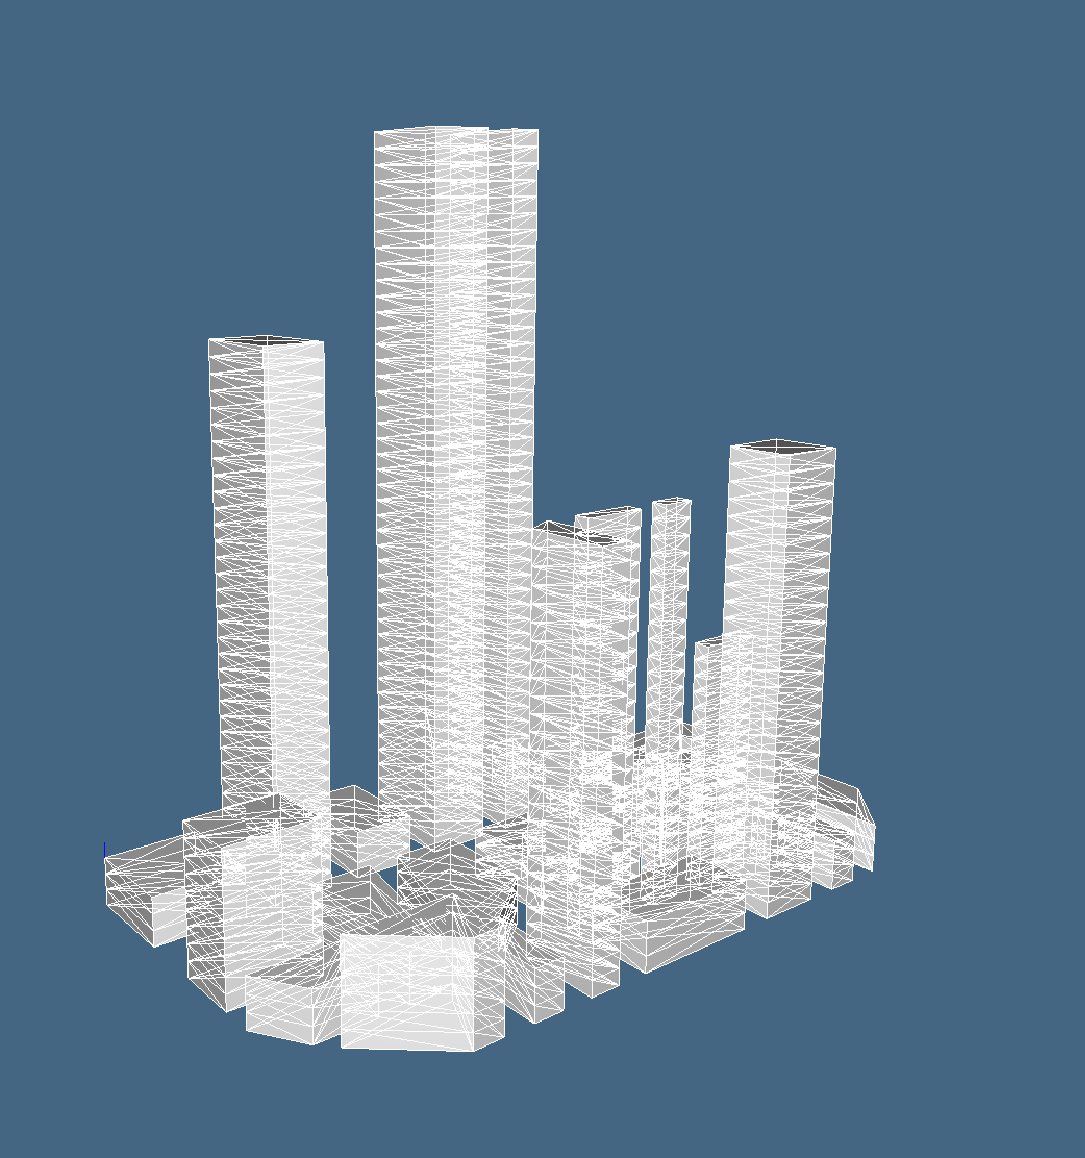
\includegraphics[width=2.55in]{chapter-01/figs/manhattan3d-2.pdf}
\caption{3D model generated by using the 2D \texttt{cells} defined in \texttt{Manhattan2D} example.
 (a) opaque visualization; (b) transparent visualization from a different viewpoint.}
\label{fig:1:FP3D}
\end{figure}

\begin{coding}[3D virtual Manhattan] 
\label{example:1:Manhattan3D}

The model of Figure~\ref{fig:1:FP3D} is given by (1) a vector |ManhattanH| of floor numbers; (2) generation of corresponding 1D and 2D vectors of |Hpc| objects stored in |pols1D| and |pols2D|; (3)~by Cartesian product of corresponding |Hpc| pairs |(2D,1D)|. See below:

\begin{lstlisting}[language=JuliaLocal, style=julia, mathescape = true] 
ManhattanH = [1,3,1,11,1,2,1,1,1,8,15,1,1,1,1,8,1,15,8, 1,2,2,2,2,5,9,1,1,1].*3
# 29-element Vector{Int64}:
storeys = CONS(AA(DIESIS)(ManhattanH))(.5)
# 29-element Vector{Vector{Float64}}:
pols1D = AA(QUOTE)(storeys)
# 29-element Vector{Hpc}:
pols2D = [MKPOL(verts,[cell]) for cell in cells]
# 29-element Vector{Hpc}:
\end{lstlisting}
\begin{lstlisting}[language=JuliaLocal, style=julia, mathescape = true] 
pols3D = AA(splat(*))(TRANS([pols2D, pols1D]))
# 29-element Vector{Hpc}:
VIEW(STRUCT(pols3D), "Manhattan3D")
\end{lstlisting}


In particular, we define an array of virtual heights for each \emph{polygon} of |Manhattan2D|. Such numbers are transformed in repeated |storeys| heights by 
|AA(DIESIS)| (where |DIESIS| was the \texttt{\#} operator in |FL|-based |Plasm|, but it is not usable in Julia, since it denotes comments) and then codified as 1D |Hpc| polyhedra stored in |pols1D| by the |QUOTE| operator. Analogously, a set of 2D polyhedra is stored in the |pols2D| array. The Cartesian product |*| of corresponding |Hpc| objects is stored in |pols3D| array using the Julia’s |splat| function. Finally, a single |Hpc| object is visualized in a system window named |Manhattan3D|. 

It is worth noting that every |polygon*segment| multiplication of two |Hpc| objects produces a new |Hpc| polyhedron of dimension equal to the sum of dimensions of operands.
The reader should not forget that the |Plasm| language and the |Hpc| data structure are both  \emph{multidimensional}.
\end{coding}

We also note that a large number of significant programming examples with Julia and |Plasm| in Julia can be found inside the file |Plasm/fenvs.jl|, and executed in the terminal by writing \$ |julia ./test/fenvs.jl|, being located into the |Plasm.jl directory|, and after having downloaded and installed the package |Plasm.jl| in a recent |julia| environment.



\begin{coding}[Solid 2D graph of a scalar function]
A simple unusual geometric example is given here, showing some of canonical constructs of geometric design with |Plasm|. First, we build and show in Figure~\ref{fig:2:sinmapping}a the  |Domain2D| of the parametric 2D solid |model| given in Figure~\ref{fig:2:sinmapping}b.  The |MAP| operator is applied first to the function |Mapping2D| to be applied to all \emph{vertices} of a cell decomposition of |Domain2D|, in turn generated as the Cartesian product |POWER| of two 1D cellular complexes, so producing a 2D cell complex of the mapped interval |Domain2D| with $36\times 6$ squared cells.


\begin{figure}[htbp]
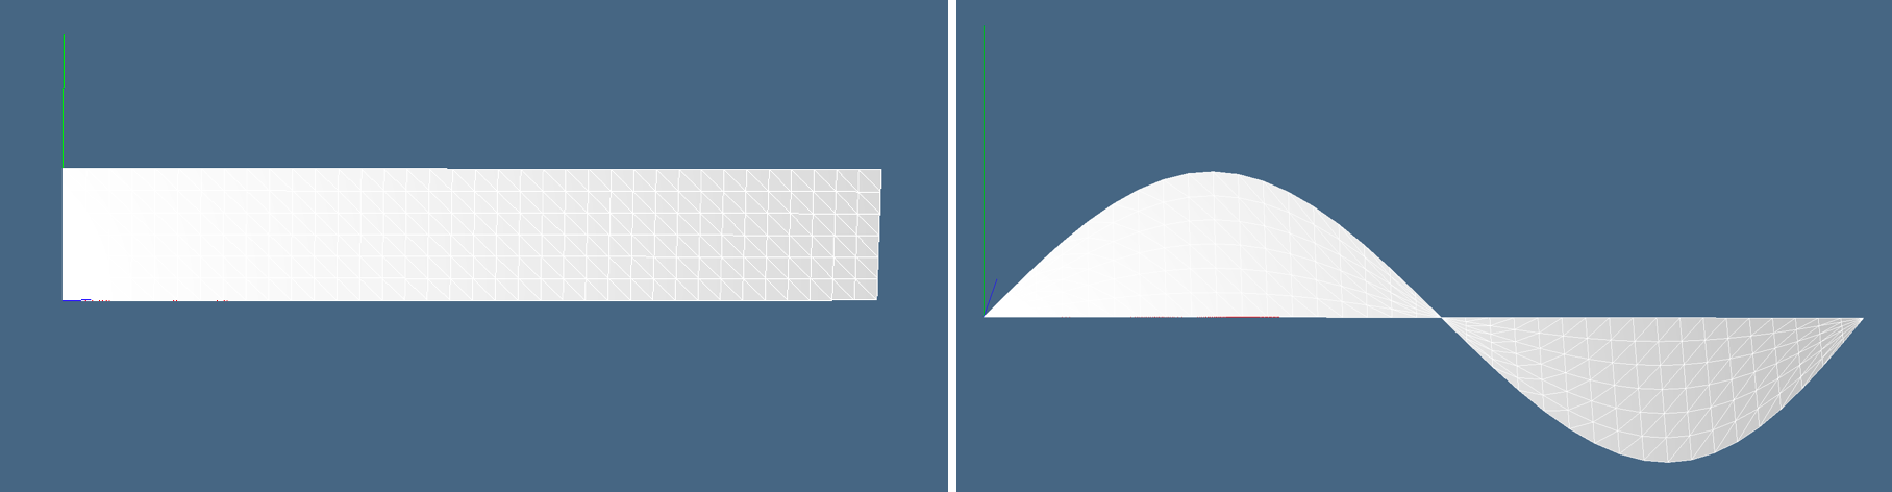
\includegraphics[width=\textwidth]{chapter-01/figs/functionmap} 
\caption{The mapping of a function of two arguments on its 2D parameter domain. Each element (point and cell) of the cellular domain is paired with a corresponding element in the function range. The figure shows how the elements are paired. (a) The cellular complex decomposing the function domain $[2\pi,1]$; (b) the function range transformed after the function \texttt{p->[u,sin(u)*v]} was mapped on the vertices of the 2D domain. }
\label{fig:2:sinmapping}
\end{figure}


\begin{lstlisting}[language=JuliaLocal, style=julia, mathescape = true] 
Domain2D = Power(INTERVALS(2π)(36), INTERVALS(1)(6));
Mapping2D = p->((u,v)=p; [u,sin(u)*v]);
model = MAP(Mapping2D)(Domain2D)
\end{lstlisting}

The two parameters |u,v| of the model domain are worked out by |p->(...)|, anonymous |Julia| function, and applied to each vertex of |Domain2D| by the |MAP| operator.
Two geometric objects Domain2D and model are finally shown and displayed in Figure~\ref{fig:2:sinmapping}:

\begin{lstlisting}[language=JuliaLocal, style=julia, mathescape = true] 
VIEW(Domain2D)
VIEW(model)
\end{lstlisting}


The virtual models of both |Domain2D| and |model|, finally visualized in Figure~\ref{fig:2:sinmapping}, are made available for display by the |Plasm| operator |VIEW|, and can be interactively handled by the user.


%\begin{figure}[tbp]
%\centering
%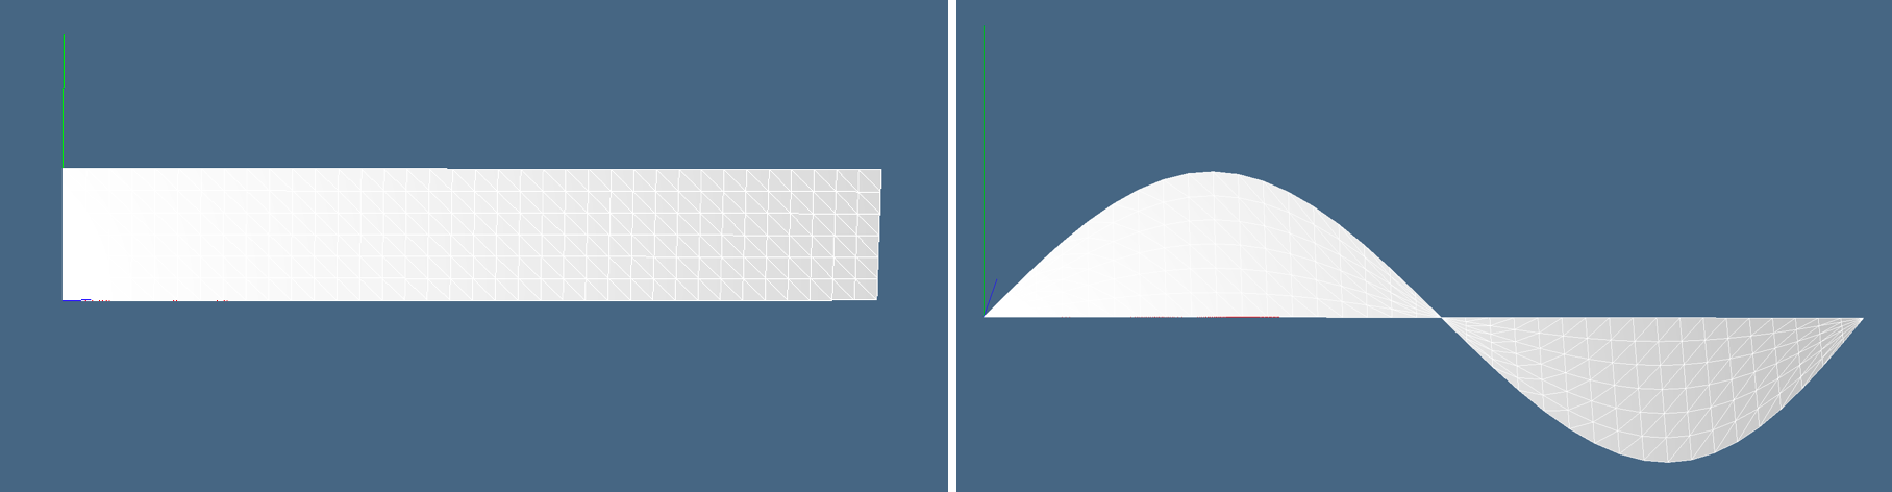
\includegraphics[width=\textwidth]{chapter-01/figs/functionmap.pdf} 
%\caption{The mapping of a function of two arguments on its 2D parameter domain. Each element (point and cell) of the cellular domain is paired with a corresponding element in the function range. The figure shows how the elements are paired. (a) The cellular complex decomposing the domain $[0,2\pi]\times [0,1]$; (b) the range of function \texttt{p->[u,sin(u)∗v]} on the vertices of 2D cellular domain to be mapped by (u,v) $\mapsto$ (x,y). }
%\label{fig:2:sinmapping}
%\end{figure}
\end{coding}


\bibliographystyle{spmpsci}
\bibliography{plasmbook.bib}




% !TEX TS-program = xelatex

\chapter{Geometry and topology primer}
\label{chapt:3}

It is implausible to set up a computer language and computational environment to define and deliver the geometric shape of construction elements and spaces without a pretty good understanding of basic geometric and topological concepts. Hence, this chapter introduces some basic notions about geometric spaces, operators, and properties, like linearity, that provide the computational foundation of shape definition and model construction.
The essential elements of geometric spaces and cellular models, like affine transformations and simplicial, cubical, and polyhedral complexes, constitute the substrate of |Plasm| discourse for building hierarchical assemblies of AEC products of any scale and complexity.

%1234567890234567890234567890234567890234567890234567890234567890234567890
\section{Geometric Spaces}\label{}


In mathematics and science, a space is a set of objects with some added structure.
In this section we discuss the geometrical spaces used to represent inside a computer memory the actual objects of natural, artificial or virtual environments, or better their geometric models, in order to study, visualize and/or simulate some associated physical behavior. 
In particular, we deal in this section with linear, affine, and convex spaces as sets of vectors and/or points with selected properties.

\subsection{Vector space}
\label{subsec:2:style}

The concept of vector space is undoubtedly the most helpful instrument of mind invented by mathematicians for scientists, engineers, and architects, to represent and study formally or graphically both the primary and complex arrangements and behaviors of our natural and artificial environment.

\subsubsection*{Definition}

A \emph{vector space} (or \emph{linear space}) $\mathcal{V}$ over a field $\mathcal{F}$ is a set, closed w.r.t. two composition rules (the output of composition belongs to the set of inputs).

%$+ : \mathcal{V} \times \mathcal{V} \to \mathcal{V}$ \hfill (addition: internal composition)
%
%$\cdot : \mathcal{F} \times \mathcal{V} \to \mathcal{V}$ \hfill (product by a scalar: external composition)
%
%such that, for each $\v{u}, \v{v}, \v{w} \in \mathcal{V}$ and for each scalar $\alpha, \beta \in \mathcal{F}$, the rules $+, \cdot$ satisfy the following
%axioms:
%\begin{quote}
%\begin{enumerate}
%\item  $\v{v} + \v{w} = \v{w} + \v{v}$; \hfill (commutativity of addition)
%\item  $\v{u} + (\v{v} + \v{w})=(\v{u} + \v{v}) + \v{w}$;  \hfill (associativity of addition)
%\item  there is a $\v{0} \in \mathcal{V}$ such that $\v{v} + \v{0} = \v{v}$; \hfill (neutral element of addition)
%\item  there is a $-\v{v} \in \mathcal{V}$ such that $\v{v} + (-\v{v}) = \v{0}$; \hfill (inverse of addition)
%\item $\alpha \cdot (\v{v} + \v{w}) = \alpha \cdot \v{v} + \alpha \cdot \v{w}$; \hfill (distrib. of addition w.r.t. product)
%\item $(\alpha + \beta) \cdot \v{v} = \alpha \cdot \v{v} + \beta \cdot \v{v}$; \hfill (distrib. of product w.r.t. addition)
%\item $\alpha \cdot (\beta \cdot \v{v})=(\alpha \beta) \cdot \v{v}$; \hfill (associativity of product)
%\item $1 \cdot \v{v} = \v{v}$. \hfill (neutral element of product)
%\end{enumerate}
%\end{quote}
%
%The dot operator to multiply a vector by a scalar will be dropped in the remainder of
%this book, so that the operation will be denoted by the juxtaposition of the arguments.
%Hence we write $\alpha(\beta\, \v{v})$ instead of $\alpha \cdot (\beta \cdot \v{v})$.\\

The elements $\v{v}\in \mathcal{V}$ are called \emph{vectors}, and are often represented by an oriented arrow with given direction, orientation, and length. The elements $\alpha\in\mathcal{F}$ are called \emph{scalars}. The sum of two non-zero vectors $\v{u},\v{v}\in\mathcal{V}$ is a third vector $\v{w} = \v{u}+\v{v}\in\mathcal{V}$ with direction and length different from both $\v{u}$ and $\v{v}$.  We may write $\v{v}+\v{v} = 2\v{v}$, and see here both the operations of a vector space: (a) addition of vectors, and (b) multiplication times a scalar. 

The product of a vector by a scalar $\alpha\, \v{v} = \v{v}\, \alpha \in \mathcal{V}$ is a vector collinear with $\v{v}$ and with different length if $\alpha \not= 1$. This explain the name “scalar” since a number “scales” (change the length of) the vector it multiplies. 

The length of $\v{u} = \alpha\,\v{v}$  grows or shrinks w.r.t. $\v{v}$ according to a positive $0 < \alpha < 1$. If $\alpha < 0$, then $\v{u}$ has orientation opposite to $\v{v}$.

%\begin{lstlisting}[language=JuliaLocal, style=julia]
%using Distributions
%
%function thompson_sampling(𝛂, 𝛃, apply; T=100)
%    for t in 1:T
%        𝛉 = rand.(Beta.(𝛂, 𝛃))
%        x = argmax(𝛉)
%        r = apply(x)
%        𝛂[x], 𝛃[x] = (𝛂[x] + r, 𝛃[x] + 1 - r)
%    end
%    return Beta.(𝛂, 𝛃)
%end
%\end{lstlisting}


\subsubsection*{Linear independence}

A \emph{linear combination} of vectors is a new vector that is defined as a sum of scalar multiples of other vectors.
Let $\v{v}_1, \v{v}_2,..., \v{v}_n \in \mathcal{V}$ and $\alpha_1, \alpha_2,...,\alpha_n \in \mathcal{F}$, with $\mathcal{V}$ a vector
space on the field $\mathcal{F}$ of scalar numbers. The vector 
\[
\v{w} = \alpha_1 \v{v}_1 + \alpha_2 \v{v}_2 + \cdots + \alpha_n \v{v}_n = \sum^n_{i=1}
	\alpha_i \v{v}_i \in \mathcal{V}
\]
is called a linear combination of vectors $\v{v}_1, \v{v}_2,..., \v{v}_n$.

\begin{itemize}
\item Two or more vectors are said \emph{linearly independent} if none of them can be written as a linear combination of the others;
\item if at least one of them can be written as a linear combination of the others, then they are said \emph{linearly dependent}.
\end{itemize}

Given a set of vectors, you can determine if they are linearly independent by writing the vectors as the columns of a matrix $\T{A}$, and solving $\T{A}\,\v{x} = \v{0}$. 

If there are non-zero solutions, then the vectors are linearly dependent. If the only solution is $\v{x} = \v{0}$, then they are linearly independent.

The typical vector spaces in this book will be (a) the numeric field $\mathbb{R}$ for scalars and $\mathbb{R}^n$ for vector coordinates, with (b) $\dim = d$, for $0\leq d\leq 3$.

\subsubsection*{Examples}


\begin{coding}[Matrices $m\times n$ are vector spaces].
Generate a random $100\times 100$ matrix |A = rand(100,100)|. The default of |rand()| function are values of type |Float64| in |[0.0,1.0]|, so we ask the compiler to compute the matrix multiplication by the scalar $\pi$, denoted by the Greek symbol. The generated value is shown commented and simplyfied for printing in small space: 

\begin{lstlisting}[language=JuliaLocal, style=julia]
A = rand(100,100) * π 	#=
100x100 Matrix{Float64}:
 0.901069  …  0.172854
 0.357548     0.8537
 ⋮         ⋱  
 0.519136     0.857736 		=#
\end{lstlisting}
\end{coding}

\begin{coding}[Random vector generation.]
Then, we generate a 100-vector of random integers within the interval 
|[0,100]|, by using the Julia |0:100| iterator:

\begin{lstlisting}[language=JuliaLocal, style=julia]
b = rand(0:100, 100) 	#=
100-element Vector{Int64}:
 61
 85
  ⋮
 51			=#
\end{lstlisting}
\end{coding}

\begin{coding}[Multiplication matrix-vector.] This operation is implemented natively and very efficiently for big matrices in Julia, as well the product and the sum of dense matrices (the detail of printing  depends on available space on output screen):
\begin{lstlisting}[language=JuliaLocal, style=julia]
A * b	 	#=
100-element Vector{Any}:
 2786.383421064984
 2554.1378635659034
    ⋮
 2735.1205994270754	=#
\end{lstlisting}
\end{coding}

\begin{coding}[Addition matrix-vector.] 
Conversely, the sum of a matrix with a vector is not a linear operation, so we need to broadcast (. operator) the vector |b| on all columns of |A|:

\begin{lstlisting}[language=JuliaLocal, style=julia]
A .+ b 	 	#=
100x100 Matrix{Float64}:
 61.9011  …  61.1729
 85.3575     85.8537
  ⋮       ⋱  
 51.5191     51.8577	=#
\end{lstlisting}
\end{coding}

Summing up: while the |Matrix| by |Vector| multiplication is a native operation on the linear space of |Number|s, The addition of |Matrix| and  |Vector| is not, and the broadcast operator must be used. Same for the sum of a matrix and a single scalar value. The reader should try.


\subsubsection*{Subspace}

Let $\cal V}$ be a vector space on the field ${\cal F}$. 
We say that ${\cal U}\subset{\cal V}$ is a \emph{subspace} of ${\cal V}$ if $\cal U$ is a vector space with respect to the same operations. In particular, ${\cal U}\subset{\cal V}$ is a \emph{subspace} of ${\cal V}$ if and only if:

\begin{enumerate}
\item  ${\cal U}\neq\emptyset$;

\item for each $\alpha\in {\cal F}$ and $\v{u}_1,\v{u}_2\in{\cal U}$, $\alpha \,\v{u}_1+\v{u}_2 \in{\cal U}$
\end{enumerate}

The \emph{codimension} of a subspace ${\cal U}\subset{\cal V}$ is 
defined as $\dim{\cal V} - \dim{\cal U}$.

It may be useful to note that the intersection of subspaces is a subspace.
In particular, if ${\cal U}_1,{\cal U}_2$ are subspaces of ${\cal V}$, then ${\cal U}_1\cap{\cal U}_2$ is a subspace of ${\cal V}$.


\subsubsection*{Generators, Bases, and Coordinates}

\subparagraph*{Span and generators}
The smallest subset of vectors that can be generated by linear combinations of a subset ${S}\subset\mathcal{V}$ of linearly independent vectors is called  $span\,{S}$.

The set ${S}$ is therefore called a set of \emph{generators}.

The $span\,{S}$ is closed with respect to addition and multiplication, and hence is a \emph{subspace} including the zero vector, which is contained in every subspace. 


\subparagraph*{Bases and coordinates}

The \emph{basis} and \emph{dimension} of the linear space $\mathcal{V}$ are a minimum set of generators for $\mathcal{V}$, and its number $d = \dim\mathcal{V}$ of elements, respectively. 

Every basis of a linear space $\mathcal{V}$ has the same number $d$ of elements. 

When a basis for $\mathcal{V}$ has been fixed, i.e. an ordered minimal subset of generators ${B} \subset \mathcal{V}$  has been chosen, every vector $\v{v}\in \mathcal{V}$ can be expressed \emph{uniquely} as the linear combination of elements of ${B}$ with scalars. The ordered tuple of such scalars is called the \emph{coordinate} tuple, or the coordinates, of vector $\v{v}\in\mathcal{V}$, and denoted as $[\v{v}]$.  

\begin{remark}
It is to mention that to represent vectors by coordinates requires that a minimum set of space generators and their ordering have been already chosen. We will say that the space has been p\emph{arameterized}, since every vector is \emph{uniquely} identified by the linear combination of the basis elements with a unique tuple of scalars. 
\end{remark}

\begin{remark}
The basis is often denoted by the ordered sequence $(\v{e}_1,\ldots,\v{e}_d)$ of vector elements, or by the matrix $[\v{e}_1 \cdots \v{e}_d]$ of their coordinates by columns, where $\v{e}_i = [0, 0, 1, \ldots, 0]^t$ is a (column) tuple of zeroes, with only one element $1$ in position $i$. The \emph{standard basis} of a coordinate vector space is the set of vectors whose components are all zero, except one that equals 1.
\end{remark}


\subsubsection*{Examples of vector spaces} 

The usual geometric example of vector space has the oriented arrows\footnote{Formally: the equivalence classes of equipollent oriented arrows. In Euclidean geometry, equipollence is a binary relation between directed line segments. } as elements, summed with the parallelogram rule, and scaling related to elongation or shortening.
Other examples are the linear spaces of matrices $\mathcal{M}^n_m(\mathbb{R})$ with real elements, $m$ rows and $n$ columns, and $\mathcal{M}_m(\mathbb{R})$ and $\mathcal{M}^n(\mathbb{R})$ of column and row vectors, respectively.

Linear space is also the space $\P_n(\mathbb{R})$ of real polynomial functions $p: \mathbb{R}\to\mathbb{R}$ such that $x\mapsto p^n(x)$ of degree $\leq n$. In particular, $p^n(x) = a_0 + a_1\, x + a_2\, x^2+ \cdots + a_{n-1}\, x^{n-1} + a_{n}\, x^n$ is exactly a linear combination of a tuple of $n+1$ scalars $a_k$, $0\leq k\leq n$, with the \emph{power basis} of polynomials $x^k$, $0\leq k\leq n$. 


\subsubsection*{The Bernstein bases of polynomial space $\P_n(\R)$}

In geometric modeling and computer graphics, the Bernstein-Bézier basis of polynomials is fundamental. The $n+1$ Bernstein polynomials of degree $n$, defined as
\[
B^n_k(x) = {n \choose k}\,x^k\,(1-x)^{n-k}, \qquad 0\leq k \leq n
\]
form a basis for the vector space $\P_{n}(\R)$ of polynomials of degree at most $n$ with real coefficients. Therefore, to implement the basis and to draw a graph of each basis function we have to consider: the degree |n| we are interested to; the ordinal number |k| of each function ($1\leq k\leq n$); and finally the independent variable $x$ such that $x \mapsto p^n(x)$. 

\begin{script}[Pure functional style in Julia]
The julia function |B| given here returns the whole range of Bézier-Bernstein polynomials of any degree, and is very useful in curve geometric modeling.
\lstinputlisting[language=JuliaLocal,style=julia,mathescape=false]{/Users/paoluzzi/Documents/dev/PLASM/SPRINGER/BOOK/chapter-02/src/001.jl}
\end{script}\\[3mm]


Let us make some checks: |B(1)(0)(0.5) == B(1)(1)(0.5) == 0.5 #=> true|,  for the degree-1 basis  made by two polynomials |B(1)(0)| and |B(1)(1)|.  The vhole basis of degree $n$ is generated by the higher-level function |Bernstein(n)| that we test in the quadratic case, where it returns a 3−element array of |Vector{Function}|:
\begin{coding}[Generating Bernstein polynomial bases]
The function |Bernstein(n)| is defined by mapping the partial function |B(n)| over the integer array |[0, 1, ..., n ]|. 
\lstinputlisting[language=JuliaLocal,style=julia,mathescape=false]{/Users/paoluzzi/Documents/dev/PLASM/SPRINGER/BOOK/chapter-02/code/002.jl}
\end{coding}


Now, we go to generate a discrete sequence of functions for the “vector” function |Bernstein(2)|, in order to test the implementation. 
Above we see also the second function of Bernstein basis of degree |n=2|, and finally its value |0.18| computed for |x = 0.1|. 

\begin{coding}[Sampling of third quadratic polynomial] The function |Bernstein(2)[3]| denotes the third  function of the vector array |Bernstein(2)| of type |::Vector{Function}|, and we compute the three function values for |x=0.5|, that you can check in Figure~\ref{}.

\lstinputlisting[language=JuliaLocal,style=julia,mathescape=false]{/Users/paoluzzi/Documents/dev/PLASM/SPRINGER/BOOK/chapter-02/code/003.jl}
\end{coding}



\begin{coding}[Sampling of third basis polynomial of degree 4]. We may look at the sequence of pairs $x, Bernstein(2)[3](x)$. A sampling of $x$ values is created by |collect(0:0.1:1)|:
\lstinputlisting[language=JuliaLocal,style=julia,mathescape=false]{/Users/paoluzzi/Documents/dev/PLASM/SPRINGER/BOOK/chapter-02/code/004.jl}
\end{coding}



The Bernstein basis enjoy interesting properties. They are $\geq 0$ for every value of the independent variable $x\in [0,1]$. Even more, for every $x$ the elements of each basis sum to 1. Such bases are said \emph{partition of unity}. 

\begin{figure}[htbp] %  figure placement: here, top, bottom, or page
   \sidecaption[t]
   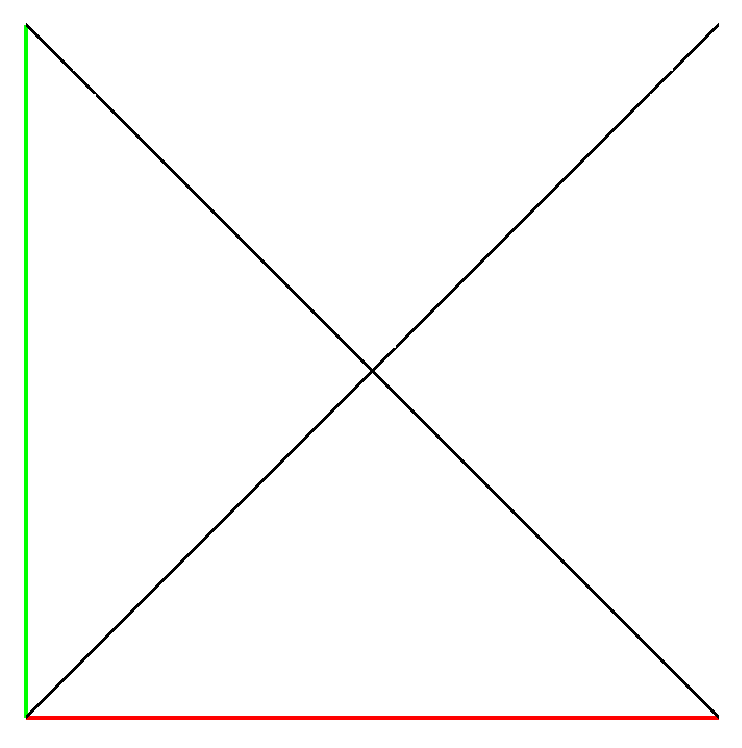
\includegraphics[height=0.25\linewidth,width=0.25\linewidth]{chapter-03/figs/bernstein1}%
   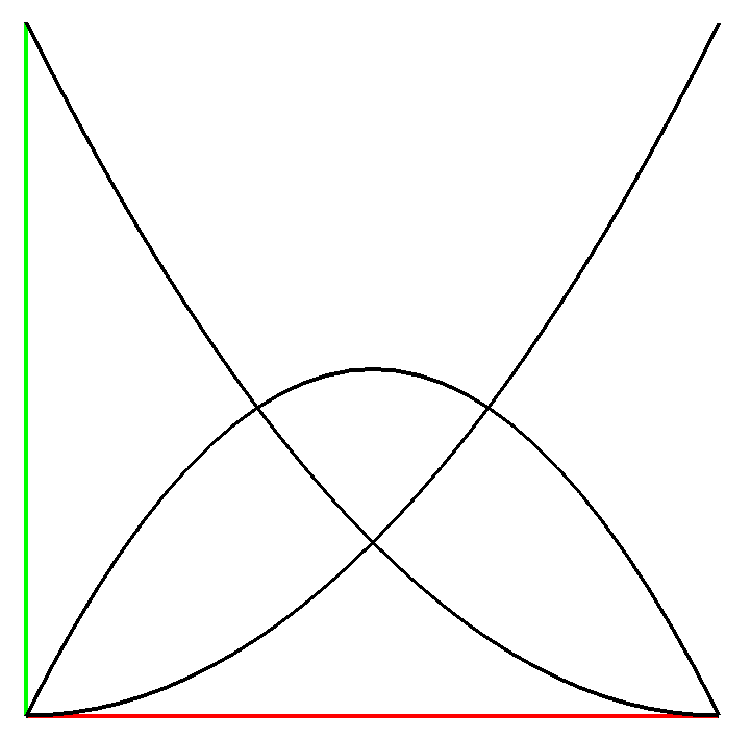
\includegraphics[height=0.25\linewidth,width=0.25\linewidth]{chapter-03/figs/bernstein3}%
   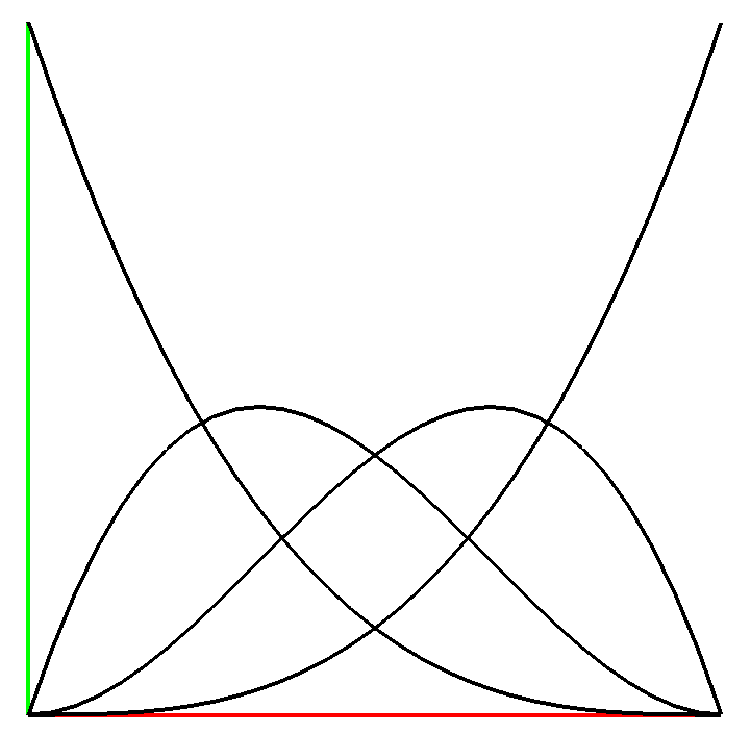
\includegraphics[height=0.25\linewidth,width=0.25\linewidth]{chapter-03/figs/bernstein2}%
   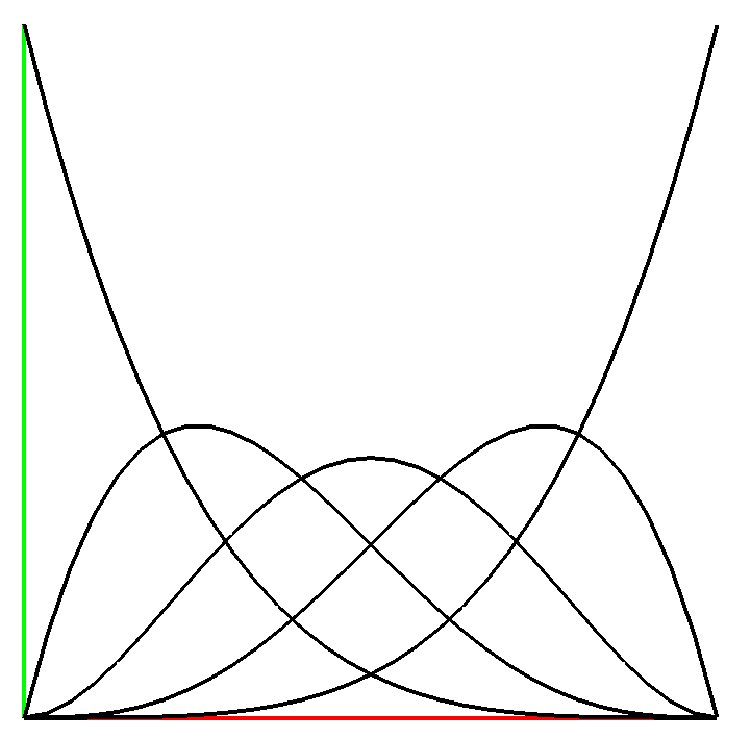
\includegraphics[height=0.25\linewidth,width=0.25\linewidth]{chapter-03/figs/bernstein4}%
   \caption{The four images give the graph, in $[0,1]\times[0,1]\subset\mathbb{E}^2,$ of Bernstein’s basis of linear, quadratic, cubic, and quartic polynomials in linear spaces $ 
   \P_n(\R)$, with $1\leq n\leq 4$, and $\dim(\P_n(\R)) = n+1 = {}$2, 3, 4, and 5, respectively.}
   \label{fig:bernstein}
\end{figure}  


\begin{coding}[Example of \texttt{FL \& Plasm} Combinators]
We remark on the incredible expressive power of |FL| programming inherited in |Plasm.jl|.

It is greatly useful to analyze goals and types of subexpressions, recuperating backward the development process to  write the result expression.
First, we define the 1D model |dom1D| of the function domain $[0,1]$ with 36 intervals, which is a geometric value of |Hpc| type:

\begin{lstlisting}[language=JuliaLocal, style=julia]
dom1D = INTERVALS(1.0)(36)  	#=
Hpc(MatrixNd([[1.0, 0.0], [0.0, 1.0]]), BuildMkPol[BuildMkPol(points=[[0.0], [0.027777777777777776], ... =#
\end{lstlisting}

Then, consider the $\E\to\E^2$ vector function |CONS(...)∘S1| of one variable, that is applied to the vertices of |dom1D::Hpc| by the |MAP| operator. 

The selector function |S1| is used to extract the first (and unique) coordinate value from the internal data structure |point| array. The |CONS| operator, acting on argument of |Vector{Function}| type, transforms a  function array into a vectorial function of coordinate functions |x(u)|, |y(u)|, etc. 

Hence, we have |F = CONS(::Vector{Function})∘Sd|${} : \E^d\to\E^n$, where |d| is the number of coordinates of domain vertices (one in this case), and |n| is the dimension of the embedding space, i.e., the number of coordinate functions inside the array argument, i.e.~|CONS([,])|, two in this case:

\begin{lstlisting}[language=JuliaLocal, style=julia]
F(k) = CONS([ID, Bernstein(4)[k]])∘S1		#=
#122 (generic function with 1 method)	=#
\end{lstlisting}

Finally, we note that expressions like |MAP(F)(dom1D)| are used to apply the |F| vector function to an object of |Hpc| type, normally to bend it.
Remember that we  generated an array of |Hpc| curves, for |k=1:n+1| --- in our case with |n=4|. For this purpose, we need to finally apply the |STRUCT| operator, to transform the array of curves into a single |Hpc| value.
\begin{lstlisting}[language=JuliaLocal, style=julia]
STRUCT( MAP(F(k))(dom1D) for k=1:n+1 )
\end{lstlisting}

\end{coding}


\subsubsection*{Change of basis} 

It is often necessary, given a basis in a linear space, to compute a novel parameterization of the space with respect to a different, possibly more simple or useful basis. In other words, may be necessary to compute new coordinates for the vectors of the space, with respect to a new basis. This operation is called \emph{change of basis}. 

For concreteness, let we have vector data in a 3D linear space, where we need to compute their representation in a different basis. Let us denote the new basis as $(\v{u}_i)$, and the standard one as $(\v{e}_i)$, with $i\in \{1,2,3\}$. We may write the change of coordinates as a matrix map $\T{T}: \mathcal{V}\to\mathcal{V}$, such that $[u_{ij}] \mapsto [e_{ij}]$, so transforming the old coordinates of the new basis into the standard basis. 

Therefore we set $\T{T}\, [u_{ij}] = [e_{ij}]$ and, since it is $[e_{ij}]=\mathbb{I}_{3}$, i.e., the $3\times 3$ identity matrix, the solution is $\T{T}=[u_{ij}]^{-1}$. Of course, this matrix exists provided that $\det\, [u_{ij}] \not= 0$. In other words, the vectors of the new basis must be linearly independent.


\subsection{Affine space}
\label{subsec:2:style}

In geometric modeling and computer graphics it is useful to distinguish between a space of vectors and a space of points (supported by vectors). A space of points, that provides for an operation of \emph{displacement}, is called an \emph{affine space}, and is represented here by the $\mathcal{A}$ symbol. In particular, we call \emph{affine action}  the function:
\[
\mathcal{A} \times \mathcal{V} \to \mathcal{A},
\]
so that  the \emph{displacement} from a point $\p{a} \in \mathcal{A}$ to a point $\p{b} \in \mathcal{A}$ is given. An affine space $\mathcal{A}$ is endowed with an operation of \emph{difference} of points $\mathcal{A} \times \mathcal{A} \to \mathcal{V}$ where
\[
\p{a} + \v{v} = \p{b}, \quad\mbox{and hence}\quad \p{b}-\p{a} = \p{v} \in \mathcal{V} 
\]

\subsubsection*{Remarks}
\label{sec:ccccccc}

We note that a \textbf{vector space} provides   for an internal operation of (a) \emph{sum} of two vectors and the external (b) \emph{product} of a vector by a scalar, both returning a vector. Conversely, in an \textbf{affine space} we have an external operation of (i) \emph{difference} of points, returning a vector, and  a (ii) sum of a point and a vector, called \emph{displacement}, returning a point.

Even more, in a vector space $\mathcal{V}$ there is a distinguished element $0$, the \emph{zero vector}, which is contained in all subspaces. On the contrary, in an affine space $\mathcal{A}$ \emph{all points are equivalent}, with no distinguished elements. 

We usually say that a space of points has been parameterized when a \emph{Cartesian system} (origin and basis) has been chosen.
In order to use coordinates to make it easier to work with points we have to choose :

\begin{enumerate}
\item 
a point, called \emph{origin}, to associate with the zero vector, and 
\item 
an orthonormal \emph{basis} of vectors. 
\end{enumerate}

The above steps consent to associate each point with the tuple of coordinates of its \emph{displacement vector} from the origin. 

In a vector space all the subspaces have at least a common element, the zero vector. Contrariwise, two affine subspaces may not have common elements. In such a case they are said \emph{parallel}. 

The dimension $n$ of an affine space $\mathcal{A}$ is that of its supporting vector space $\mathcal{V}$.
A common word for \emph{affine subspaces} of $d$ dimension is $d$-hyperplane, or $d$-hyperspace when $d>3$. Lines and planes are affine subspaces of dimension $1$ and $2$, respectively. 


\subsubsection*{Affine independence and local parameterization}
\label{sec:ccccccc}

In an affine space $\mathcal{A}$ of sufficiently high dimension $n$ we say that two points are \emph{affinely independent} when \emph{non coincident}, three points when \emph{non aligned}, four points when \emph{non coplanar}, and so on. 

In general, $d+1$ points  ($d \leq n$) are affinely independent when the $d$ vectors defined by the differences $\p{p}_k - \p{p}_0$ of points from one of them are linearly independent. 

The affine independence of a subset of $d+1$ points is often used to establish \emph{local coordinate systems} on lines, planes and higher dimensional subsets of points. Let us choose two non coincident points $\p{a},\p{b}$ on a 3D line. Any other point $\p{p}$ of the line remains parameterized by the $\alpha$ scalar in the expression 
\[
\p{p} = \p{a} + \alpha(\p{b}-\p{a}). 
\]
Note that $\p{b}-\p{a}$ is a vector, $\alpha(\p{b}-\p{a})$ is a vector, $\p{a} + \alpha(\p{b}-\p{a})$ is a point plus a vector, which is a point. The typing of our expression looks correct!

Analogously, let us choose three non colinear points $\p{a},\p{b},\p{c}$ in 3D space. They are certainly non coincident, and of course fix a plane, i.e., an unique affine subspace of dimension 2 embedded in space. A parameterization of this plane is given by the pairs $(\alpha,\beta)$ of scalars in the expression
\[
\p{q} = \alpha(\p{b}-\p{a}) + \beta(\p{c}-\p{a}),
\] 
as the reader may immediately check. Similar local coordinates will hold in every affine $d$-subspace in $n$-dimensional space.

The typical affine space of points used in this book is the Euclidean space $\mathbb{E}^d$, $1 \leq d \leq 3$, usually furnished of a Cartesian system, with coordinates in |Float64|.



\subsection{Convex space}
\label{subsec:2:style}

Let us consider the Euclidean space $\mathbb{E}^d$, $d\in\{2,3\}$ affine over the reals, that is the fundamental space of geometry, intended to represent physical space. 

Affine subspaces become \emph{convex sets} when a numeric constraint is imposed on the possible parameter values of an affine combination of points. Two points $\p{a},\p{b}\in\mathcal{A}$ become the extreme elements of a \emph{line segment} $\p{p} = \alpha\,\p{a} + (1-\alpha)\,\p{b}$ as set of points, by adding the further constraint $\alpha + \beta=1$ to the parameter values $\alpha,\beta \geq 0$, so posing $\beta=1-\alpha$. Analogously, setting $\alpha + \beta + \gamma = 1$ and $\alpha, \beta, \gamma \geq 0$ constraints the set of points combination of three non aligned points $(\p{a}, \p{b}, \p{c})$. 


\subsubsection*{Positive, Affine and Convex Combination of Points}
\label{par:AffineConvexCombination}

Let $\p{p}_1, \p{p}_2, \ldots, \p{p}_n$ be affinely independent points in $\mathbb{E}^d$, and $\alpha_1, \alpha_2, \ldots, \alpha_n$ be scalar in $\mathbb{R}$. Their combination $\alpha_1 \p{p}_1 + \alpha_2 \p{p}_2 + \cdots + \alpha_n \p{p}_n$ is said \emph{positive}, \emph{affine}, and \emph{convex}, respectively, when
\begin{enumerate}
\item $\alpha_1, \alpha_2, \ldots, \alpha_n \geq 0$ \hfill (positive combination)
\item $\alpha_1 + \alpha_2 + \cdots + \alpha_n = 1$ \hfill (affine combination)
\item $\alpha_1 + \alpha_2 + \cdots + \alpha_n = 1\quad\mbox{and}\quad \alpha_1, \alpha_2, \ldots, \alpha_n \geq 0$ \hfill (convex combination)
\end{enumerate}

It may be interesting to verify that the affine combination of points is a point.
Let us eliminate the $\alpha_1$ scalar using the unitary sum of scalars constraint:
\begin{eqnarray}
\p{p} = (1 - \alpha_2 - \cdots - \alpha_n) \p{p}_1 + \alpha_2 \p{p}_2 + \cdots + \alpha_n \p{p}_n\\
= \p{p}_1 + \alpha_2 (\p{p}_2-\p{p}_1) + \cdots + \alpha_n (\p{p}_n-\p{p}_1)
\end{eqnarray}
which, of course, is a point in $\mathbb{E}^d$.

A convex combination is positive and affine.

The set of all convex combinations of points $C \subset \mathbb{E}^n$ is the \emph{convex hull} of $C$.  The convex hull is the smallest compact set containing the points in $C$.
It is the intersection of all compact sets of $\mathbb{E}^d$ which contain $\mbox{hull}\, C$. 

\emph{Convex coordinates} of a point $\p{c} \in \mbox{hull}\, C$ are the scalars whose convex combination with $C$ elements produces $\p{c}$. If $C\subset \mathcc{E}^n$ has $n+1$ affinely independent elements, i.e., it is a simplex (see Section \ref{sec:simplex}) the convex coordinates of each $\p{c} \in \mbox{hull\ } C$ are \emph{unique}.


\subsubsection*{Characterization of affine pyramids}
\label{sec:ccccccc}

Speaking of local parameterization of affine subspaces, we did not fix any constraint on the signs of the scalar parameters (usually in the field $\mathbb{R}$ of reals). If all the scalars are positive, then all the spanned points stay inside the interior of a planar (or solid) angle contained within the lower-dimensional affine subspaces generated. It would be not difficult to see that the whole subspace will be partitioned by an arrangement of subspaces centered on the fixed point of the set of linearly independent vectors. As an example, consider the partitioning of 3D space generated by the $8 = 2^3$ octants defined by $4$ non coplanar points, and in particular those generated when three points are at unit distance by the first, and the three difference vectors are pairwise orthogonal.

\subsubsection*{Positive, Affine and Convex coordinates}

%12345678901234567890123456789012345678901234567890123456789012345678901234567890

Affine Coordinates for Convex Sets

Barycentric Coordinates for Convex Sets

Test for boundary points: interior and exterior









\section{Cellular models}\label{sect:3-2}


This section discusses computational topology concepts used to compute the 2D/3D space partition induced by a collection of geometric objects of dimension 1D/2D, respectively. Cellular models are are often called \emph{meshes} in engineering and design jargon. A mesh is a representation of a domain by discrete cells. In many areas of geometric/numeric computational engineering, including geo-mapping, computer vision and graphics, finite element analysis, medical imaging, geometric design, and solid modeling, one has to compute incidences, adjacencies and ordering of mesh cells, generally using disparate and incompatible data structures and algorithms. Only sparse vectors and matrices are used in |Plasm| to compute the linear spaces of chains, called chain complex, from dimension zero to three.

\subsection*{Topological definitions}\label{sect:3-2-1}

A \emph{complex} is a graded set $S = \{ S_i \}_{i\in I}$ \emph{i.e.}~a family of sets, indexed here over $I = \{0,1,2,3\}$.
We use two different but intertwined types of {complexes}, and specifically complexes of \emph{cells} and complexes of \emph{chains}. 
Their definitions and some related concepts are given in this section. Greek letters are used for the {cells} of a space partition, and roman letters for {chains} of cells, coded as either (un)signed integers or sparse arrays of (un)signed integers.  


\begin{definition}[$d$-Manifold]
A \emph{manifold} is a topological space that resembles a flat space locally, \emph{i.e.}, near every point. 
Each point of a $d$-dimensional manifold has a neighborhood that is homeomorphic\footnote{Homeomorphic means opologically equivalent.} to $\E^d$, the Euclidean space of dimension $d$. Hence, this geometric object is often referred to as $d$-manifold. 
\end{definition}
\emp{Homeomorphic} neighborhood means “topologically equivalent”, like a rubber patch, that can be stretched without changing its topology.
%\end{paragraph}

\begin{definition}[Cell]
A \emph{$p$-cell} $\sigma$ is a $p$-manifold with boundary ($0\leq p\leq d$) which is 
piecewise-linear, connected, possibly non convex, and not necessarily contractible. This definition refers to cellular complexes used in this paper and is different from other ones because a cell is neither simplicial, nor convex, nor contractible.
\end{definition}
In |Plasm|, cells may contain internal holes; cells of CW-complexes~\cite{hatcher:2002} are, conversely,  contractible to a point.  
We deal with \emph{Piecewise-Linear} (PL) cells of dimensions 0, 1, 2, and 3, respectively. It should be noted that 2- and 3-cells may contain holes, while remaining connected.  In other words, |Plasm| cells are $p$-polyhedra, \emph{i.e.}~segments, polygons and polyhedrons embedded in 2D or 3D space. 
%%\end{definition}

\begin{definition}[Cellular complex]
A \emph{cellular $p$-complex} is a finite set of cells that have at most dimension $p$, together with all their $r$-dimensional boundary faces ($0\leq r\leq p$). A \emph{face} is an element of the PL boundary of a cell, that satisfy the \emph{boundary compatibility} condition. Two $p$-cells $\alpha, \beta$ are said boundary-compatible when their point-set intersection contains the same $r$-faces ($0\leq r\leq p$) for both $\alpha$ and $\beta$. 
\end{definition}
A cellular $p$-complex is said {\emph{homogeneous} }when each $r$-cell ($0\leq r\leq p$) is face of a $p$-cell. 

\begin{definition}[Skeleton]
The $s$-skeleton of a $p$-complex $\Lambda_p$ ($s\leq p$) is the set $\Lambda_s\subseteq\Lambda_p$ of all $r$-cells ($r\leq s$) of $\Lambda_p$. Every skeleton of a regular complex is a regular subcomplex.
The difference $\Lambda_r - \Lambda_{r-1}$ of two skeletons is the set $U_r$ of $r$-cells. 
\end{definition}

\begin{definition}[Support space]
The support space $\Lambda$ of a cellular complex is the point-set union of its cells. 
\end{definition}

\begin{definition}[Characteristic function]
Given a subset $S$ of a larger set $A$, the characteristic function $\chi_A(S)$, also called the \emph{indicator function}, is the function defined to be identically one on $S$, and zero elsewhere. \cite{Wolfram}.
\end{definition}


\subsection{Simplicial complex}\label{sect:3-2-1}


\begin{definition}[Join operation.]
\index{Simplex}
The {\em join} of two compact sets of points $P,Q\subset\E^n$ is the set $PQ$ of convex combinations of points in $P$  and in $Q$.
The join operation is associative and commutative.  
\end{definition}


\begin{definition}[Simplex.]
A {\em $d$-simplex} $\sigma_{d}\subset \E^n$ ($0\leq d\leq n$) may be
defined as the repeated join of $d+1$ affinely independent points,
called {\em vertices}.  
\end{definition}
A $d$-simplex can be seen as a $d$-dimensional
triangle: a $0$-simplex is a \emph{point}, a $1$-simplex is a
\emph{segment}, a $2$-simplex is a \emph{triangle}, a $3$-simplex is a
\emph{tetrahedron}, and so on.


\begin{coding}[Plasm $d$-dimensional simplex]  A $d$-simplex is generated by the |Plasm| package by the |SIMPLEX| multi-dimensional function:
\begin{lstlisting}[language=JuliaLocal, style=julia, mathescape = true] 
julia> using Plasm

julia> SIMPLEX::Function
SIMPLEX (generic function with 1 method)
\end{lstlisting}
\end{coding}


\begin{coding}[Dataset associated to simplices.] The simplex datasets follow, for the first integer parameters. Note that |SIMPLEX(d)| contain $d+1$ coordinate points of dimension $d$, and that |hulls| fields contain $d+1$ indices of points, i.e. a single \emph{convex} cell:
\begin{lstlisting}[language=JuliaLocal, style=julia, mathescape = true]
SIMPLEX(0)			#=
Hpc(MatrixNd(1), Geometry([Float64[]], hulls=[[1]])) =#

SIMPLEX(1)			#=
Hpc(MatrixNd(2), Geometry([[0.0], [1.0]], hulls=[[1, 2]])) =#

SIMPLEX(2)			#=
Hpc(MatrixNd(3), Geometry([[0.0, 0.0], [1.0, 0.0], [0.0, 1.0]], hulls=[[1, 2, 3]])) =#

SIMPLEX(3)			#=
Hpc(MatrixNd(4), Geometry([[0.0, 0.0, 0.0], [1.0, 0.0, 0.0], [0.0, 1.0, 0.0], [0.0, 0.0, 1.0]], hulls=[[1, 2, 3, 4]])) =#

SIMPLEX(4)			#=
Hpc(MatrixNd(5), Geometry([[0.0, 0.0, 0.0, 0.0], [1.0, 0.0, 0.0, 0.0], [0.0, 1.0, 0.0, 0.0], [0.0, 0.0, 1.0, 0.0], [0.0, 0.0, 0.0, 1.0]], hulls=[[1, 2, 3, 4, 5]])) =#
\end{lstlisting}
\end{coding}

For the sake of visual simplicity, we remove the |julia>| prompt for Plasm scripts, and use the multilinear comment to reduce their visual rumor.


\begin{definition}\emph{Skeleton and Faces.}
The set $\{ \p{v}_0, \p{v}_1, \ldots, \p{v}_d \}$ of vertices of
$\sigma_{d}$ is called the {\em 0-skeleton} of $\sigma_{d}$.  The
$s$-simplex generated from {\em any} subset of $s+1$ vertices ($0\leq
s\leq n$) of $\sigma_{d}$ is called an {\em $s$-face} of $\sigma_{d}$.
\end{definition}
\begin{remark}
Let us notice, from the definition, that a simplex may be considered
both as a purely \emph{combinatorial object} and as a \emph{geometric object}, i.e.
as the compact point-set defined by the convex hull of a discrete set
of points.
\end{remark}


\begin{definition}[Simplicial Complex]
A set $\Sigma$ of simplices is called a {\em triangulation}.  
A {\em simplicial complex}, often simply denoted as \emph{complex}, is
a triangulation $\Sigma$ that verifies the following conditions:
\begin{enumerate}
\item
if $\sigma \in \Sigma$, then any face of $\sigma$ belongs to $\Sigma$;

\item
if $\sigma,\tau\in \Sigma$, then either $\sigma\cap
\tau=\emptyset$, or $\sigma\cap\tau$ is a face of both $\sigma$ and
$\tau$.
\end{enumerate}
\end{definition}

A simplicial complex can be considered a \emph{well-formed}
triangulation.  Such kind of triangulations are widely used in
engineering analysis, e.g., in topography or in finite element
methods.

\begin{coding}[binomial numbers and simplex faces]
There are 
\[
\sum_{k=0}^{n} {n \choose k} = 2^n
\] 
$k$-faces in a $n$-simplex. Testing this statement is simple and very elegant with Julia. 
We may verify, e.g., that |simplex(5)| faces are a set of |$2^5$| elements:
\begin{lstlisting}[language=JuliaLocal, style=julia, mathescape = true]
julia> [binomial(5,k) for k=0:5]'
1×6 adjoint(::Vector{Int64}) with eltype Int64:
 1  5  10  10  5  1

julia> [binomial(5,k) for k=0:5] |> sum == 2^5
true
\end{lstlisting}


\end{coding}

\begin{coding}
A simple coding example produces the simplicial complex providing the triangulation of the boundary of a convex hull. 
\begin{lstlisting}[language=JuliaLocal, style=julia, mathescape = true]
julia> p = rand(6,3)				#=
6×3 Matrix{Float64}:
 0.456121  0.340689  0.523394
 0.670731  0.920846  0.810581
 0.511325  0.83709   0.765548
 0.27295   0.344676  0.246891
 0.155611  0.262588  0.372059
 0.997037  0.689132  0.594624		  =#
\end{lstlisting}
The |p| matrix holds 6 random |3D| points. The |q| matrix receives an array of arrays:
\begin{lstlisting}[language=JuliaLocal, style=julia, mathescape = true]
julia> q = [p[k,:] for k=1:size(p,1)]				#=
6-element Vector{Vector{Float64}}:
 [0.4561213293752391, 0.34068894716553066, 0.5233939444809501]
 [0.6707310911896536, 0.9208461259235498, 0.8105811405026019]
 [0.5113250218604997, 0.8370897242704682, 0.7655476328700838]
 [0.2729499977250678, 0.3446764528053594, 0.24689130455109154]
 [0.15561059083290985, 0.26258788197490757, 0.37205895443742]
 [0.9970371401112009, 0.6891321979374976, 0.5946242627157257]  =#
\end{lstlisting}
Their convex hull is computed by the |Plasm| function |CONVEXHULL| and stored as |Hpc| data structure:
\begin{lstlisting}[language=JuliaLocal, style=julia, mathescape = true]
julia> CONVEXHULL(q)				#=
Hpc(MatrixNd(4), Geometry([[0.4561213293752391, 0.34068894716553066, 0.5233939444809501], [0.6707310911896536, 0.9208461259235498, 0.8105811405026019], [0.5113250218604997, 0.8370897242704682, 0.7655476328700838], [0.2729499977250678, 0.3446764528053594, 0.24689130455109154], [0.15561059083290985, 0.26258788197490757, 0.37205895443742], [0.9970371401112009, 0.6891321979374976, 0.5946242627157257]], hulls=[[1, 2, 3, 4, 5, 6]]))				=#
\end{lstlisting}
And finally the dataset is transformed into a |Lar| data structure, which contains all the boundary polygons |:FV| and edges |:EV|.
\begin{lstlisting}[language=JuliaLocal, style=julia, mathescape = true]
julia> LAR(CONVEXHULL(q)) 				#=
Lar(3, 3, 6, [0.27294999772507 0.67073109118965 … 0.15561059083291 0.5113250218605; 0.34467645280536 0.92084612592355 … 0.26258788197491 0.83708972427047; 0.24689130455109 0.8105811405026 … 0.37205895443742 0.76554763287008], Dict{Symbol, AbstractArray}(:CV => [[1, 2, 3, 4, 5, 6]], :FV => [[1, 2, 3], [2, 3, 4], [1, 4, 5], [1, 3, 4], [1, 5, 6], [1, 2, 6], [4, 5, 6], [2, 4, 6]], :EV => [[2, 3], [1, 3], [1, 2], [3, 4], [2, 4], [1, 4], [4, 5], [1, 5], [5, 6], [1, 6], [2, 6], [4, 6]])) 				=#
\end{lstlisting}
We remark that the |Hpc| describes only the \emph{convex cells} of its dataset. 
Conversely, the |Lar| data structure gives explicitly all cells of any dimension. 
\end{coding}



The {\em order} of a complex is the maximum order of its simplices.  A 
complex $\Sigma_{d}$ of order $d$ is also called a {\em $d$-complex}.  
A $d$-complex is said to be {\em regular} or {\em pure} if each 
simplex is a face of a $d$-simplex. A regular $d$-complex is 
homogeneously $d$-dimensional.
 
The \emph{combinatorial boundary} $\Sigma_{d-1} = \partial\sigma_{d}$
of a simplex $\sigma_{d}$ is a simplicial complex consisting of all
proper $s$-faces ($s < d$) of $\sigma_{d}$.

Two simplices $\sigma$ and $\tau$ in a complex $\Sigma$ are
called {\em $s$-adjacent} if they have a common $s$-face.  Hereafter, when
we refer to adjacencies into a $d$-complex, we intend to refer to the
maximum order adjacencies, i.e. to $(d-1)$-adjacencies.  ${\cal K}_{s}$
$(s\leq d)$ denotes the set of $s$-faces of $\Sigma_{d}$.  


\subsubsection*{Simplex orientation}
The ordering of $0$-skeleton of a simplex implies an {\em 
orientation} of it.
\begin{definition}[Ordering of simplex vertices]
The simplex can be oriented according to the 
even or odd permutation class of its $0$-skeleton.   
\end{definition}
The two opposite 
orientation of a simplex will be denoted as $+\sigma$ and $-\sigma$. 

\begin{definition}[Coherent orientation]
Two simplices are {\em coherently oriented} when their common faces 
have opposite orientation.  A complex is {\em orientable} when all its 
simplices can be coherently oriented.
\end{definition}

It is assumed that: 
\begin{enumerate}
    
\item 
the two orientations of a simplex represent its relative
interior and exterior; 

\item
the two orientations of an orientable simplicial complex analogously
represent the relative interior and exterior of the complex,
respectively; 

\item
the boundary of a complex maintains the same orientation of the complex.
\end{enumerate}

The volume associated with an orientation of a simplex (or complex) is
positive, while the one associated with the opposite orientation has the
same absolute value and opposite sign.  It is assumed that the bounded
object has positive volume.  It is also assumed that either a minus
sign or a multiplying factor $-1$ denote a complementation, i.e. an
opposite orientation of the simplex, which can be explicitly obtained
by swapping two vertices in its ordered $0$-skeleton. For example:
\[
+ \sigma_{3} &=& \langle \v{v}_{0}, \v{v}_{1}, \v{v}_{2}, \v{v}_{3} \rangle,
\qquad
- \sigma_{3} &=& \langle \v{v}_{1}, \v{v}_{0}, \v{v}_{2}, \v{v}_{3} \rangle.
\]

\begin{figure}
\centering
   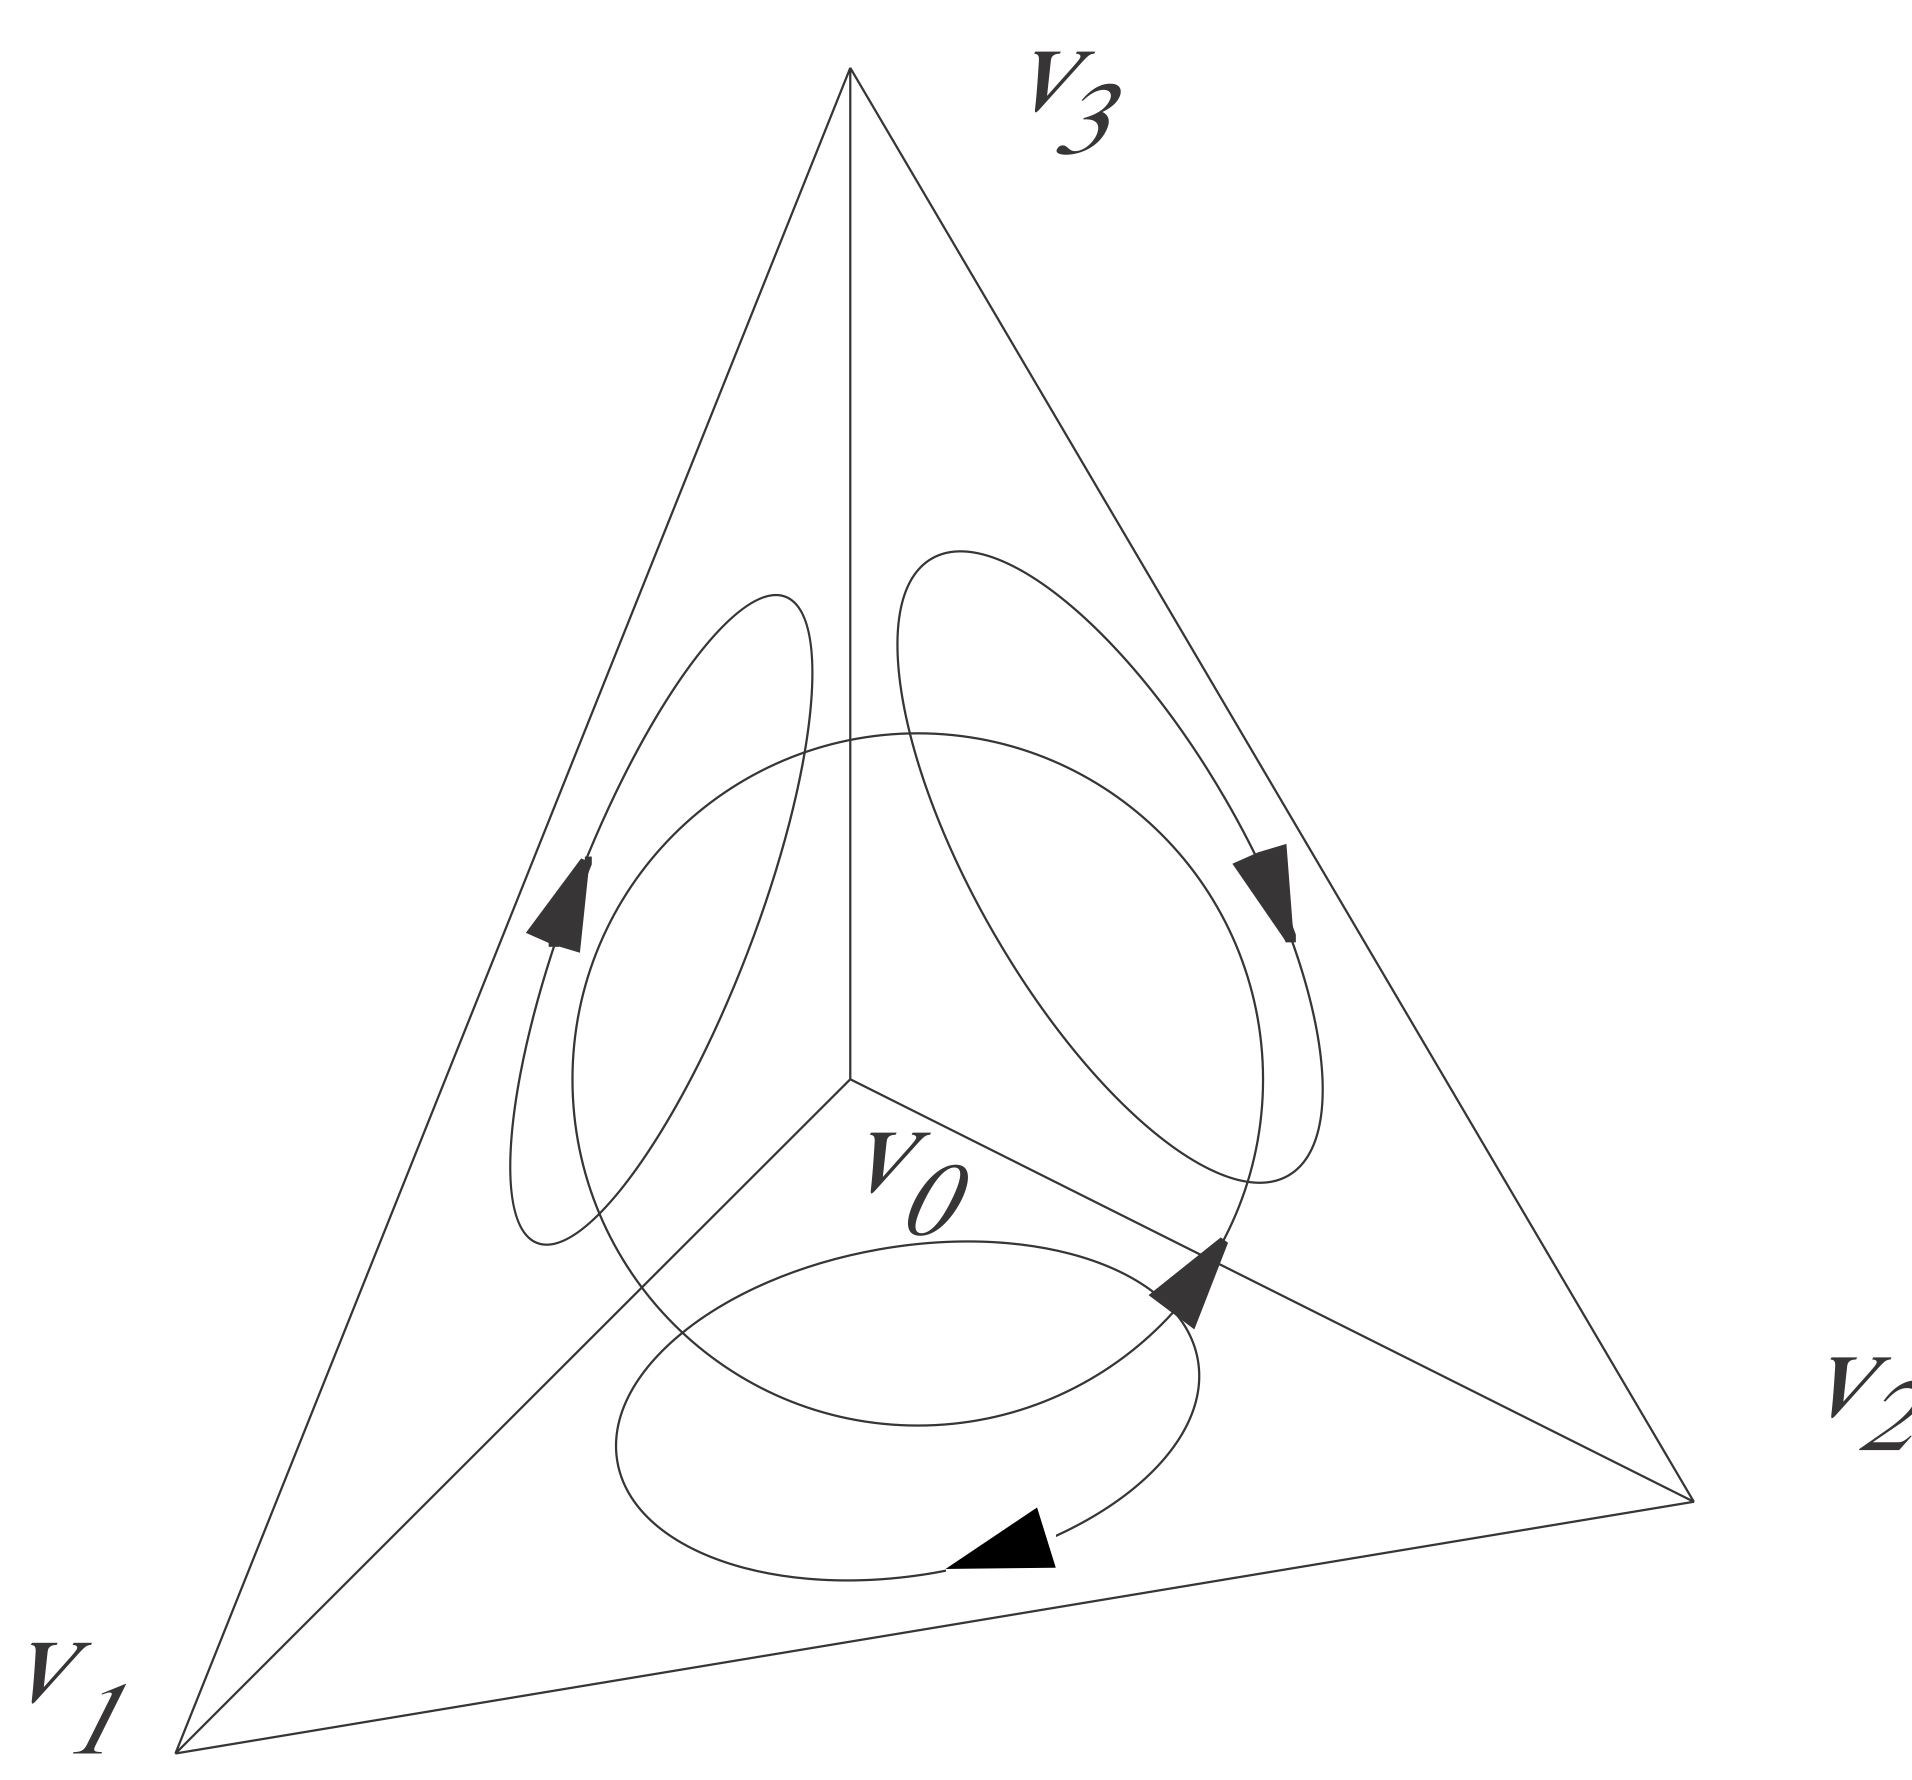
\includegraphics[width=2in]{chapter-03/figs/simplex0.png} \hfill~
\caption{Coherent orientation of the 2-faces of a 3-simplex}
\label{fig:6:simplex}
\end{figure}

\begin{definition}[Volume of a 3-simplex]\label{def:simplexvolume}
The volume of a 3-simplex is a 2-cochain (see Section \ref{sect:3-3}) from the cycle of its 2-faces (boundary triangles) to $\R$.  By definition, a 2-cochain is a map from 2-chains to $\R$.
\end{definition}



\subsubsection*{Facet extraction}\index{Faces!extraction}

The $(d-1)$-faces of a $d$-dimensional simplex or complex are also called \emph{facets} since no ambiguity may arise. It is possible to see \cite{Whitney:1957} what follows:

\begin{theorem}[Whitney, 1957]
The oriented facets $\sigma_{d-1}^{(i)}$ $(0\leq i\leq d)$ of the
oriented $d$-simplex $\sigma_d=+\langle \v{v}_0, \v{v}_1, \ldots,
\v{v}_d \rangle$ are obtained by removing the $i$-th vertex
$\v{v}_{i}$ from the $0$-skeleton of $\sigma_d$:
\begin{equation}
\sigma_{d-1}^{(i)}=(-1)^i(\sigma_d - \langle \v{v}_{i}\rangle), \qquad 0\leq 
i\leq d .
\label{eq:4:eq1}
\end{equation}
\end{theorem}
% where the minus sign denotes a subtraction between $0$-skeletons.

The $0$-skeleton of $\sigma_{d-1,(i)}$ is therefore obtained by removing the 
$i$-th vertex from the $0$-skeleton of $\sigma_{d}$ and either by swapping 
a pair of vertices or, better, by inverting the simplex sign, when $i$ 
is odd.  


\begin{coding}[Facets of a $d$-simplex.] A julia function is given here to compute combinatorially all the oriented facets of a |simplices| arrays of $d$-simplexes. A precondition is that all |Vector{Int64}| in the input sequence have the same length.
\lstinputlisting[language=JuliaLocal,style=julia,mathescape=false]{/Users/paoluzzi/Documents/dev/PLASM/SPRINGER/BOOK/chapter-06/src/009.jl}
If the |expr| after |@assert| is |false|, the program stops in |AssertionError:expr| 
\end{coding}

\begin{coding}[Execution example.] We can start from an array of simplices of the same length and iterate on their facets, to get a whole simplicial complex.
\begin{lstlisting}[language=JuliaLocal, style=julia, mathescape = true]
FV=[[123],[124],[134],[234]] #=
[[123],[124],[134],[234]] =#
EV = simplexfacets(FV)  #=
[[12],[13],[14],[23],[24],[34]] =#
VV = simplexFacets(EV)  #=
[[1], [2], [3], [4]]     =#
simplex(3,complex=true).C   #=
Dict(:c1v => EV, :c3v => [[1,2,3,4], :c0v => VV], :c2v => FV) =#
\end{lstlisting}
\end{coding}
We can also generate directly the whole bounday complex of a multidimensional simplex

\begin{coding}[Generation of boundary complex]\ 
We can olso directly generate the |Lar| boundary complex of a simplex of any degree:
\begin{lstlisting}[language=JuliaLocal, style=julia, mathescape = true]
simplex(4,complex=true).C			#=
Dict{Symbol, AbstractArray} with 5 entries:
  :C4V => [[1, 2, 3, 4, 5]]
  :C3V => [[1, 2, 3, 4], [1, 2, 3, 5], [1, 2, 4, 5], [1, 3, 4, 5], [2, 3, 4, 5]]
  :C0V => [[1], [2], [3], [4], [5]]
  :C2V => [[1, 2, 3], [1, 2, 4], [1, 2, 5], [1, 3, 4], [1, 3, 5], [1, 4, 5], [2…
  :C1V => [[1, 2], [1, 3], [1, 4], [1, 5], [2, 3], [2, 4], [2, 5], [3, 4], [3, …  =#
simplex(4,complex=true).V			#=
4×5 Matrix{Float64}:
 0.0  1.0  0.0  0.0  0.0
 0.0  0.0  1.0  0.0  0.0
 0.0  0.0  0.0  1.0  0.0
 0.0  0.0  0.0  0.0  1.0			 =#
\end{lstlisting}
\end{coding}


\begin{coding}[Simplex generation in \texttt{Hpc}]\ 
Convnersely, the |Plasm| data structure |Hpc| contains a single convex cell:
\begin{lstlisting}[language=JuliaLocal, style=julia, mathescape = true]
SIMPLEX(4)			#=
Hpc(MatrixNd(5), Geometry([[0.0, 0.0, 0.0, 0.0], [1.0, 0.0, 0.0, 0.0], [0.0, 1.0, 0.0, 0.0], [0.0, 0.0, 1.0, 0.0], [0.0, 0.0, 0.0, 1.0]], hulls=[[1, 2, 3, 4, 5]]))			 =#
\end{lstlisting}
\end{coding}

\begin{definition}[Simplicial extrusion]

The prism over a simplex $\sigma_{d} = \langle \p{v}_{0},\ldots,
\p{v}_{d} \rangle$, defined as the set $P_{d+1} := \sigma_{d} \times
[a,b]$, with $[a,b]\subset\E$, will be called \emph{simplicial $(d+1)$-prism}. 
An oriented complex which triangulates $P_{d+1}$ can be defined
combinatorially, by using a closed form formula for its ${\cal
K}_{d+1}$ skeleton:
\[
{\cal K}_{d+1} = \{ \sigma_{d+1,(i)} = (-1)^{id}
\langle \p{v}_{i}^{a},\p{v}_{i+1}^{a},\ldots,\p{v}_{d}^{a},
\p{v}_{0}^b,\p{v}_{1}^b,\ldots,\p{v}_{i}^b \rangle, \quad  0\leq i\leq d \}
\]
where $\p{v}_{i}^{a} = (\p{v}_{i},{a})$ and $\p{v}_{i}^{b} = 
(\p{v}_{i},{b})$.

Closed formulas to triangulate the $(d+1)$-prism over a $d$-complex in
a time linear with the size of the output, while computing also the
$d$-adjacencies between the resulting $(d+1)$-simplices, can be found
in~\cite{10.1016/0010-4485(91)90080-G,10.1145/164360.164376}.
\end{definition}


\subsection*{Simplicial grids}\index{Linear!d-Polyhedra}

In layout design, a grid system provides a framework of intersecting vertical and horizontal lines. Designers use this framework to place and align text, images, and other elements. 

Analogously, a \emph{simplicial grid}, is a geometric grid structure made by simplicial cells of same dimension aligned on a layout grid 1D, 2D, 3D, etc.
They are mainly used for domain decomposition, where to map coordinate functions in order to create curved structures, i.e., proper curves, curved surfaces, and curved solids.

The whole curved complex is easily generated by mapping the vertices of a |Lar| grid.


\begin{figure}[] %  figure placement: here, top, bottom, or page
   \centering   
   
\includegraphics[width=0.29\textwidth]{chapter-03/figs/extrude02.png}% 
   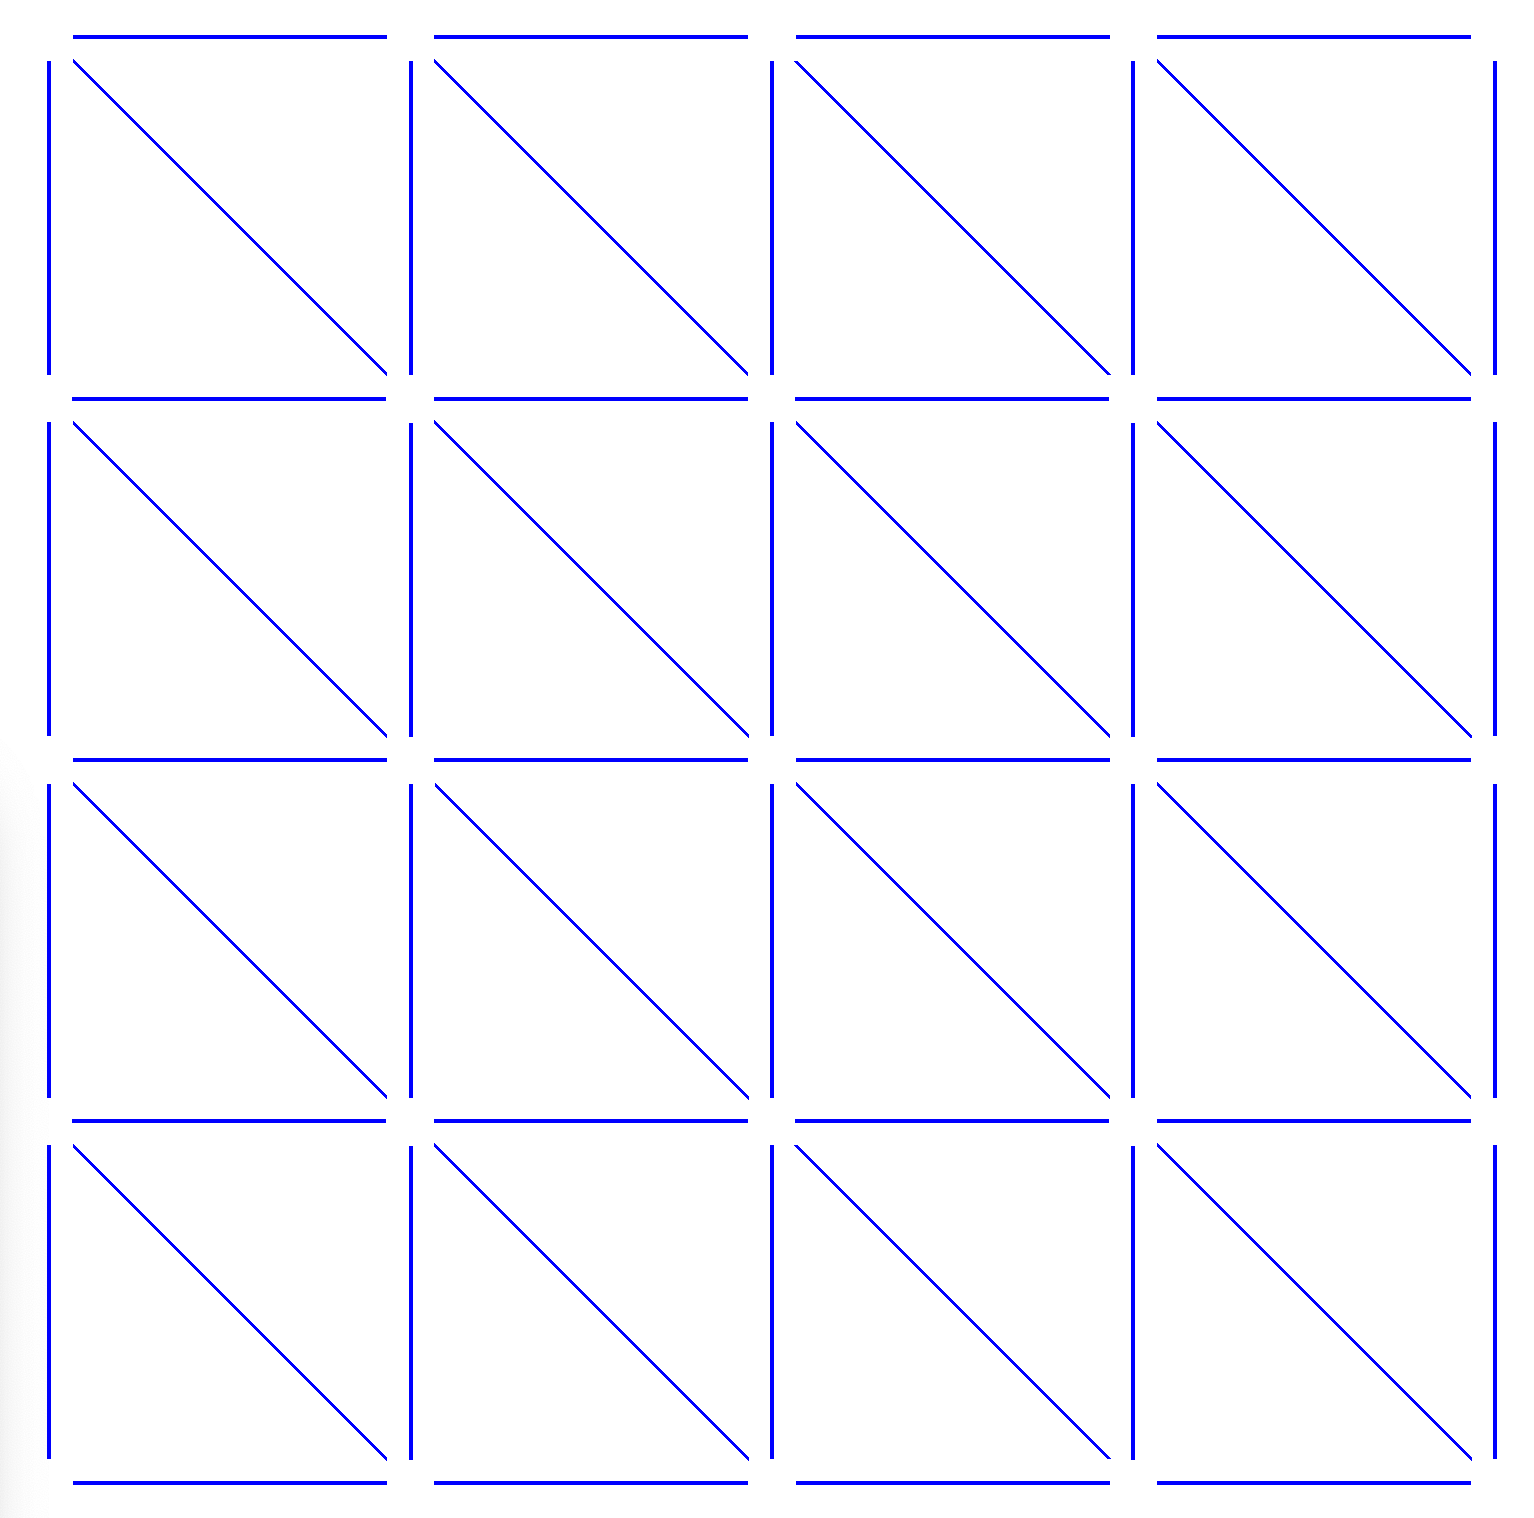
\includegraphics[width=0.29\textwidth]{chapter-03/figs/extrude03.png} 
   \caption{The simplicial 2- and 1-complex (shown here slightly exploded) are generated by \emph{extrudecomplex()} using the same pattern, both starting from \emph{model1D}.
   The 1-complex is derived by the 2-complex using \emph{simplexfacets()}.}
   \label{fig:3:extrude1}
\end{figure}

\begin{coding}[1D Extrusion]\ 
\begin{lstlisting}[language=JuliaLocal, style=julia, mathescape=false]
V1 = [ 0.0 1.0 2.0 3.0 4.0 5.0 ]
EV = [[1, 2], [2, 3], [3, 4], [4, 5]]
mod1D = Lar(V1, Dict(:c1v => EV))
V2 = [mod1D.V; zeros(size(mod1D.V,2))']
GL.VIEW(GL.GLExplode(V2, map(x->[x],EV),1.1,1.1,1.1,2,1));
\end{lstlisting}
\end{coding}

The |mod2D| and |mod3D| grids are generated by the following code.

\begin{coding}[2D Extrusion]\
\begin{lstlisting}[language=JuliaLocal, style=julia, mathescape=false]
mod2D = extrudecomplex(mod1D::Lar, [1, 1, 1, 1])
FV = collect(values(mod2D.C))[1]
EV = simplexfacets(FV)
GL.VIEW(GL.GLExplode(mod2D.V, map(x->[x],EV),1.2,1.2,1.2,4,1));
\end{lstlisting}
\end{coding}

\begin{coding}[3D Extrusion]\
\begin{lstlisting}[language=JuliaLocal, style=julia, mathescape=false]
mod3D = extrudecomplex(mod2D::Lar, [1,-2,1])
CV = collect(values(mod3D.C))[1]
FV = simplexfacets(CV)
EV = simplexfacets(FV)
GL.VIEW(GL.GLExplode(mod3D.V,map(x->[x],EV),2,2,2,99,1));
\end{lstlisting}
\end{coding}

\begin{figure}[] %  figure placement: here, top, bottom, or page
   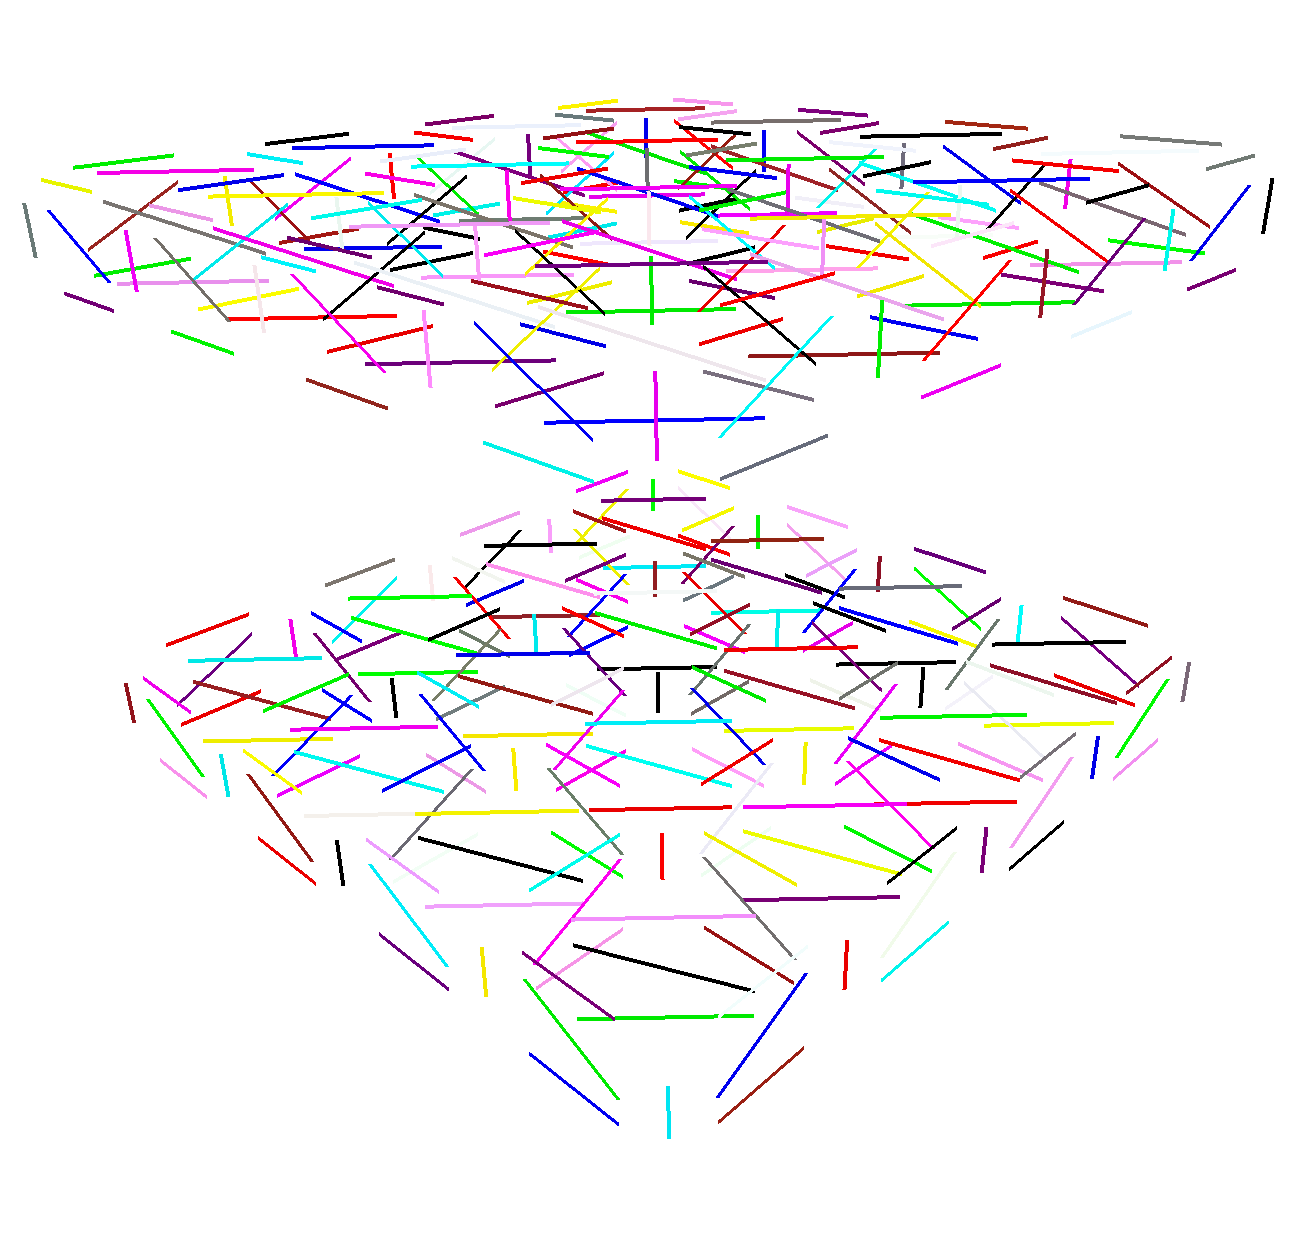
\includegraphics[eight=0.335\linewidth,width=0.33\linewidth]{chapter-03/figs/extrude06.png}%
   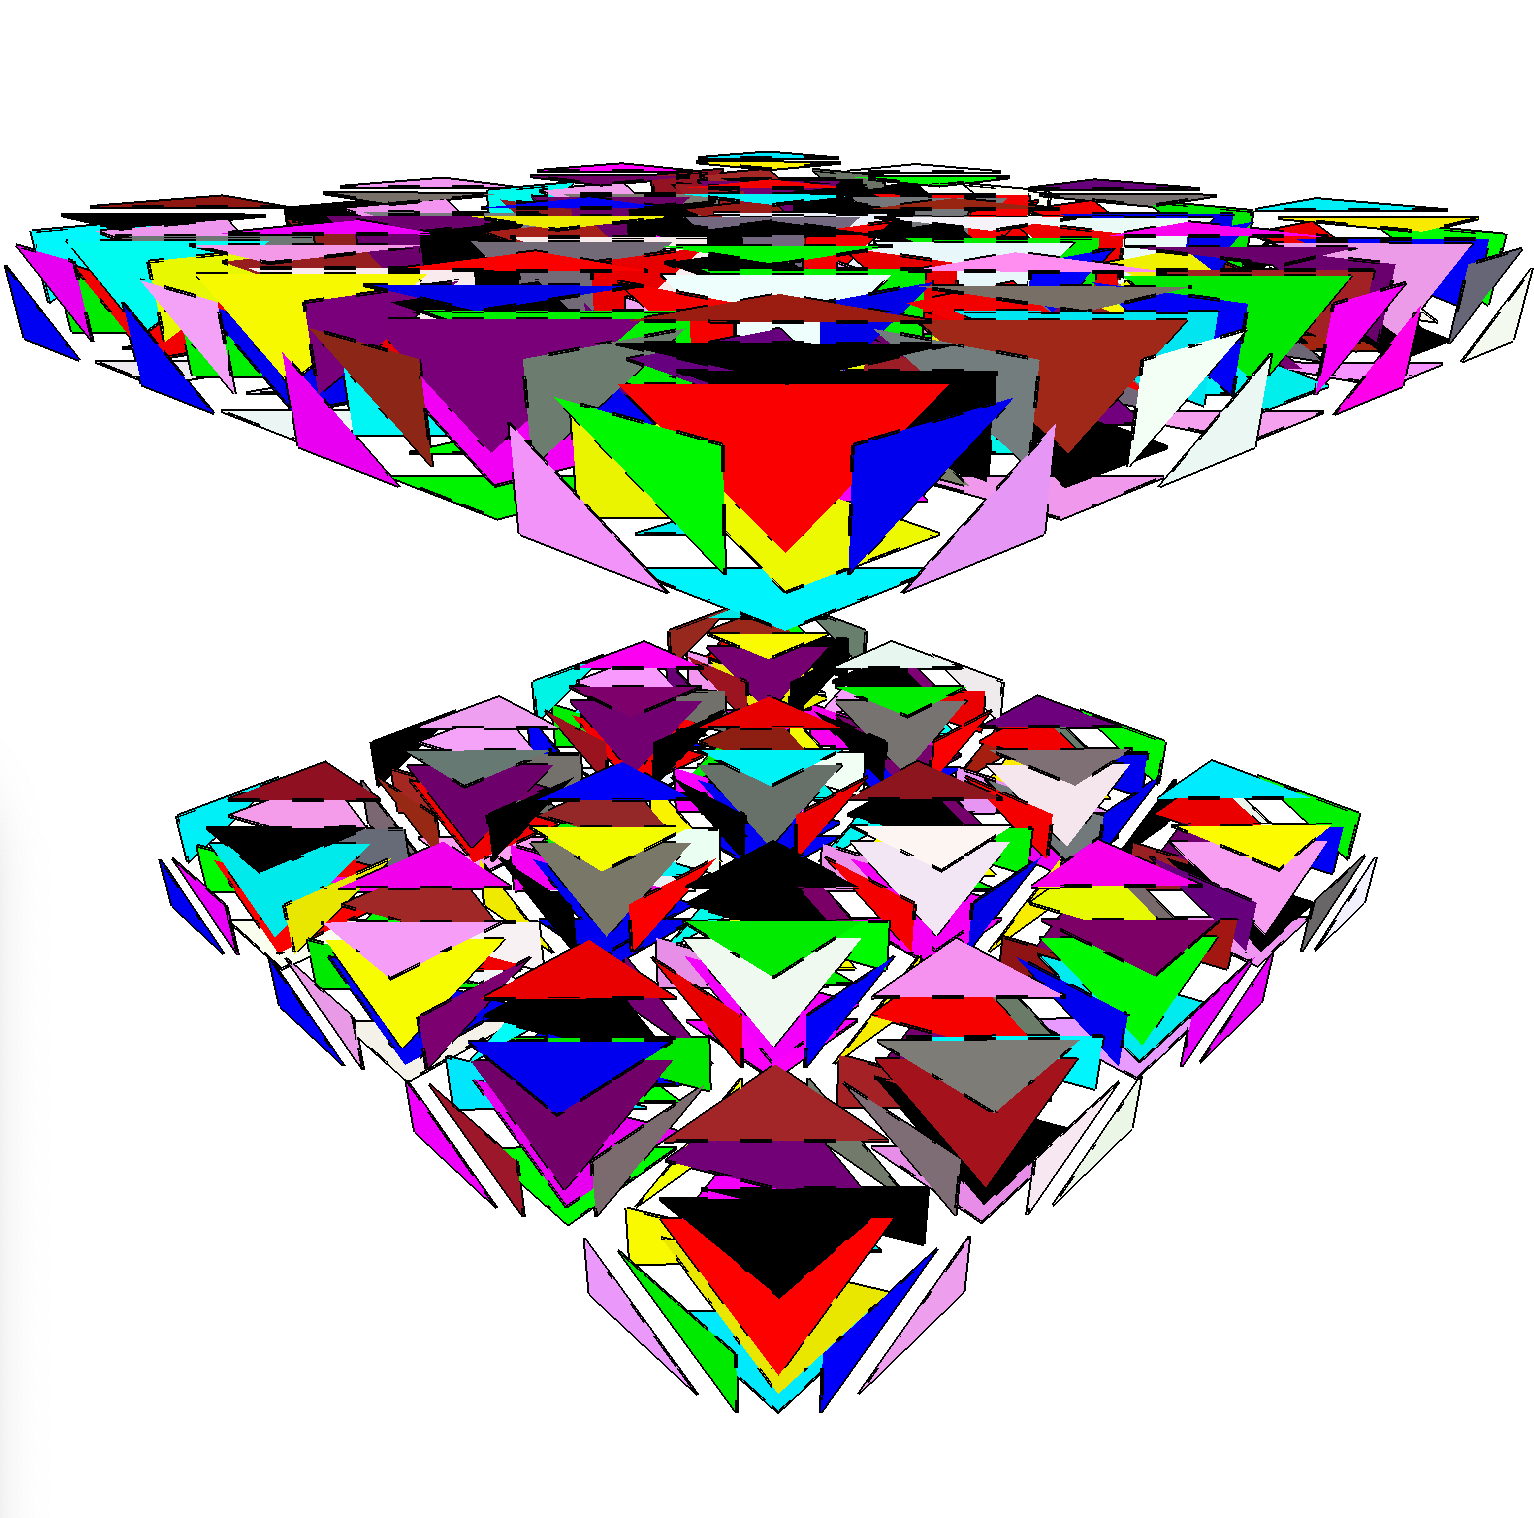
\includegraphics[eight=0.33\linewidth,width=0.33\linewidth]{chapter-03/figs/extrude04.png}%
   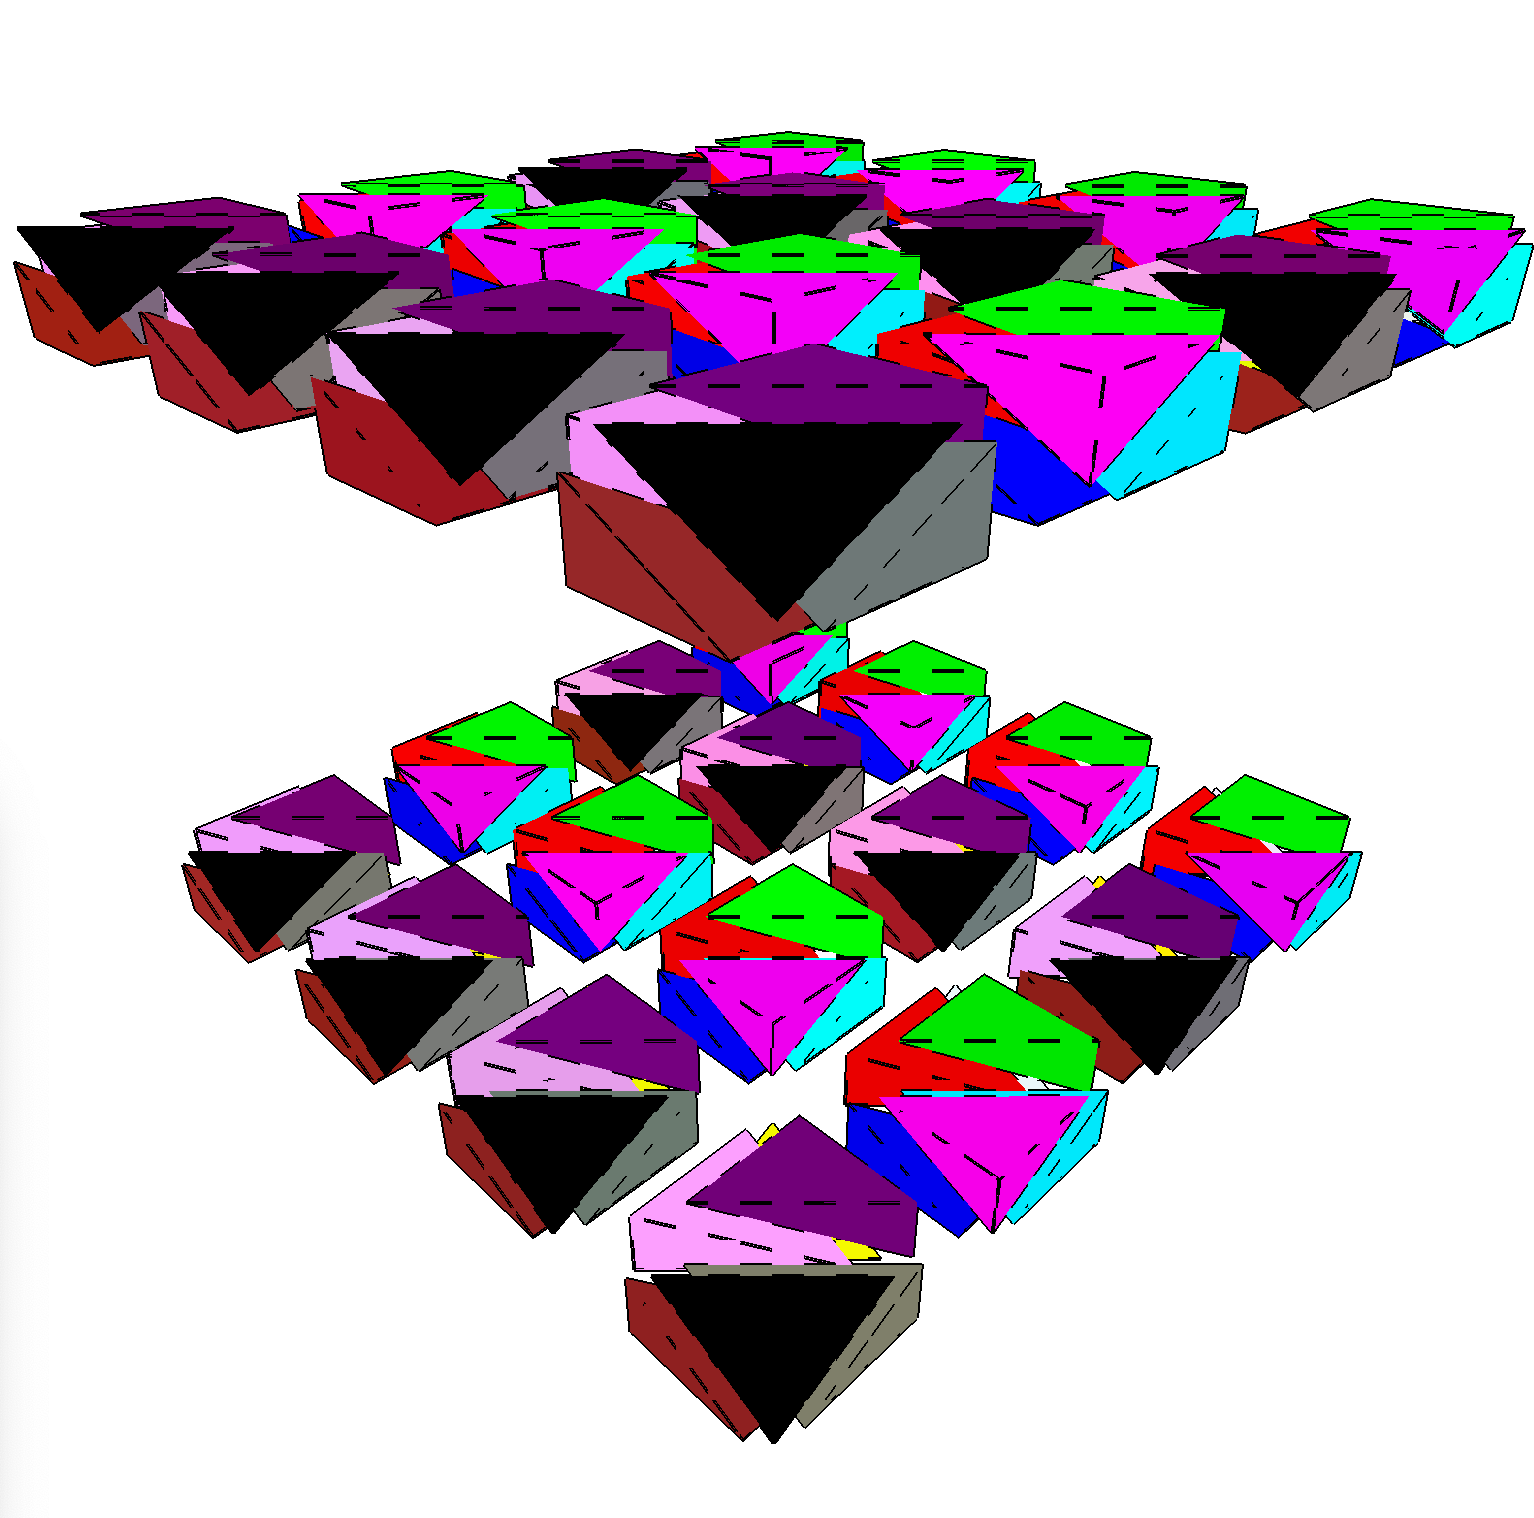
\includegraphics[eight=0.33\linewidth,width=0.33\linewidth]{chapter-03/figs/extrude05.png}\hfill
   \caption{Exploded simplicial grids of dimensions 1 (lines), 2 (surfaces), and 3 (solids). The simplicial 2-complex is generated by \emph{simplexfacets()} from the 3-complex \emph{extrudecomplex(simplex2D)}, with \emph{simplex2D} in turn starting from \emph{model1D}, i.e., from the expression generating the simplicial 1-complex \inlinegraphics{chapter-03/figs/complex1D.png}. }
   \label{fig:3:extrude2}
\end{figure}



\subsection{Cubical complex and grid}\label{sect:3-2-2}


We introduce now the definition and use of multidimensional \emph{grids} of \emph{cuboidal}, and the more general \emph{Cartesian product} of cellular complexes. Such operators, depending on the dimension of their input, may generate either \emph{full-dimensional} (i.e. solid) output complexes, or \emph{lower-dimensional} complexes of dimension $d$ embedded in Euclidean $n$-space, with $d\leq n$.  

\subsubsection*{Regular grid}


Regular cubical grids of appear on graph paper and may be used in finite element analysis, finite volume methods, finite difference methods, and in general for discretization of parameter spaces. 

\begin{definition}[Regular grid] A regular grid is a tessellation of n-dimensional Euclidean space by congruent parallelotopes (e.g. bricks). Its opposite is irregular grid.
\end{definition}

E.g., just think to a mesh of 3D cubes in three-dimensional space for the first case, and to the (non-manifold) framework of boundary polygons of such cubic cells for the second case.
In particular,  both $n$-dimensional \emph{solid grids} of (hyper)-cuboidal cells and their  $d$-dimensional \emph{skeletons} ($0\leq d\leq n$), embedded in $\E^n$, are generated by assembling the cells produced by a product of $n$ either 0D or 1D cellular complexes, that in such lowest dimensions coincide with \emph{simplicial complexes}. 







\subsection{Polyhedral complex}\label{sect:3-2-3}


\subsection{Topological product}
\label{subsec:2:style}

In this section, we discuss a solid modeling operation highly useful to generate 3D solids from 2D surfaces, as well as 2-complexes from 1-complexes, and to produce their skeletons taking advantage of one or more 0-complexes.

\begin{definition}[Topological product]
A product space is the \emph{Cartesian product} of a family of topological spaces equipped with a natural topology.
\end{definition}

The natural topology on a subset of a topological space, in our case $\E^d$, is the relative topology (or subspace topology).
The product of two cell complexes can be made into a cell complex as we show in the following. 

\begin{definition}[Product of cell complexes]
If $X$ and $Y$ are  $m$- and $n$-complexes in $\E^m$ and $\E^n$, respectively,  $X \times Y \subset \E^{m+n}$ is a cell complex in which each cell is a product of a cell in $X$ and a cell in $Y$, endowed with the relative topology in $\E^{m+n}$.
\end{definition}

\subsection{Cell complex product}
\label{subsec:6:cell-product}

\begin{definition}[larprod]
The |larprod| function takes as input a pair of |Lar| models and returns the model of their \emph{Cartesian product}. Since the |Lar| type is a pair (\emph{geometry, topology}), the 
output of |larprod( lar1, lar2 )| is the \emph{topological product} of the input |Lar| values.
\end{definition}



\section{Chain complex}\label{sect:3-3}

\subsection{Linear chain spaces}\label{sect:3-3-1}


\subsection{Linear chain operators}\label{sect:3-3-2}


\subsubsection*{Matrix-Vector Products as Linear Combinations}
Left-multiply a matrix $\T{A}$ by a \emph{row vector} $\v{x}$, i.e. $\v{x}\T{A}$, is a linear combination of \T{A} rows with $\v{x}$ elements as scalars, and produces a row vector. 
Analogously, right-multiply a matrix $\T{A}$ by a \emph{column vector} $\v{x}$, i.e. $\T{A}\v{x}$, is a linear combination of \T{A} columns, and produces a column vector. 
\end{definition}

In this book we often use a pair of characters from $\{$|V|, |E|, |F|$\}$, for instance |EF|, to denote the mapping |F|${}\to{}$|E| from 2-chains in |F| to 1-chains in |E| (see Section~\ref{}).



\begin{coding}[Construction of operator matrix] [$\partial_2$].
With some abuse of language (removed after Section~\ref{sec:2:chaincomplexes}), we build the sparse matrix of |EF $\equiv$ ∂₂: F $\to$ E|. 
\lstinputlisting[language=JuliaLocal,style=julia,mathescape=false]{/Users/paoluzzi/Documents/dev/PLASM/SPRINGER/BOOK/chapter-06/code/006.jl}
It may be interesting to make some notation about this matrix. Remember that, by right multiplication, any mapping matrix sends the space of columns (2-chains: triangles here) to the space of rows (1-chains: edges here). With any simplicial complex we have two 1s on each row and three 1s on each column. They characterize the two faces incident on the edge, and the three edges incident on the face, respectively.
\end{coding}


\begin{coding}[How to use the linear operators.]
A boundary operator, which is a linear map, sends every vector in domain space (the span of the matrix columns) to its image vector in target space (the span of the matrix rows). 
\lstinputlisting[language=JuliaLocal,style=julia,mathescape=false]{/Users/paoluzzi/Documents/dev/PLASM/SPRINGER/BOOK/chapter-06/code/007.jl}
In particular, the matrix of a linear operator---coordinate representation of it with respect to the chosen bases---send the coordinate representation of a domain vector to its image in target space. Both are binary vectors, as will be clear after Section~\ref{sec:2:chaincomplexes}. E.g.,  |face[4]| has boundary edges 3, 4, and 12 (look for |1|s positions in row 5 above).
\end{coding}


\section{Cochain integration (surface, volume, inertia)}\label{sect:3-4}






\begin{coding}[Volume of a cube from boundary triangles].
The variable |obj| first contains the memory pointer to an object of type |Hpc|, then to an object of type |Lar|. Here, |obj.C| gives the dictionary |C| of its cell complex, where |C[:FV]| denotes the array of boundary faces (triangles).
\begin{lstlisting}[language=JuliaLocal, style=julia, mathescape = true]
julia> obj = SIMPLEX(3)
Hpc(MatrixNd(4), Geometry([[0.0, 0.0, 0.0], [1.0, 0.0, 0.0], [0.0, 1.0, 0.0], [0.0, 0.0, 1.0]], hulls=[[1, 2, 3, 4]]))

julia> obj = LAR(SIMPLEX(3))
Lar(3, 3, 4, [0.0 1.0 0.0 0.0; 1.0 0.0 0.0 0.0; 0.0 0.0 0.0 1.0], Dict{Symbol, AbstractArray}(:CV => [[1, 2, 3, 4]], :FV => [[1, 2, 3], [2, 3, 4], [1, 3, 4], [1, 2, 4]], :EV => [[2, 3], [1, 3], [1, 2], [3, 4], [2, 4], [1, 4]]))

FV = obj.C[:FV]  #=
4-element Vector{Vector{Int64}}:
 [1, 2, 3]
 [1, 2, 4]
 [1, 3, 4]
 [2, 3, 4]   =#
P = (obj.V, FV); VOLUME(P)  #=
0.16666666666666666   =#
volume(P) * 6   #=
1.0   =#
\end{lstlisting}
\end{coding}



%%%%%%%%%%%%%%%%%%%%%part.tex%%%%%%%%%%%%%%%%%%%%%%%%%%%%%%%%%%
% 
% sample part title
%
% Use this file as a template for your own input.
%
%%%%%%%%%%%%%%%%%%%%%%%% Springer %%%%%%%%%%%%%%%%%%%%%%%%%%

\begin{partbacktext}
\part{Dimension-independent Modeling}


% !TEX TS-program = xelatex

\chapter{Geometric models}
\label{chapt:4}

Julia |Plasm| is the best choice to write symbolic geometric models for Building Information Modeling (BIM) and Computer-Aided Design (CAD).  Geometric models specify the physical appearance of Architecture, Engineering, and Construction products at any scale, from structural and envelope components to whole buildings and built environments, and are used for design, tender, contract, and collaboration. We ported the  functional language |Plasm| to Julia for better supporting design, model generation, and visualization of geometric objects.
In this chapter we introduce the great expressive power of |Plasm| geometric types and parametric functions, as well the simple methods used to build parametric assemblies, where objects itself can be used as actual parameters. We show also that |Plasm| offers a  general mechanism (Julia dictionaries) to export models characterized by colors, textures, materials, and so on. |Plasm| can be even embedded in the |Juπpiter| platform in order to document the design choices step-by-step in digital notebooks.

\section{Plasm geometric types}\label{sect:4-1}

Even if Julia does not pretend the user specifies the type of data objects, which are inferred at compile time, it may always be useful to annotate with their type the parameters and the returned value from function applications in order to get faster codes from the Julia compiler. The best reason concerns program documentation, making it easier to understand the Julia's sources.

Let's remember that |Plasm| derives from three founts: (1) the |PLaSM| classic set up on |FL| functional combinators; (2) the porting to Python (object-oriented language), and finally (3) the embedding into Julia (functional and multi-paradigm), after several years of algebraic research finalized to understand the role of topology in elaborating digital  geometric models. 

This development defined different data types and user structures, which the current version of the language proudly unifies by scheduling them to different roles and uses.
 

\begin{enumerate}
\item 
The Hierarchical Polyhedral Complex, now denoted in Julia |Plasm| as the |Hpc| datatype, was characterized by models defined as aggregation of multidimensional convex cells, described only by their vertices and by multidimensional affine matrices.

\item 
Our research about algebraic topology of geometric design directed us to design the Linear Algebraic Representation, currently the |Lar| datatype, used to work with chain complexes, and able to  fully specify the geometry and topology of the \emph{solid objects} under consideration, even non-manifold.

\item 
Finally, a third Julia’s user-defined |struct|, named |Geo| for Geometry, is being used as container of huge datasets for |Plasm|-coded generation of |BIM| objects and 3D point clouds from surveys.  
\end{enumerate}


\subsection*{Hpc Type}\label{sect:4-1-1}

This recursive type is mainly used for geometric object definition, including the hierarchical values generated by the |STRUCT| function, and interactive graphics visualization on the display device.

An object of |Hpc| type has three fields: a multidimensional matrix |T::MatrixNd|; a vector |childs| (i.e., children) either of elements |Hpc| or of elements |Geometry|, and a |Properties| field of dictionary type, i.e., |Dict{Any, Any}|.

The |mutable struct Hpc| is a typical recursive data structure to represent dynamically a data object of tree type, where the | children | nodes of a node may be in any number since stored into a Julia’s |Vector|.

\begin{lstlisting}[language=JuliaLocal, style=julia, mathescape = true] 
mutable struct Hpc
T::MatrixNd
childs::Union{Vector{Hpc}, Vector{Geometry}}
properties::Dict{Any, Any}
# constructor
   function Hpc(T::MatrixNd=MatrixNd(0), childs:: Union{Vector{Hpc}, Vector{Geometry}}=[], properties=Dict())
      self = new()
      self.childs = childs
      self.properties = properties
      if length(childs) ) 0
         Tdim = maximum([dim(child) for child in childs]) + 1
         self.T = embed(T, Tdim)
      else
         self.T = T
      end
      return self
   end
end
\end{lstlisting}



\subsection*{Lar Type}\label{sect:4-1-2}

The |mutable struct Lar| is used to represent synthetically a generic cellular or chain complex, together with some of its properties. Given |obj::Lar|, it represents with |obj.d|, |obj.m|, |obj.n|, |obj.V|, and |obj.C|, respectively, the intrinsic dimension (1 for curves, 2 for surfaces, 3 for solids), the number of its coordinates, the number of vertices, and a dictionary of of chain bases or chain operators, stored when already available throughout a computation.

\begin{lstlisting}[language=JuliaLocal, style=julia, mathescape = true] 
mutable struct Lar
   d::Int # intrinsic dimension
   m::Int # embedding dimension (rows of V)
   n::Int # number of vertices  (columns of V)
   V::Matrix{Float64} # object geometry
   C::Dict{Symbol, AbstractArray} # object topology (C for cells) 
   # inner constructors
   Lar() = new( -1, 0, 0, Matrix{Float64}(undef,0,0), Dict{Symbol, AbstractArray}() )
   Lar(m::Int,n::Int) = new( m,m,n, Matrix(undef,m,n), Dict{Symbol,AbstractArray}() )
   Lar(d::Int,m::Int,n::Int) = new( d,m,n, Matrix(undef,m,n), Dict{Symbol,AbstractArray}() ) 
   Lar(V::Matrix) = begin m, n = size(V); new( m,m,n, V, Dict{Symbol,AbstractArray}() ) end
   Lar(V::Matrix,C::Dict) = begin m,n = size(V); new( m,m,n, V, C )  end
   Lar(d::Int,V::Matrix,C::Dict) = begin m,n = size(V); new( d,m,n, V, C )  end
   Lar(d,m,n, V,C) = new( d,m,n, V,C )
end
\end{lstlisting}



\subsection*{Geo type}\label{sect:4-1-3}

A |mutable struct Geometry| is used as a container for single whole geometric objects, allowing to store the various dimensional cellular subcomplexes that partition the geometric value. Conversely, any hierarchical assembly is stored in |Plasm| within a mixture of |Hpc| and |Geometry| nodes. The |Geometry| data structure contains arrays of integers, denoting the ordered bases of the topological chains of different dimensions that decompose the represented geometric value. It also contains a numeric |db| (data base), implemented as a Julia dictionary with key the (suitably rounded) coordinate vector sof vertex |point| and with value the corresponding integer index.

\begin{lstlisting}[language=JuliaLocal, style=julia, mathescape = true] 
mutable struct Geometry
   db::Dict{Vector{Float64}, Int}
   points::Vector{Vector{Float64}}
   edges::Vector{Vector{Int}}
   faces::Vector{Vector{Int}}
   hulls::Vector{Vector{Int}}
   # constructor
   function Geometry()
   self = new(
      Dict{Vector{Float64}, Int}(),
      Vector{Vector{Float64}}(),
      Vector{Vector{Int}}(),
      Vector{Vector{Int}}(),
      Vector{Vector{Int}}(),
   )
   return self
   end
end
\end{lstlisting}


\subsection*{Topological types}\label{sect:4-1-4}

Some abstract types are defined in |Plasm| in order to characterize and document the type of variables and/or parameters within complicated definitions and function codes. They are mainly used within the structures of |Lar| type, to document the topology, and are defined as global |const| symbols.

\begin{lstlisting}[language=JuliaLocal, style=julia, mathescape = true] 
const Points = Matrix{number}
const Cells = Vector{Vector{Int}}
const Cell = SparseVector{Int8, Int}
const Chain = SparseVector{Int8,Int}
const ChainOp = SparseMatrixCSC{Int8,Int}
const ChainComplex = Vector{ChainOp}
\end{lstlisting}

The |Cells| type stores the cellular bases and some subsets of cells as |Vector| of |Vector| of integers. The |Cell| type is utilized to memorize a single cell's (sparse)  representation. The |Chain| type item equals the cell type, and is used only for documentation aims. The |ChainOp| type allows the storage of the topological operators, including boundary and coboundary, and other higher degree operators, e.g., |FV|. The |ChainComplex| type is employed as the multidimensional |Vector| store of chain complexes, by now only in 2D and 3D, with two and three |ChainOp| sparse matrices, respectively.

\begin{coding}[3-cube topology is a ChainOp object]\
The expression |cube.C[:FV]| returns a dictionary value of type |Cells|, which contains the basis of our cubic cellular complex.  |KFV| is of type |ChainOp|:

\begin{lstlisting}[language=JuliaLocal, style=julia, mathescape = true] 
cube = LAR(CUBE(3))			#=
Lar(3, 3, 8, [3.0 0.0 … 3.0 0.0; 3.0 3.0 … 3.0 3.0; 0.0 0.0 … 3.0 3.0], Dict{Symbol, AbstractArray}(:CV =) [[1, 2, 3, 4, 5, 6, 7, 8]], :FV =) [[1, 2, 3, 4], [3, 4, 5, 6], [1, 3, 5, 7], [2, 4, 6, 8], [1, 2, 7, 8], [5, 6, 7, 8]], :EV =) [[3, 4], [2, 4], [1, 2], [1, 3], [5, 6], [4, 6], [3, 5], [5, 7], [1, 7], [6, 8], [2, 8], [7, 8]])) =#

FV = cube.C[:FV]			#=
6-element Vector{Vector{Int64}}:
 [1, 2, 3, 4]
 [3, 4, 5, 6]
 [1, 3, 5, 7]
 [2, 4, 6, 8]
 [1, 2, 7, 8]
 [5, 6, 7, 8]			=#

KFV = lar2cop(FV::Cells)::ChainOp		#=
6×8 SparseArrays.SparseMatrixCSC{Int8, Int64} with 24 stored entries:
 1  1  1  1  ⋅  ⋅  ⋅  ⋅
 ⋅  ⋅  1  1  1  1  ⋅  ⋅
 1  ⋅  1  ⋅  1  ⋅  1  ⋅
 ⋅  1  ⋅  1  ⋅  1  ⋅  1
 1  1  ⋅  ⋅  ⋅  ⋅  1  1
 ⋅  ⋅  ⋅  ⋅  1  1  1  1			=#
\end{lstlisting}
Of course, |(typeof(FV)==Cells) && (typeof(KFV)==ChainOp) # =) true|, 
since |lar2cop| : Cells $\to$ |ChainOp|.
\end{coding}

\begin{remark}[About sparsity]
While in this small case, the |KFV| matrix is not very sparse, the sparsity overgrows as the cellular complex proliferates, since the non-zero elements grow linearly with the number of cells. In contrast, the zero elements grow quadratically (with the matrix dimension).
\end{remark}
\begin{remark}[Global view of incidencies]
See, by inspection of |KFV|, that each face is incident to 4 cube vertices and each vertex is incident to 3 faces.
\end{remark}


\section{Plasm parametric primitives}\label{sect:4-2}

In this section, we introduce and exemplify several features of |Plasm| working with geometric objects. The |Plasm| package is quite different from most geometric and graphics |API|s since it is based on |FL|-style combinators.


\subsection{Geometric Transformations}\label{sect:4-2-1}

The user interface to affine coordinate transformation of geometric objects is given through standard Julia functions and matrices. Internally, |Plasm| implements such mapping of local coordinates using its own multidimensional matrix type, called |MatrixNd|, and the use of the field |T::MatrixNd| within the recursive datatype |Hpc|.

\begin{definition}[Geometric transformation]
A \emph{geometric transformation} is a bijective function, i.e., a one-to-one (injective) and onto (surjective) mapping $\mathbb{E}^d \to \mathbb{E}^d$. 
\end{definition}

By definition, geometric transformations of plane or space are invertible, and hence represented by invertible square matrices. We will see that \emph{rotation}, \emph{scaling}, and \emph{shearing} are linear transformations; \emph{translation} is affine. 


\subsubsection*{Homogeneous Coordinates}

In computer graphics the \emph{homogeneous coordinates} are often used instead of Cartesian coordinates. In the homogeneous plane or space, lines are mapped to lines, but parallel lines are not conserved parallel. The main reason for this change is the ability to treat affine maps (translation) as linear, and combine smoothly with linear maps (rotation, scaling, etc.)

In homogeneous coordinates the Euclidean plane $\mathbb{E}^2 \,\backslash\, \{\v{0}\}$ is considered in bijective correspondence with the bundle of lines in $\mathbb{E}^3 \,\backslash\, \mathbb{E}^2$ (a model for the projective plane) so that each point $(x,y)\in\E^2$ corresponds to a line $\lambda(W, X, Y)$ such that $(x, y) \equiv \frac{W}{W}, \frac{X}{W}, \frac{Y}{W}) = (1, x, y)$. Same for each $\E^d$, $d \geq 2$. After the division, homogeneous coordinates are said \emph{normalized}.

\begin{figure}[htbp] %  figure placement: here, top, bottom, or page
   \sidecaption[t]
   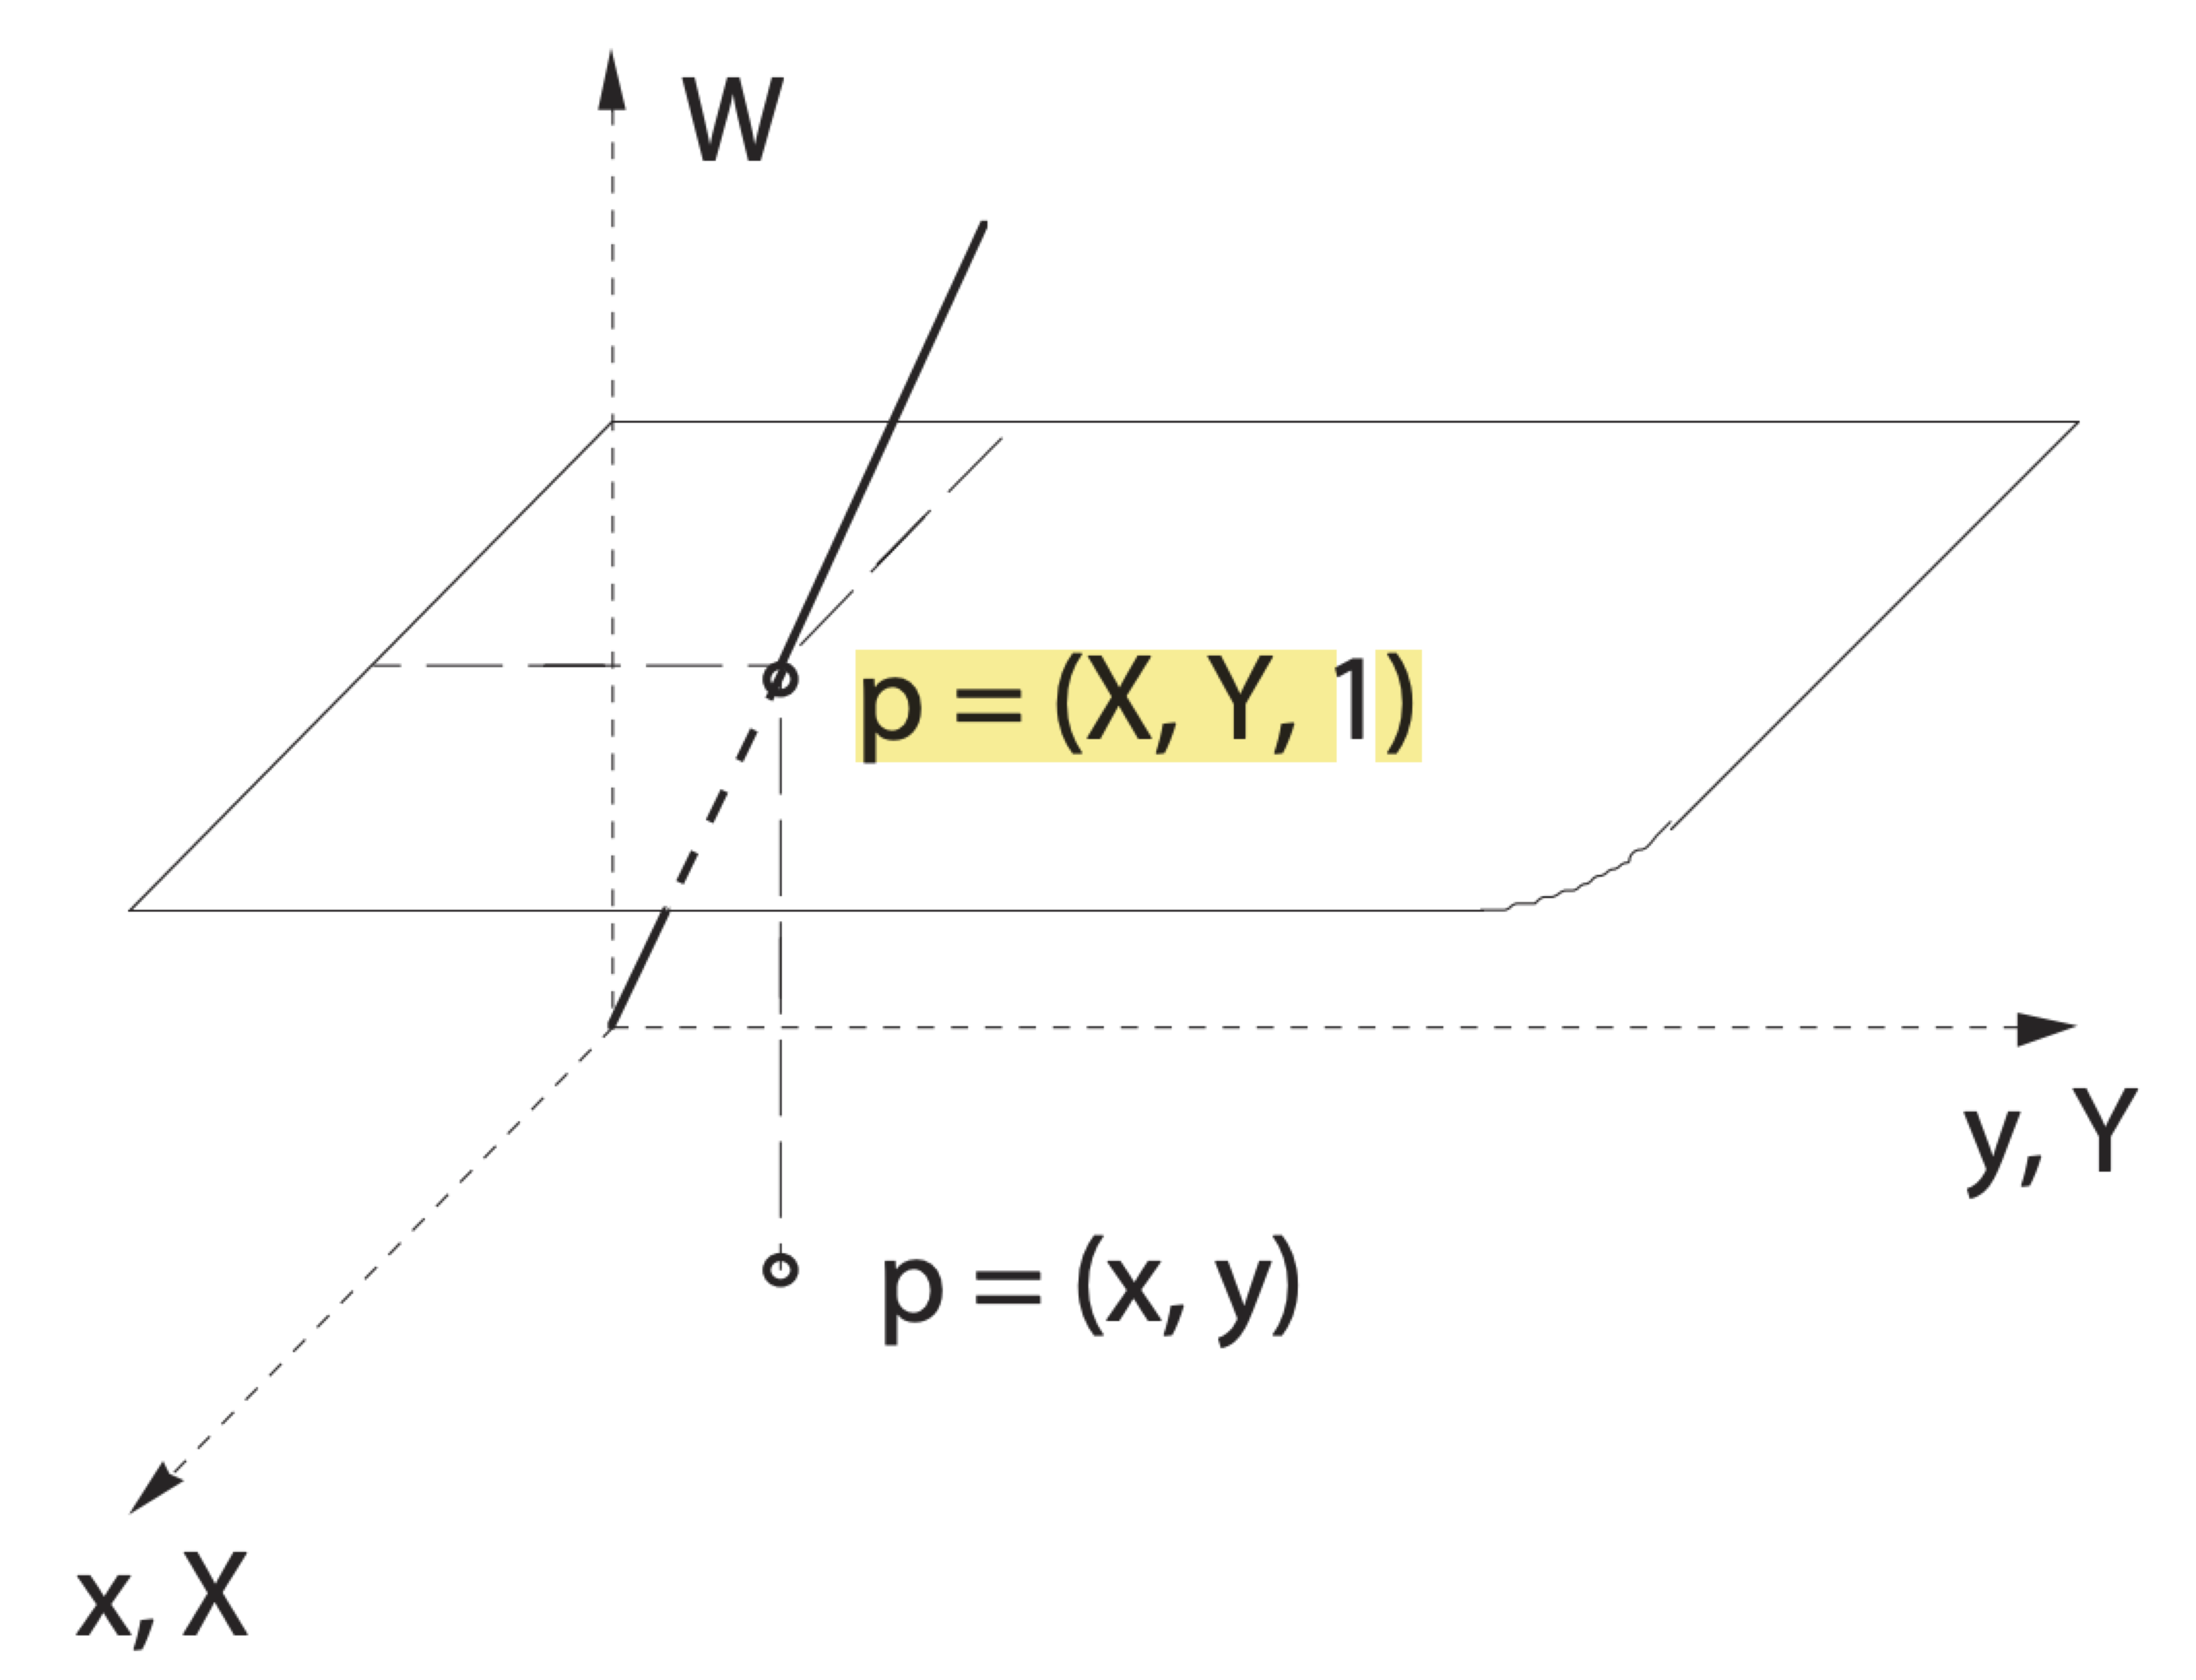
\includegraphics[width=2in]{chapter-04/figs/homog-2d} 
   \caption{The homogeneous plane is a model of a projective plane, where all finite points have a homogeneous coordinate equal to one, and the points at infinity have it equal to zero. All the points at infinity form the line at infinity, and all the lines at infinity form the plane at infinity.}
   \label{fig:example}
\end{figure}

In |Plasm|, by design choice to make the multidimensional approach to geometric design more accessible, the added homogeneous coordinate is the first, not the last, as we may see in many computer graphics books.

Even more, for the sake of clarity, we can use the |HOMO| operator to transform a $d\times d$ matrix in a $(d+1)\times(d+1)$ matrix, i.e., a $3\times 3$ on the 2D plane and $4\times 4$ on 3D space. The type of returned matrix is |MatrixNd|, which is used for dimension-independent programming.

Homogeneous coordinates allow to combine linearly all transformations, using products of their matrices in homogeneous coordinates. In the remainder of this section we describe the geometric effect of each transformation and the structure of the corresponding matrices. 

\begin{remark}The reader should note that our maps or transformations are invertible functions of a space into itself (automorphisms), represented (even translation, as we will see) by square matrices, i.e. are \emph{rank 2} tensors. Since they are also |Plasm| functions, can be \emph{applied} to geometric objects; as matrices, they multiply the object coordinates.
\end{remark}




\subsection*{2D rotation}\label{sect:4-2-1}

In a \emph{planar rotation} all points of the 2D plane move along an arc of circle, with same angle at center, while the center is the only fixed point. In  a \emph{space rotation} there is a straight line of fixed points (the axis) passing for the origin. All the other 3D points describe a circle arc with the same angle along the plane (orthogonal to rotation axis) which they belong to. 

Let us show (see Figure~\ref{fig:rotmatrix}) how unit vectors $\v{e}_1 = \vet{1 \\ 0}$ and $\v{e}_2 = \vet{0 \\ 1}$, columns of the matrix $\mat{\v{e}_1 & \v{e}_2 } $ are transformed by the (yet unknown) $\T{R}(\alpha)$ rotation matrix into the columns of the matrix at right-hand side:
\[
\mat{\cos\alpha & -\sin\alpha\\ \sin\alpha & \cos\alpha}
=
\T{R}(\alpha)\,\mat{\v{e}_1 & \v{e}_2 }. 
\quad
\mbox{Hence we have:}
\quad
\T{R}(\alpha) = \mat{\cos\alpha & -\sin\alpha\\ \sin\alpha & \cos\alpha}
\]


There is only one class of planar rotations, parameterized by $\alpha$, the \emph{rotation angle} about the origin. Conversely, we will see three classes of elementary space rotations, parameterized by $\alpha_x, \alpha_y, \alpha_z$, the rotation angles about each coordinate axis.


\begin{coding}[Plasm notation for rotation]
The plane rotation function in |Plasm| is: |R([1,2])($\alpha$)| because its effect is to change the first and second coordinates of the 2D model it is applied to. They are applied to a planar geometric object of |Hpc| type, by using the |STRUCT| operator (see Section~\ref{}) that contains |Hpc| values and transformation tensors:
\begin{lstlisting}[language=JuliaLocal, style=julia, mathescape=true]
SQUARE(d) = CUBOID([d,d])		#=
SQUARE (generic function with 1 method)		=#

obj = R(1,2)(π/4)(SQUARE(1))		#=
Hpc(MatrixNd([[1.0, 0.0, 0.0], [0.0, 0.7071067811865476, -0.7071067811865475], [0.0, 0.7071067811865475, 0.7071067811865476]]), Hpc(MatrixNd(3), Hpc(MatrixNd(3), Geometry([[0.0, 0.0], [1.0, 0.0], [1.0, 1.0], [0.0, 1.0]], hulls=[[1, 2, 3, 4]])))) =#

VIEW(obj)
\end{lstlisting}
\end{coding}

\begin{remark}
|CUBOID(shape)::Hpc| is the generator of multidimensional hyper-par\-allelo\-pipeds, depending on length and content of |shape| vector. 

|CUBOID([1,1])| is the unit square;  |CUBOID([1,2,3])| is the parallelopiped of sides 1, 2, and 3; 
|CUBOID([1,1,1,1])| is the 4D unit hypercube.
\end{remark}


\subsection*{Elementary rotations}

The multidimensional |Plasm| language has the following definition of elementary rotation, that allows to rotate a $r$-model ($r\leq d$) in any dimension $d\geq 2$.

\begin{definition}[Elementary rotation]
The reader should note that the \emph{elementary} rotation is defined in any dimension $d$  such that only $2$ coordinates are changed by the rotation.
\end{definition}

\begin{remark}
It is easy to see that in any dimension $d$ there are |binomial$(d,2)$| elementary rotations, how many are the ways to choose $2$ coordinates over $d$. Hence we have $1$ for $d=2$, 3 for $d=3$, 6 for $d=3$, and so on.
\end{remark}


Assume that the rotation axes are $\v{e}_1, \v{e}_2, \v{e}_3$, with rotation angles $\alpha, \beta, \gamma$ respectively. The corresponding elementary matrices, derivable as before by change of coordinates, are:
\begin{equation}\footnotesize
\T{R}_x(\alpha) = \mat{1 & 0 & 0 \\ 0 & \cos\alpha\ &  -\sin\alpha\\ 0 & \sin\alpha & \cos\alpha},\ 
\T{R}_y(\beta) = \mat{\cos\beta & 0 & \sin\beta\\ 0 & 1 & 0 \\ -\sin\beta\  &  0 & \cos\beta},\ 
\T{R}_z(\gamma) = \mat{\cos\gamma & -\sin\gamma & 0\\ \sin\gamma & \cos\gamma & 0\\ 0 & 0  &1}
\end{equation}

In |Plasm| the elementary rotations are represented, respectively, by the tensors: |R([2,3])($\alpha$)|, |R([1,3])($\beta$)|, and |R([1,2])($\gamma$)|. 
\begin{coding}[Elementary rotation] We use an interesting 3D polyhedron, called permutahedron, to show the application of the tensor |R([1,2])(pi/2)| to it:
\begin{lstlisting}[language=JuliaLocal, style=julia, mathescape=true]
obj = R([1,2])(pi/2)( PERMUTAHEDRON(3) );
VIEW( obj )
\end{lstlisting}
\end{coding}

\begin{remark}[Reduction of visual noice]
Just note that in all |Plasm| geometric operators, the constraint of using functions as unary has been relaxed, in order to make possible to write, e.g., |obj = R(1,2)(pi/2)(obj)| instead than |obj = R([1,2])(pi/2)(obj)|. In the remainder we use always this new style.
\end{remark}


\begin{coding}[Permutahedron] The reader might be curious to see how such important and beautiful polyhedron~\cite{wiki:pao:100} whose vertex coordinates are the permutations of the first $d$ natural numbers. Iy is generated in |Plasm|:
\begin{lstlisting}[language=JuliaLocal, style=julia, mathescape=true]
function PERMUTAHEDRON(d)
	vertices = ToFloat64(PERMUTATIONS(collect(1:d+1)))
	center = MEANPOINT(vertices)
	cells = [collect(1:length(vertices))]
	object = MKPOL(vertices, cells, [[1]])
	object = T(INTSTO(d))(-center)(object)
	for i in 1:d
		object = R(i,d+1)(pi/4)(object)
	end
	object = PROJECT(1)(object)
	return object
end
\end{lstlisting}
The |Plasm| function |INTSTO($d$)| (integers to $d$) is used to generate the sequence |[1,2,$\ldots$,d]|, extremes included. The other functions are easy to understand.
\end{coding}




\subsection*{General rotation in 3D}

A rotation of 3D space has a fixed line of points (the rotation axis) passing through the origin. We may compute the corresponding matrix as a function of a direction vector for the axis and a real value for the rotation angle. For this purpose we can compone three linear transformations by multiplication of their matrices.  Therefore we have:

\begin{definition}[General 3D rotation with axis $d$ and angle $\alpha$]
Clearly, the ordering of transformations is from right to left:
\[
\T{R}(\v{d},\alpha) = \T{Q}^{-1}(\v{d})\, \T{R}_z(\alpha)\, \T{Q}(\v{d})
\]
First, a space rotation that brings the vector $d$ on a coordinate axis, say $\v{e}_3$; second, a space rotation $\T{R}_z(\alpha)$ about the $z$-axis; third, the inverse of the first transformation, so to bring the rotation axis in its original direction.
\end{definition}

$\T{Q}(\v{d})$ must transform the unit vector $\v{d}$ to the $\v{e}_3$ unit vector. So, we may compute the coordinate transformation that brings three orthonormal vectors $(\v{u}_1, \v{u}_2, \v{u}_3)$ to become the standard basis $(\v{e}_1, \v{e}_2, \v{e}_3)$. We can choose the triple:
\begin{eqnarray}
\v{u}_3 &=& \v{d}/\,\|\v{d}\|,\nonumber\\
\v{u}_2 &=& (\v{u}_3 \times \v{e}_3)/\,\|\v{u}_3 \times \v{e}_3\|,\\
\v{u}_1 &=& \v{u}_2 \times \v{u}_3,\nonumber
\end{eqnarray}
to write the transformation of coordinates:
\[
(\v{e}_1, \v{e}_2, \v{e}_3) = \T{Q}(\v{d})\, (\v{u}_1, \v{u}_2, \v{u}_3)
\]
so that we have:
\[
\T{Q}(\v{d}) = (\v{u}_1, \v{u}_2, \v{u}_3)^{-1}
\]
But $\T{Q}(\v{d})$ maps orthonormal vectors to orthonormal vectors, hence it is a normal
transformation, so its inverse is equal to its transpose. So, we can write:
\begin{equation}
\T{R}(\v{d},\alpha) = \T{Q}^{t}(\v{d})\, \T{R}_z(\alpha)\, \T{Q}(\v{d}).
\end{equation}


\begin{coding}[3D General Rotation matrix]
Let’s use a test-driven programming style, with parameter values easy to test
Rotate of 45 degrees about the diagonal axis the unit cube with a vertex on the origin, i.e. the model generated by the |CUBE(1)| expression in |Plasm|. 
We may follow this procedure using a functional approach:

\begin{lstlisting}[language=JuliaLocal, style=julia, mathescape=true]
using Plasm, LinearAlgebra
d = [1,1,1];
u₃ = normalize(d);
u₂ = normalize(u₃ × [0,0,1]);
u₁ = u₂ × u₃;
\end{lstlisting}
and write the following matrix for the transformation of coordinates that maps the $\v{e}_3$ axis to the direction of the |d| vector. 
\begin{lstlisting}[language=JuliaLocal, style=julia, mathescape=true]
Q(d) = [u₁ u₂ u₃]'
\end{lstlisting}
The single quote stands for the Julia |transpose| of a matrix.
\end{coding}


\begin{figure}[htbp] %  figure placement: here, top, bottom, or page
\begin{minipage}[c]{0.35\textwidth}
   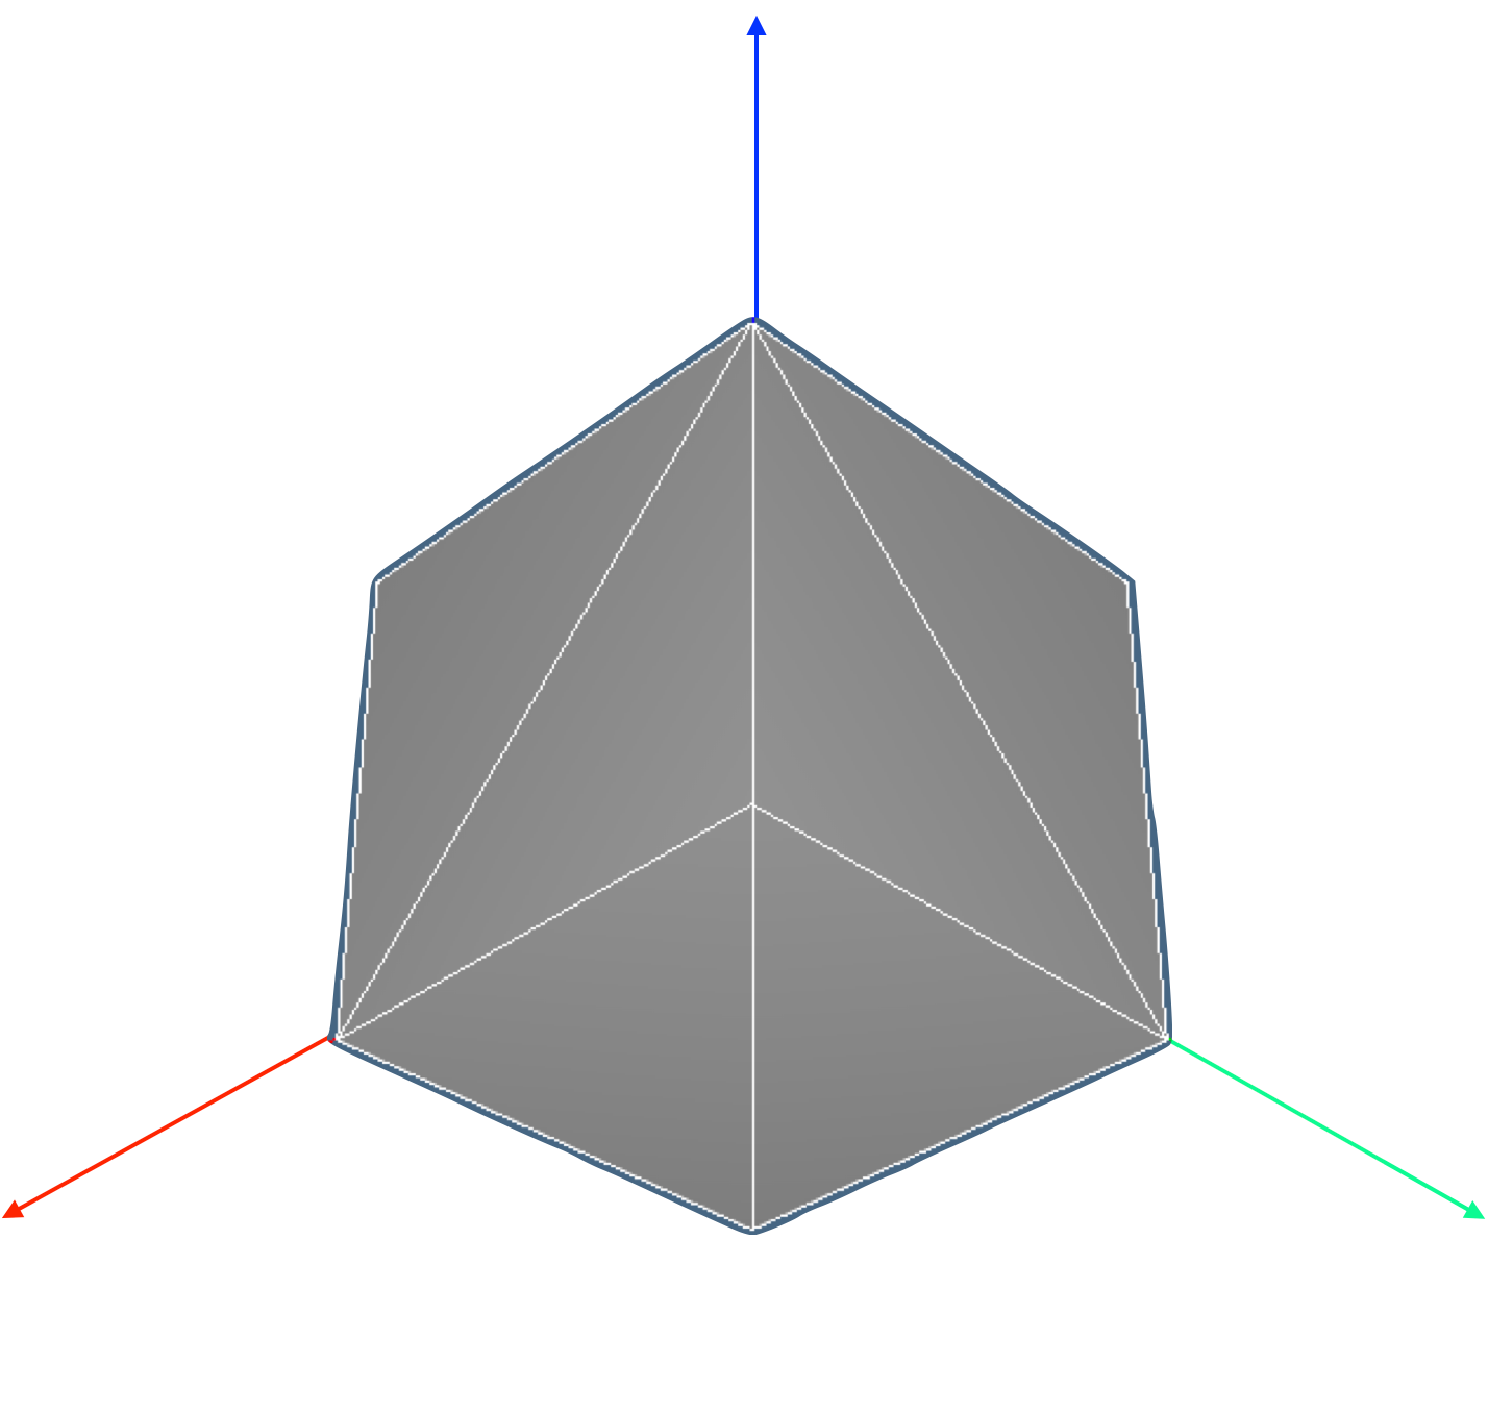
\includegraphics[width=2in]{chapter-04/figs/GRcube} 
\end{minipage}
\hfill
\begin{minipage}[c]{0.55\textwidth}
\begin{lstlisting}[language=JuliaLocal, style=julia, mathescape=true]
rotated = GR([1,1,1],π/3)(CUBE(1))
VIEW(rotated)
\end{lstlisting}
\caption{General rotation (GR) of angle $\pi/3$ about axis [1,1,1]. }
\end{minipage}
\end{figure}


\begin{coding}[General 3D rotation tensor]
In what follows, |MAT| transforms a Julia |Matrix| into a |Plasm| tensor applicable to |Hpc| values. 
The |HOMO| function apply to  a square matrix, adding new unitary first row and column, for homogeneous coordinates (see Section~\ref{}).  
\begin{lstlisting}[language=JuliaLocal, style=julia, mathescape=true]
GR(d,α) = MAT(HOMO(Q(d)')) ∘ R(1,2)(α) ∘ MAT(HOMO(Q(d)))
\end{lstlisting}
The |GR| (general rotation) is a |Plasm| tensor depending on the axis |d| and the angle |$\alpha$|. 
Our geometric model is therefore rotated and viewed as follows.
\end{coding}



\subsection*{Scaling}\label{sect:4-2-2}

In a scaling transformation, all points are moved along the line passing for the origin they belong to.  The scaling is said \emph{elementary} when only one of the coordinates changes. There are two scaling parameters $s_x, s_y$ in 2D geometry and three scaling parameters $s_x, s_y, s_z$ in 3D, to be used in scalar products by the point coordinates.
The transformation can be a \emph{dilatation} of space when scaling parameters are greter than one, or a \emph{contraction} of space when scaling parameters are lesser than one.
\[
S(s_x,s_y,s_z) = \mat{s_x & 0 & 0\\ 0 & s_y & 0\\ 0 & 0 & s_z},\ 
S_x = \mat{s_x & 0 & 0\\ 0 & 1 & 0\\ 0 & 0 & 1},\ 
S_y = \mat{1 & 0 & 0\\ 0 & s_y & 0\\ 0 & 0 & 1},\ 
S_z = \mat{1 & 0 & 0\\ 0 & 1 & 0\\ 0 & 0 & s_z} 
\]
The scaling matrices are diagonal.
The origin remains fixed. In fact: \[S\,\vet{0 &0 & 0}^t = \vet{0 & 0 & 0}^t.\] 
Hence, a scaling transformation is linear. It is easy to see that  scale transformations are multiplicative, commutative, and associative because the matrix is diagonal:
\[
\T{S}(s_x, s_y, s_z) = \T{S}_x(s_x)\, \T{S}_y(s_y)\, \T{S}_z(s_z)$.
\]
\begin{coding}[How to scale a Plasm model?]
As in the previous coding example, let’s go to use the |cube(1)| as our model object.

\begin{lstlisting}[language=JuliaLocal, style=julia, mathescape=true]
scaledcube1 = S(1,2,3)(.1,.1,10)(CUBE(1))
scaledcube2 = S(3)(100)(CUBE(1))
\end{lstlisting}
\end{coding}


\begin{coding}[How to scale a Plasm model?]
Note that the effect of transformations impacts only the homogeneous matrices ahead of |Hpc| values. 
\begin{lstlisting}[language=JuliaLocal, style=julia, mathescape=true]
scaledcube1 = S(1,2,3)(.1,.1,10)(CUBE(1)) 	#=
Hpc(MatrixNd([[1.0, 0.0, 0.0, 0.0], [0.0, 0.1, 0.0, 0.0], [0.0, 0.0, 0.1, 0.0], [0.0, 0.0, 0.0, 10.0]]), Hpc(MatrixNd(4), Hpc(MatrixNd(4), Geometry([[0.0, 0.0, 0.0], [1.0, 0.0, 0.0], [0.0, 1.0, 0.0], [1.0, 1.0, 0.0], [0.0, 0.0, 1.0], [1.0, 0.0, 1.0], [0.0, 1.0, 1.0], [1.0, 1.0, 1.0]], hulls=[[1, 2, 3, 4, 5, 6, 7, 8]])))) =#
scaledcube2 = S(2)(100)(SQUARE(1)) 	#=
Hpc(MatrixNd([[1.0, 0.0, 0.0], [0.0, 1.0, 0.0], [0.0, 0.0, 100.0]]), Hpc(MatrixNd(3), Hpc(MatrixNd(3), Geometry([[0.0, 0.0], [1.0, 0.0], [1.0, 1.0], [0.0, 1.0]], hulls=[[1, 2, 3, 4]])))) =#
\end{lstlisting}
Of course, |S(1,2,3)(.1,.1,10)| and |S(2)(100)| are tensor objects.
\end{coding}


\begin{coding}[Construction of octahedron model]
As an exciting coding example, we show a simple construction of an octahedron model, starting from the 3D SIMPLEX model.
\begin{lstlisting}[language=JuliaLocal, style=julia, mathescape=true]
tetra = SIMPLEX(3);
twotetra = STRUCT( tetra, S(1)(-1), tetra );
fourtetra = STRUCT( twotetra, S(2)(-1), twotetra );
octahedron = STRUCT( fourtetra, S(3)(-1), fourtetra );
\end{lstlisting}

Looking at the whole cellular complex corresponding to the solid model |octahedron::Hpc| is worthwhile. For this purpose, we transform it into an object of |Lar| type:

\begin{figure}[htbp] %  figure placement: here, top, bottom, or page
\begin{minipage}[c]{0.35\textwidth}
   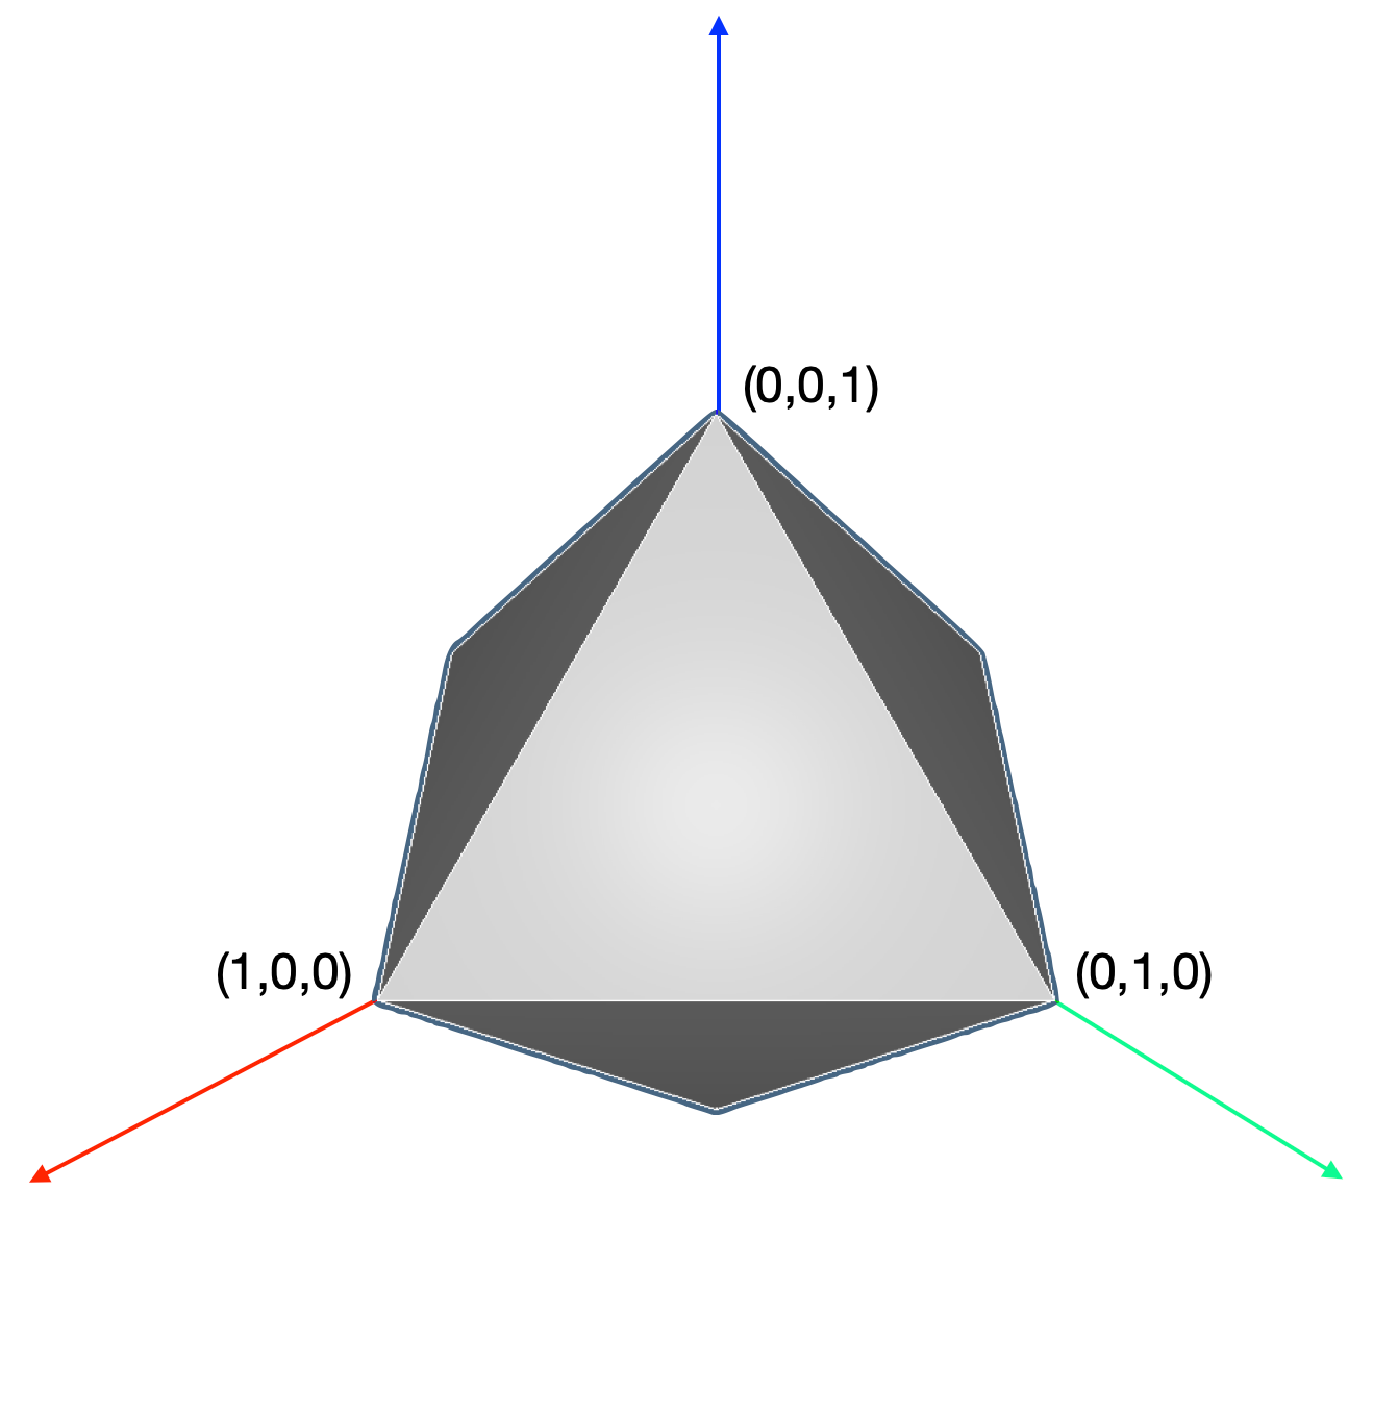
\includegraphics[width=\linewidth]{chapter-04/figs/octahedron} 
\end{minipage} \hfill
\begin{minipage}[c]{0.6\textwidth}
\begin{lstlisting}[language=JuliaLocal, style=julia, mathescape=true]
VIEW(octahedron::Hpc)
\end{lstlisting}
\caption{Plasm viewing generator expression. Remember that VIEW applies to Hpc values.}\label{fig:octahedron}
\end{minipage}
\end{figure}

\begin{coding}[The cellular complex]
Let’s note that the |octahedron::Hpc| is viewed, and that the |octahedron::Lar| is explored for stored data:\\
\begin{lstlisting}[language=JuliaLocal, style=julia, mathescape=true]
LAR(Octahedron).V 	#=
3×7 Matrix{Float64}:
  0.0  -1.0  0.0   0.0  1.0  0.0  0.0
 -1.0   0.0  0.0   0.0  0.0  1.0  0.0
  0.0   0.0  0.0  -1.0  0.0  0.0  1.0 	=#
LAR(Octahedron).C	#=
Dict{Symbol, AbstractArray} with 3 entries:
  :CV =) [[1, 2, 3, 4], [1, 3, 4, 5], [2, 3, 4, 6], [3, 4, 5,…
  :FV =) [[1, 2, 3], [2, 3, 4], [1, 3, 4], [1, 2, 4], [1, 3, …
  :EV =) [[2, 3], [1, 3], [1, 2], [3, 4], [2, 4], [1, 4], [3,…=#
\end{lstlisting}

For |$\#$C, $\#$F, $\#$E, $\#$V|, we see, looking at |.V| and |.C| above:
\begin{lstlisting}[language=JuliaLocal, style=julia, mathescape=true]
AA(LEN)(values(octahedron.C))'	#=
1×3 adjoint(::Vector{Int64}) with eltype Int64:
 8  20  18		=#
\end{lstlisting}
Therefore, we may see that the combinatorial (simplicial) complex corresponding to the 3D octahedron is made by 
8 + 20 + 18 + 7 = 53 cells of dimension 3, 2, 1, and 0, respectively (see Figure~\ref{fig:octahedron}).
\end{coding}




\subsection*{Shearing}
\label{s*ec:ccccccc}

In  a 2D elementary \emph{shearing tranformation} all points of each line (plane in 3D) orthogonal to a coordinate axis move by summing one (fixed) vector. The coordinate line (plane in 3D) remain fixed, and the translation vector change linearly with the distance of its line (plane) from the origin. Each of two elementary planar shearing depends on a single scalar parameter (the translation of the line at unit distance from the coordinate line). 

Each of the three elementary space shearing in 3D conversely depends on two scalar parameters (the coordinates of the planar translation vector of the plane at unit distance from the coordinate plane. Their 2D  and 3D matrices are as follows.

\[
\T{H}_x(h_x) = \mat{1\  & 0\\h_x & 1 },\qquad
\T{H}_y(h_y) = \mat{1\  & h_y\\0 & 1 };
\]
\[
\T{H}_x(h_y,h_z) = \mat{1 & 0 &  0 \\h_y & 1 & 0\\h_z & 0 & 1},\ 
\T{H}_y(h_x,h_z) = \mat{1 & h_x & 0 \\0 & 1 & 0\\0 & h_z & 1},\ 
\T{H}_z(h_x,h_y) = \mat{1 &  0 &  h_x\\0 & 1 & h_y\\0 & 0 & 1}.
\]

An elementary shearing differs from the identity matrix only for the elements of a single column, both in 2D and in 3D, and also in homogeneous 4D coordinates. 
In |Plasm|, the shearing tensor is named |H| and has the following semantics: first, indicate the column index; then give the $d-1$ ordered transformation parameters, i.e., one in 2D and two in 3D, some of which possibly zeros. Therefore we have |H(col)(pars)|.

\begin{figure}[htbp] %  figure placement: here, top, bottom, or page
\begin{minipage}[c]{0.35\textwidth}
   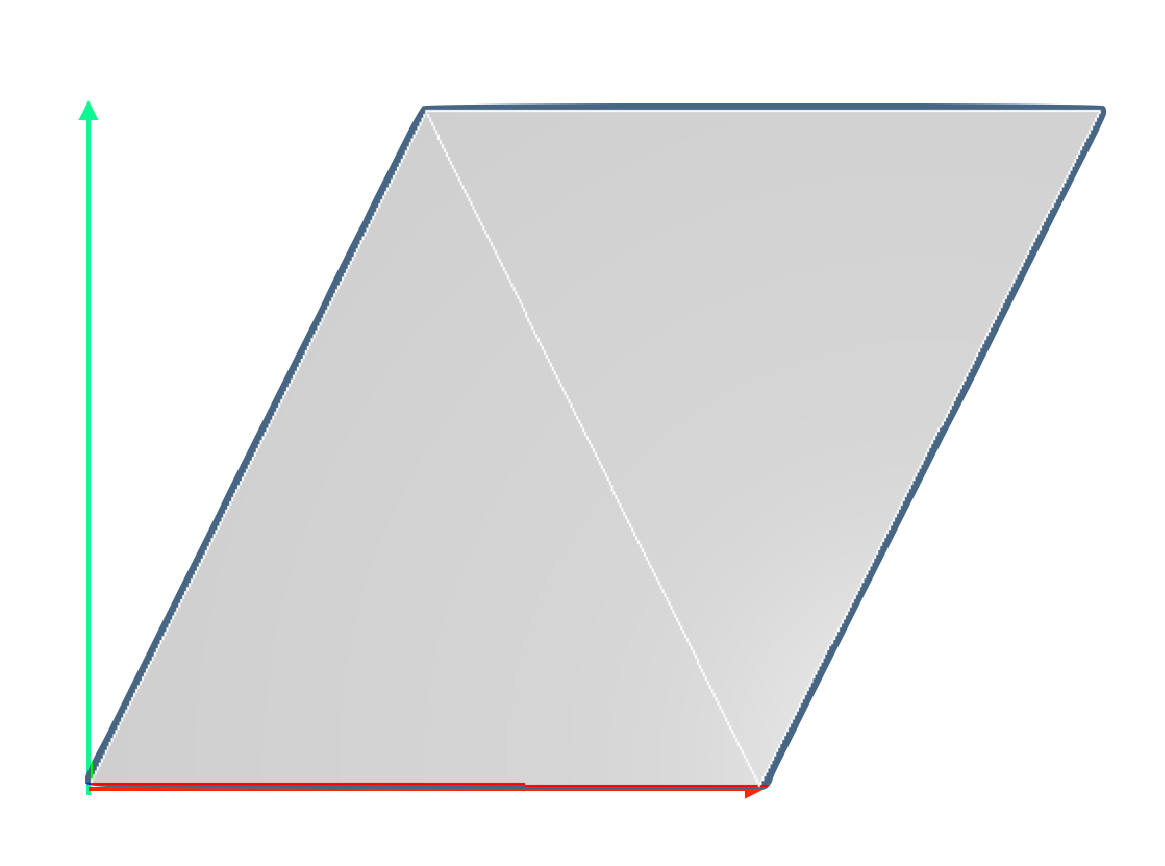
\includegraphics[width=\linewidth]{chapter-04/figs/shear2D} 
\end{minipage}\hfill
\begin{minipage}[c]{0.60\textwidth}
\begin{lstlisting}[language=JuliaLocal, style=julia, mathescape=true]
SQUARE(d) = CUBOID([d,d])
shearedsquare = H(2)(.5)(SQUARE(1))

VIEW(shearedsquare)
\end{lstlisting}
   \caption{Unit square sheared on the (second) coordinate $y$. The $y$ of model points does not change.}
\end{minipage}
\end{figure}

Typically, |shearing| is used by typesetting systems of computerized typography to get \emph{italic} versions of character fonts. Note also above how we define a parametric square (with a vertex on the origin).

\begin{figure}[htbp] %  figure placement: here, top, bottom, or page
\begin{minipage}[c]{0.35\textwidth}
   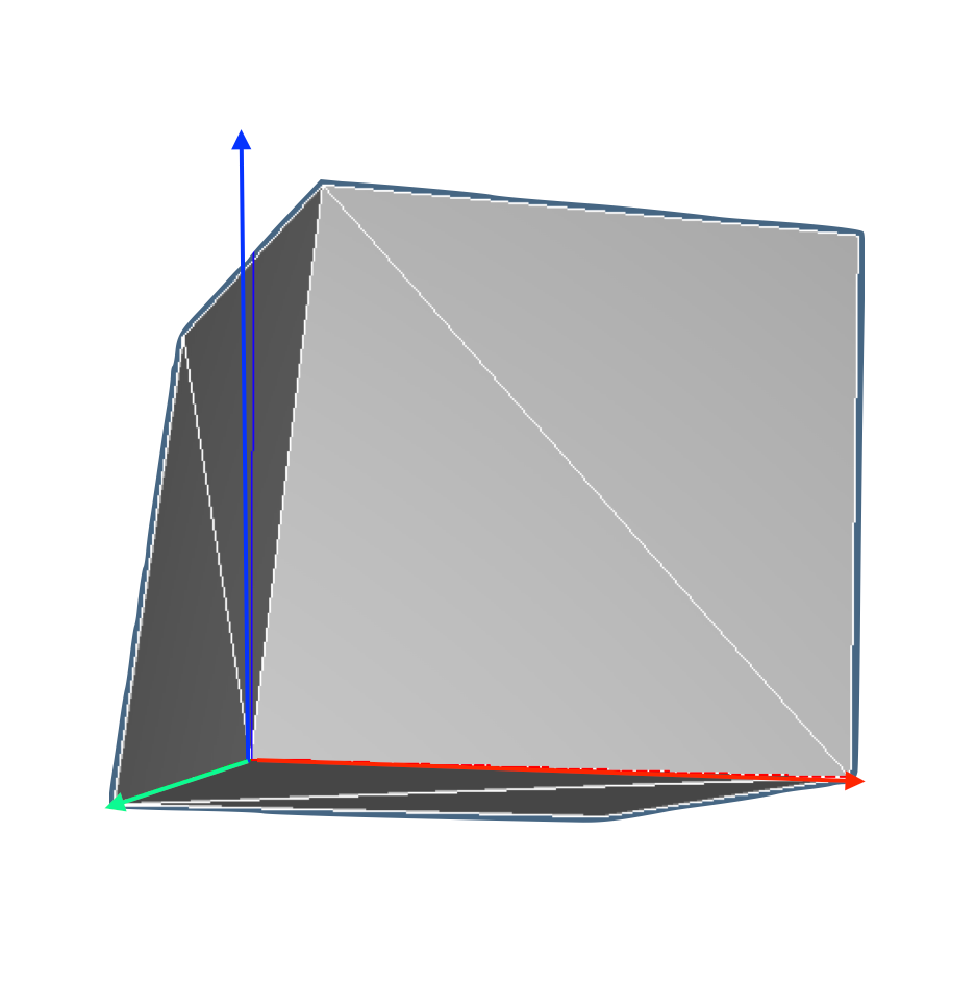
\includegraphics[width=\linewidth]{chapter-04/figs/shear3D} 
\end{minipage}\hfill
\begin{minipage}[c]{0.60\textwidth}
\begin{lstlisting}[language=JuliaLocal, style=julia, mathescape=true]
shearedcube = H(3)(.2,.3)(CUBE(1))

VIEW(shearedcube)
\end{lstlisting}
   \caption{Unit cube sheared on the (third) coordinate $z$. The $z$ of points do not change.}
\end{minipage}
\end{figure}

It is worthwhile to remark that the |H| mapping, as |R|, |GR|, |S|, |T|, |MAT|, and |HOMO| are dimension-independent, so can be applied to models of whatever embedding dimension $d$ of geometric models. Homogeneous \emph{normalized} matrices are used for implementation purpose. 


 
\subsection*{Translation}
\label{subsec:2:translation}

\begin{definition}[Translation transformation]
a translation is an invertible transformation of Euclidean space $\E^d$ generated by summing a fixed vector to all points.

A translation of plane $\mathbb{E}^2$ (or space $\mathbb{E}^3$) is not a linear transformation, since it moves the origin, but it is an \emph{affine} transformation, since all $\mathbb{E}^2$ (or $\mathbb{E}^3$) mapped points change by sum with a fixed vector (an \emph{affine action}). 
\end{definition}

Hence, a 2D or 3D translation depends on two (or three) scalar parameters, i.e., by the coordinates of the \emph{translation vector}.
We may therefore translate, using coordinates, a generic vector $\v{v} = (v_i)\in\mathbb{E}^d$:
\begin{equation}
\v{v}’ = \v{v} + \v{t}
\label{eq:vectortranslation}
\end{equation}
where $\v{t} = ({t}_i)$ is the translation vector, applied to all points in $\mathbb{E}^d$.




\subsubsection*{Translation in homogeneous coordinates}

The translation \ref{eq:vectortranslation} is reduced to a linear transformation and hence is representable by a product with a square matrix when using normalized homogeneous coordinates. Let’s remind our choice to use as homogeneous the first coordinate. 
For example, a translation of $\mathbb{E}^3$ is representable as
\begin{equation}
\T{T}(t_x,t_y,t_z) = \mat{1 & 0 & 0 & 0\\t_x & 1 & 0 & 0\\t_y & 0 & 1 & 0\\t_z & 0 & 0 & 1}
\end{equation}

We can see the equivalence between translation with Cartesian coordinates and homogenous normalized (affine) coordinates. Let $\v{v} = (x,y,z)$ be a point in 3D Euclidean space $\mathbb{E}^3$, and $\v{v}’ = (w=1,x,y,z)$ the same point in $\mathbb{R}^4$:
\[
\vet{x\\y\\z} + \vet{t_x\\t_y\\t_z} = \vet{x+t_x\\y+t_y\\z+t_z}
\qquad\mbox{and}\qquad
\mat{1 & 0 & 0 & 0\\
	t_x & 1 & 0 & 0\\
	t_y & 0 & 1 & 0\\
	t_z & 0 & 0 & 1} \, 
	\vet{1\\x\\y\\z} = \vet{1\\x+t_x\\y+t_y\\z+t_z}
\]

Just notice that a translation in 3D is actually a shearing $H_w(t_x,t_y,t_z)$ orthogonal to the added component in normalized homogeneous coordinates.

\begin{coding}[Translation of 3D geometric object] 
In |Plasm| we translate a geometric object of |Hpc| type via tensor application:

\begin{lstlisting}[language=JuliaLocal, style=julia, mathescape=true]
t_cube1 = T(1,2,3)(.5,.5,.5)(CUBE(1))
t_cube2 = T(3)(1)(CUBE(1))

VIEW(t_cube1);  VIEW(t_cube2)
\end{lstlisting}
A triple application of |T| function is needed: first to indices, then to translation paramenters, finally to the object of |Hpc| type to be translated.
\end{coding}

\begin{coding}[Parametric linear ladder stair] 
The |step| is a |Hpc| solid obtained by product of three line segments of given sizes.
An array of $n$ pairs |[move, step]| is generated and concatenated by the |CAT| operator.  Finally, the semantics of |STRUCT| aggregator combinator (see Section~\ref{sect:4-3}) produces the whole parametric object, shown in Figure~\ref{fig:stair}. 

\begin{lstlisting}[language=JuliaLocal, style=julia, mathescape=true]
function Ladder(lx,ly,lz, n)::Hpc
	step   = QUOTE(lx) * QUOTE(ly) * QUOTE(lz)
	move   = T(2,3)(0.8*ly, 0.8*lz)
	ramp   = STRUCT( CAT([[step, move] for k=1:n]) )
end #=
Ladder (generic function with 1 method)	=#
stair = Ladder(.8, .22, .18, 15);

VIEW(stair)
\end{lstlisting}

\end{coding}



\begin{figure}[htbp] %  figure placement: here, top, bottom, or page
   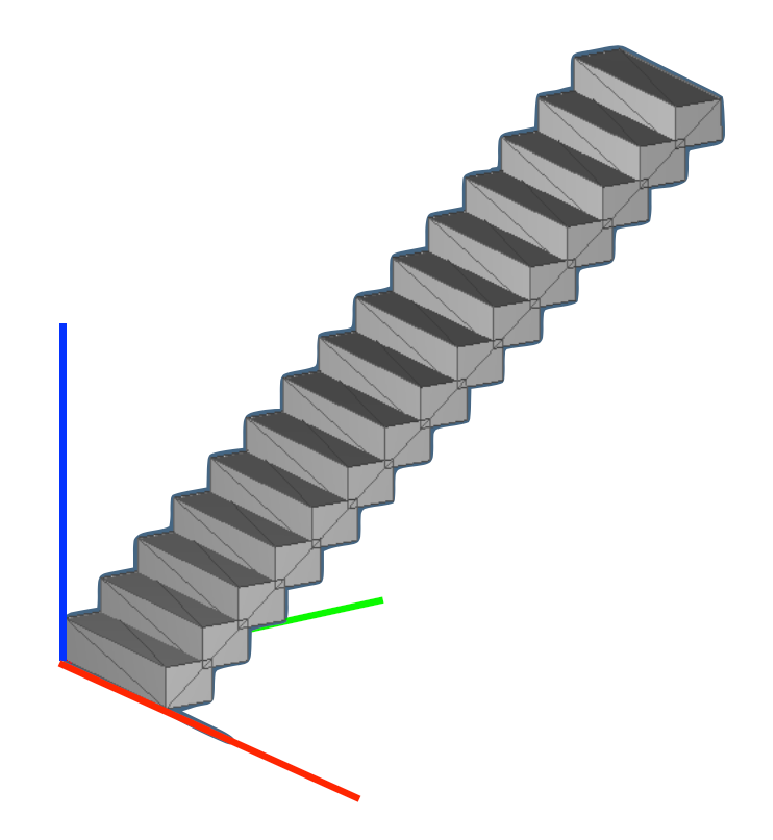
\includegraphics[width=0.35\linewidth]{chapter-04/figs/stair}
   \hspace{5mm}
   \sidecaption[t]
   \caption{Simple linear scale, demostrating an iterative use of tensors in {\small\sf STRUCT}. Of course, not only the number, but also the size and even the shape of {\sf step} model can be parametrized, as arguments of a geometric function returning {\sf Hpc} objects.}
   \label{fig:stair}
\end{figure}  






\section{Assembly of geometric objects}\label{sect:4-3}

Complex shapes are usually defined as hierarchical assemblies of either geometric primitives or more  complex shapes, each defined in a local coordinate system. 

Most graphics and modeling systems implement this semantics as a tree or \emph{hierarchical graph}, where affine geometry within the \emph{nodes} is defined in local coordinate frames, and arcs are associated to affine transformations that move the whole subgraph rooted in the ending node onto the coordinate system of the first node of the arc. The very first node is called \emph{root} of the data structure.


\subsection{Hierarchical graphs}

Acyclic graphs/multigraphs are also called \emph{hierarchical graphs}, because can be associated to a tree, generated at run-time by visiting the graph with some standard traversal algorithm~\cite{10.5555/1614191}, e.g., with a depth-first-search (DFS).  The ordered sequence of nodes produced by the traversal is sometimes called a \emph{linearized graph}.  Each node in this sequence is suitably transformed from local coordinates to \emph{world coordinates}, i.e. to the coordinates of the root, by the traversal algorithm.

The main ideas concerning \emph{scene graphs} can be summarized as
follows.
Nodes are  \emph{containers} of geometrical datasets stored in
\emph{local} coordinates.  Nodes are also used and implemented as root of subgraphs, 
whose data are transformed to the node coordinates by a traversal
algorithm.
Arcs $(a,b)$ are associated with affine transformations, which map the
data contained in $b$ from their local coordinates to the coordinates
of $a$.  More than one arc may exist between the same node pair.  This
allows storage in memory only of \emph{one copy} of each container.
The composite transformations of coordinates applied to the linearized
graph generated at traversal time are collectively known as the
\emph{modeling transformation}.


\subsection*{Object Transform}\label{sect:4-3-1} Any |Plasm| geometric value of |Hpc| type can be affinely transformed by direct application of an affine tensor to it.

\begin{coding}[Direct use of Tensor]\ 
Let’s combine with other language tensors, while generating the translated 1-skeleton of a cube:
\begin{lstlisting}[language=JuliaLocal, style=julia, mathescape=true]
SK = SKELETON;
translatedcube = (SK(1) ∘ T(1)(1) ∘ CUBE)(1);
\end{lstlisting}
\end{coding}

\begin{coding}[Example.2]\ 
Then, aggregate two objects into a single object within the \emph{same} coordinate frame:
\begin{lstlisting}[language=JuliaLocal, style=julia, mathescape=true]
singleframe = STRUCT(cube, tetra);
VIEW(singleframe)
\end{lstlisting}
\end{coding}

\begin{coding}[Example.3]\ 
\emph{Direct} application of tensor |T$_z$(1)|, followed by application of |R$_z$(-π/2)| to |tetra| value, which changes accordingly:
\begin{lstlisting}[language=JuliaLocal, style=julia, mathescape=true]
doubleframes = STRUCT(cube, (R(1,2)(-π/2) ∘ T(3)(1.0))(tetra) 
VIEW(doubleframes)
\end{lstlisting}
\end{coding}

\begin{coding}[Example.4]\ 
Exactly the same effect could be obtained by the following expression, because \emph{a transformation tensor is implicitly applied to every geometric value following it} in the parameter sequence of a |STRUCT| combinator. Evaluation is right-to-left, according to math composition rule:
\begin{lstlisting}[language=JuliaLocal, style=julia, mathescape=true]
doubleframe = STRUCT(cube, R(1,2)(-π/2), T(3)(1), tetra )
\end{lstlisting}
\end{coding}

\subsection*{Assembly of components}\label{sect:4-3-2}

Hierarchical models of complex assemblies are generated by aggregation of cellular complexes, each one defined in a local coordinate system, and possibly
relocated by affine transformations of coordinates.  This operation may be repeated
hierarchically, with subassemblies defined by aggregation of simpler parts, and so
on, until to have a set of leaves holding primitive models, which cannot be further decomposed.

Two main advantages can be found in a hierarchical modeling approach. Each component complex  and each partial assembly, at every hierarchical level, are defined independently from each other, using their |PROPERTIES| and local coordinate frame, suitably chosen to make the  definition easier.
Furthermore, only one copy of each component is stored in memory, and may be instanced
in different locations and orientations how many times it is needed.

\begin{figure}[htbp] %  figure placement: here, top, bottom, or page
   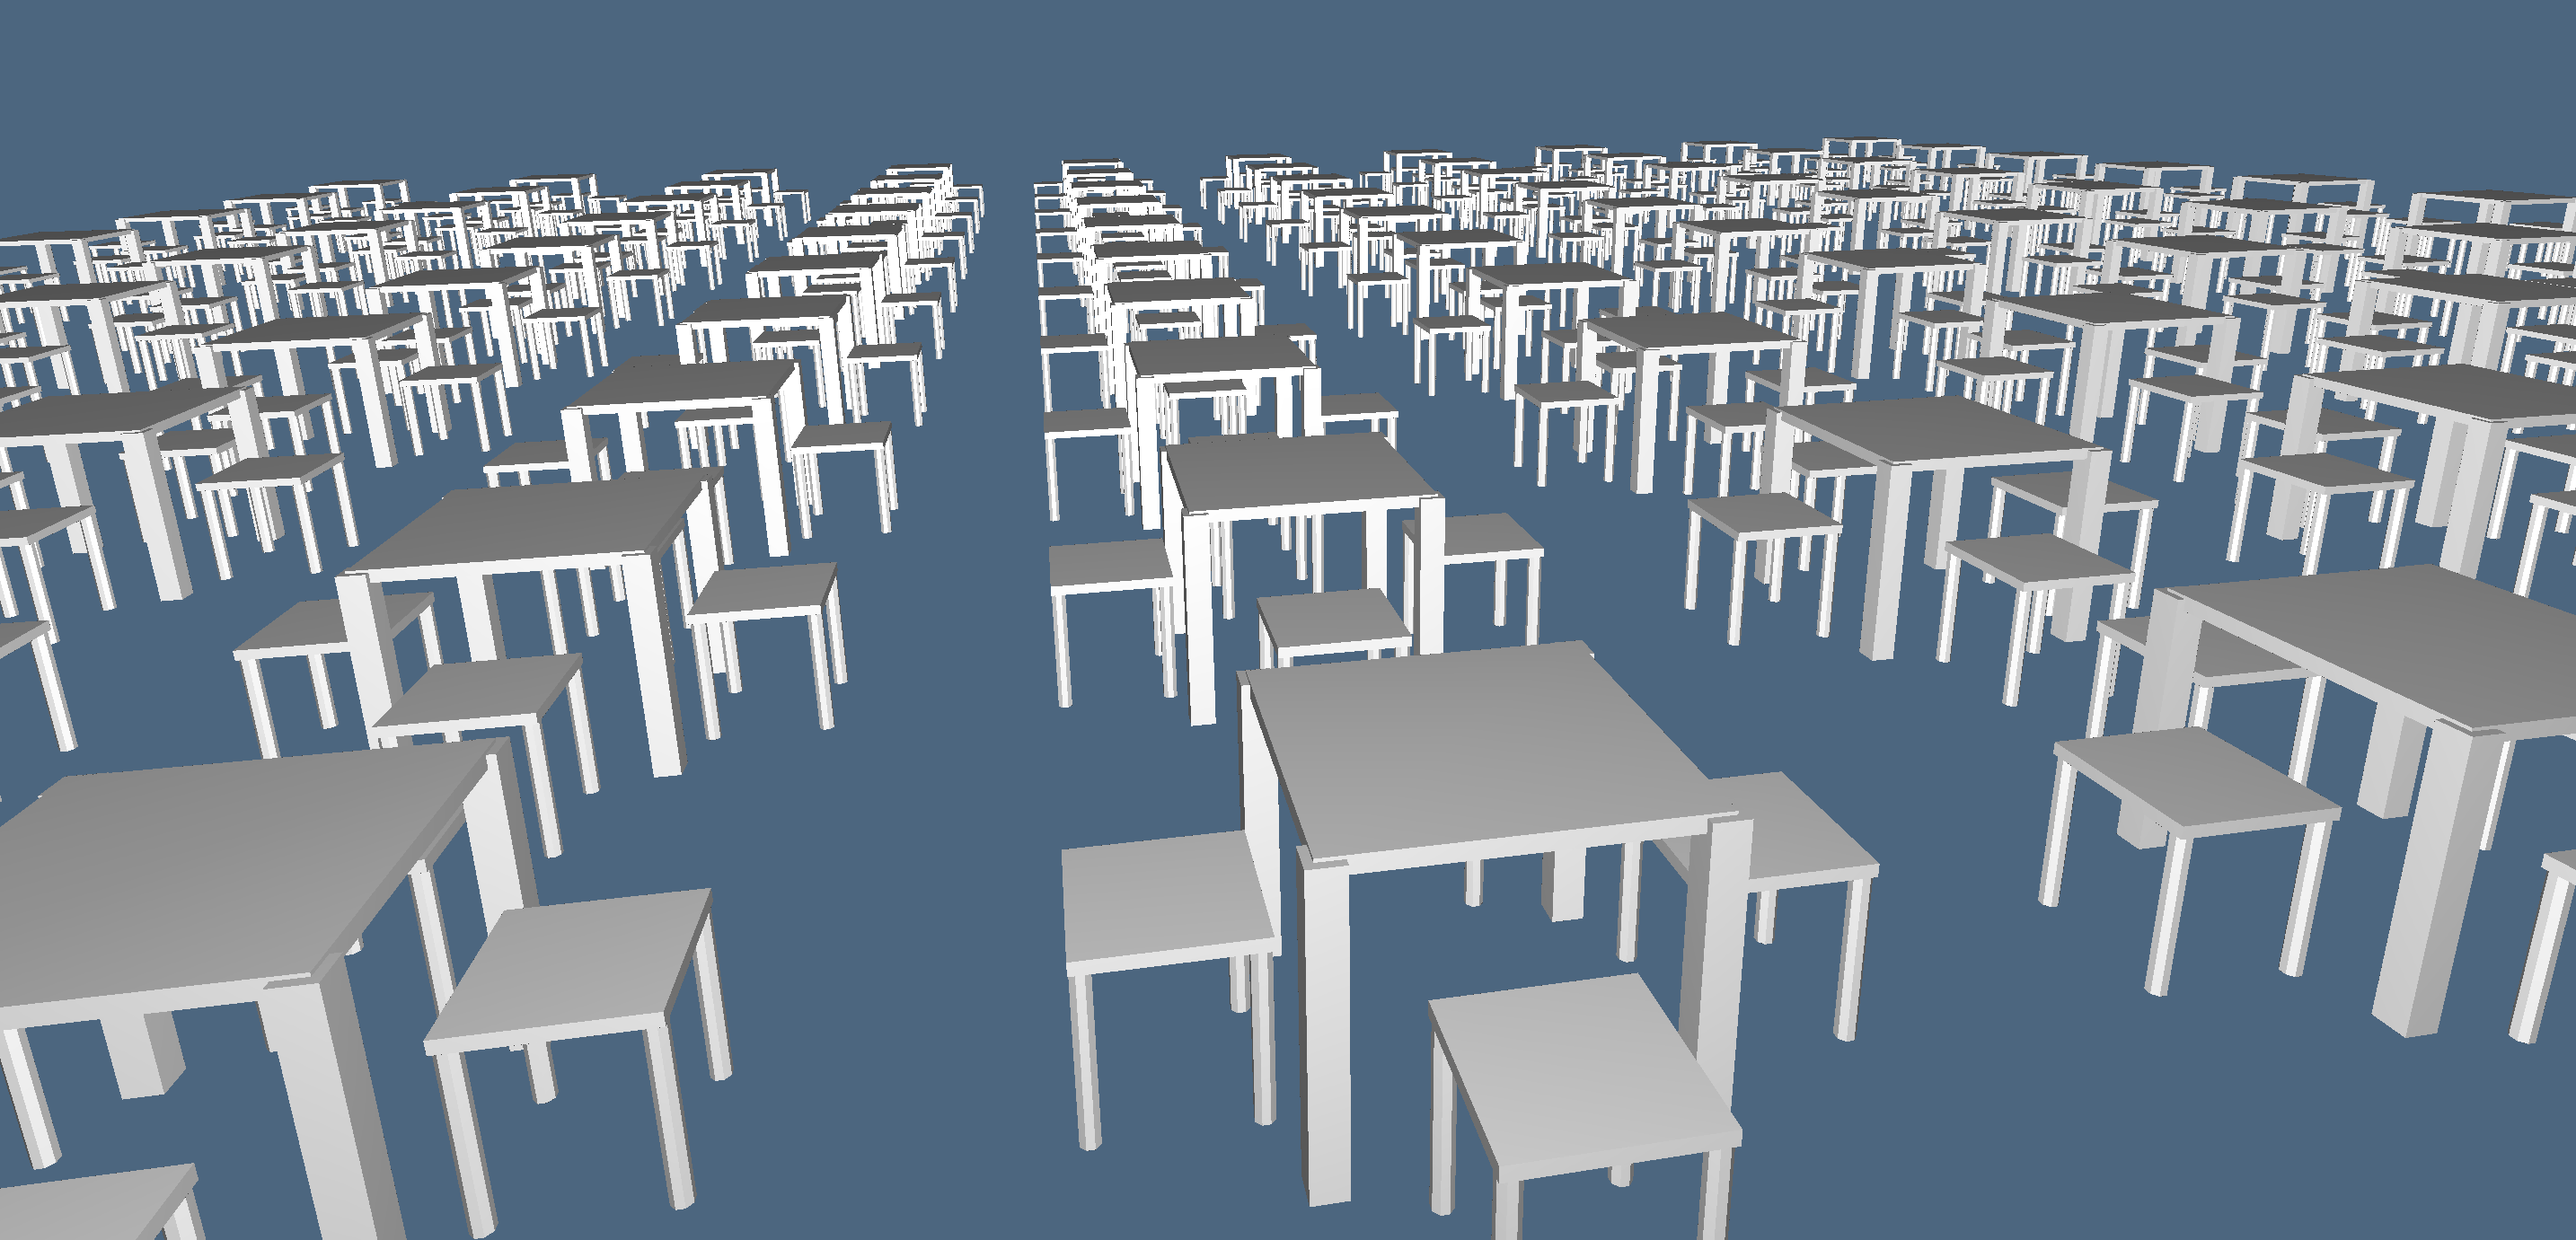
\includegraphics[width=\linewidth]{chapter-04/figs/refectory.png}
   \hspace{5mm}
   \caption{Hierarchical assembly of cellular 3-complexes.}
   \label{fig:refectory}
\end{figure}  


\subsubsection*{Directed Acyclic Graph (DAG)}\label{sect:4-3-2-1}

A \emph{hierarchical model}, defined inductively as an assembly of component parts,
is described by an \emph{acyclic directed multigraph}, often called a \emph{scene graph} or \emph{hierarchical structure} in computer graphics and modeling.  The main algorithm with hierarchical assemblies is the \emph{traversal} function, which transforms every component of the assembly from \emph{local coordinates} to global coordinates, often called \emph{world coordinates}.

\begin{definition}[Directed graph] A directed graph $G$ is a pair $(N,A)$, where
$N$ is a set of \emph{nodes} and $A$ is a set of directed \emph{arcs}, given as ordered pairs of nodes.  
\end{definition}
Such a definition is not sufficient when more than one arc must be considered
between the same pair of nodes.
The notion of \emph{multigraph} is hence introduced.  
In a multigraph, the same pair of nodes can be connected by multiple arcs.

\begin{definition}[Directed multigraph] A directed multigraph is a
triplet $G := (N,A,f)$ where $N$ and $A$ are sets of nodes and arcs, respectively, and $f:
A \to \mathbf{N}^{2}$ is a mapping from arcs to node pairs.  
\end{definition}

Directed graphs or multigraphs are said to be \emph{acyclic} when they do not contain cycles, i.e. when no path starts and ends at the same vertex.  \emph{Trees} are common examples of acyclic graphs. A tree, where each non-leaf node is the root of a subtree, is the best model of the concept of \emph{hierarchy}. Nodes in a tree can be associated with their integer \emph{distance} from the root, defined by the number of edges on the unique path from the root to the node.  A tree can be layered by \emph{levels}, by putting in the same subset (level) all the nodes with equal distance from the root.

\subsubsection*{Hierarchical structures in Plasm}\index{Hierarchical!structures in Plasm}


A \emph{container} of geometrical objects is defined in |Plasm| by
applying the combinator |STRUCT| to the contained objects' sequence (or array).  The value returned from the function application is of type 
\emph{hierarchical polyhedral complex} |Hpc|.  The coordinate system used by
the returned value is the one associated with
the first geometric object of the argument sequence.  

The resulting geometrical value is often associated with a variable used as the container's name, as in
\begin{lstlisting}[language=JuliaLocal, style=julia, mathescape=true]
    obj = STRUCT( obj$_{1}$, obj$_{2}$, $\ldots$, obj$_{n}$ ); VIEW(obj)
\end{lstlisting}

The |obj| geometry can be pictorially described, using the
previously discussed graph model of hierarchical structures, as shown
in Figure~\ref{fig:4:struct1}a.  Clearly, each component object may in
turn be defined as a container of other objects, i.e.~as the root of a
subgraph, as shown as shown below:
\begin{lstlisting}[language=JuliaLocal, style=julia, mathescape=true]
    obj$_2$ = STRUCT( obj$_{21}$, $\ldots$, obj$_{2m}$ )
\end{lstlisting}


\begin{figure}[htbp] %  figure placement: here, top, bottom, or page
   \centering
   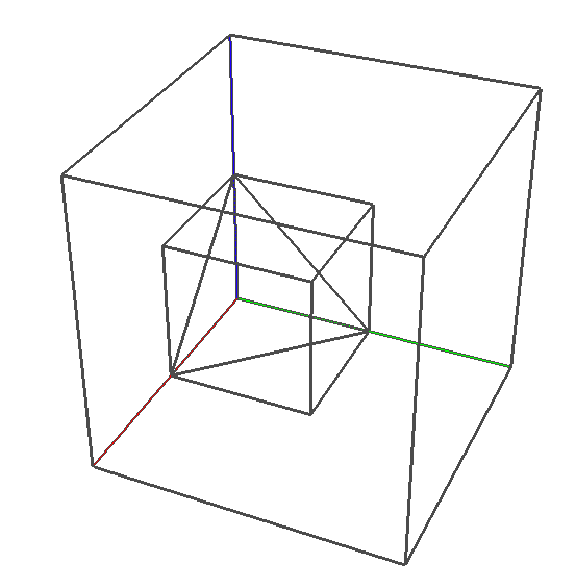
\includegraphics[width=0.3\linewidth]{chapter-04/figs/global} 
   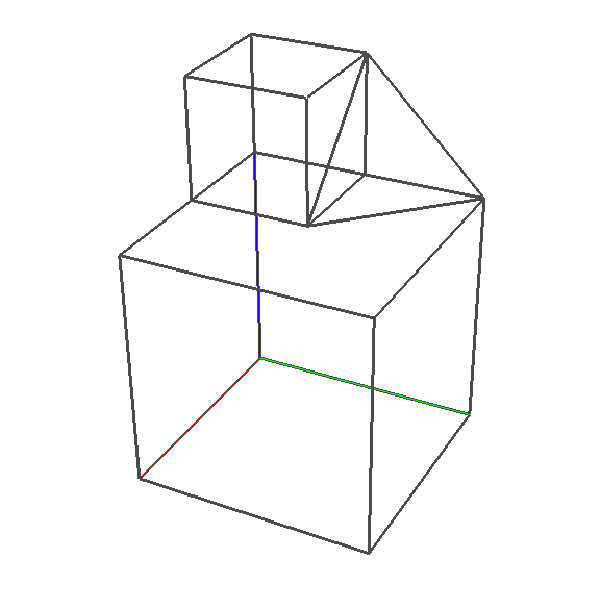
\includegraphics[width=0.3\linewidth]{chapter-04/figs/local} 
   \caption{Assembly by STRUCT: (a) without coordinate transformations. All three objects have the same origin;
    (b) with coordinate transformations.}
   \label{fig:4:struct1}
\end{figure}

Exactly the same geometric result would be generated by direct nesting of |STRUCT|
sub-expressions:
\begin{lstlisting}[language=JuliaLocal, style=julia, mathescape=true]
obj = STRUCT(obj$_1$, STRUCT(obj$_{21}$, $\ldots$, obj$_{2m}$) $\ldots$, obj$_n$)
\end{lstlisting}


The sequence argument of the |STRUCT| operator may either
contain or not affine transformations, together with polyhedral
complexes.  This fact results in generating an assembly either by
using the same (global) coordinates for the various components or by
using different (local) coordinate systems.  The two cases are
discussed in the two following subsections, respectively.

\subsubsection*{Assembly with global vs local coordinates}

Let’s assume that the sequence argument of a |STRUCT| expression
does not contain affine transformations. In other words, we assume
that the evaluations of the Plasm expressions in the argument sequence
only return polyhedral values.
In this case, the output polyhedral complex is returned within the
coordinate frame of the first element of the input sequence, and no
transformations of coordinates are applied to the assembly components,
which are only aggregated in the same space, as shown by the
the following example.

\begin{coding}[STRUCT assembly (1)]
The expression given below returns the
object of Figure~\ref{fig:4:struct1}a.  Note that the
three component shapes' local origin and coordinate axes
coincide.  The |SK(1)| operator (extraction of 1-skeleton)
was |$@1$|, not available in Julia, in classic |PlaSM|).
    
\begin{lstlisting}[language=JuliaLocal, style=julia, mathescape=true]
cube2, cube1, simplex = CUBE(2), CUBE(1), SIMPLEX(3)
obj1 = (SK(1) ∘ STRUCT)( cube2, cube1, simplex )
\end{lstlisting}
%obj1 = PROPERTIES(obj, Dict("line_width"=)3))
%VIEW(obj, Dict("background_color"=)[1,1,1]))
\label{ex:8:globalcoords}    
\end{coding}


\begin{coding}[STRUCT assembly (2)] \label{coding:4:2}
Here we aggregate the same geometric components used in
Coding~\ref{ex:8:globalcoords}, but also add up some
transformations of coordinates to the sequence of parameters of resulting assembly.
\begin{lstlisting}[language=JuliaLocal, style=julia, mathescape=true]
obj2 = (SK(1) ∘ STRUCT)(cube2, T(3)(2), cube1, T(2)(1), simplex)
\end{lstlisting}
%obj = PROPERTIES(obj, Dict("line_width"=)3))
%VIEW(obj, Dict("background_color"=)[1,1,1]))
\label{ex:8:localcoords}
The resulting geometric assembly is shown in \ref{fig:4:struct1}b.  
\end{coding}


\subsection*{STRUCT semantics}
\label{sec:8:localcoords}

We assume that in |Plasm|, the word \emph{tensor} stands for affine transformation.
Let’s suppose that tensors $|T|_k$ are contained
within the sequence argument of a |STRUCT| expression.
Each tensor in a |STRUCT| is applied to all polyhedral
complexes that follow it. The subsequent expressions are equivalent:

\begin{lstlisting}[language=JuliaLocal, style=julia, mathescape=true]
STRUCT( pol$_{1}$, T$_{1}$, pol$_{2}$, T$_{2}$, pol$_{3}$, $\ldots$ , T$_{n-1}$, pol$_n$ ) $\equiv$ 
STRUCT( pol$_{1}$, T$_{1}$(pol$_{2}$), (T$_{1}$$\sim$T$_{2}$)(pol$_{3}$), $\ldots$, (T$_{1}$∘T$_{2}$$∘\cdots∘$T$_{n-1}$)(pol$_{n}$)
\end{lstlisting}

Looking at the internal behavior of the geometric kernel of the
language, the following maps are applied to the |STRUCT|
application at evaluation time:

\begin{lstlisting}[language=JuliaLocal, style=julia, mathescape=true]
STRUCT( pol$_{1}$, (T$_{1}$ ∘ STRUCT)( pol$_{2}$, (T$_{2}$ ∘ STRUCT)( pol$_{3}$, $\ldots$ 
	(T$_{n-2}$ ∘ STRUCT)( pol$_{n-1}$, T$_{n-1}$(pol$_{n}$) ) $\ldots$ ) ) )
\end{lstlisting}

The above kind of evaluation (in DFS postorder) has inspired the actual implementation of the |Hpc| data structure.
Note, looking at the geometric result shown in
Figure~\ref{fig:4:struct1}b, that, according to Coding~\ref{coding:4:2}:
\begin{enumerate}
    \item
the output assembly is
represented in the coordinate system of first cube; 
    \item
the second cube is translated in $z$ direction; 
    \item
the unit tetrahedron is translated both in $z$ and in $y$ directions.
\end{enumerate}


\subsection*{Traversal algorithms}\label{sect:4-3-3}

There are many ways to visit (or walking) a graph or multigraph, traversing at least once every node or arc.
The \emph{traversal} of a hierarchical structure consists of a 
modified
\emph{Depth First Search} (DFS) of its acyclic multigraph,\footnote{
Notice that the standard \emph{dfs} graph traversal (see 
e.g.~\cite{AhoHopcroftUllman:DSA}) visits all the nodes once, since it works by
recursively visiting those sons of each node that it has not already 
visited. }
where each arc --- and not each node --- is traversed only once.  
% The
% traversal algorithm visits only one time all the edges, and is therefore executed in time
% \emph{linear} with the edge number.  Conversely, 
In particular, each node is traversed a number of times equal to the
number of different paths that reach it from the root node.

The aim of a traversal algorithm is to ``linearize" a 
structure network, by transforming all its substructures (i.e.~all the
subgraphs) from their \emph{local coordinates} to the coordinates of
the root node, assumed as \emph{world coordinates}.
% , as discussed in
% the following chapter, where the various coordinate systems used in a 
% \textsf{PHIGS}-like 3D pipeline are discussed.

For this purpose, a matrix denoted as the \emph{current transformation
matrix} (CTM) is maintained.  Such a CTM is equal to the product of
matrices associated with the arcs of the current path from the root to
the current node.  For the sake of efficiency, the traversal algorithm is
implemented by using a stack of CTMs.  When a new arc is traversed,
the old CTM is pushed on the stack, and a new CTM is computed by
(right) multiplication of the old one times the matrix of the arc. 
When unfolding from the recursive visit of the subgraph appended to the
arc,\footnote{Using a pictorial image, we could say: when the arc is
traversed in the opposite direction.} the CTM is substituted by the one
popped from the stack.  The \textsc{Traversal} algorithm is specified
in pseudo-language below.


\begin{script}[Traversal of a multigraph]
\begin{tabbing}
aaa\=aaa\=aaa\=aaa\=aaa\=aaa\=aaa\=aaa\=\kill
{\bf algorithm} \textsc{Traversal} ($(N,A,f): multigraph$) \+\\
   $CTM$ := identity matrix;\\
    TraverseNode ($root$)
\end{tabbing}


\begin{tabbing}
aaa\=aaa\=aaa\=aaa\=aaa\=aaa\=aaa\=aaa\=\kill
{\bf proc} \textsc{TraverseNode} ($n: node$) \+\\
  \textbf{foreach} $a\in A
  $ outgoing from $n$
  \textbf{do} \+\\
    TraverseArc ($a$); \\
  ProcessNode ($n$)
\end{tabbing}


\begin{tabbing}
aaa\=aaa\=aaa\=aaa\=aaa\=aaa\=aaa\=aaa\=\kill
{\bf proc} \textsc{TraverseArc} ($a=(n,m): arc$) \+\\ 
  Stack.push ($CTM$);\\
  $CTM$ := $CTM * a$.mat;\\
  TraverseNode ($m$);\\
  $CTM$ := Stack.pop()
\end{tabbing}



\begin{tabbing}
aaa\=aaa\=aaa\=aaa\=aaa\=aaa\=aaa\=aaa\=\kill
{\bf proc} \textsc{ProcessNode} ($n: node$) \+\\ 
  \textbf{foreach} object $\in$ $n$ \textbf{do} \+\\
    Process( $CTM * $object )
\end{tabbing}
\end{script}

\vspace{5mm}
The CTM is normally used to (left) multiply the vertices of geometric
objects stored in the traversed containers.  But the reader should
remember that equations of hyperplanes and normal vectors must be
conversely (right) multiplied for the inverse of the applied
transformation, according to the mapping of covectors discussed in
Section~\ref{subsec:6:actiononcovectors}.  A double stack of matrices,
where to push/pop both the CTM and its current inverse, may therefore
speed up the traversal.  As a result of the algorithm, a linearized model
in world coordinates is produced, which may be used, e.g., for rendering
purposes, as discussed in the next chapter.



\subsection*{Assembly examples}\label{sect:4-3-4}

The two examples given in this section are finalized to introduce some powerful |Plasm| higher-level functions and combinators. In particular, we use |STRUCT| and |MAP|, |CAT|, |DIESIS|, |PROPERTIES|, and |THINSOLID|. The geometric primitives |CUBE|, |CYLINDER|, and |SIMPLEX| are also used.

\subsubsection*{Refectory room model}\label{sect:4-3-4-1}

Some coordinated coding examples are given here, to show the development bottom-up of the geometric model of a refectory room with its main appliances, tables and user chairs. The room is visualized in Figure~\ref{fig:refectory}.

\begin{coding}[Table]\ 
Both the |tableTop| and |tablelegs| with $4$ |tableLeg| instances are generated starting from 3D cube of side 1:
\begin{lstlisting}[language=JuliaLocal, style=julia, mathescape=true]
cube = T(1,2)(-.5,-.5)(CUBE(1));
tableTop  = STRUCT( T(3)(.85), S(1,2,3)(1,1,.05), cube );
tableLeg  = STRUCT( T(1,2)(-.475,-.475), S(1,2,3)(.1,.1,.89), cube );
tablelegs = STRUCT( CAT(DIESIS(4)([tableLeg, R(1,2)(π/2)])) );
table = STRUCT( tableTop, tablelegs );
VIEW( table )
\end{lstlisting}
The operator |DIESIS| ($\#$) in old |Plasm| repeats 4 times its second argument.
\end{coding}

\begin{coding}[Chair]\ 
The |chair| object is made by a |chairTop| and 4 cylindrical |chairLeg| with radius |0.06| and height |0.5|:
\begin{lstlisting}[language=JuliaLocal, style=julia, mathescape=true]
cylinder  = CYLINDER([.06, .5])(8)
chairTop  = STRUCT( T(3)(0.5), S(1,2,3)(0.5,0.5,0.04), cube );
chairLeg  = STRUCT( T(1,2)(-.22,-.22), S(1,2)(.5,.5), R(1,2)(π/8), cylinder );
chairlegs = STRUCT( CAT(DIESIS(4)([chairLeg, R(1,2)(π/2)]) );
chair = STRUCT( chairTop, chairlegs );
VIEW( chair )
\end{lstlisting}
\end{coding}

\begin{coding}[Four sits]\  Four sits are produced by alternating chairs with local rotations in object |fourChairs|:
\begin{lstlisting}[language=JuliaLocal, style=julia, mathescape=true]
theChair   = STRUCT( T(1)(-.8), chair )
fourChairs = STRUCT( CAT(DIESIS(10)([R(1,2)(π/2), theChair]) );
fourSit    = STRUCT( fourChairs, table );
VIEW( fourSit )
\end{lstlisting}
\end{coding}

\begin{coding}[Single row of tables and chairs]\ 
The single 4-sit’s row is generated by alternating 10 instances 
of |fourSit| and T(2)(2.5) tensors:
\begin{lstlisting}[language=JuliaLocal, style=julia, mathescape=true]
singleRow = STRUCT( CAT(DIESIS(10)([fourSit, T(2)(2.5)])) );
VIEW( singleRow )
\end{lstlisting}
\end{coding}

\begin{coding}[Whole refectory]\ 
Analogously, the refectory room is furnished by juxtaposing 10 instances 
of |singleRow| and $x$-translations:
\begin{lstlisting}[language=JuliaLocal, style=julia, mathescape=true]
refectory = STRUCT( CAT(DIESIS(10)([singleRow, T(1)(3)])) );
VIEW( refectory )
\end{lstlisting}
\end{coding}

\subsubsection*{Plasm design of a turbo pump}\label{sect:4-3-4-1}

This section discusses the generation of a highly parameterized family of geometric objects stepwise. First, a code template |SOLIDHELICOID|, is given, and then a definitive model, |TURBOPUMP|, is produced. This is impossible to definie or build with the any |GUI|-based CAD system.

\begin{coding}[Solid helicoid]\ A parametric helicoid surface and solid follow. The source code represents a whole family of $\infty^6$ different shapes:
\begin{lstlisting}[language=JuliaLocal, style=julia, mathescape=true]
function SOLIDHELICOID(; nturns=3,R=1.,r=0.0,shape=[36*nturns, 8], pitch=2, thickness=0.1)
   totalangle = nturns*2*pi
   grid2D = INTERVALS(36*nturns)(36*nturns)*INTERVALS(4)(8)
   Domain2D=T(2)(r)(S(1,2)([totalangle/shape[1],R-r])(grid2D))
   surface = p-)((u,v)=p;[v*cos(u);v*sin(u);u*(pitch/(2*pi))])
   solidMapping = THINSOLID(surface)
   Domain3D = Domain2D * INTERVALS(thickness)(1);
   view = Dict("background_color"=)[1.,1,1])
   VIEW(MAP(surface)(Domain2D), view)
   VIEW(MAP(solidMapping)(Domain3D), view)
end;

julia) SOLIDHELICOID( r=0.4, thickness=0.2 )
\end{lstlisting}
\end{coding}

An atypical method was used in |SOLIDHELICOID| template, in order to |VIEW| both the first  step (a parametric surface), and the definitive parametric solid.
 
\begin{figure}[htbp] %  figure placement: here, top, bottom, or page
\centering
\begin{minipage}[c]{0.38\textwidth}
   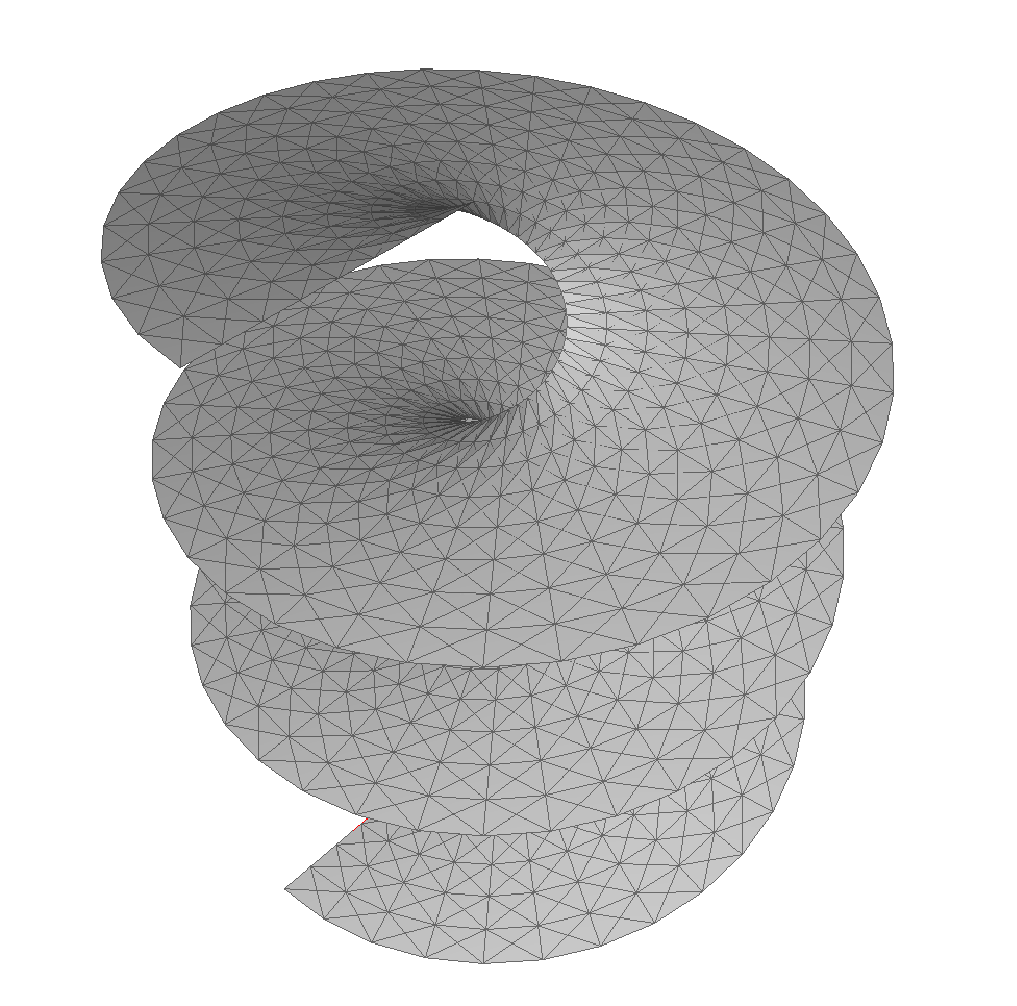
\includegraphics[width=\linewidth,height=\linewidth]{chapter-04/figs/surf-helicoid}%
\end{minipage}
\begin{minipage}[c]{0.38\textwidth}
   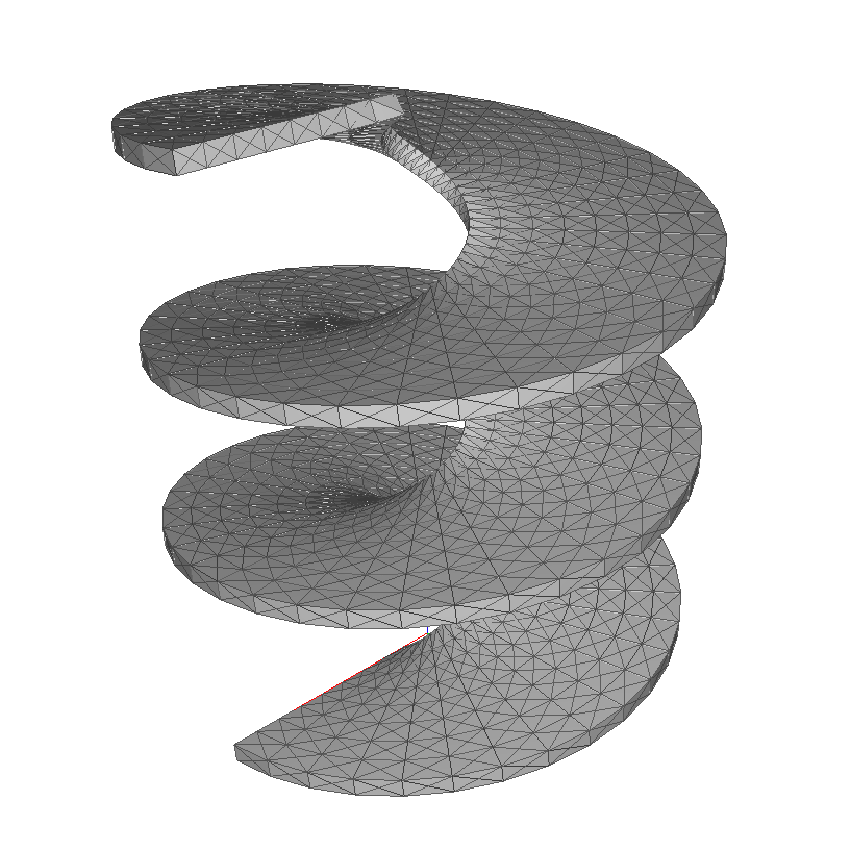
\includegraphics[width=\linewidth,height=\linewidth]{chapter-04/figs/solid-helicoid}%
\end{minipage}%
\caption{Parametrized helicoid values: (a) surface; (b) thin solid.}\label{fig:helicoid}
\end{figure}


\begin{coding}[Turbo pump]\ 
Starting
The main difference with |SOLIDHELICOID| template is the piecewise-linear |Dom2D| mapped from the rectangular |grid2D|.
\begin{lstlisting}[language=JuliaLocal, style=julia, mathescape=true]
function TURBOPUMP(; nturns=3, R=1., r=0.0, shape=[36*nturns,8], pitch=2, thickness=0.1)
   totalangle = nturns*2*pi;  xM = 36*nturns 
   (x0,xm1,xm2,xM) = (0.0, xM/2nturns, 6xM/2nturns, xM)
   G = (x-) x<xm1 ? x/xm1 : (x)xm2 ? 1+(xm2-x)/(xM-xm2) : 1))
   grid2D = INTERVALS(xM)(xM) * INTERVALS(1)(8)
   dom = MAP( p-)begin (u,v)=p; [u, (G(u)+0.1)*v] end )(grid2D)
   Dom2D= T([2])([r])(S([1,2])([totalangle/shape[1],R-r])(dom)) 
   surface = p-)((u,v)=p;[v*cos(u); v*sin(u); u*(pitch/(2*pi))]) 
   solidMapping = THINSOLID(surface)
   Domain3D = Dom2D * INTERVALS(thickness)(1)
   return MAP(solidMapping)(Domain3D)
end
\end{lstlisting}
\end{coding}


\begin{figure}[hbp] %  figure placement: here, top, bottom, or page
   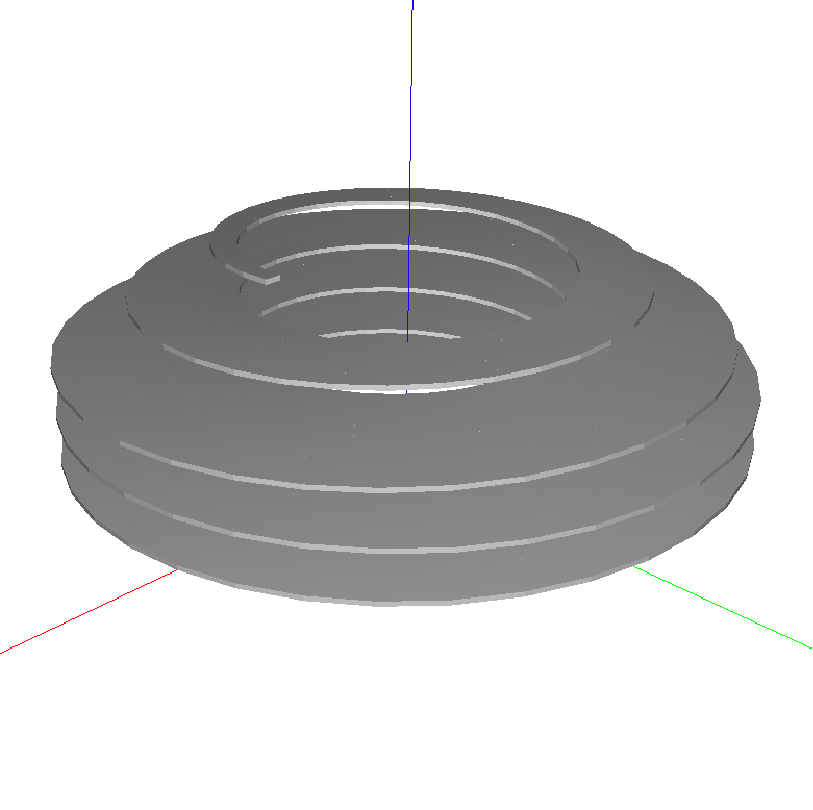
\includegraphics[width=0.337\linewidth]{chapter-04/figs/turbo-pump01}%
   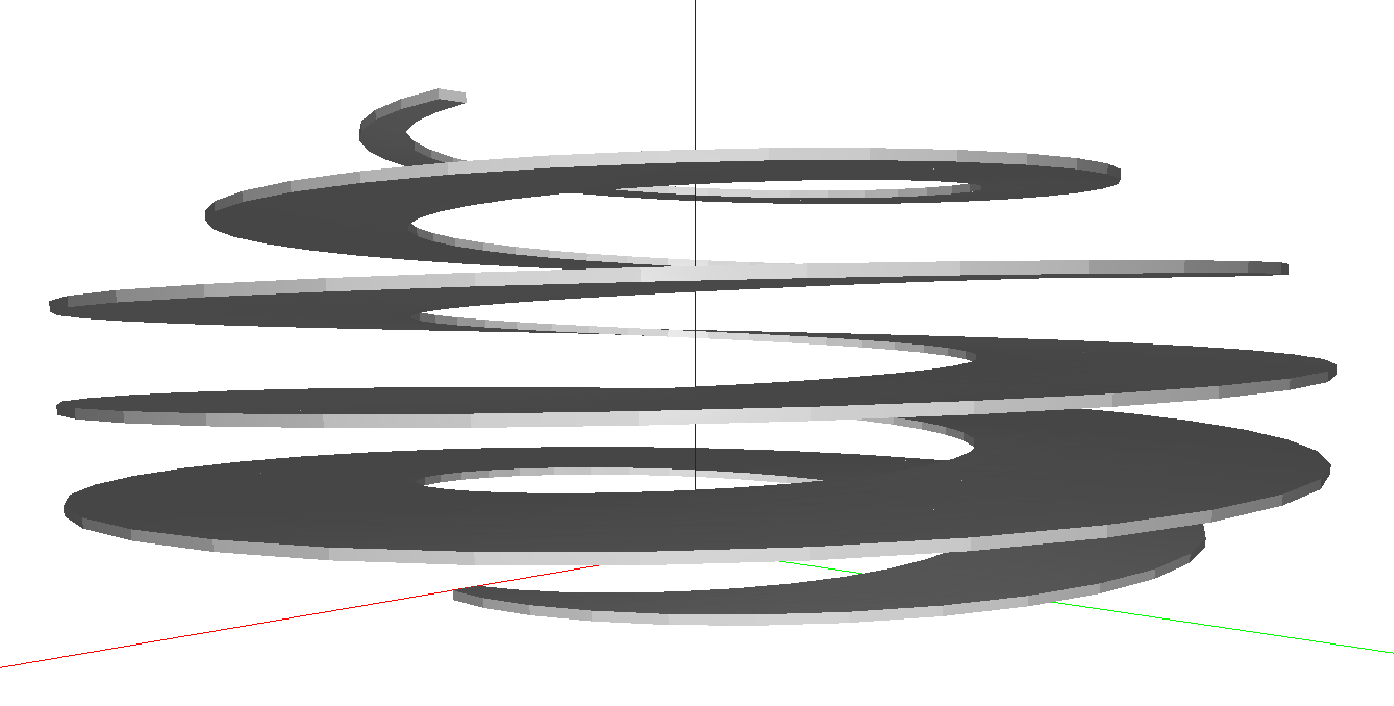
\includegraphics[width=0.663\linewidth]{chapter-04/figs/turbo-pump02}%
\caption{Two prospective images of the turbo pump component: (a) from top; (b) from side.}
\label{fig:turbopump}
\end{figure}

The piecewise linear |dom| shape is produced by the Julia function assigned to symbol |G|, implemented as a nested conditional triple statement. The three subdomain of piecewise |G| domain are defined by |(x0,xm1,xm2,xM)|.

\begin{coding}[Turbo pump’s object viewing]\ 
\begin{lstlisting}[language=JuliaLocal, style=julia, mathescape=true]
obj = TURBOPUMP( pitch=0.15, thickness=0.015, nturns=5, r=1/2 );
view = Dict("background_color"=)[1,1,1]); VIEW(obj, view)
\end{lstlisting}
The other parameters have default value, given in the definition head.
\end{coding}



\section{Attach properties to geometry}\label{sect:4-4}

Any geometric model is usually constituted by its geometry and associated properties or attributes that specify its appearance, like colors, textures, and materials used to render it on the screen or build a concrete instance in the real world. In this section, we shortly discuss some aspects of our interest: (a)~in XML, which was designed to describe the semantics of any kind of data in a computer; (b)  in the IFC standard, oriented to transport building data of architectural, engineering, and construction type between different computer systems. The section concludes with introducing the primitive |PROPERTIES| and |PropertySet| used by our Julia package |Plasm|.

\subsection*{XML Document Object Model (DOM)}\label{sect:4-4-1}

The eXtensible Markup Language (XML) is a software- and hardware-independent tool for storing and transporting data. An XML file is a text-based document that you can save with the |.xml| extension. 

Extensible Markup Language (XML) is a markup language used to describe the content and structure of the data in a document.
At the lemma XML of the Oxford English Dictionary~\cite{}, we find “a metalanguage which allows users to define their \emph{customized} markup languages, especially to display documents on the internet.”

\begin{definition}[Document Type Definition] 
DTD is a Document Type Definition. A DTD defines the structure and the legal \emph{elements} and \emph{attributes} of an XML document.
\end{definition}
XML was designed to carry data, hence with focus on what data are, and is extensible. This means that the author must define both the tags (markup) and the document structure.
The tags used in a document are not defined in any XML standard, but are “invented” by the author of the document.

\begin{definition}[XML Elements] are the basic building block of the XML document. It is used as a container to store text elements, attributes, media objects etc. 
Every XML documents contain at least one element whose scopes are delimited by start and end tags or in case of empty elements it is delimited by an empty tag.
\end{definition}

\begin{definition}[XML Attributes] XML elements can have attributes as sequences of pairs |name|=|”value”| separated by commas. Attributes are designed to contain data related to a specific element. Attribute values must always be quoted.
\end{definition}


\begin{definition}[XML Data Object Model (DOM) documents]
XML DOM documents are modeled using \emph{objects}, and the data model encompasses not only the structure of a document, but also the behavior of the document and the objects of which it is composed. 
\end{definition}

\begin{definition}[Structure Model] The term \emph{structure model} is used to describe the tree-like representation of a document. A tree structure contains a \emph{root} element (as parent), \emph{child} elements, and so on.
\end{definition}

The XML DOM defines also a standard way for accessing and manipulating files that presents an XML document as a tree-structure~\cite{}. 
Everything in such codified documents is a \emph{node}:
the entire document is a document node; every XML element is an element node; the text in the XML elements are text nodes; every attribute is an attribute node; comments are comment nodes. In particular, the DOM is a  language-independent standard API for how to get, change, add, and delete XML nodes.



\subsection*{IFC attributes and properties}\label{sect:4-4-2}

IFC (Industry Foundation Classes) is an Open Data schema and set of formats used to store OpenBIM data.  
The IFC file format and content is discussed in Chapter~\ref{chapt:8}. Some concepts are introduced here for reference and comparison with the definition of |Plasm| function |Properties|.  

\begin{definition}[IFC Entity]
The IFC Entity is a class of information defined by common attributes and constraints. 
It is similar to the term “class” in  programming languages but describing data structure only, not behavior such as methods. 
\end{definition}

All digital data objects in IFC belongs to an IFC class. 
\emph{Attributes} and \emph{properties} are two ways to assign extra metadata to an IFC class. Although they sound similar, they are not the same~\cite{}. 

The |IfcRoot| Entity is unique since it is the root of the information database and provides the four attributes |GlobalId|, |OwnerHistory|, |Name|, |Description|.
IFC classes can be divided into two categories: rooted and non-rooted classes. 
Rooted classes inherit attributes from |IfcRoot| Entity, whereas non-rooted classes do not. 

If a class is a subclass of another class, it inherits the same abilities of that class, such as having specific attributes, properties, or relationships. Subclasses \emph{do not} actually \emph{inherit the values} of the attributes themselves, but only the \emph{ability to have} that attribute. 


\subsubsection*{IFC attributes}\label{sect:4-4-2-1}



Each BIM (Building Information Model) object is assigned to a specific class (Entity), and each class has its attributes. Examples of attributes include Name, Description, PredefinedType, ObjectType, and Tag, where tag (or label) is the identifier at the occurrence level of the particular instance of a product or shape. All IFC classes have attributes. Attributes contain a name, as well as a value.  Attributes may be optional or mandatory. 

\begin{definition}[IFC Attribute]
is an unit of information within an entity, defined by a particular type or reference to a particular entity.
There are three kinds of attributes: \emph{direct}, \emph{inverse}, and \emph{derived} attributes, i.e., scalar values, queries for related data, or computations within the schema, respectively.
\end{definition}

The names of IFC Attributes are fixed, having been defined within the IFC standard. When an IFC class is defined, their attributes must be defined as well, or marked as empty if it is optional. The list of attributes that can be created for each IFC classes is fixed and specified in the IFC specification. 


\subsubsection*{IFC properties}\label{sect:4-4-2-2}

\begin{definition}[IFC Property]
The term “property” is a \emph{unit of information} that is dynamically associated with a particular entity instance, similar to "late-bound" or "run-time" in programming terminology. 
\end{definition}

This definition of “Property” is bound to “occurrence”, “template”, “set of occurrence”, set of “template”, meaning set of property templates serving a common purpose and having applicability to objects of a particular entity.

Unlike attributes, which are defined with each IFC class, properties themselves are an IFC class, and properties themselves have attributes. Also unlike attributes, related properties can be grouped into a |PropertySet|, or Pset, for short. This Pset can exist as its own IFC class, and then be linked to one or more relevant IFC classes. 


\subsection*{Plasm properties}\label{sect:4-4-3}

In |Plasm| we have functions objects and data objects. Every data object of geometric type |obj::Hpc| produced by a geometric |Plasm| function contains a possibly empty field |Properties::Dict{String, Any}| used to allocate a representation of any property, in particular of \emph{appearance} ones.  

Each |Hpc| value is a DAG (directed acyclic graph) node, root of the subtree whose children are mapped from the field |childs::Array|. The values of properties extend to the whole rooted subgraph, unless redefined locally.

The |childs| of a |Hpc| node may be either of |Hpc| or |Geometry| type. The |Geometry| node may have any subset of non-empty elements from:
\begin{lstlisting}[language=JuliaLocal, style=julia, mathescape=true]
points::Vector{Vector{Float64}}
edges::Vector{Vector{Int}}
faces::Vector{Vector{Int}}
hulls::Vector{Vector{Int}}
\end{lstlisting}
corresponding to 0-, 1-, 2-, and 3-dimensional (convex) cells, respectively. 

The |Plasm| type |Lar| is a flat version of |Hpc|+|Geometry|, allowing to make algebraic topological computations relative to the search of 3D atoms, that are B-reps of the basis  3-chain allowing to compute any symbolic form of the Boolean algebra induced by a collection of solid primitives (see Chapter~\ref{chapt:4}). 

Of course, there is no isomorphism between the two maps |Hpc|$\to$|Lar| and |Lar|$\to$|Hpc|.  In other words, their composition is not the identity map.

The standard properties of a value |obj::Lar| are the incidence relations between its cells, in either |Vector{Vector}| or in |SparseMatrix| form. In both case they can be extracted as |Dict| values associated to Julia’s symbol keys.


The predefined |Plasm| |PropertySet| are mostly related to graphics appearance, and in particular to the |mutable struct GLBatch|, used  by the module |Plasm/Viewer.jl| to send well-formed packets of graphical information to the GPU for rendering.

\begin{definition}[Appearance \sf PropertySet]
Currently, we have four classes of |PropertySet| to use (1) with general |Hpc| values (default); (2) with {\sf Viewer} objects (viewing); (3) when “exploding” assemplies of |Hpc|s (explode); (4) when showing a cellular complex annotated with cells indices (number).
\end{definition}

\begin{lstlisting}[language=JuliaLocal, style=julia, mathescape=true]
julia> typeof(PROPERTIES)
# typeof(PROPERTIES) (singleton type of function PROPERTIES, subtype of Function)

function PSET()  <: PROPERTIES end;
function PVIEW() <: PROPERTIES end;
function PEXPL() <: PROPERTIES end;
function PNUM()  <: PROPERTIES end;

function PropertySet() <: Union{PSET, PVIEW, PEXPL, PNUM} end 
# PropertySet (generic function with 1 method)
\end{lstlisting}

\subsubsection*{\small\sf PSET <: PROPERTIES}\label{4-4-3-1}

|PSET| is the default |PropertySet| associated to the appearance of any geometric value, either isolated of aggregated within a single root of |Hpc| type. 


\subsubsection*{\small\sf PVIEW <: PROPERTIES}\label{4-4-3-2}

|PVIEW| associates the default |PropertySet| to the interaction session, i.e., to the ability to handle joystick, keyboard, and mouse within a visualizer window containing an OpenGL context made available by the |ModernGL| package.


\subsubsection*{\small\sf PEXPL <: PROPERTIES}\label{4-4-3-3}

In order to manage a parametric explosion of a geometric object, defined as aggregation of simpler objects through a |STRUCT| primitive, we setup the |PEXPL| independent scaling parameters $s_x, s_y, s_z$ of each shape component’s centroid, either as 3-,  2-, and 1-cell complex. 



\subsubsection*{\small\sf PNUM <: PROPERTIES}\label{4-4-3-4}

Similarly to the previous case, the 
|PNUM| default |PropertySet| is used for the visualization of cells’ indices in  interaction sessions with a complicated geometric value, i.e., when looking at the text oindices of cells. It must specify a number of predefined properties concerning the size of text characters with respect to the bounding box size of current content of the viewing volume, as well as the colors and sizes of the different subsets of $d$-cells. 
The cell numbering is used for check and debug of geometric values. 


\section{Design documentation notebooks}\label{sect:4-5}

A virtual notebook environment is used for literate programming~\cite{10.1093.27.2.97}, a method of writing computer programs together with explanations and documentation, mostly using |Markdown| rich text~\footnote{Useful reference:\href{https://www.markdownguide.org/basic-syntax/}{https://www.markdownguide.org/basic-syntax/}.} in the last two decades. “Literate programming is a methodology that combines a programming language with a documentation language, thereby making programs more robust, more portable, more easily maintained, and arguably more fun to write than programs that are written only in a high-level language.”~\cite{Knuth:92}


A notebook is a computer document, specifically a file shareable with internet protocols, that merges source code, plain descriptions, data, and visualizations like function graphs and 3D models. It provides fast, shareable objects (files), to be used through an interactive environment, and useful for prototyping code, exploring and visualizing data, and sharing ideas with others.




\begin{figure}[htbp] %  figure placement: here, top, bottom, or page
   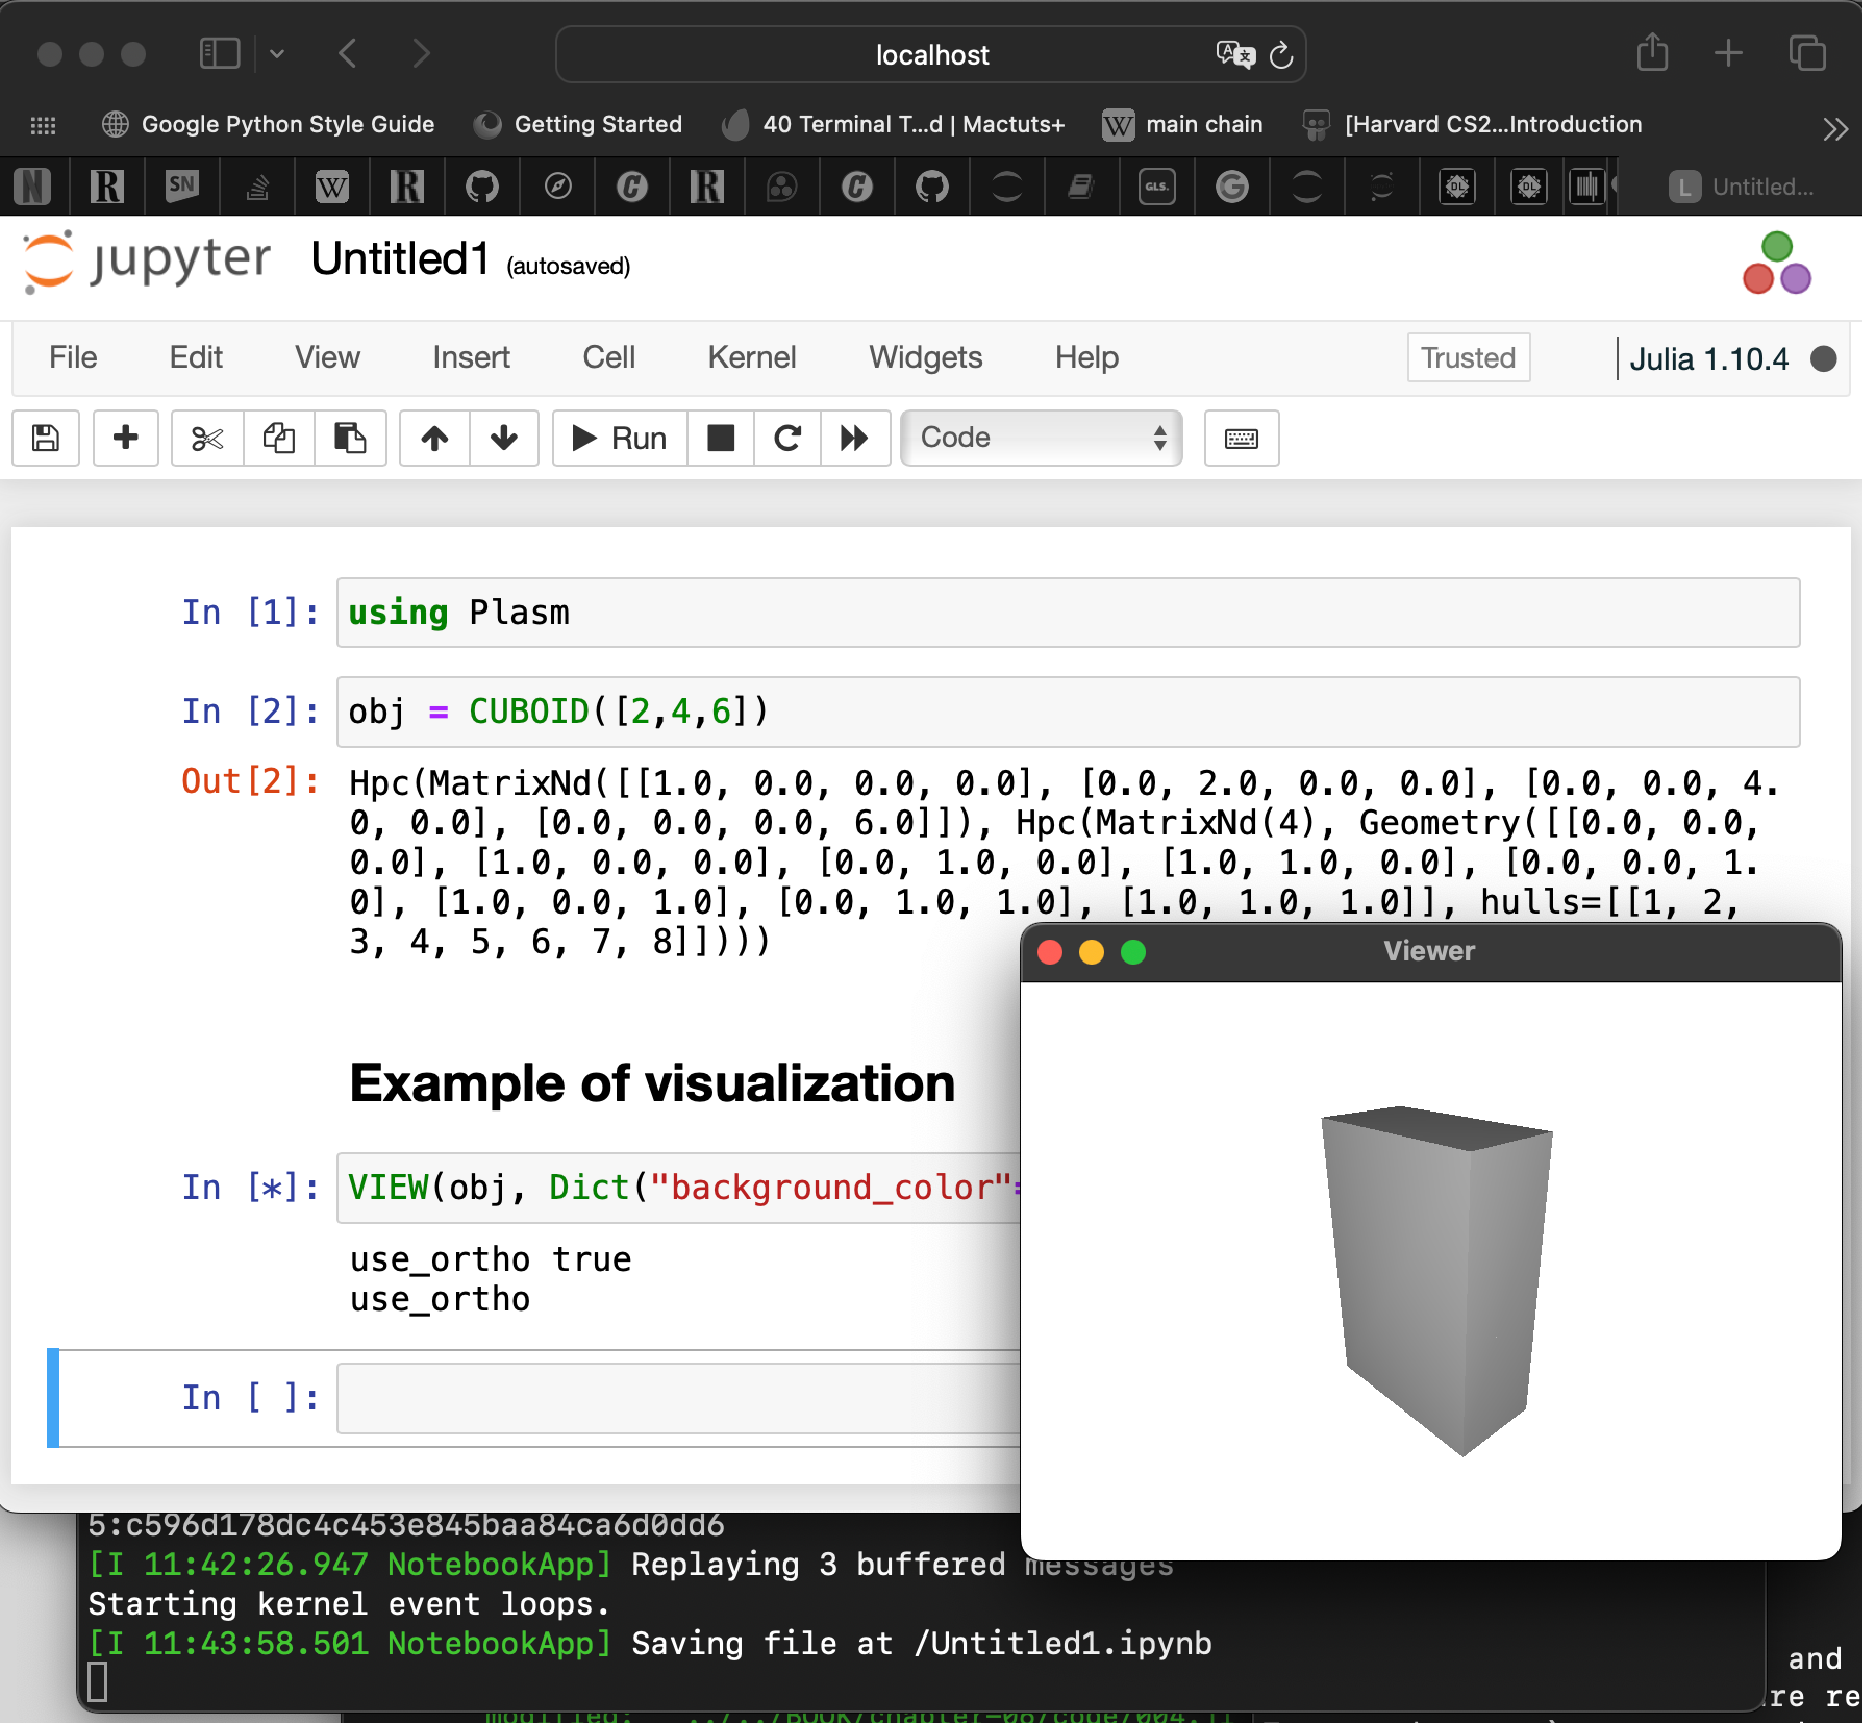
\includegraphics[width=\linewidth]{chapter-04/figs/jupyter}%
\caption{A small test session in Julia Jupiter using Plasm.}
\label{fig:jupyter}
\end{figure}


\subsubsection*{Install Julia notebook}\label{sect:4-5-1}


The Jupyter platform is a web-based interactive computing software. 
A Jupyter notebook is a web document (text file) with |.ipynb| sufffix.
The notebook combines live code, equations, narrative text, and 3D visualizations. It lets you run source code piece by piece, which is helpful when you're just imagining things and testing the ideas to develop with computer code, making it easier to understand what you're doing.
Project Jupyter's name refers to the three core programming languages supported by Jupyter: Julia, Python, and R. Currently, the Jupyter system supports over 100 programming languages, called "kernels" in the Jupyter ecosystem.

Julia Jupiter notebooks are very easy to install. 
Just write (the first time) to your Julia |REPL| console. 

\begin{lstlisting}[language=JuliaLocal, style=julia, mathescape=true]
julia> ]add IJulia 
\end{lstlisting}

When the package is installed, with |<backspace>| you will return to the standard |julia>| interactive mode.  Now write:

\begin{lstlisting}[language=JuliaLocal, style=julia, mathescape=true]
julia> using IJulia   

julia> notebook()
\end{lstlisting}
and wait few seconds. |Julia| will launch in background a |Jupyter| server and open a page on jour default web browser, asking to navigate the disk and either open a new file to work or one already existent and previously saved.


\subsubsection*{Install Julia Plasm package}\label{sect:4-5-1}

It is even more easier than the above; see Figure~\ref{fig:jupyter}. Of course, the output cell does not exists when the last line of code  terminates with a semicolon punctuation mark.

The reader should pay attention to some facts: (a) this notebook is a web document named |Untitled1.ipynb| and served locally from the machine’s |localhost|; (b) the language kernel (look top-right) is |Julia 1.10.4|; (c) the small circle close to it is black since the kernel has not already released control since the 3D window viewer is interactive; (d) it must be closed to go ahead; (e) the page is made by numbered |In| and |Out| cells, four of type |Code| and one of type |Markdown|; (f) an asterisk is on the right of the currently working cells.

\section{Export geometry}\label{sect:4-6}

There are several ways to export either produced or in-progress geometric |Plasm| models, starting from directly exporting the Julia sources. Depending on the size of the building project, the digital project evaluated within a short number of seconds of computing time could easily amount to datasets many hundreds of thousands of times more significant. 

Of course, the |Plasm| platform may also export/import Computer Graphics standard formats for polyhedral modeling, particularly using the boundary representation of the Boolean algebras’ atoms associated with the building design. The simplest options for file transport of geometry are boundary triangulations or polygons, directly representable through the |PolygonSet| entity primitives of the IFC file standard.

\subsubsection*{Direct export/import of sources}\label{sect:4-6-1}

Julia has two mechanisms for loading source code: \emph{code inclusion} and \emph{package loading}~\cite{}.
Code inclusion is relatively straightforward: it evaluates the given source file in the context of the caller process. It is good practice when writing a source file scheduled to export a geometric model (1) to choose a possibly long but semantically significant name and (2) to conclude each such file with one or more model |VIEW()|s of the exported building parts/aggregates. Inclusion also allows you to split a single program across multiple source files.

The expression |include("source.jl")| causes the contents of the file |"source.jl"| to be evaluated in the global scope of the module where the include call occurs. The expression |include()| can be called multiple times with the same file, and the file is evaluated every time. 

The second mechanism, \emph{package loading}, is more general and powerful. The |import <name>| or |using <name>| allows you to load a package—i.e., an independent, reusable collection of Julia code, wrapped in one or more module, and makes the resulting software library available by the name |<name>| inside the importing module~\cite{}. 

\begin{remark}
Creating a specialized Julia module or package for a specific architectural or engineering  project may be of great professional interest and economic satisfaction. 
E.g., the project could import Julia packages for the building typology under consideration, if any. In architecture, typology refers to identifying and grouping buildings according to their kind of use and similarity of essential characteristics, such as Residential, Educational, Institutional, Commercial, Business, or Industrial Buildings.
\end{remark}

\begin{remark}
You can have subtypes in each type with characteristic morphology: for example, in residential higher education, or in various types of specialty hospital establishment, which must follow strict legal requirements, and so on.
In addition, the specific design package might import parametric |Plasm| functions already developed for similar constructions and enrich them with new function methods finalized to the singular, unique design structure and shape under development.
\end{remark}

This kind of digital innovation process, on top of BIM and IFC standards (see Chapter~\ref{chapt:10}), could be of significant interest in case of development programs launched as sectorial construction interventions by governments (say housing, schools, etc.) or by charitable foundations in developing countries, where some standardization can greatly reduce the program costs.
 

\subsubsection*{Unevaluated/Evaluated/Binary LAR format}\label{sect:4-6-2}

Linear Algebraic Representation (|LAR|) is the name of the algebraic geometrical data structures and computational pipeline developed by the authors and others in the last decade, and embedded recently in |Plasm|. This data structure has various formats, depending on the advancement of computation. In particular, three LAR states may be expressed as unevaluated, evaluated, and binary.

\begin{description} 
\item[Unevaluated LAR] Sparse binary matrices that encode the cells of a cellular complex as incidence relations between $d$-cellls and $0$-cells ($0 \leq d \leq 3$). All the binary relations between cells of different dimensions can be easily generated. The occupied storage space is less or equal to that of common incidence structures in graphics and solid modeling.

\item[Evaluated LAR] is a pair (\emph{geometry}, \emph{topology}) where \emph{geometry} is the matrix |V::Matrix{Float64{| of coordinates of 0-cells (|V::Matrix{Float64}|), and \emph{topology} is a triple (in 3D) of sparse binary matrices, encoding the coboundary operators $\delta_0, \delta_1, \delta_2$ corresponding to incidence relations |VE|, |EF|, and |FC|. These result by the 3D algorithmic \emph{arrangement} pipeline that partitions the Euclidean 3-space on the boundary surfaces of any given collection of |Brep| solid models.

\item[Binary LAR] is the result of computation of the binary algebra induced by the spatial collocation and orientation of the whole collection of B-rep primitives and solids considered by the designer at the beginning of the computational pipeline, i.e., when all the geometric elements were collocated within the geometric design of the considered building portion. This binary matrix has number of columns equal to the number of computed atoms of the space arrangement and number of rows equal to the number of primitive shapes (of uniform material) used in a geometric design.
\end{description}

Every noteworthy subset of design atoms, selected by any reason---in particular, to assign material properties, catalog products, or compute volumes or cost---will be  extracted as a subset of corresponding columns and rows.

\subsubsection*{IFC PolygonSet file format}\label{sect:4-6-3}

Our preliminary tests showed that all the |Plasm| geometric shapes we defined or selected are exportable to transport file |IFC| as |PolygonSet| entities and their associated entities concerning polygons or triangles, vertex indices, and vertex coordinates. This point will be treated extensively in Chapter~\ref{chapt:10}.



% !TEX TS-program = xelatex

\chapter{Symbolic modeling with Julia Plasm}
\label{chapt:5}

Symbolic modeling is a semantic approach to knowledge representation and processing. A  symbolic approach to design with the aim of representing information and computation uses names to define the meaning of represented knowledge explicitly. The geometric knowledge is described here by Julia's names, which are chosen suitably for functionals, functions, formal and actual parameters, and finally for objects, fields, classes, attributes, methods, relations, etc. In this chapter, we give many examples of high-level Plasm programming, from topological, linear, and affine operators, to geometric mapping of complexes and grids to generate linearized approximation of curved manifold of intrinsic dimensions 1, 2, and 3. i.e., depending on such number of parameters; say, curves, surfaces, thin, and bulk solids.



\section{ Primitive generators}\label{sect:5-1}

Here, we introduce both single objects and aggregates of cells, typically by grid and mesh generators, resulting in a single |Hpc| value after the evaluation.


\subsection*{Higher order and partial functions}\label{sect:5-1-0}

As we have already seen in Section \ref{}, Julia |Plasm| is higher-level since allows for function that take functions as argument and/or may return a function value.  All functions are objects of Julia |Function| type. As objects (holding a reference to the function code), can be assigned to a name (identifier).

\begin{definition}[Function order] The \emph{order} of an object of |Function| type is the number of applications to actual parameters needed to return the ultimate actual value,  not a partial function value (needing further parameters).
\end{definition}

\begin{coding}[\sf  INTERVALS(size::Numrber)(n::Int)] In this example we show a second-order function (requiring two applications) that generates a 1D complex made by |n| line segments of total given |size| length.
\begin{lstlisting}[language=JuliaLocal, style=julia, mathescape=true]
segments = INTERVALS(10::Number)(4::Int)		#=
Hpc(MatrixNd(2), Geometry([[0.0], [2.5], [5.0], [7.5], [10.0]], hulls=[[1, 2], [2, 3], [3, 4], [4, 5]]))		=#
\end{lstlisting}
Note that |segments| value is 1D since its 11 vertices have one coordinate. 
\end{coding}


\begin{coding}[\sf  QUOTE(measures::Array{Number})]\
The formal parameter is an array of signed numbers.
\begin{lstlisting}[language=JuliaLocal, style=julia, mathescape=true]
two_aligned_segments = QUOTE([1,-2.5,1])			#=
Hpc(MatrixNd(2), Geometry([[0.0], [1.0], [3.5], [4.5]], hulls=[[1, 2], [3, 4]]))	=#
\end{lstlisting}
Positive numbers denote solid intervals of a given size; negative numbers denote hollow space, i.e., displacement of following segments. Successive negative numbers are allowed.\end{coding}


\begin{coding}[\sf  Q(measure::Number)]\
The formal parameter is a signed number. 
\begin{lstlisting}[language=JuliaLocal, style=julia, mathescape=true]
segment = Q(10)
Hpc(MatrixNd(2), Geometry([[0.0], [10.0]], hulls=[[1, 2]]))
\end{lstlisting}
A single |segment| of given size.
\end{coding}


\subsection*{Single convex cell}\label{sect:5-1-1}

Julia |Plasm| contains a great library of generator functions of very simple objects made by a single convex cell, and completely specified by its set of vertices only. 
Few examples follow; Other examples can be extracted or generated by the user looking at file |src/fenvs.jl|, including the Platonic solids. The multidimensional $d$-permutaheron is generated in Coding \ref{4-2-permutahedron}. 

\begin{coding}[\sf  CUBOID(size)]\
Multidimensional cuboid with |sizes::Vector{Number}|.
\begin{lstlisting}[language=JuliaLocal, style=julia, mathescape=true]
CUBOID([1])			#=
Hpc(MatrixNd(2), Hpc(MatrixNd(2), Geometry([[0.0], [1.0]], hulls=[[1, 2]]))) =#

CUBOID([1,2])			#=
Hpc(MatrixNd([[1.0, 0.0, 0.0], [0.0, 1.0, 0.0], [0.0, 0.0, 2.0]]), Hpc(MatrixNd(3), Geometry([[0.0, 0.0], [1.0, 0.0], [1.0, 1.0], [0.0, 1.0]], hulls=[[1, 2, 3, 4]]))) =#

CUBOID([1,2,3])			#=
Hpc(MatrixNd([[1.0, 0.0, 0.0, 0.0], [0.0, 1.0, 0.0, 0.0], [0.0, 0.0, 2.0, 0.0], [0.0, 0.0, 0.0, 3.0]]), Hpc(MatrixNd(4), Geometry([[0.0, 0.0, 0.0], [1.0, 0.0, 0.0], [0.0, 1.0, 0.0], [1.0, 1.0, 0.0], [0.0, 0.0, 1.0], [1.0, 0.0, 1.0], [0.0, 1.0, 1.0], [1.0, 1.0, 1.0]], hulls=[[1, 2, 3, 4, 5, 6, 7, 8]]))) =#

CUBOID([1,2,3,4])			#=
Hpc(MatrixNd([[1.0, 0.0, 0.0, 0.0, 0.0], [0.0, 1.0, 0.0, 0.0, 0.0], [0.0, 0.0, 2.0, 0.0, 0.0], [0.0, 0.0, 0.0, 3.0, 0.0], [0.0, 0.0, 0.0, 0.0, 4.0]]), Hpc(MatrixNd(5), Geometry([[0.0, 0.0, 0.0, 0.0], [1.0, 0.0, 0.0, 0.0], [0.0, 1.0, 0.0, 0.0], [1.0, 1.0, 0.0, 0.0], [0.0, 0.0, 1.0, 0.0], [1.0, 0.0, 1.0, 0.0], [0.0, 1.0, 1.0, 0.0], [1.0, 1.0, 1.0, 0.0], [0.0, 0.0, 0.0, 1.0], [1.0, 0.0, 0.0, 1.0], [0.0, 1.0, 0.0, 1.0], [1.0, 1.0, 0.0, 1.0], [0.0, 0.0, 1.0, 1.0], [1.0, 0.0, 1.0, 1.0], [0.0, 1.0, 1.0, 1.0], [1.0, 1.0, 1.0, 1.0]], hulls=[[1, 2, 3, 4, 5, 6, 7, 8, 9, 10, 11, 12, 13, 14, 15, 16]]))) =#
\end{lstlisting}
Cuboids of given sizes. Of course, the unit hypercube in $\E^6$ has |size = [1,1,1,1,1,1]|. 
\end{coding}

The |Plasm| coding of the “icosphere”, polyhedral approximation of the 2-sphere obtained by subdividing the |ICOSAHEDRON()| surface is given here, starting from the Platonic solid. The generation method is extremely simple. We obtain the vertices at step $i+1$ by adding to the vertices at step $i$ those obtained by subdivision of all edges. Ma make use of theHpc structure and the Lar structure.


\begin{coding}[\sf  ICOSPHERE(seed::Hpc)::Hpc]\
First we generate the cell complex of the input |obj| using the |LAR| combinator, then for each edge we compute the mean point, then we aggregate to the old vertices the new ones, scaled by the factor |r1/s1| built with the distance from |[0,0,0]| center of both models.
\begin{lstlisting}[language=JuliaLocal, style=julia, mathescape=true]
function ICOSPHERE(obj::Hpc)::Hpc
   W  = LAR(obj).V
   EV = LAR(obj).C[:EV]
   W  = [W[:,k] for k=1:size(W,2)]
   V  = [(W[v1]+W[v2])./2 for (v1,v2) in EV]
   r1 = sqrt(sum(W[1].^2))
   s1 = sqrt(sum(V[1].^2))
   CONVEXHULL([W; V*(r1/s1)]);
end
\end{lstlisting}
Finally, the |[W; V*(r1/s1)]::Vector{Vector{Float64}}| made by old vertices and by new scaled ones is given to the operator |CONVEXHULL| that transforms such a |Vector| of point (|Vector{Float64}|) in their geometric \emph{convex hull}.
Just remember that such polyhedra are convex sets, hence they have a \emph{single} (convex) cell. \begin{lstlisting}[language=JuliaLocal, style=julia, mathescape=true]
out0 = ICOSAHEDRON();   VIEW(out0)
out1 = ICOSPHERE(out0); VIEW(out1)
out2 = ICOSPHERE(out1); VIEW(out2)
out3 = ICOSPHERE(out2); VIEW(out3)
...		
\end{lstlisting}
Successive approximations of icosphere with 12, 42, 162, 600, etc., vertices.
Let’s remark the extreme simplicity of such polyhedral generations.
\end{coding}

\begin{figure}[htbp] %  figure placement: here, top, bottom, or page
   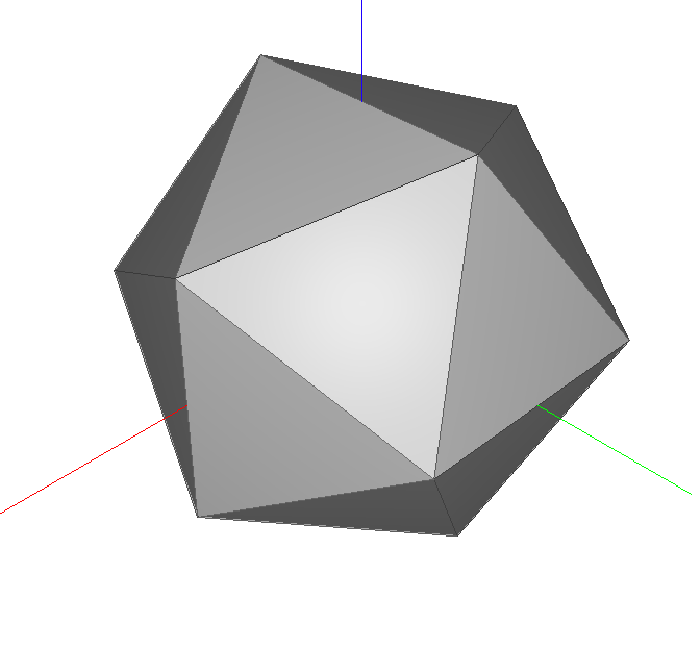
\includegraphics[width=0.34\linewidth]{chapter-05/figs/icosphere0}%
   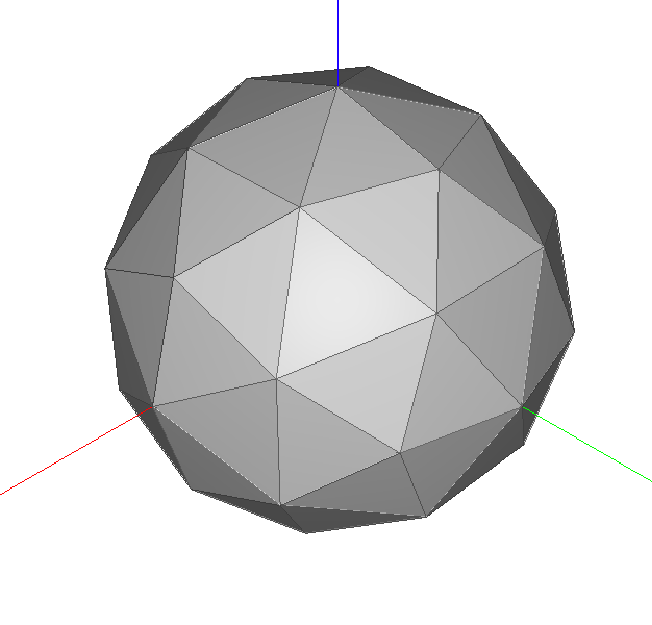
\includegraphics[width=0.33\linewidth]{chapter-05/figs/icosphere1}%
   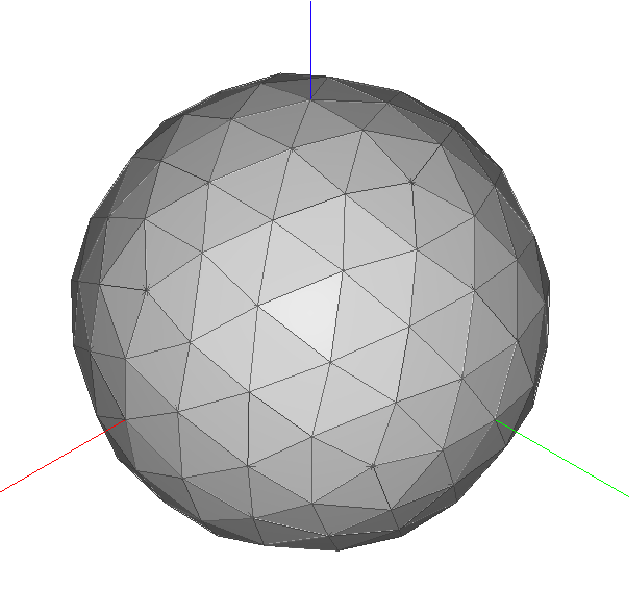
\includegraphics[width=0.325\linewidth]{chapter-05/figs/icosphere2}%
\hfill
\caption{(a) Icosahedron; (b) icosphere with 42 vertices; (c)  icosphere with 162 vertices. }
\label{5:icospheres}
\end{figure}



\subsection*{Multiple cell objects}\label{sect:5-1-1}


The functions |INTERVALS| or |QUOTE| may be used to create many types and patterns of grid geometries.

\begin{script}[Building frame]\
First we give the main dataset of a building frame, by “quoting” the side measures of 2D design plan:
\begin{lstlisting}[language=JuliaLocal, style=julia, mathescape=true]
# Longitudinal trusses
Y = QUOTE([0.3, -6, 0.3, -6, 0.3])
# transverse beams
X = QUOTE([0.3, -3, 0.3, -4.2, 0.3, -3, 0.3])
# vertical measurements
Z = QUOTE([3,0.3])
\end{lstlisting}
Then, an alternate set of |INTERVALS| vector parameters are generated by Julia broadcast |.*| of the scalar |-1|, in order to invert all the signs.
\begin{lstlisting}[language=JuliaLocal, style=julia, mathescape=true]
X1 = QUOTE([0.3, -3, 0.3, -4.2, 0.3, -3, 0.3].* -1)
Y1 = QUOTE([0.3, -6, 0.3, -6, 0.3].*-1)
Z1 = QUOTE([3,-0.3].*-1)
\end{lstlisting}
Below, the 3D |frame| subsystems are generated. They are the $C_3$ basis of a local cellular complex. Note the variation pattern at |trusses1|.
\begin{lstlisting}[language=JuliaLocal, style=julia, mathescape=true]
# Cartesian product
pillars = COLOR(RED)(X*Y*Z);
trusses = COLOR(YELLOW)(X*Y1*Z1);
trusses1 = COLOR(YELLOW)(X1*Y*QUOTE([-2.7,0.6]));
floorslab = COLOR(GREEN)(X1*Y1*Z1);
\end{lstlisting}
Finally, the sub-complexes of 3D cells are aggregated in a single |Plasm| complex using the |STRUCT| combinator discussed in the next session. Let us note that in this example all the aggregated models live in the same reference frame.
\begin{lstlisting}[language=JuliaLocal, style=julia, mathescape=true]
frame = STRUCT(pillars, trusses, trusses1, floorslab);
VIEW(frame, Dict("background_color"=>WHITE))
\end{lstlisting}
\end{script}


\begin{figure}[htbp] %  figure placement: here, top, bottom, or page
   \sidecaption[t]
   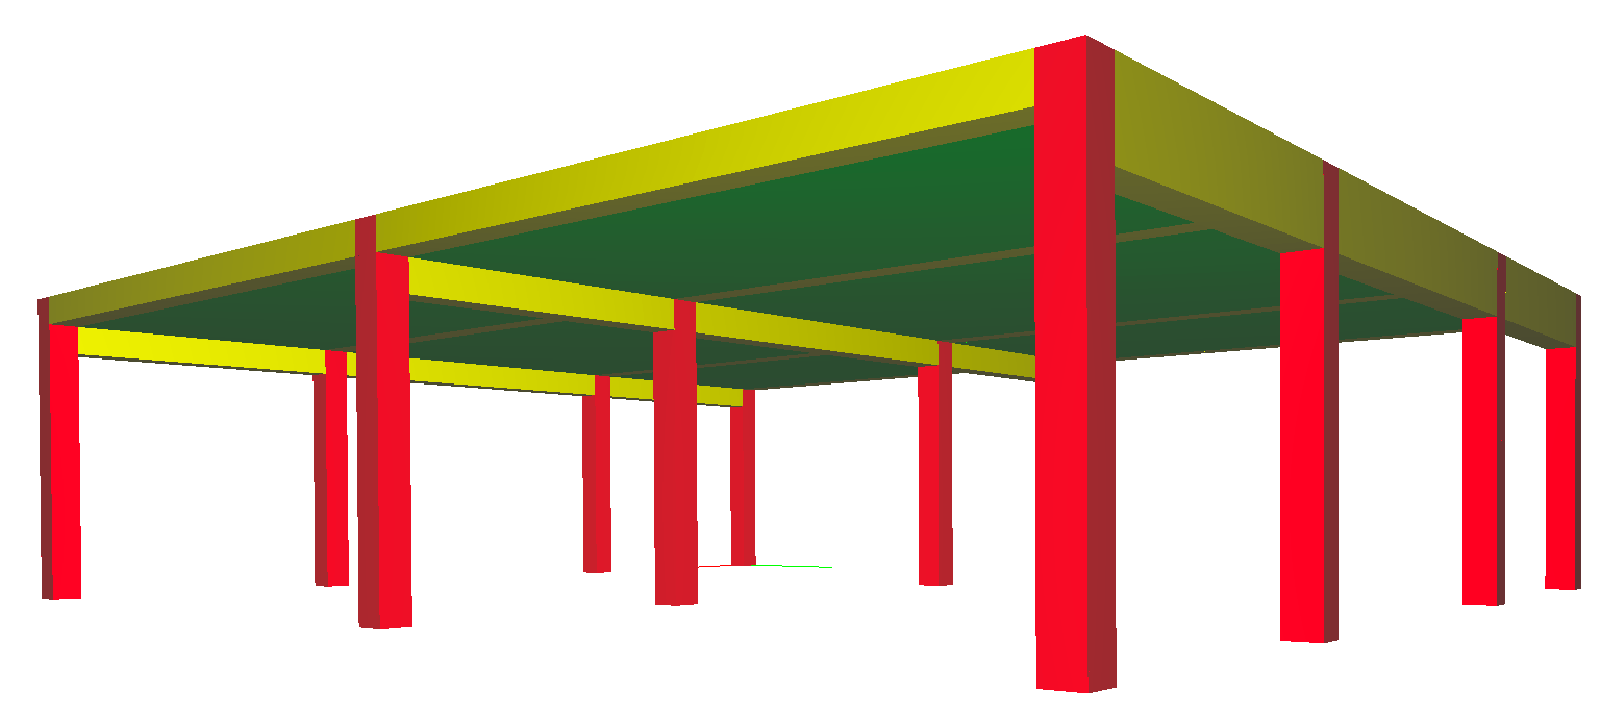
\includegraphics[width=\linewidth]{chapter-05/figs/frame1} 
   \caption{\sf frame = STRUCT(pillars, trusses, trusses1, floorslab);}.}
   \label{fig:example}
\end{figure}
\subsection*{Assembly combinator {\sf STRUCT}}\label{sect:5-1-1}

We have already come across the |STRUCT| function, one of more important |Plasm| operators. In particular, we already know that |STRUCT| is used to assembly geometric objects into a single object. In Julia |Plasm| both the input and the output objects are of recursive |Hpc| type.

In geometric modeling of complex assemblies the geometric and graphics
programmer makes wide use of the \emph{hierarchical scene
graphs}~\cite{Wernecke:94:TIM,Sowizral:2000:J3DAPI} or hierarchical
structures~\cite{Gaskins92}, where sub-assemblies are defined in \emph{local}
coordinates, and are transformed into the coordinate frame of the
output assembly by explicitly using proper coordinate
transformations.  

It is worth noting that such “modeling transformations" --- as they are called in graphical systems --- are left entirely to programmer's responsibility.  


\begin{figure}[htbp] %  figure placement: here, top, bottom, or page
   \sidecaption[t]
   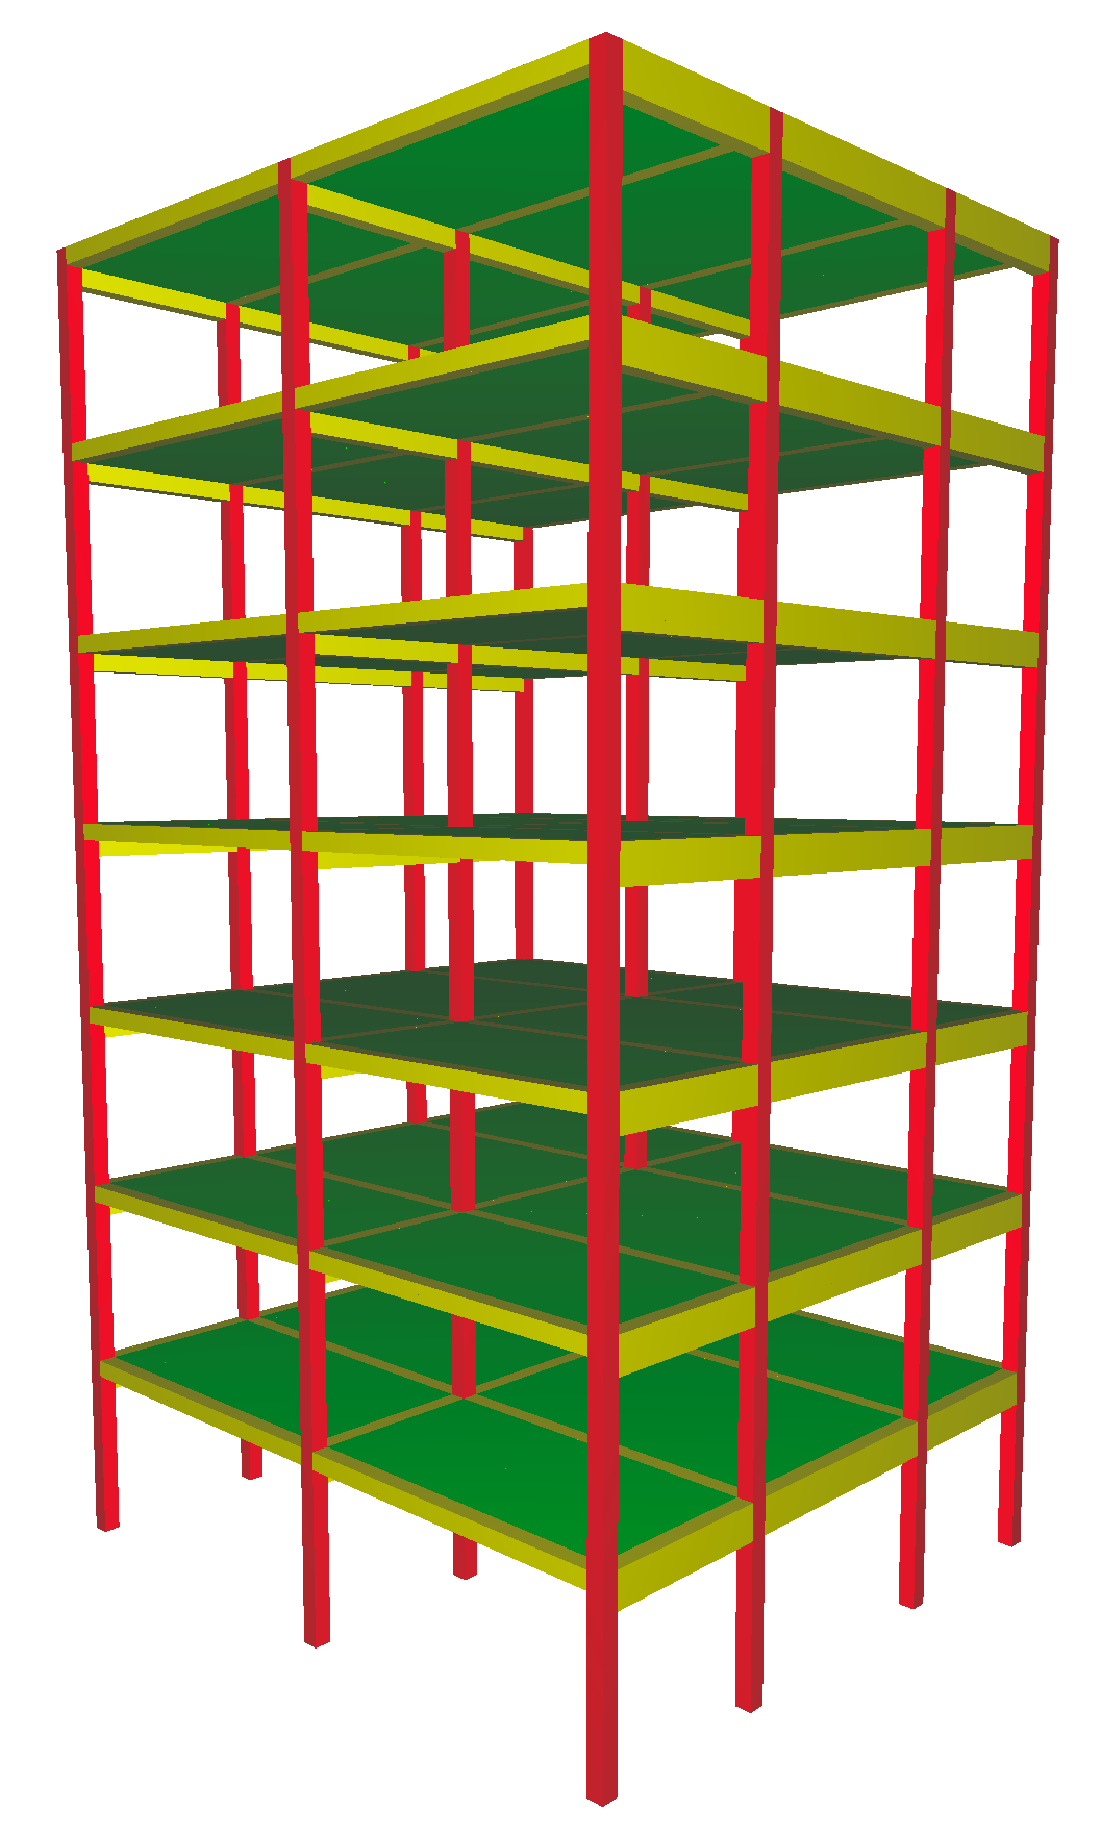
\includegraphics[width=0.6\linewidth]{chapter-05/figs/skeleton1} 
   \caption{\sf skeleton = STRUCT(NN(7)([frame, T(3)(3.3)])));}.}
   \label{fig:5:1:skeleton}
\end{figure}

\begin{coding}[Building skeleton]\label{5:1:skeleton}
We assemble here a building skeleton model, by creating a |STRUCT| assembly generated by |n=7| instances of the Julia |Vector| made by the |Hpc| value |frame| and by the |MatrixNd| value |T(3)(3.3)| producing a translation in $z$ direction.
\begin{lstlisting}[language=JuliaLocal, style=julia, mathescape=true]
skeleton = STRUCT(NN(7)([frame, T(3)(3.3)]));
VIEW(skeleton, Dict("background_color"=>WHITE)
\end{lstlisting}
\end{coding}

Here the |STRUCT| semantics is very clear: the evaluated subexpression |NN(7)([frame, T(3)(3.3)])| is an array of type |Vector{Union{Hpc, MatrixNd}}| and contain 14 item with alternating types.  When |STRUCT| is evaluted on this vector, an |Hpc| node is generated, whose |MatrixNd| field contains a $4\times 4$ identity matrix, and the |childs| vector contains the reference to the first item of 


\subsection*{Alignment aggregators {\sf TOP, BOTTOM, LEFT, RIGTH}}\label{sect:5-1-1}


In the present section we discuss some simplified assembly operators, where the
coordinate transformations are computed automatically by the language.

|Plasm| has some predefined binary functions used to locate two complexes with respect each other.  In particular,
the second argument of such functions will be positioned either
|TOP| the first one, or |ABOVE|, or |LEFT|, or
|RIGHT|, or |UP|, or |DOWN|, respectively,
according to the alignment semantics given below.

Such relative positioning allows
for an easy construction of complex assemblies, without taking into account the local coordinate frames where the
sub-assemblies are defined.  In this way we avoid applying affine transformations as it is
conversely needed in hierarchical scene graphs.

\begin{coding}[alternate method for vertical aggregation]\
\begin{lstlisting}[language=JuliaLocal, style=julia, mathescape=true]
multifloor(model,n) = STRUCT(INSR(TOP)(N(n+1)(model))) #=
multifloor (generic function with 1 method)		  	   =#
VIEW(multifloor(frame,7))
\end{lstlisting}
The object generated here is equal to the |skeleton| model of Figure \ref{fig:5:1:skeleton}. 
\end{coding}

|TOP| is a binary function of two |Hpc| models that creates their vertical aggregation.
Any binary function is transformed in $n$-ary by the second order operator |INSR| (for \emph{insert right}). |INSR| is applied first to the operator argument to make $n$-ary, then to the list of objects the operator apply to.

|N(n)(value::Any)| is a |Plasm| function called $\#$ in classic |PLaSM|, that returns a list of |n| instances of |value|. 

\begin{definition}[Primitive {\sf ALIGN} function.]
Every pair of polyhedral complexes may be aligned along any given subset of coordinates by using the primitive binary function |ALIGN|. Such a second-order operator must be applied to a sequence of triples which define a specialized behavior for each affected coordinate.
\end{definition}

Each alignment directive along a coordinate must belong to the set
\[
[1,n] \times \{ |MIN,MED,MAX,K($\alpha$)|\} 
\times \{ |MIN,MED,MAX,K($\alpha$})|\}
\]
where |$\alpha$::Number|. The resulting specialized operator is then applied to a pair of |Hpc| values, and returns a single |Hpc|. 
\begin{lstlisting}[language=JuliaLocal, style=julia, mathescape=true]
TOP = ALIGN([[3, MAX, MIN], [1, MED, MED], [2, MED, MED]])
BOTTOM = ALIGN([[3, MIN, MAX], [1, MED, MED], [2, MED, MED]])
LEFT = ALIGN([[1, MIN, MAX], [3, MIN, MIN]])
RIGHT = ALIGN([[1, MAX, MIN], [3, MIN, MIN]])
UP = ALIGN([[2, MAX, MIN], [3, MIN, MIN]])
DOWN = ALIGN([[2, MIN, MAX], [3, MIN, MIN]])
# 294 (generic function with 1 method)
\end{lstlisting}


\begin{figure}[htbp] %  figure placement: here, top, bottom, or page
   \sidecaption[t]
   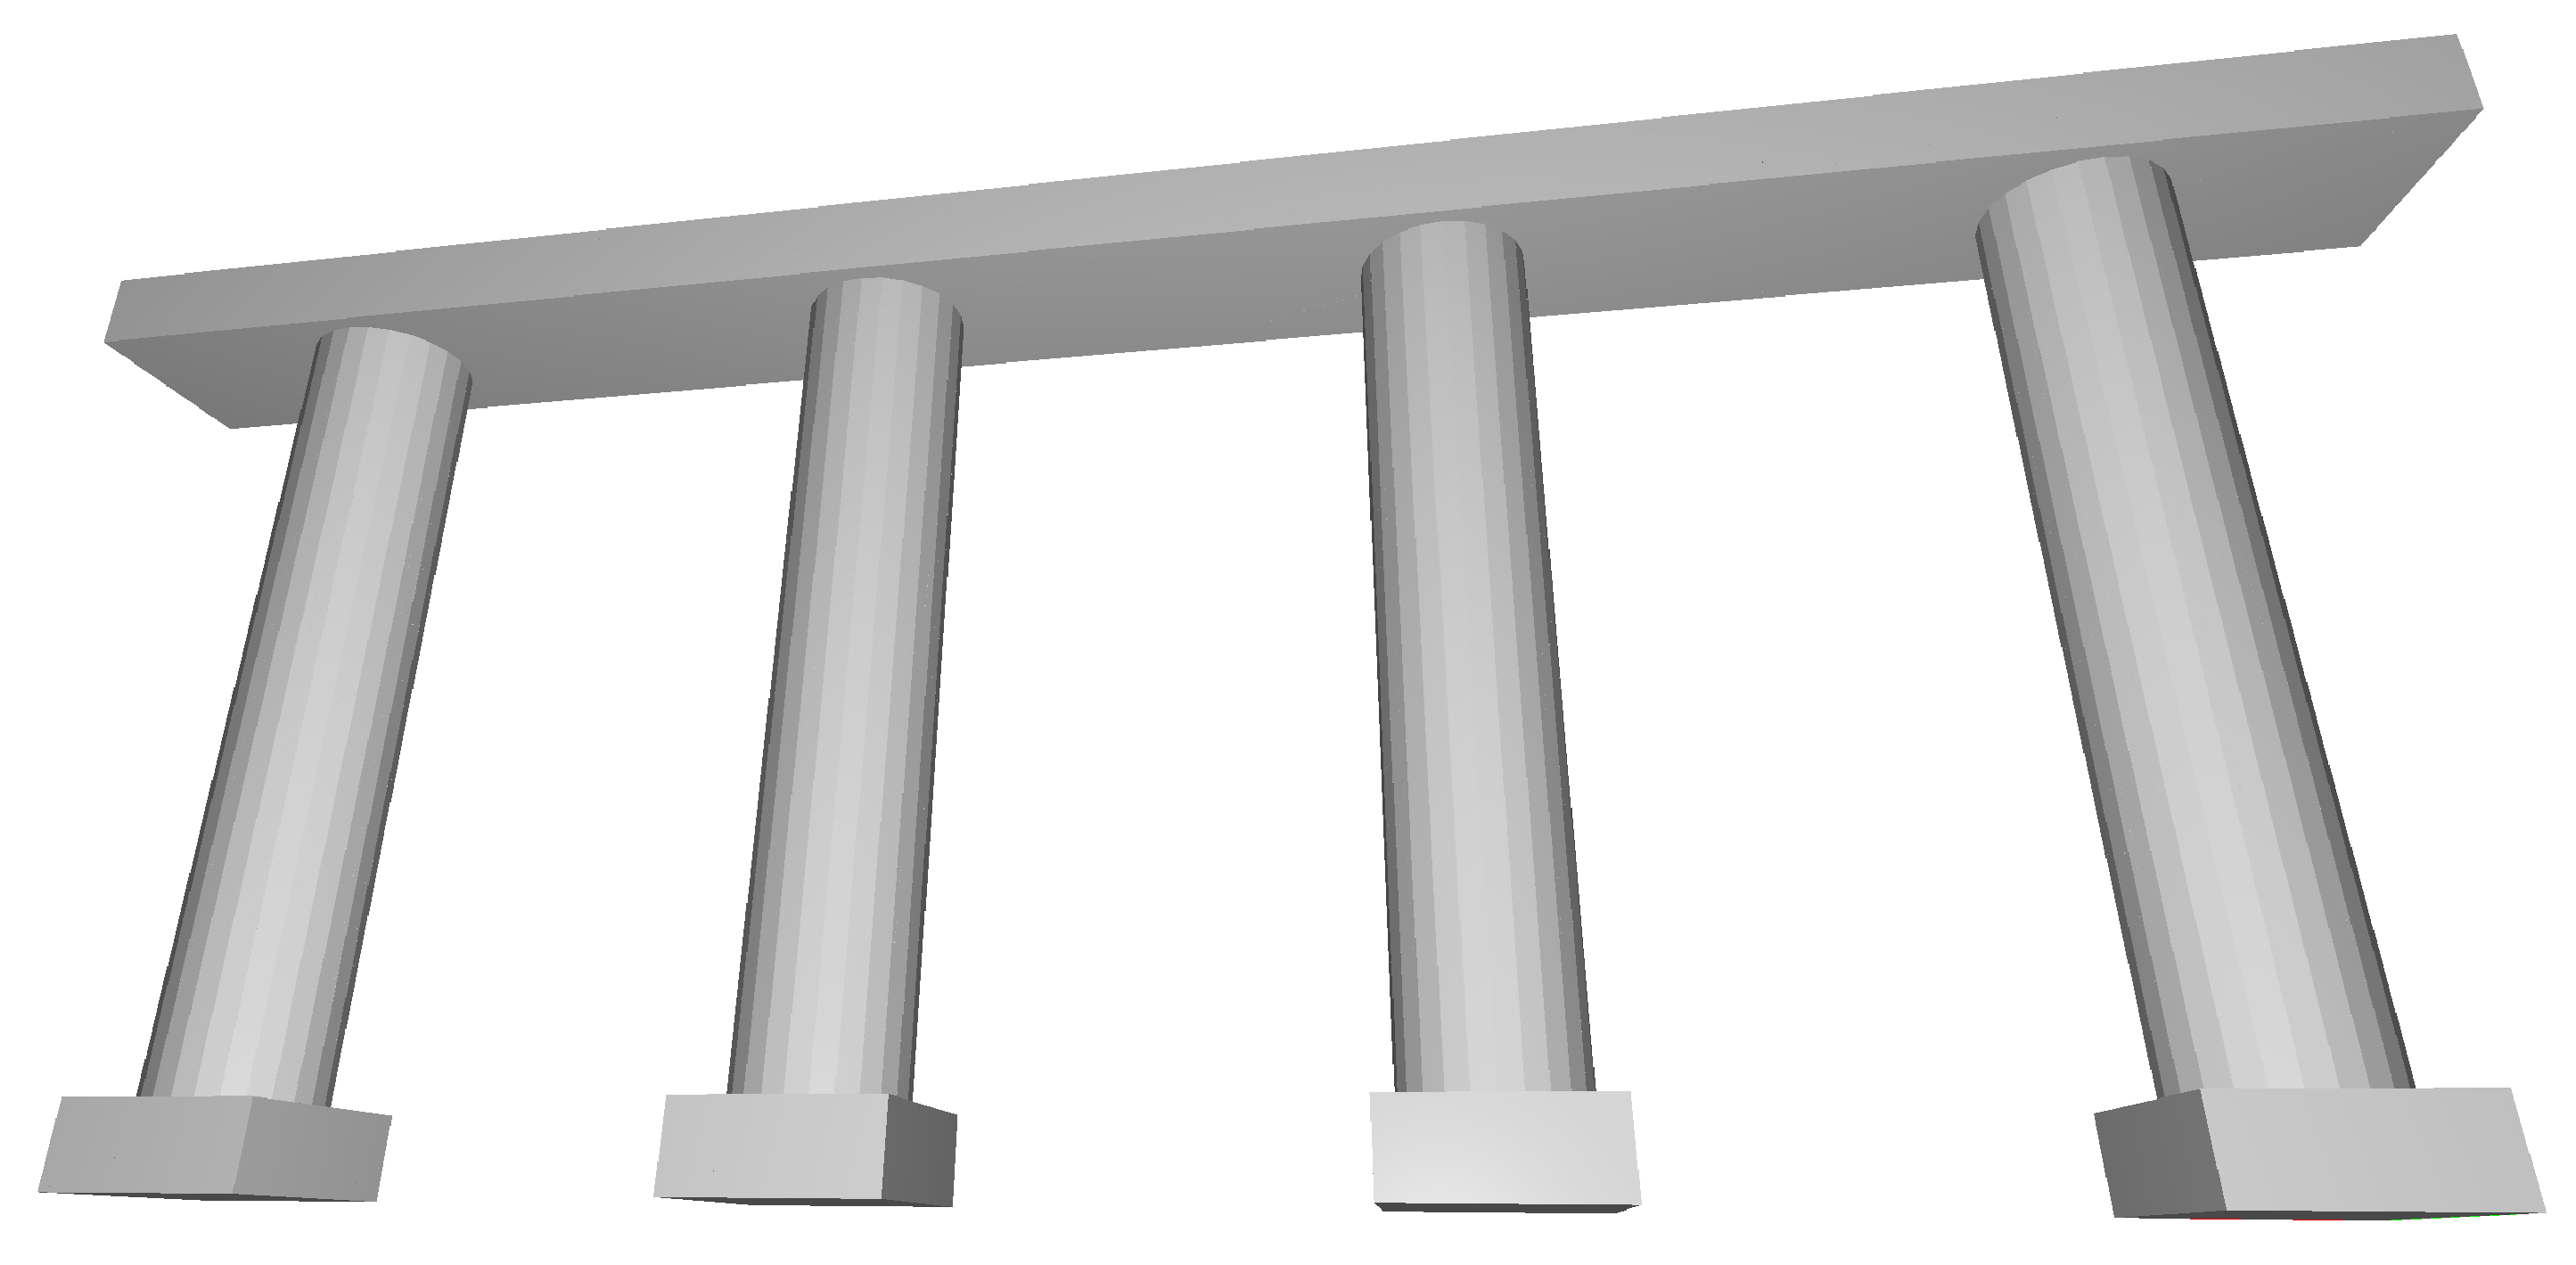
\includegraphics[width=\linewidth]{chapter-05/figs/fourcolumns} 
   \caption{\sf skeleton = STRUCT(NN(7)([frame, T(3)(3.3)])));}.}
   \label{fig:5:1:skeleton}
\end{figure}

\begin{coding}\
\begin{lstlisting}[language=JuliaLocal, style=julia, mathescape=true]
function Column(r::Float64,h::Float64)
	basis = CUBOID([ 2r*1.2, 2r*1.2, h/12 ]) 
	trunk = CYLINDER([ r, h/1.2 ])(24)
	capital = deepcopy(basis)
	beam = S(1)(3)(capital) 
	return INSR(TOP)([basis,trunk,capital,beam])
end
\end{lstlisting}

\begin{lstlisting}[language=JuliaLocal, style=julia, mathescape=true]
function ColRow(N::Int64)
	col = Column(1.0, 12.0)
	objs = [col for k in 1:N+1]
	return INSR(RIGHT)(objs)
end

VIEW(ColRow(4), Dict("background_color"=>WHITE)
\end{lstlisting}
\end{coding}


\section{ Plasm topological operators}\label{sect:5-2}


\section{ Linear and affine operators}\label{sect:5-3}


\section{ Manifold mapping}\label{sect:5-4}


\section{ Curve, surface, and solid methods}\label{sect:5-5}



% !TEX TS-program = xelatex

\chapter{Product assembly structure}
\label{chapt:6}

Models of assemblies are generated by aggregating subassemblies, each defined in its local coordinate system and relocated by affine transformations. This operation may be repeated hierarchically, with some subassemblies defined by aggregating simpler parts, and so on, until we get a set of elementary components that cannot be further disaggregated.
Two main advantages can be found in hierarchical modeling. Each elementary part and each assembly, at every hierarchical level, are defined independently from each other, using local coordinate frames suitably chosen to make their definition easier. Furthermore, only one copy of each component is used, and can be instanced in different locations and orientations, depending on how many times it is needed. In this chapter, after an overview of solid modeling data structures, the models of |Plasm|’s design datasets are discussed. 


\section{Hierarchical ssembly definition}\label{sect:6-1}


\section{Data structures in solid modeling}\label{sect:6-2}


\section{Structure in PHIGS and Plasm}\label{sect:6-3}


\section{Julia Plasm data structures}\label{sect:6-4}


\subsection{Hierarchical Polyhedral Complex (HPC)}\label{sect:6-4-1}


\subsection{Linear Algebraic Representation (LAR)}\label{sect:6-4-2}


\subsection{Geometric DataSet (GEO)}\label{sect:7-4-3}



% !TEX TS-program = xelatex

\chapter{Space arrangements}
\label{chapt:7}

The chapter introduces computational topology algorithms to discover the two-dimensional (2D)/3D space partition induced by a collection of geometric objects of dimension (1D)/2D, respectively. 
The data structures needed for such computational program are sparse arrays and their standard algebraic operations. In this chapter, we also introduce a novel approach to solid modeling based on piecewise-linear algebraic topology, that allows to treat rather general cellular complexes, with cells homeomorphic to polyhedra, i.e., to triangulable spaces, and hence possibly non-convex and multiply connected. The notions we deal with include geometric complexes, linear spaces of chains and cochains, the chain complex of linear operators between pairs of spaces, and their compositions. The discussion is restricted to piecewise-linear topology and to space dimensions less or equal to three. 

\section{ Space partition and enumeration}\label{sect:7-1}


\section{ Cellular and boundary models}\label{sect:7-2}


\section{ Arrangements and Lattices}\label{sect:7-3}


\section{ 2D and 3D Examples}\label{sect:7-4}



% !TEX TS-program = xelatex

\chapter{Boolean solid algebras}
\label{chapt:8}

Engineers conceived Solid Modeling as a rigorous and universal language for geometry-based engineering. Mathematically, all solid models are computer representations of elements of some algebraic systems that are constructed and maintained by algorithms corresponding to the operations in such algebra.
This chapter, in particular, focuses on the algebraic relationships between CSG (Constructive Solid Geometry) and boundary representations of piecewise-linear (PL) polyhedra. We show that the (regularized) arrangement of a given set of spatially instanced primitive shapes is isomorphic to the finite Boolean algebra of regularized sets containing all possible CSG representations with the same primitives.
In particular, we show that the boundary evaluation of any CSG representation with a finite number of primitives, once executed some point membership tests, reduces algebraically to the Julia form of Boolean operations on bit strings, sparse matrix-vector multiplication, and shape reconstruction from algebraic atoms. Along the way, we discuss eloquent examples.

 

\section{Constructive Solid Geometry (CSG)}\label{sect:8-1}


\section{Atoms and Generators }\label{sect:8-2}


\section{Finite Boolean Algebras}\label{sect:8-3}


\section{Computational Pipeline}\label{sect:8-4}



%%%%%%%%%%%%%%%%%%%%%part.tex%%%%%%%%%%%%%%%%%%%%%%%%%%%%%%%%%%
% 
% sample part title
%
% Use this file as a template for your own input.
%
%%%%%%%%%%%%%%%%%%%%%%%% Springer %%%%%%%%%%%%%%%%%%%%%%%%%%

\part{Polyhedral Modeling in AEC}

% !TEX TS-program = xelatex

\chapter{Building Information Modeling (BIM)}
\label{chapt:9}

The construction industry is nowadays undergoing its very own digital revolution, helped by its unique way of working with BIM systems whose elements are the digital prototypes of physical elements like columns, windows, walls, doors, and stairs. 
In this chapter, we outline the conceptual foundations and the down of the BIM attitude of the construction industry and discuss the birth of concepts like building objects. We also discuss the standardized taxonomy of building and space systems as set of subsystems devoted to the fulfillment of physical requirements with suitable performance levels. 
In particular, we show  by example how Julia |Plasm|, relying on its understand of topology and constructive techniques, may automatically transform the preliminary shape design of spaces into the generic geometry of building elements and subsystems (skeleton, envelope, internal partitions, horizontal floors, vertical communications).


\section{BIM history (Chuck Eastman, ...)}\label{sect:9-1}


\section{Building taxonomy (UNI 9838)}\label{sect:9-2}


\section{Building envelope}\label{sect:9-3}


\section{Building skeleton}\label{sect:9-4}


\section{Construction Process Modeling}\label{sect:9-5}



% !TEX TS-program = xelatex


\chapter{Industry Foundation Classes (IFC)}
\label{chapt:10}

The Industry Foundation Classes (IFC) are an open international standard for sharing Building Information Model (BIM) data.
IFC is a non-proprietary file format used to exchange building information models. IFC files can share data between different software applications, making it possible for multiple stakeholders to collaborate on BIM projects. Of course, we are mostly interested in the IFC transport of shape information.
In this chapter, we, therefore, investigate the Julia |Plasm| ability to implement in a few rows of parametric Julia code the classes and attributes of the |IfcShapeRepresentation|
entity for the various types of shape representation, including PointCloud, Curve, Surface, GeometricSet, GeometricCurveSet, Annotation2D, SurfaceModel, Tessellation, SolidModel, SweptSolid, AdvancedSweptSolid, Brep, CSG, Clipping, and BoundingBox. 

\section{Simple introduction to IFC}\label{sect:10-1}


\section{Data scheme for BIM collaboration}\label{sect:10-2}


\section{IfcShapeRepresentation (IFC 4.3.x: 8.18.3.14)}\label{sect:10-3}

\subsection{Representation identifiers}\label{sect:10-3-1}


\subsection{Representation types}\label{sect:10-3-2}


\subsection{Representation Examples}\label{sect:10-3-3}




\section{Plasm parametric programming to IFC}\label{sect:10-4}



%%%%%%%%%%%%%%%%%%%%%part.tex%%%%%%%%%%%%%%%%%%%%%%%%%%%%%%%%%%
% 
% sample part title
%
% Use this file as a template for your own input.
%
%%%%%%%%%%%%%%%%%%%%%%%% Springer %%%%%%%%%%%%%%%%%%%%%%%%%%

\part{Geometry from Point Cloud}


\chapter{Modeling from Point Clouds}\label{chapt:11}

At vero eos et accusamus et iusto odio dignissimos ducimus qui blanditiis praesentium voluptatum deleniti atque corrupti quos dolores et quas molestias excepturi sint occaecati cupiditate non provident, similique sunt in culpa qui officia deserunt mollitia animi, id est laborum et dolorum fuga. Et harum quidem rerum facilis est et expedita distinctio. Nam libero tempore, cum soluta nobis est eligendi optio cumque nihil impedit quo minus id quod maxime placeat facere possimus, omnis voluptas assumenda est, omnis dolor repellendus. Temporibus autem quibusdam et aut officiis debitis aut rerum necessitatibus saepe eveniet ut et voluptates repudiandae sint et molestiae non recusandae. 

\section{ Geometric survey}\label{sect:11-1}


\section{ Out-of-Core Potree dataset}\label{sect:11-2}


\section{ Multidimensional array store}\label{sect:11-3}


\section{ Mapping to solid models}\label{sect:11-4}

\bibliographystyle{spmpsci}
%\bibliographystyle{apacite}
\bibliography{plasmbook.bib}

%%%%%%%%%%%%%%%%%%%%% appendix.tex %%%%%%%%%%%%%%%%%%%%%%%%%%%%%%%%%
%
% sample appendix
%
% Use this file as a template for your own input.
%
%%%%%%%%%%%%%%%%%%%%%%%% Springer-Verlag %%%%%%%%%%%%%%%%%%%%%%%%%%

\appendix
\motto{All's well that ends well}
\chapter{Coding examples}


\backmatter%%%%%%%%%%%%%%%%%%%%%%%%%%%%%%%%%%%%%%%%%%%%%%%%%%%%%%%
%%%%%%%%%%%%%%%%%%%%%%acronym.tex%%%%%%%%%%%%%%%%%%%%%%%%%%%%%%%%%%%%%%%%%
% sample list of acronyms
%
% Use this file as a template for your own input.
%
%%%%%%%%%%%%%%%%%%%%%%%% Springer %%%%%%%%%%%%%%%%%%%%%%%%%%

\Extrachap{Glossary}


Use the template \emph{glossary.tex} together with the Springer document class SVMono (monograph-type books) or SVMult (edited books) to style your glossary in the Springer layout.


\runinhead{glossary term} Write here the description of the glossary term. Write here the description of the glossary term. Write here the description of the glossary term.

\runinhead{glossary term} Write here the description of the glossary term. Write here the description of the glossary term. Write here the description of the glossary term.

\runinhead{glossary term} Write here the description of the glossary term. Write here the description of the glossary term. Write here the description of the glossary term.

\runinhead{glossary term} Write here the description of the glossary term. Write here the description of the glossary term. Write here the description of the glossary term.

\runinhead{glossary term} Write here the description of the glossary term. Write here the description of the glossary term. Write here the description of the glossary term.
\include{solutions}
\printindex

%%%%%%%%%%%%%%%%%%%%%%%%%%%%%%%%%%%%%%%%%%%%%%%%%%%%%%%%%%%%%%%%%%%%%%

\end{document}




